\documentclass[twoside]{book}

% Packages required by doxygen
\usepackage{fixltx2e}
\usepackage{calc}
\usepackage{doxygen}
\usepackage[export]{adjustbox} % also loads graphicx
\usepackage{graphicx}
\usepackage[utf8]{inputenc}
\usepackage{makeidx}
\usepackage{multicol}
\usepackage{multirow}
\PassOptionsToPackage{warn}{textcomp}
\usepackage{textcomp}
\usepackage[nointegrals]{wasysym}
\usepackage[table]{xcolor}

% Font selection
\usepackage[T1]{fontenc}
\usepackage[scaled=.90]{helvet}
\usepackage{courier}
\usepackage{amssymb}
\usepackage{sectsty}
\renewcommand{\familydefault}{\sfdefault}
\allsectionsfont{%
  \fontseries{bc}\selectfont%
  \color{darkgray}%
}
\renewcommand{\DoxyLabelFont}{%
  \fontseries{bc}\selectfont%
  \color{darkgray}%
}
\newcommand{\+}{\discretionary{\mbox{\scriptsize$\hookleftarrow$}}{}{}}

% Page & text layout
\usepackage{geometry}
\geometry{%
  a4paper,%
  top=2.5cm,%
  bottom=2.5cm,%
  left=2.5cm,%
  right=2.5cm%
}
\tolerance=750
\hfuzz=15pt
\hbadness=750
\setlength{\emergencystretch}{15pt}
\setlength{\parindent}{0cm}
\setlength{\parskip}{3ex plus 2ex minus 2ex}
\makeatletter
\renewcommand{\paragraph}{%
  \@startsection{paragraph}{4}{0ex}{-1.0ex}{1.0ex}{%
    \normalfont\normalsize\bfseries\SS@parafont%
  }%
}
\renewcommand{\subparagraph}{%
  \@startsection{subparagraph}{5}{0ex}{-1.0ex}{1.0ex}{%
    \normalfont\normalsize\bfseries\SS@subparafont%
  }%
}
\makeatother

% Headers & footers
\usepackage{fancyhdr}
\pagestyle{fancyplain}
\fancyhead[LE]{\fancyplain{}{\bfseries\thepage}}
\fancyhead[CE]{\fancyplain{}{}}
\fancyhead[RE]{\fancyplain{}{\bfseries\leftmark}}
\fancyhead[LO]{\fancyplain{}{\bfseries\rightmark}}
\fancyhead[CO]{\fancyplain{}{}}
\fancyhead[RO]{\fancyplain{}{\bfseries\thepage}}
\fancyfoot[LE]{\fancyplain{}{}}
\fancyfoot[CE]{\fancyplain{}{}}
\fancyfoot[RE]{\fancyplain{}{\bfseries\scriptsize Generated by Doxygen }}
\fancyfoot[LO]{\fancyplain{}{\bfseries\scriptsize Generated by Doxygen }}
\fancyfoot[CO]{\fancyplain{}{}}
\fancyfoot[RO]{\fancyplain{}{}}
\renewcommand{\footrulewidth}{0.4pt}
\renewcommand{\chaptermark}[1]{%
  \markboth{#1}{}%
}
\renewcommand{\sectionmark}[1]{%
  \markright{\thesection\ #1}%
}

% Indices & bibliography
\usepackage{natbib}
\usepackage[titles]{tocloft}
\setcounter{tocdepth}{3}
\setcounter{secnumdepth}{5}
\makeindex

% Custom commands
\newcommand{\clearemptydoublepage}{%
  \newpage{\pagestyle{empty}\cleardoublepage}%
}

\usepackage{caption}
\captionsetup{labelsep=space,justification=centering,font={bf},singlelinecheck=off,skip=4pt,position=top}

%===== C O N T E N T S =====

\begin{document}

% Titlepage & ToC
\pagenumbering{alph}
\begin{titlepage}
\vspace*{7cm}
\begin{center}%
{\Large Chord V \\[1ex]\large 0.\+1 }\\
\vspace*{1cm}
{\large Generated by Doxygen 1.8.13}\\
\end{center}
\end{titlepage}
\clearemptydoublepage
\pagenumbering{roman}
\tableofcontents
\clearemptydoublepage
\pagenumbering{arabic}

%--- Begin generated contents ---
\chapter{General documentation for ChordV developpers}
\label{index}\section{Introduction}\label{index_Introduction}
ChordV allow to edit song booklet with lyrics and text of song, or only chords output, or only Luyrics output All feature are accessible from the \doxyref{Main\+Window}{p.}{class_main_window}. All the \doxyref{Main\+Window}{p.}{class_main_window} features are accessible from Menu There are many mode \+:
\begin{DoxyItemize}
\item Edition mode where users can enter text, chords and lyrics
\item Lyrics mode where users can define the Lyrics mode booklets
\item Text mode where users can define the Text booklets
\item Text and Chors mode where users can define the options for the Text and chord booklets In preferences dialog option you can design the general booklet definition and change the behaviour for each booklet from the behaviour defined in option.
\end{DoxyItemize}\subsection{Convention}\label{index_Convention}

\begin{DoxyItemize}
\item {\bfseries language} \+: is always the name of the language in the language. For example Français or English
\item {\bfseries codelang} \+: is always te code lang for a language. For example fr or en
\end{DoxyItemize}\section{Edition Mode}\label{index_Edition}
\section{Configuration Mode}\label{index_Configuration}

\chapter{Namespace Index}
\section{Namespace List}
Here is a list of all namespaces with brief descriptions\+:\begin{DoxyCompactList}
\item\contentsline{section}{\textbf{ Ui} }{\pageref{namespace_ui}}{}
\end{DoxyCompactList}

\chapter{Hierarchical Index}
\section{Class Hierarchy}
This inheritance list is sorted roughly, but not completely, alphabetically\+:\begin{DoxyCompactList}
\item \contentsline{section}{Chord\+Detector}{\pageref{class_chord_detector}}{}
\item \contentsline{section}{Chord\+Util}{\pageref{class_chord_util}}{}
\item \contentsline{section}{Const}{\pageref{class_const}}{}
\item \contentsline{section}{Lang\+Notes}{\pageref{class_lang_notes}}{}
\item \contentsline{section}{Language}{\pageref{class_language}}{}
\item \contentsline{section}{Normalize\+List}{\pageref{class_normalize_list}}{}
\item \contentsline{section}{Pdf\+Viewer}{\pageref{class_pdf_viewer}}{}
\item Q\+Combo\+Box\begin{DoxyCompactList}
\item \contentsline{section}{Page\+Size}{\pageref{class_page_size}}{}
\item \contentsline{section}{Vertical\+Spacing}{\pageref{class_vertical_spacing}}{}
\end{DoxyCompactList}
\item Q\+Dialog\begin{DoxyCompactList}
\item \contentsline{section}{Dialog\+About}{\pageref{class_dialog_about}}{}
\item \contentsline{section}{Dialog\+Bar}{\pageref{class_dialog_bar}}{}
\item \contentsline{section}{Dialog\+Change\+Chord\+Name}{\pageref{class_dialog_change_chord_name}}{}
\item \contentsline{section}{Dialog\+Choose\+Good\+Chord}{\pageref{class_dialog_choose_good_chord}}{}
\item \contentsline{section}{Dialog\+Chord\+Definition}{\pageref{class_dialog_chord_definition}}{}
\item \contentsline{section}{Dialog\+Configuration}{\pageref{class_dialog_configuration}}{}
\item \contentsline{section}{Dialog\+Documentation}{\pageref{class_dialog_documentation}}{}
\item \contentsline{section}{Dialog\+New\+Song}{\pageref{class_dialog_new_song}}{}
\item \contentsline{section}{Dialog\+Replace}{\pageref{class_dialog_replace}}{}
\item \contentsline{section}{Dialog\+Search}{\pageref{class_dialog_search}}{}
\item \contentsline{section}{Dialog\+System\+Info}{\pageref{class_dialog_system_info}}{}
\item \contentsline{section}{Dialog\+Transpose}{\pageref{class_dialog_transpose}}{}
\item \contentsline{section}{Dialog\+Two\+Lines\+To\+Chord\+Pro}{\pageref{class_dialog_two_lines_to_chord_pro}}{}
\item \contentsline{section}{Font\+Chooser}{\pageref{class_font_chooser}}{}
\end{DoxyCompactList}
\item Q\+Font\+Dialog\begin{DoxyCompactList}
\item \contentsline{section}{Font\+Dialog}{\pageref{class_font_dialog}}{}
\end{DoxyCompactList}
\item Q\+Graphics\+View\begin{DoxyCompactList}
\item \contentsline{section}{Neck}{\pageref{class_neck}}{}
\end{DoxyCompactList}
\item Q\+Label\begin{DoxyCompactList}
\item \contentsline{section}{Example\+Label}{\pageref{class_example_label}}{}
\end{DoxyCompactList}
\item Q\+Line\+Edit\begin{DoxyCompactList}
\item \contentsline{section}{Line\+Edit\+Test}{\pageref{class_line_edit_test}}{}
\end{DoxyCompactList}
\item Q\+Main\+Window\begin{DoxyCompactList}
\item \contentsline{section}{Main\+Window}{\pageref{class_main_window}}{}
\end{DoxyCompactList}
\item Q\+Object\begin{DoxyCompactList}
\item \contentsline{section}{Processor}{\pageref{class_processor}}{}
\begin{DoxyCompactList}
\item \contentsline{section}{Processor\+Chord}{\pageref{class_processor_chord}}{}
\item \contentsline{section}{Processor\+Lyrics}{\pageref{class_processor_lyrics}}{}
\item \contentsline{section}{Processor\+Text}{\pageref{class_processor_text}}{}
\end{DoxyCompactList}
\end{DoxyCompactList}
\item Q\+Settings\begin{DoxyCompactList}
\item \contentsline{section}{Settings}{\pageref{class_settings}}{}
\end{DoxyCompactList}
\item Q\+String\begin{DoxyCompactList}
\item \contentsline{section}{Chord}{\pageref{class_chord}}{}
\end{DoxyCompactList}
\item Q\+Syntax\+Highlighter\begin{DoxyCompactList}
\item \contentsline{section}{Editor\+Highlighter}{\pageref{class_editor_highlighter}}{}
\end{DoxyCompactList}
\item Q\+Text\+Edit\begin{DoxyCompactList}
\item \contentsline{section}{Log\+Messages}{\pageref{class_log_messages}}{}
\item \contentsline{section}{Text\+Edit}{\pageref{class_text_edit}}{}
\end{DoxyCompactList}
\item Q\+Tool\+Button\begin{DoxyCompactList}
\item \contentsline{section}{Color\+Button}{\pageref{class_color_button}}{}
\item \contentsline{section}{Font\+Button}{\pageref{class_font_button}}{}
\item \contentsline{section}{Image\+Button}{\pageref{class_image_button}}{}
\end{DoxyCompactList}
\item Q\+Widget\begin{DoxyCompactList}
\item \contentsline{section}{Chord\+Diagram}{\pageref{class_chord_diagram}}{}
\item \contentsline{section}{Form\+Config}{\pageref{class_form_config}}{}
\begin{DoxyCompactList}
\item \contentsline{section}{Chord\+Config}{\pageref{class_chord_config}}{}
\item \contentsline{section}{Lyrics\+Config}{\pageref{class_lyrics_config}}{}
\item \contentsline{section}{Memory\+Config}{\pageref{class_memory_config}}{}
\item \contentsline{section}{Text\+Config}{\pageref{class_text_config}}{}
\end{DoxyCompactList}
\item \contentsline{section}{Form\+Editor}{\pageref{class_form_editor}}{}
\item \contentsline{section}{Form\+Input\+Output\+Chord}{\pageref{class_form_input_output_chord}}{}
\item \contentsline{section}{Spin\+Box\+Unit}{\pageref{class_spin_box_unit}}{}
\end{DoxyCompactList}
\end{DoxyCompactList}

\chapter{Class Index}
\section{Class List}
Here are the classes, structs, unions and interfaces with brief descriptions\+:\begin{DoxyCompactList}
\item\contentsline{section}{\textbf{ Chord} \\*The \doxyref{Chord}{p.}{class_chord} class Manipulate the chords in D,D6,D7m,D7-\/,D7(\+V) on the Vth fret, D7x2 \+: on two bear, D7\+:2 on 1/2 bar }{\pageref{class_chord}}{}
\item\contentsline{section}{\textbf{ Chord\+Config} }{\pageref{class_chord_config}}{}
\item\contentsline{section}{\textbf{ Chord\+Detector} \\*Allow to detect a chord from list\+Notes. It is used on guitar neck to transform a list of notes to Q\+String\+List of chords given by the method \doxyref{detect\+Chord()}{p.}{class_chord_detector_a1d17c7c43eadf715a10a2910a5593fae}; The list of notes given to constructor are for example A, E, F The algorythm is given buy the tblscitype of the ChordV database. The ChordV Database containes two tables \+: tblscitype and Chords }{\pageref{class_chord_detector}}{}
\item\contentsline{section}{\textbf{ Chord\+Diagram} \\*Widget class usable in designer to show chords in Qtt Designer }{\pageref{class_chord_diagram}}{}
\item\contentsline{section}{\textbf{ Chord\+Util} \\*Some utilities }{\pageref{class_chord_util}}{}
\item\contentsline{section}{\textbf{ Color\+Button} \\*Allows to draw the color of Q\+Tool\+Button when user choose a color after click on button. The allow to show the color chooser by the button. This class is Qt\+Designer/\+Qt\+Creator complient }{\pageref{class_color_button}}{}
\item\contentsline{section}{\textbf{ Const} \\*Set of constant classes }{\pageref{class_const}}{}
\item\contentsline{section}{\textbf{ Dialog\+About} \\*Show the Dialog about }{\pageref{class_dialog_about}}{}
\item\contentsline{section}{\textbf{ Dialog\+Bar} \\*Allow to choose the bar dialog for example 4/4 or 3/4 information }{\pageref{class_dialog_bar}}{}
\item\contentsline{section}{\textbf{ Dialog\+Change\+Chord\+Name} \\*Used to change language of name of a chord by transposition }{\pageref{class_dialog_change_chord_name}}{}
\item\contentsline{section}{\textbf{ Dialog\+Choose\+Good\+Chord} }{\pageref{class_dialog_choose_good_chord}}{}
\item\contentsline{section}{\textbf{ Dialog\+Chord\+Definition} }{\pageref{class_dialog_chord_definition}}{}
\item\contentsline{section}{\textbf{ Dialog\+Configuration} }{\pageref{class_dialog_configuration}}{}
\item\contentsline{section}{\textbf{ Dialog\+Documentation} }{\pageref{class_dialog_documentation}}{}
\item\contentsline{section}{\textbf{ Dialog\+New\+Song} \\*This Dialog ask title, sybtitel, compress output yes or no, and column number for a song it provide a S\+I\+G\+N\+AL whe you clik on Insert button }{\pageref{class_dialog_new_song}}{}
\item\contentsline{section}{\textbf{ Dialog\+Replace} \\*Allo to search and replace words in Editor }{\pageref{class_dialog_replace}}{}
\item\contentsline{section}{\textbf{ Dialog\+Search} \\*Allow to search word in Editor }{\pageref{class_dialog_search}}{}
\item\contentsline{section}{\textbf{ Dialog\+System\+Info} \\*This dialog show a set of system informations like date of compilation, release version, Git S\+H\+A1 version, program arguments, configuration file, Database location, P\+ID of process, location of language information }{\pageref{class_dialog_system_info}}{}
\item\contentsline{section}{\textbf{ Dialog\+Transpose} \\*Dialog class to ask how many chroma negative or positive the user wants to transpose. It ask if the chord has to be with parenthesis or no and ask if just the current chord has to print translated, all the chord in the current line, all the chord on the current song or all the chord of the current booklet }{\pageref{class_dialog_transpose}}{}
\item\contentsline{section}{\textbf{ Dialog\+Two\+Lines\+To\+Chord\+Pro} \\*Utility to convert song in two lines \+: }{\pageref{class_dialog_two_lines_to_chord_pro}}{}
\item\contentsline{section}{\textbf{ Editor\+Highlighter} }{\pageref{class_editor_highlighter}}{}
\item\contentsline{section}{\textbf{ Example\+Label} }{\pageref{class_example_label}}{}
\item\contentsline{section}{\textbf{ Font\+Button} }{\pageref{class_font_button}}{}
\item\contentsline{section}{\textbf{ Font\+Chooser} }{\pageref{class_font_chooser}}{}
\item\contentsline{section}{\textbf{ Font\+Dialog} \\*Derived class from Q\+Font\+Dialog to force Q\+Font\+Dialog to be a Q\+Widget that can be included as a promoted Widget }{\pageref{class_font_dialog}}{}
\item\contentsline{section}{\textbf{ Form\+Config} \\*Manage the display of configuration of attributes \+: (Color, Fonts, ...) for the definition of each booklet. It is used in Preference and also on each project }{\pageref{class_form_config}}{}
\item\contentsline{section}{\textbf{ Form\+Editor} \\*Manage }{\pageref{class_form_editor}}{}
\item\contentsline{section}{\textbf{ Form\+Input\+Output\+Chord} }{\pageref{class_form_input_output_chord}}{}
\item\contentsline{section}{\textbf{ Image\+Button} }{\pageref{class_image_button}}{}
\item\contentsline{section}{\textbf{ Lang\+Notes} }{\pageref{class_lang_notes}}{}
\item\contentsline{section}{\textbf{ Language} \\*Manage the translation files }{\pageref{class_language}}{}
\item\contentsline{section}{\textbf{ Line\+Edit\+Test} }{\pageref{class_line_edit_test}}{}
\item\contentsline{section}{\textbf{ Log\+Messages} }{\pageref{class_log_messages}}{}
\item\contentsline{section}{\textbf{ Lyrics\+Config} }{\pageref{class_lyrics_config}}{}
\item\contentsline{section}{\textbf{ Main\+Window} \\*The \doxyref{Main\+Window}{p.}{class_main_window} class }{\pageref{class_main_window}}{}
\item\contentsline{section}{\textbf{ Memory\+Config} }{\pageref{class_memory_config}}{}
\item\contentsline{section}{\textbf{ Neck} \\*Derivated of graphics\+View to allow to show a guitar neck and analyse the string touched to calculate chord }{\pageref{class_neck}}{}
\item\contentsline{section}{\textbf{ Normalize\+List} }{\pageref{class_normalize_list}}{}
\item\contentsline{section}{\textbf{ Page\+Size} \\*Q\+Combobox derived type containing list of format like A4 A4 B2 ... the method get the size }{\pageref{class_page_size}}{}
\item\contentsline{section}{\textbf{ Pdf\+Viewer} }{\pageref{class_pdf_viewer}}{}
\item\contentsline{section}{\textbf{ Processor} }{\pageref{class_processor}}{}
\item\contentsline{section}{\textbf{ Processor\+Chord} }{\pageref{class_processor_chord}}{}
\item\contentsline{section}{\textbf{ Processor\+Lyrics} }{\pageref{class_processor_lyrics}}{}
\item\contentsline{section}{\textbf{ Processor\+Text} }{\pageref{class_processor_text}}{}
\item\contentsline{section}{\textbf{ Settings} \\*Derivate the Q\+Settings class by forcing I\+NI format when constructor is called whith a file name }{\pageref{class_settings}}{}
\item\contentsline{section}{\textbf{ Spin\+Box\+Unit} }{\pageref{class_spin_box_unit}}{}
\item\contentsline{section}{\textbf{ Text\+Config} }{\pageref{class_text_config}}{}
\item\contentsline{section}{\textbf{ Text\+Edit} }{\pageref{class_text_edit}}{}
\item\contentsline{section}{\textbf{ Vertical\+Spacing} }{\pageref{class_vertical_spacing}}{}
\end{DoxyCompactList}

\chapter{File Index}
\section{File List}
Here is a list of all files with brief descriptions\+:\begin{DoxyCompactList}
\item\contentsline{section}{src/\textbf{ chord.\+cpp} }{\pageref{chord_8cpp}}{}
\item\contentsline{section}{src/\textbf{ chord.\+h} }{\pageref{chord_8h}}{}
\item\contentsline{section}{src/\textbf{ chordconfig.\+cpp} }{\pageref{chordconfig_8cpp}}{}
\item\contentsline{section}{src/\textbf{ chordconfig.\+h} }{\pageref{chordconfig_8h}}{}
\item\contentsline{section}{src/\textbf{ Chord\+Detector.\+cpp} }{\pageref{_chord_detector_8cpp}}{}
\item\contentsline{section}{src/\textbf{ Chord\+Detector.\+h} }{\pageref{_chord_detector_8h}}{}
\item\contentsline{section}{src/\textbf{ chorddiagram.\+cpp} }{\pageref{chorddiagram_8cpp}}{}
\item\contentsline{section}{src/\textbf{ chorddiagram.\+h} }{\pageref{chorddiagram_8h}}{}
\item\contentsline{section}{src/\textbf{ chordutil.\+cpp} }{\pageref{chordutil_8cpp}}{}
\item\contentsline{section}{src/\textbf{ chordutil.\+h} }{\pageref{chordutil_8h}}{}
\item\contentsline{section}{src/\textbf{ colorbutton.\+cpp} }{\pageref{colorbutton_8cpp}}{}
\item\contentsline{section}{src/\textbf{ colorbutton.\+h} }{\pageref{colorbutton_8h}}{}
\item\contentsline{section}{src/\textbf{ const.\+h} }{\pageref{const_8h}}{}
\item\contentsline{section}{src/\textbf{ dialogabout.\+cpp} }{\pageref{dialogabout_8cpp}}{}
\item\contentsline{section}{src/\textbf{ dialogabout.\+h} }{\pageref{dialogabout_8h}}{}
\item\contentsline{section}{src/\textbf{ dialogbar.\+cpp} }{\pageref{dialogbar_8cpp}}{}
\item\contentsline{section}{src/\textbf{ dialogbar.\+h} }{\pageref{dialogbar_8h}}{}
\item\contentsline{section}{src/\textbf{ dialogchangechordname.\+cpp} }{\pageref{dialogchangechordname_8cpp}}{}
\item\contentsline{section}{src/\textbf{ dialogchangechordname.\+h} }{\pageref{dialogchangechordname_8h}}{}
\item\contentsline{section}{src/\textbf{ dialogchoosegoodchord.\+cpp} }{\pageref{dialogchoosegoodchord_8cpp}}{}
\item\contentsline{section}{src/\textbf{ dialogchoosegoodchord.\+h} }{\pageref{dialogchoosegoodchord_8h}}{}
\item\contentsline{section}{src/\textbf{ dialogchorddefinition.\+cpp} }{\pageref{dialogchorddefinition_8cpp}}{}
\item\contentsline{section}{src/\textbf{ dialogchorddefinition.\+h} }{\pageref{dialogchorddefinition_8h}}{}
\item\contentsline{section}{src/\textbf{ dialogconfiguration.\+cpp} }{\pageref{dialogconfiguration_8cpp}}{}
\item\contentsline{section}{src/\textbf{ dialogconfiguration.\+h} }{\pageref{dialogconfiguration_8h}}{}
\item\contentsline{section}{src/\textbf{ dialogdocumentation.\+cpp} }{\pageref{dialogdocumentation_8cpp}}{}
\item\contentsline{section}{src/\textbf{ dialogdocumentation.\+h} }{\pageref{dialogdocumentation_8h}}{}
\item\contentsline{section}{src/\textbf{ dialognewsong.\+cpp} }{\pageref{dialognewsong_8cpp}}{}
\item\contentsline{section}{src/\textbf{ dialognewsong.\+h} }{\pageref{dialognewsong_8h}}{}
\item\contentsline{section}{src/\textbf{ dialogreplace.\+cpp} }{\pageref{dialogreplace_8cpp}}{}
\item\contentsline{section}{src/\textbf{ dialogreplace.\+h} }{\pageref{dialogreplace_8h}}{}
\item\contentsline{section}{src/\textbf{ dialogsearch.\+cpp} }{\pageref{dialogsearch_8cpp}}{}
\item\contentsline{section}{src/\textbf{ dialogsearch.\+h} }{\pageref{dialogsearch_8h}}{}
\item\contentsline{section}{src/\textbf{ dialogsysteminfo.\+cpp} }{\pageref{dialogsysteminfo_8cpp}}{}
\item\contentsline{section}{src/\textbf{ dialogsysteminfo.\+h} }{\pageref{dialogsysteminfo_8h}}{}
\item\contentsline{section}{src/\textbf{ dialogtranspose.\+cpp} }{\pageref{dialogtranspose_8cpp}}{}
\item\contentsline{section}{src/\textbf{ dialogtranspose.\+h} }{\pageref{dialogtranspose_8h}}{}
\item\contentsline{section}{src/\textbf{ dialogtwolinestochordpro.\+cpp} }{\pageref{dialogtwolinestochordpro_8cpp}}{}
\item\contentsline{section}{src/\textbf{ dialogtwolinestochordpro.\+h} }{\pageref{dialogtwolinestochordpro_8h}}{}
\item\contentsline{section}{src/\textbf{ editorhighlighter.\+cpp} }{\pageref{editorhighlighter_8cpp}}{}
\item\contentsline{section}{src/\textbf{ editorhighlighter.\+h} }{\pageref{editorhighlighter_8h}}{}
\item\contentsline{section}{src/\textbf{ examplelabel.\+cpp} }{\pageref{examplelabel_8cpp}}{}
\item\contentsline{section}{src/\textbf{ examplelabel.\+h} }{\pageref{examplelabel_8h}}{}
\item\contentsline{section}{src/\textbf{ fontbutton.\+cpp} }{\pageref{fontbutton_8cpp}}{}
\item\contentsline{section}{src/\textbf{ fontbutton.\+h} }{\pageref{fontbutton_8h}}{}
\item\contentsline{section}{src/\textbf{ fontchooser.\+cpp} }{\pageref{fontchooser_8cpp}}{}
\item\contentsline{section}{src/\textbf{ fontchooser.\+h} }{\pageref{fontchooser_8h}}{}
\item\contentsline{section}{src/\textbf{ fontdialog.\+cpp} }{\pageref{fontdialog_8cpp}}{}
\item\contentsline{section}{src/\textbf{ fontdialog.\+h} }{\pageref{fontdialog_8h}}{}
\item\contentsline{section}{src/\textbf{ formconfig.\+cpp} }{\pageref{formconfig_8cpp}}{}
\item\contentsline{section}{src/\textbf{ formconfig.\+h} }{\pageref{formconfig_8h}}{}
\item\contentsline{section}{src/\textbf{ formeditor.\+cpp} }{\pageref{formeditor_8cpp}}{}
\item\contentsline{section}{src/\textbf{ formeditor.\+h} }{\pageref{formeditor_8h}}{}
\item\contentsline{section}{src/\textbf{ forminputoutputchord.\+cpp} }{\pageref{forminputoutputchord_8cpp}}{}
\item\contentsline{section}{src/\textbf{ forminputoutputchord.\+h} }{\pageref{forminputoutputchord_8h}}{}
\item\contentsline{section}{src/\textbf{ imagebutton.\+cpp} }{\pageref{imagebutton_8cpp}}{}
\item\contentsline{section}{src/\textbf{ imagebutton.\+h} }{\pageref{imagebutton_8h}}{}
\item\contentsline{section}{src/\textbf{ langnotes.\+cpp} }{\pageref{langnotes_8cpp}}{}
\item\contentsline{section}{src/\textbf{ langnotes.\+h} }{\pageref{langnotes_8h}}{}
\item\contentsline{section}{src/\textbf{ language.\+cpp} }{\pageref{language_8cpp}}{}
\item\contentsline{section}{src/\textbf{ language.\+h} }{\pageref{language_8h}}{}
\item\contentsline{section}{src/\textbf{ lineedittest.\+cpp} }{\pageref{lineedittest_8cpp}}{}
\item\contentsline{section}{src/\textbf{ lineedittest.\+h} }{\pageref{lineedittest_8h}}{}
\item\contentsline{section}{src/\textbf{ logmessages.\+cpp} }{\pageref{logmessages_8cpp}}{}
\item\contentsline{section}{src/\textbf{ logmessages.\+h} }{\pageref{logmessages_8h}}{}
\item\contentsline{section}{src/\textbf{ lyricsconfig.\+cpp} }{\pageref{lyricsconfig_8cpp}}{}
\item\contentsline{section}{src/\textbf{ lyricsconfig.\+h} }{\pageref{lyricsconfig_8h}}{}
\item\contentsline{section}{src/\textbf{ main.\+cpp} }{\pageref{main_8cpp}}{}
\item\contentsline{section}{src/\textbf{ mainwindow.\+cpp} }{\pageref{mainwindow_8cpp}}{}
\item\contentsline{section}{src/\textbf{ mainwindow.\+h} }{\pageref{mainwindow_8h}}{}
\item\contentsline{section}{src/\textbf{ memoryconfig.\+cpp} }{\pageref{memoryconfig_8cpp}}{}
\item\contentsline{section}{src/\textbf{ memoryconfig.\+h} }{\pageref{memoryconfig_8h}}{}
\item\contentsline{section}{src/\textbf{ neck.\+cpp} }{\pageref{neck_8cpp}}{}
\item\contentsline{section}{src/\textbf{ neck.\+h} }{\pageref{neck_8h}}{}
\item\contentsline{section}{src/\textbf{ normalizelist.\+cpp} }{\pageref{normalizelist_8cpp}}{}
\item\contentsline{section}{src/\textbf{ normalizelist.\+h} }{\pageref{normalizelist_8h}}{}
\item\contentsline{section}{src/\textbf{ pagesize.\+cpp} }{\pageref{pagesize_8cpp}}{}
\item\contentsline{section}{src/\textbf{ pagesize.\+h} }{\pageref{pagesize_8h}}{}
\item\contentsline{section}{src/\textbf{ pdfviewer.\+cpp} }{\pageref{pdfviewer_8cpp}}{}
\item\contentsline{section}{src/\textbf{ pdfviewer.\+h} }{\pageref{pdfviewer_8h}}{}
\item\contentsline{section}{src/\textbf{ processor.\+cpp} }{\pageref{processor_8cpp}}{}
\item\contentsline{section}{src/\textbf{ processor.\+h} }{\pageref{processor_8h}}{}
\item\contentsline{section}{src/\textbf{ processorchord.\+cpp} }{\pageref{processorchord_8cpp}}{}
\item\contentsline{section}{src/\textbf{ processorchord.\+h} }{\pageref{processorchord_8h}}{}
\item\contentsline{section}{src/\textbf{ processorlyrics.\+cpp} }{\pageref{processorlyrics_8cpp}}{}
\item\contentsline{section}{src/\textbf{ processorlyrics.\+h} }{\pageref{processorlyrics_8h}}{}
\item\contentsline{section}{src/\textbf{ processortext.\+cpp} }{\pageref{processortext_8cpp}}{}
\item\contentsline{section}{src/\textbf{ processortext.\+h} }{\pageref{processortext_8h}}{}
\item\contentsline{section}{src/\textbf{ settings.\+cpp} }{\pageref{settings_8cpp}}{}
\item\contentsline{section}{src/\textbf{ settings.\+h} }{\pageref{settings_8h}}{}
\item\contentsline{section}{src/\textbf{ spinboxunit.\+cpp} }{\pageref{spinboxunit_8cpp}}{}
\item\contentsline{section}{src/\textbf{ spinboxunit.\+h} }{\pageref{spinboxunit_8h}}{}
\item\contentsline{section}{src/\textbf{ textconfig.\+cpp} }{\pageref{textconfig_8cpp}}{}
\item\contentsline{section}{src/\textbf{ textconfig.\+h} }{\pageref{textconfig_8h}}{}
\item\contentsline{section}{src/\textbf{ textedit.\+cpp} }{\pageref{textedit_8cpp}}{}
\item\contentsline{section}{src/\textbf{ textedit.\+h} }{\pageref{textedit_8h}}{}
\item\contentsline{section}{src/\textbf{ version.\+h} }{\pageref{version_8h}}{}
\item\contentsline{section}{src/\textbf{ verticalspacing.\+cpp} }{\pageref{verticalspacing_8cpp}}{}
\item\contentsline{section}{src/\textbf{ verticalspacing.\+h} }{\pageref{verticalspacing_8h}}{}
\end{DoxyCompactList}

\chapter{Namespace Documentation}
\section{Ui Namespace Reference}
\label{namespace_ui}\index{Ui@{Ui}}

\chapter{Class Documentation}
\section{Chord Class Reference}
\label{class_chord}\index{Chord@{Chord}}


The \doxyref{Chord}{p.}{class_chord} class Manipulate the chords in D,D6,D7m,D7-\/,D7(\+V) on the Vth fret, D7x2 \+: on two bear, D7\+:2 on 1/2 bar.  




{\ttfamily \#include $<$chord.\+h$>$}



Inheritance diagram for Chord\+:\nopagebreak
\begin{figure}[H]
\begin{center}
\leavevmode
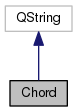
\includegraphics[width=130pt]{class_chord__inherit__graph}
\end{center}
\end{figure}


Collaboration diagram for Chord\+:\nopagebreak
\begin{figure}[H]
\begin{center}
\leavevmode
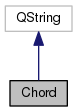
\includegraphics[width=130pt]{class_chord__coll__graph}
\end{center}
\end{figure}
\subsection*{Public Member Functions}
\begin{DoxyCompactItemize}
\item 
\textbf{ Chord} (Q\+String \textbf{ chord}, Q\+String codelang=\char`\"{}en\char`\"{})
\begin{DoxyCompactList}\small\item\em \doxyref{Chord}{p.}{class_chord} chord is defined by a chordname and the language name for the chord. \end{DoxyCompactList}\item 
Q\+String \textbf{ chord} ()
\begin{DoxyCompactList}\small\item\em chord \end{DoxyCompactList}\item 
Q\+String \textbf{ remove\+Rytm} ()
\begin{DoxyCompactList}\small\item\em remove\+Rytm \end{DoxyCompactList}\item 
int \textbf{ nb\+Bar} ()
\begin{DoxyCompactList}\small\item\em nb\+Bar \end{DoxyCompactList}\item 
int \textbf{ nb\+Beat} ()
\begin{DoxyCompactList}\small\item\em nb\+Beat \end{DoxyCompactList}\item 
Q\+String\+List \textbf{ to\+Strings} ()
\begin{DoxyCompactList}\small\item\em to\+Strings \end{DoxyCompactList}\item 
Q\+String \textbf{ fret} ()
\begin{DoxyCompactList}\small\item\em fret \end{DoxyCompactList}\item 
Q\+String \textbf{ To\+English} (Q\+String \textbf{ chord})
\begin{DoxyCompactList}\small\item\em To\+English. \end{DoxyCompactList}\item 
Q\+String \textbf{ name\+English} ()
\begin{DoxyCompactList}\small\item\em name\+English \end{DoxyCompactList}\item 
Q\+String \textbf{ name\+Locale} ()
\begin{DoxyCompactList}\small\item\em name\+Locale \end{DoxyCompactList}\item 
Q\+String \textbf{ pure\+Name\+Locale} ()
\begin{DoxyCompactList}\small\item\em pure\+Name\+Locale \end{DoxyCompactList}\item 
Q\+String \textbf{ pure\+Name\+English} ()
\begin{DoxyCompactList}\small\item\em pure\+Name\+English \end{DoxyCompactList}\item 
Q\+String \textbf{ up} ()
\begin{DoxyCompactList}\small\item\em up the name of the chord on the next fret \end{DoxyCompactList}\item 
Q\+String \textbf{ down} ()
\begin{DoxyCompactList}\small\item\em down the name of the chord on tne previous fret \end{DoxyCompactList}\item 
Q\+String \textbf{ transpose} (int degre, bool parentheses, Q\+String minfrom, Q\+String minto)
\begin{DoxyCompactList}\small\item\em transpose \+: transpose a chord \end{DoxyCompactList}\end{DoxyCompactItemize}
\subsection*{Static Public Member Functions}
\begin{DoxyCompactItemize}
\item 
static Q\+String\+List \textbf{ remove\+Dupplicate\+Whithout\+Rytm} (Q\+String\+List chords, Q\+String codelang)
\begin{DoxyCompactList}\small\item\em remove\+Dupplicate\+Whithout\+Rytm \end{DoxyCompactList}\item 
static Q\+String \textbf{ translate} (Q\+String \textbf{ chord}, Q\+String codelangfrom, Q\+String minfrom, Q\+String codelangto, Q\+String minto)
\begin{DoxyCompactList}\small\item\em translate \end{DoxyCompactList}\end{DoxyCompactItemize}


\subsection{Detailed Description}
The \doxyref{Chord}{p.}{class_chord} class Manipulate the chords in D,D6,D7m,D7-\/,D7(\+V) on the Vth fret, D7x2 \+: on two bear, D7\+:2 on 1/2 bar. 

\subsection{Constructor \& Destructor Documentation}
\mbox{\label{class_chord_ac61d5711e773d1d8203a6ee3d854142c}} 
\index{Chord@{Chord}!Chord@{Chord}}
\index{Chord@{Chord}!Chord@{Chord}}
\subsubsection{Chord()}
{\footnotesize\ttfamily Chord\+::\+Chord (\begin{DoxyParamCaption}\item[{Q\+String}]{chord,  }\item[{Q\+String}]{codelang = {\ttfamily \char`\"{}en\char`\"{}} }\end{DoxyParamCaption})}



\doxyref{Chord}{p.}{class_chord} chord is defined by a chordname and the language name for the chord. 


\begin{DoxyParams}{Parameters}
{\em chord} & \+: chordname for example D7(\+I\+I\+I)x2 \\
\hline
{\em codelang} & \+: en, fr \\
\hline
\end{DoxyParams}
Here is the call graph for this function\+:\nopagebreak
\begin{figure}[H]
\begin{center}
\leavevmode
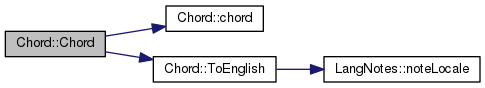
\includegraphics[width=350pt]{class_chord_ac61d5711e773d1d8203a6ee3d854142c_cgraph}
\end{center}
\end{figure}


\subsection{Member Function Documentation}
\mbox{\label{class_chord_adb32e210a420399a1ceffa3ad8f0dab7}} 
\index{Chord@{Chord}!chord@{chord}}
\index{chord@{chord}!Chord@{Chord}}
\subsubsection{chord()}
{\footnotesize\ttfamily Q\+String Chord\+::chord (\begin{DoxyParamCaption}{ }\end{DoxyParamCaption})}



chord 

\begin{DoxyReturn}{Returns}
the original name given in constructor 
\end{DoxyReturn}
Here is the caller graph for this function\+:
\nopagebreak
\begin{figure}[H]
\begin{center}
\leavevmode
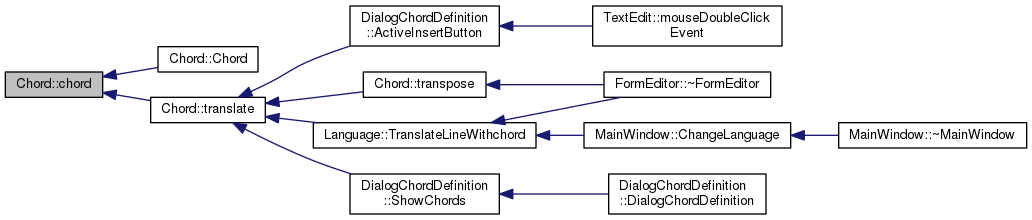
\includegraphics[width=350pt]{class_chord_adb32e210a420399a1ceffa3ad8f0dab7_icgraph}
\end{center}
\end{figure}
\mbox{\label{class_chord_a050ab41985c8a9895e108379d811f604}} 
\index{Chord@{Chord}!down@{down}}
\index{down@{down}!Chord@{Chord}}
\subsubsection{down()}
{\footnotesize\ttfamily Q\+String Chord\+::down (\begin{DoxyParamCaption}{ }\end{DoxyParamCaption})}



down the name of the chord on tne previous fret 

\begin{DoxyReturn}{Returns}

\end{DoxyReturn}
Here is the caller graph for this function\+:
\nopagebreak
\begin{figure}[H]
\begin{center}
\leavevmode
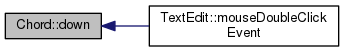
\includegraphics[width=330pt]{class_chord_a050ab41985c8a9895e108379d811f604_icgraph}
\end{center}
\end{figure}
\mbox{\label{class_chord_a168ef9c9f97eb6a37d2adfc451b0adf9}} 
\index{Chord@{Chord}!fret@{fret}}
\index{fret@{fret}!Chord@{Chord}}
\subsubsection{fret()}
{\footnotesize\ttfamily Q\+String Chord\+::fret (\begin{DoxyParamCaption}{ }\end{DoxyParamCaption})}



fret 

\begin{DoxyReturn}{Returns}
fret number \+: 0 1 etc... 
\end{DoxyReturn}
Here is the caller graph for this function\+:
\nopagebreak
\begin{figure}[H]
\begin{center}
\leavevmode
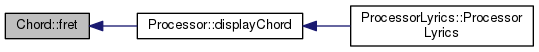
\includegraphics[width=350pt]{class_chord_a168ef9c9f97eb6a37d2adfc451b0adf9_icgraph}
\end{center}
\end{figure}
\mbox{\label{class_chord_a77af1b87e77e540cb48ed29a1ff8079f}} 
\index{Chord@{Chord}!name\+English@{name\+English}}
\index{name\+English@{name\+English}!Chord@{Chord}}
\subsubsection{name\+English()}
{\footnotesize\ttfamily Q\+String Chord\+::name\+English (\begin{DoxyParamCaption}{ }\end{DoxyParamCaption})}



name\+English 

\begin{DoxyReturn}{Returns}
the english chord name 
\end{DoxyReturn}
\mbox{\label{class_chord_a2f6e790c26dde21eb22f0500c7593b6a}} 
\index{Chord@{Chord}!name\+Locale@{name\+Locale}}
\index{name\+Locale@{name\+Locale}!Chord@{Chord}}
\subsubsection{name\+Locale()}
{\footnotesize\ttfamily Q\+String Chord\+::name\+Locale (\begin{DoxyParamCaption}{ }\end{DoxyParamCaption})}



name\+Locale 

\begin{DoxyReturn}{Returns}
the locale chord name 
\end{DoxyReturn}
Here is the caller graph for this function\+:
\nopagebreak
\begin{figure}[H]
\begin{center}
\leavevmode
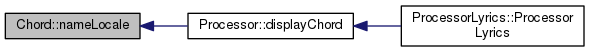
\includegraphics[width=350pt]{class_chord_a2f6e790c26dde21eb22f0500c7593b6a_icgraph}
\end{center}
\end{figure}
\mbox{\label{class_chord_a63e1e1b11f68987319ce657cefc537a1}} 
\index{Chord@{Chord}!nb\+Bar@{nb\+Bar}}
\index{nb\+Bar@{nb\+Bar}!Chord@{Chord}}
\subsubsection{nb\+Bar()}
{\footnotesize\ttfamily int Chord\+::nb\+Bar (\begin{DoxyParamCaption}{ }\end{DoxyParamCaption})}



nb\+Bar 

\begin{DoxyReturn}{Returns}
the number after the x 
\end{DoxyReturn}
\mbox{\label{class_chord_aa567ff9785ed505138a28926e8d5c608}} 
\index{Chord@{Chord}!nb\+Beat@{nb\+Beat}}
\index{nb\+Beat@{nb\+Beat}!Chord@{Chord}}
\subsubsection{nb\+Beat()}
{\footnotesize\ttfamily int Chord\+::nb\+Beat (\begin{DoxyParamCaption}{ }\end{DoxyParamCaption})}



nb\+Beat 

\begin{DoxyReturn}{Returns}
the number after the \+: 
\end{DoxyReturn}
\mbox{\label{class_chord_ac327ecc38a5359f06dab03b874120987}} 
\index{Chord@{Chord}!pure\+Name\+English@{pure\+Name\+English}}
\index{pure\+Name\+English@{pure\+Name\+English}!Chord@{Chord}}
\subsubsection{pure\+Name\+English()}
{\footnotesize\ttfamily Q\+String Chord\+::pure\+Name\+English (\begin{DoxyParamCaption}{ }\end{DoxyParamCaption})}



pure\+Name\+English 

\begin{DoxyReturn}{Returns}
same as name\+Locale but without beat, bar and degre D7(\+V)x2 become Re7 
\end{DoxyReturn}
Here is the caller graph for this function\+:
\nopagebreak
\begin{figure}[H]
\begin{center}
\leavevmode
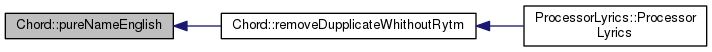
\includegraphics[width=350pt]{class_chord_ac327ecc38a5359f06dab03b874120987_icgraph}
\end{center}
\end{figure}
\mbox{\label{class_chord_aec2d95d7b27de1aed99c4e7fde68b9e0}} 
\index{Chord@{Chord}!pure\+Name\+Locale@{pure\+Name\+Locale}}
\index{pure\+Name\+Locale@{pure\+Name\+Locale}!Chord@{Chord}}
\subsubsection{pure\+Name\+Locale()}
{\footnotesize\ttfamily Q\+String Chord\+::pure\+Name\+Locale (\begin{DoxyParamCaption}{ }\end{DoxyParamCaption})}



pure\+Name\+Locale 

\begin{DoxyReturn}{Returns}

\end{DoxyReturn}
Here is the caller graph for this function\+:
\nopagebreak
\begin{figure}[H]
\begin{center}
\leavevmode
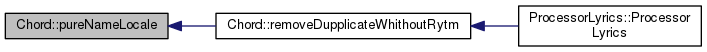
\includegraphics[width=350pt]{class_chord_aec2d95d7b27de1aed99c4e7fde68b9e0_icgraph}
\end{center}
\end{figure}
\mbox{\label{class_chord_ac5b55bda5f701f89695918c19e8caadc}} 
\index{Chord@{Chord}!remove\+Dupplicate\+Whithout\+Rytm@{remove\+Dupplicate\+Whithout\+Rytm}}
\index{remove\+Dupplicate\+Whithout\+Rytm@{remove\+Dupplicate\+Whithout\+Rytm}!Chord@{Chord}}
\subsubsection{remove\+Dupplicate\+Whithout\+Rytm()}
{\footnotesize\ttfamily Q\+String\+List Chord\+::remove\+Dupplicate\+Whithout\+Rytm (\begin{DoxyParamCaption}\item[{Q\+String\+List}]{chords,  }\item[{Q\+String}]{codelang }\end{DoxyParamCaption})\hspace{0.3cm}{\ttfamily [static]}}



remove\+Dupplicate\+Whithout\+Rytm 


\begin{DoxyParams}{Parameters}
{\em chords} & list of names of chord \\
\hline
{\em codelang} & \+: en,fr ... \\
\hline
\end{DoxyParams}
\begin{DoxyReturn}{Returns}
\+: suppress the dupplicate chords after removing the \+:2 x2 
\end{DoxyReturn}
Here is the call graph for this function\+:
\nopagebreak
\begin{figure}[H]
\begin{center}
\leavevmode
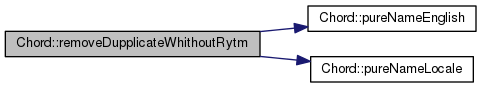
\includegraphics[width=350pt]{class_chord_ac5b55bda5f701f89695918c19e8caadc_cgraph}
\end{center}
\end{figure}
Here is the caller graph for this function\+:
\nopagebreak
\begin{figure}[H]
\begin{center}
\leavevmode
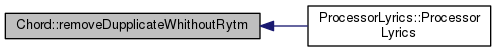
\includegraphics[width=350pt]{class_chord_ac5b55bda5f701f89695918c19e8caadc_icgraph}
\end{center}
\end{figure}
\mbox{\label{class_chord_ae9137152a3c9c3ac2e4f4dec85957d32}} 
\index{Chord@{Chord}!remove\+Rytm@{remove\+Rytm}}
\index{remove\+Rytm@{remove\+Rytm}!Chord@{Chord}}
\subsubsection{remove\+Rytm()}
{\footnotesize\ttfamily Q\+String Chord\+::remove\+Rytm (\begin{DoxyParamCaption}{ }\end{DoxyParamCaption})}



remove\+Rytm 

\begin{DoxyReturn}{Returns}
the name of the chord without \+:2 or x2 and translated in locale 
\end{DoxyReturn}
\mbox{\label{class_chord_ab54e7ef5f62c8e872a59ed5d8a8b68d8}} 
\index{Chord@{Chord}!To\+English@{To\+English}}
\index{To\+English@{To\+English}!Chord@{Chord}}
\subsubsection{To\+English()}
{\footnotesize\ttfamily Q\+String Chord\+::\+To\+English (\begin{DoxyParamCaption}\item[{Q\+String}]{chord }\end{DoxyParamCaption})}



To\+English. 


\begin{DoxyParams}{Parameters}
{\em chord} & in locale \\
\hline
\end{DoxyParams}
\begin{DoxyReturn}{Returns}
the chord name translated 
\end{DoxyReturn}
Here is the call graph for this function\+:
\nopagebreak
\begin{figure}[H]
\begin{center}
\leavevmode
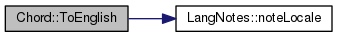
\includegraphics[width=325pt]{class_chord_ab54e7ef5f62c8e872a59ed5d8a8b68d8_cgraph}
\end{center}
\end{figure}
Here is the caller graph for this function\+:
\nopagebreak
\begin{figure}[H]
\begin{center}
\leavevmode
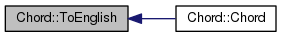
\includegraphics[width=283pt]{class_chord_ab54e7ef5f62c8e872a59ed5d8a8b68d8_icgraph}
\end{center}
\end{figure}
\mbox{\label{class_chord_ae5f32095442d1a7cf07251a29b0575b4}} 
\index{Chord@{Chord}!to\+Strings@{to\+Strings}}
\index{to\+Strings@{to\+Strings}!Chord@{Chord}}
\subsubsection{to\+Strings()}
{\footnotesize\ttfamily Q\+String\+List Chord\+::to\+Strings (\begin{DoxyParamCaption}{ }\end{DoxyParamCaption})}



to\+Strings 

\begin{DoxyReturn}{Returns}
the chords on string for example x x 0 2 1 2 
\end{DoxyReturn}
Here is the caller graph for this function\+:
\nopagebreak
\begin{figure}[H]
\begin{center}
\leavevmode
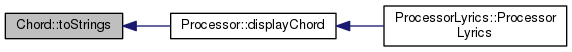
\includegraphics[width=350pt]{class_chord_ae5f32095442d1a7cf07251a29b0575b4_icgraph}
\end{center}
\end{figure}
\mbox{\label{class_chord_ad68a4f58d3dd18f09ea9bf7536e89284}} 
\index{Chord@{Chord}!translate@{translate}}
\index{translate@{translate}!Chord@{Chord}}
\subsubsection{translate()}
{\footnotesize\ttfamily Q\+String Chord\+::translate (\begin{DoxyParamCaption}\item[{Q\+String}]{chord,  }\item[{Q\+String}]{codelangfrom,  }\item[{Q\+String}]{minfrom,  }\item[{Q\+String}]{codelangto,  }\item[{Q\+String}]{minto }\end{DoxyParamCaption})\hspace{0.3cm}{\ttfamily [static]}}



translate 


\begin{DoxyParams}{Parameters}
{\em chord} & \+: a chord name \\
\hline
{\em codelangfrom} & \+: code from language \+: fr or en \\
\hline
{\em minfrom} & \+: symbol for minor \+: m or -\/ \\
\hline
{\em codelangto} & \+: code for language \+: fr or en \\
\hline
{\em minto} & \+: symbol for minor \+: for example m \\
\hline
\end{DoxyParams}
\begin{DoxyReturn}{Returns}
the chord translated 
\end{DoxyReturn}
Here is the call graph for this function\+:
\nopagebreak
\begin{figure}[H]
\begin{center}
\leavevmode
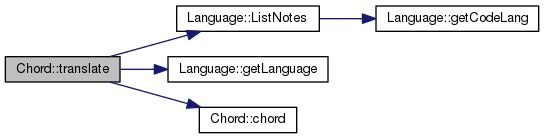
\includegraphics[width=350pt]{class_chord_ad68a4f58d3dd18f09ea9bf7536e89284_cgraph}
\end{center}
\end{figure}
Here is the caller graph for this function\+:
\nopagebreak
\begin{figure}[H]
\begin{center}
\leavevmode
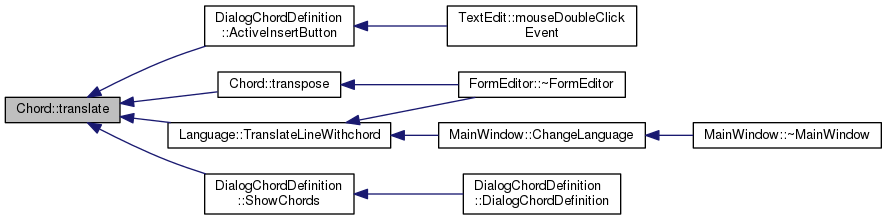
\includegraphics[width=350pt]{class_chord_ad68a4f58d3dd18f09ea9bf7536e89284_icgraph}
\end{center}
\end{figure}
\mbox{\label{class_chord_ac9f58e7a65e814970f69365dd3f5f2f9}} 
\index{Chord@{Chord}!transpose@{transpose}}
\index{transpose@{transpose}!Chord@{Chord}}
\subsubsection{transpose()}
{\footnotesize\ttfamily Q\+String Chord\+::transpose (\begin{DoxyParamCaption}\item[{int}]{degre,  }\item[{bool}]{parentheses,  }\item[{Q\+String}]{minfrom,  }\item[{Q\+String}]{minto }\end{DoxyParamCaption})}



transpose \+: transpose a chord 


\begin{DoxyParams}{Parameters}
{\em degre} & \+: number of fret \\
\hline
{\em parentheses} & \+: true of false \+: false you will not get the fret \\
\hline
{\em minfrom} & \+: minor symbol from \\
\hline
{\em minto} & \+: minor symbol to \\
\hline
\end{DoxyParams}
\begin{DoxyReturn}{Returns}
\+: the transposed chord 
\end{DoxyReturn}
Here is the call graph for this function\+:
\nopagebreak
\begin{figure}[H]
\begin{center}
\leavevmode
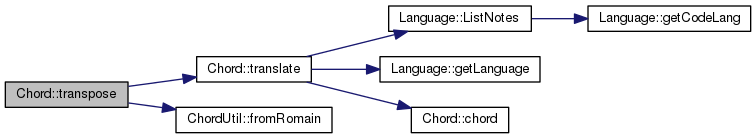
\includegraphics[width=350pt]{class_chord_ac9f58e7a65e814970f69365dd3f5f2f9_cgraph}
\end{center}
\end{figure}
Here is the caller graph for this function\+:
\nopagebreak
\begin{figure}[H]
\begin{center}
\leavevmode
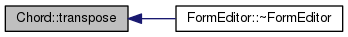
\includegraphics[width=333pt]{class_chord_ac9f58e7a65e814970f69365dd3f5f2f9_icgraph}
\end{center}
\end{figure}
\mbox{\label{class_chord_a67abd19a0206c062752eca1190db9280}} 
\index{Chord@{Chord}!up@{up}}
\index{up@{up}!Chord@{Chord}}
\subsubsection{up()}
{\footnotesize\ttfamily Q\+String Chord\+::up (\begin{DoxyParamCaption}{ }\end{DoxyParamCaption})}



up the name of the chord on the next fret 

\begin{DoxyReturn}{Returns}

\end{DoxyReturn}
Here is the caller graph for this function\+:
\nopagebreak
\begin{figure}[H]
\begin{center}
\leavevmode
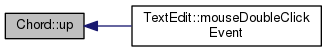
\includegraphics[width=317pt]{class_chord_a67abd19a0206c062752eca1190db9280_icgraph}
\end{center}
\end{figure}


The documentation for this class was generated from the following files\+:\begin{DoxyCompactItemize}
\item 
src/\textbf{ chord.\+h}\item 
src/\textbf{ chord.\+cpp}\end{DoxyCompactItemize}

\section{Chord\+Config Class Reference}
\label{class_chord_config}\index{Chord\+Config@{Chord\+Config}}


{\ttfamily \#include $<$chordconfig.\+h$>$}



Inheritance diagram for Chord\+Config\+:\nopagebreak
\begin{figure}[H]
\begin{center}
\leavevmode
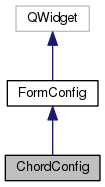
\includegraphics[width=151pt]{class_chord_config__inherit__graph}
\end{center}
\end{figure}


Collaboration diagram for Chord\+Config\+:\nopagebreak
\begin{figure}[H]
\begin{center}
\leavevmode
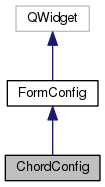
\includegraphics[width=151pt]{class_chord_config__coll__graph}
\end{center}
\end{figure}
\subsection*{Public Member Functions}
\begin{DoxyCompactItemize}
\item 
\textbf{ Chord\+Config} (Q\+Widget $\ast$parent=0)
\end{DoxyCompactItemize}
\subsection*{Additional Inherited Members}


\subsection{Constructor \& Destructor Documentation}
\mbox{\label{class_chord_config_a650f5c9d66d1c5e8a86c376b58dd0232}} 
\index{Chord\+Config@{Chord\+Config}!Chord\+Config@{Chord\+Config}}
\index{Chord\+Config@{Chord\+Config}!Chord\+Config@{Chord\+Config}}
\subsubsection{Chord\+Config()}
{\footnotesize\ttfamily Chord\+Config\+::\+Chord\+Config (\begin{DoxyParamCaption}\item[{Q\+Widget $\ast$}]{parent = {\ttfamily 0} }\end{DoxyParamCaption})}

Here is the call graph for this function\+:\nopagebreak
\begin{figure}[H]
\begin{center}
\leavevmode
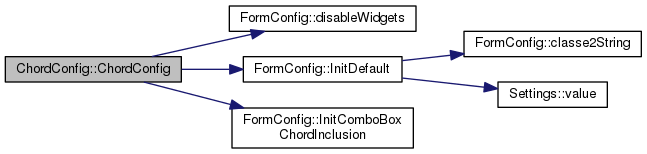
\includegraphics[width=350pt]{class_chord_config_a650f5c9d66d1c5e8a86c376b58dd0232_cgraph}
\end{center}
\end{figure}


The documentation for this class was generated from the following files\+:\begin{DoxyCompactItemize}
\item 
src/\textbf{ chordconfig.\+h}\item 
src/\textbf{ chordconfig.\+cpp}\end{DoxyCompactItemize}

\section{Chord\+Detector Class Reference}
\label{class_chord_detector}\index{Chord\+Detector@{Chord\+Detector}}


The \doxyref{Chord\+Detector}{p.}{class_chord_detector} class allow to detect a chord from list\+Notes. It is used on guitar neck to transform a list of notes to Q\+String\+List of chords given by the method \doxyref{detect\+Chord()}{p.}{class_chord_detector_a1d17c7c43eadf715a10a2910a5593fae}; The list of notes given to constructor are for example A, E, F The algorythm is given buy the tblscitype of the ChordV database. The ChordV Database containes two tables \+: tblscitype and Chords.  




{\ttfamily \#include $<$Chord\+Detector.\+h$>$}

\subsection*{Public Member Functions}
\begin{DoxyCompactItemize}
\item 
\textbf{ Chord\+Detector} (Q\+String\+List list\+Notes)
\begin{DoxyCompactList}\small\item\em \doxyref{Chord\+Detector}{p.}{class_chord_detector} the constuctor is called with list of notes given as a Q\+String\+List, for example A,E,F. \end{DoxyCompactList}\item 
Q\+String\+List \textbf{ detect\+Chord} ()
\begin{DoxyCompactList}\small\item\em detect\+Chord return the list of chord found. \end{DoxyCompactList}\end{DoxyCompactItemize}


\subsection{Detailed Description}
The \doxyref{Chord\+Detector}{p.}{class_chord_detector} class allow to detect a chord from list\+Notes. It is used on guitar neck to transform a list of notes to Q\+String\+List of chords given by the method \doxyref{detect\+Chord()}{p.}{class_chord_detector_a1d17c7c43eadf715a10a2910a5593fae}; The list of notes given to constructor are for example A, E, F The algorythm is given buy the tblscitype of the ChordV database. The ChordV Database containes two tables \+: tblscitype and Chords. 


\begin{DoxyItemize}
\item {\bfseries tblscitype} allows ot find txtcode of chord from interval
\item {\bfseries chords} keep chords with A7(\+I\+V) or A6 notation and the correspondance 4212222 or 0x02020 
\end{DoxyItemize}

\subsection{Constructor \& Destructor Documentation}
\mbox{\label{class_chord_detector_a19b59759dfae96b2a24ffa7b97869b62}} 
\index{Chord\+Detector@{Chord\+Detector}!Chord\+Detector@{Chord\+Detector}}
\index{Chord\+Detector@{Chord\+Detector}!Chord\+Detector@{Chord\+Detector}}
\subsubsection{Chord\+Detector()}
{\footnotesize\ttfamily Chord\+Detector\+::\+Chord\+Detector (\begin{DoxyParamCaption}\item[{Q\+String\+List}]{list\+Notes }\end{DoxyParamCaption})}



\doxyref{Chord\+Detector}{p.}{class_chord_detector} the constuctor is called with list of notes given as a Q\+String\+List, for example A,E,F. 


\begin{DoxyParams}{Parameters}
{\em list\+Notes} & \+: Q\+String\+List with all notes found on the neck. Th duplicated notes are removed. \\
\hline
\end{DoxyParams}


\subsection{Member Function Documentation}
\mbox{\label{class_chord_detector_a1d17c7c43eadf715a10a2910a5593fae}} 
\index{Chord\+Detector@{Chord\+Detector}!detect\+Chord@{detect\+Chord}}
\index{detect\+Chord@{detect\+Chord}!Chord\+Detector@{Chord\+Detector}}
\subsubsection{detect\+Chord()}
{\footnotesize\ttfamily Q\+String\+List Chord\+Detector\+::detect\+Chord (\begin{DoxyParamCaption}{ }\end{DoxyParamCaption})}



detect\+Chord return the list of chord found. 

\begin{DoxyReturn}{Returns}

\end{DoxyReturn}
Here is the caller graph for this function\+:\nopagebreak
\begin{figure}[H]
\begin{center}
\leavevmode
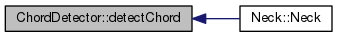
\includegraphics[width=325pt]{class_chord_detector_a1d17c7c43eadf715a10a2910a5593fae_icgraph}
\end{center}
\end{figure}


The documentation for this class was generated from the following files\+:\begin{DoxyCompactItemize}
\item 
src/\textbf{ Chord\+Detector.\+h}\item 
src/\textbf{ Chord\+Detector.\+cpp}\end{DoxyCompactItemize}

\section{Chord\+Diagram Class Reference}
\label{class_chord_diagram}\index{Chord\+Diagram@{Chord\+Diagram}}


The \doxyref{Chord\+Diagram}{p.}{class_chord_diagram} class is a widget class usable in designer to show chords in Qtt Designer.  




{\ttfamily \#include $<$chorddiagram.\+h$>$}



Inheritance diagram for Chord\+Diagram\+:\nopagebreak
\begin{figure}[H]
\begin{center}
\leavevmode
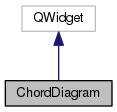
\includegraphics[width=160pt]{class_chord_diagram__inherit__graph}
\end{center}
\end{figure}


Collaboration diagram for Chord\+Diagram\+:\nopagebreak
\begin{figure}[H]
\begin{center}
\leavevmode
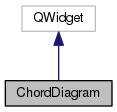
\includegraphics[width=160pt]{class_chord_diagram__coll__graph}
\end{center}
\end{figure}
\subsection*{Public Member Functions}
\begin{DoxyCompactItemize}
\item 
\textbf{ Chord\+Diagram} (Q\+Widget $\ast$parent=0)
\begin{DoxyCompactList}\small\item\em \doxyref{Chord\+Diagram}{p.}{class_chord_diagram} the constructor with Q\+Widget $\ast$parent who give the parent widget compliant to Graphic Designer of Qt\+Creator. \end{DoxyCompactList}\item 
void \textbf{ set\+Diagram} (Q\+String diagram)
\begin{DoxyCompactList}\small\item\em set\+Diagram when Widget is positionned give the name of the chord. \end{DoxyCompactList}\item 
Q\+String \textbf{ get\+Diagram} ()
\begin{DoxyCompactList}\small\item\em get\+Diagram return the diagram name in 52x122x form \end{DoxyCompactList}\end{DoxyCompactItemize}


\subsection{Detailed Description}
The \doxyref{Chord\+Diagram}{p.}{class_chord_diagram} class is a widget class usable in designer to show chords in Qtt Designer. 

\subsection{Constructor \& Destructor Documentation}
\mbox{\label{class_chord_diagram_a76f2ebbcfcefb985738e5428591f1f40}} 
\index{Chord\+Diagram@{Chord\+Diagram}!Chord\+Diagram@{Chord\+Diagram}}
\index{Chord\+Diagram@{Chord\+Diagram}!Chord\+Diagram@{Chord\+Diagram}}
\subsubsection{Chord\+Diagram()}
{\footnotesize\ttfamily Chord\+Diagram\+::\+Chord\+Diagram (\begin{DoxyParamCaption}\item[{Q\+Widget $\ast$}]{parent = {\ttfamily 0} }\end{DoxyParamCaption})\hspace{0.3cm}{\ttfamily [explicit]}}



\doxyref{Chord\+Diagram}{p.}{class_chord_diagram} the constructor with Q\+Widget $\ast$parent who give the parent widget compliant to Graphic Designer of Qt\+Creator. 


\begin{DoxyParams}{Parameters}
{\em parent} & \+: pointer on the parent \\
\hline
\end{DoxyParams}


\subsection{Member Function Documentation}
\mbox{\label{class_chord_diagram_abf346142ad2d712c352c03ce572a9fe0}} 
\index{Chord\+Diagram@{Chord\+Diagram}!get\+Diagram@{get\+Diagram}}
\index{get\+Diagram@{get\+Diagram}!Chord\+Diagram@{Chord\+Diagram}}
\subsubsection{get\+Diagram()}
{\footnotesize\ttfamily Q\+String Chord\+Diagram\+::get\+Diagram (\begin{DoxyParamCaption}{ }\end{DoxyParamCaption})}



get\+Diagram return the diagram name in 52x122x form 

\begin{DoxyReturn}{Returns}

\end{DoxyReturn}
\mbox{\label{class_chord_diagram_aaac87b71414b96ac3b6a6900fc5c0b07}} 
\index{Chord\+Diagram@{Chord\+Diagram}!set\+Diagram@{set\+Diagram}}
\index{set\+Diagram@{set\+Diagram}!Chord\+Diagram@{Chord\+Diagram}}
\subsubsection{set\+Diagram()}
{\footnotesize\ttfamily void Chord\+Diagram\+::set\+Diagram (\begin{DoxyParamCaption}\item[{Q\+String}]{diagram }\end{DoxyParamCaption})}



set\+Diagram when Widget is positionned give the name of the chord. 


\begin{DoxyParams}{Parameters}
{\em diagram} & is given in 52x122x form \\
\hline
\end{DoxyParams}


The documentation for this class was generated from the following files\+:\begin{DoxyCompactItemize}
\item 
src/\textbf{ chorddiagram.\+h}\item 
src/\textbf{ chorddiagram.\+cpp}\end{DoxyCompactItemize}

\section{Chord\+Util Class Reference}
\label{class_chord_util}\index{Chord\+Util@{Chord\+Util}}


Some utilities.  




{\ttfamily \#include $<$chordutil.\+h$>$}

\subsection*{Static Public Member Functions}
\begin{DoxyCompactItemize}
\item 
static Q\+String\+List \textbf{ Last\+Projects} ()
\begin{DoxyCompactList}\small\item\em Last\+Projects give the list of last\+Projects used to add in \doxyref{Main\+Window}{p.}{class_main_window} the list of last project opened. The list is stored in Q\+Settings. \end{DoxyCompactList}\item 
static void \textbf{ Memorize\+Project} (Q\+String filename)
\begin{DoxyCompactList}\small\item\em Memorize\+Project when we add a new project save the last 10 projects ( if 10 is the number of project stored). If the project is contained in the list, all the project are stored, if the given project is new, the older will be removed. \end{DoxyCompactList}\item 
static Q\+String \textbf{ get\+Last\+Directory} ()
\begin{DoxyCompactList}\small\item\em get\+Last\+Directory retrieve the name of the last directory opened. It is useful to memorize the last directory open by user in Q\+File\+Fialog or other. \end{DoxyCompactList}\item 
static void \textbf{ set\+Last\+Directory} (Q\+String filename)
\begin{DoxyCompactList}\small\item\em set\+Last\+Directory set the last directory opened. See \doxyref{get\+Last\+Directory()}{p.}{class_chord_util_abeb08c9c5ca31ea82eda4fca8ee791ff} \end{DoxyCompactList}\item 
static Q\+String \textbf{ to\+Romain} (int i)
\begin{DoxyCompactList}\small\item\em to\+Romain convert 1 to I, 5 to V, 9 to IX \end{DoxyCompactList}\item 
static Q\+String\+List \textbf{ Normalize} (Q\+String\+List Fret\+And6\+Strings)
\begin{DoxyCompactList}\small\item\em Normalize old fonction for compatubility ( Obsolete) \end{DoxyCompactList}\item 
static int \textbf{ from\+Romain} (Q\+String i)
\begin{DoxyCompactList}\small\item\em from\+Romain convert from I to 1, from V to 5, from IX to 9 \end{DoxyCompactList}\end{DoxyCompactItemize}


\subsection{Detailed Description}
Some utilities. 

The \doxyref{Chord\+Util}{p.}{class_chord_util} class a set of static function given information 

\subsection{Member Function Documentation}
\mbox{\label{class_chord_util_a0dbc0ac64daf39840647ac3607b96c7c}} 
\index{Chord\+Util@{Chord\+Util}!from\+Romain@{from\+Romain}}
\index{from\+Romain@{from\+Romain}!Chord\+Util@{Chord\+Util}}
\subsubsection{from\+Romain()}
{\footnotesize\ttfamily int Chord\+Util\+::from\+Romain (\begin{DoxyParamCaption}\item[{Q\+String}]{i }\end{DoxyParamCaption})\hspace{0.3cm}{\ttfamily [static]}}



from\+Romain convert from I to 1, from V to 5, from IX to 9 


\begin{DoxyParams}{Parameters}
{\em i} & \+: Q\+String of value in romain notation \\
\hline
\end{DoxyParams}
\begin{DoxyReturn}{Returns}
the value in integer 
\end{DoxyReturn}
Here is the caller graph for this function\+:
\nopagebreak
\begin{figure}[H]
\begin{center}
\leavevmode
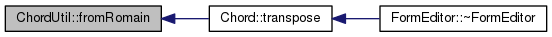
\includegraphics[width=350pt]{class_chord_util_a0dbc0ac64daf39840647ac3607b96c7c_icgraph}
\end{center}
\end{figure}
\mbox{\label{class_chord_util_abeb08c9c5ca31ea82eda4fca8ee791ff}} 
\index{Chord\+Util@{Chord\+Util}!get\+Last\+Directory@{get\+Last\+Directory}}
\index{get\+Last\+Directory@{get\+Last\+Directory}!Chord\+Util@{Chord\+Util}}
\subsubsection{get\+Last\+Directory()}
{\footnotesize\ttfamily Q\+String Chord\+Util\+::get\+Last\+Directory (\begin{DoxyParamCaption}{ }\end{DoxyParamCaption})\hspace{0.3cm}{\ttfamily [static]}}



get\+Last\+Directory retrieve the name of the last directory opened. It is useful to memorize the last directory open by user in Q\+File\+Fialog or other. 

\begin{DoxyReturn}{Returns}
\+: the name of the last directory opened 
\end{DoxyReturn}
Here is the caller graph for this function\+:
\nopagebreak
\begin{figure}[H]
\begin{center}
\leavevmode
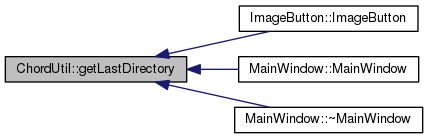
\includegraphics[width=350pt]{class_chord_util_abeb08c9c5ca31ea82eda4fca8ee791ff_icgraph}
\end{center}
\end{figure}
\mbox{\label{class_chord_util_a5e1db6203bf99d5e6c5a1cf262797b01}} 
\index{Chord\+Util@{Chord\+Util}!Last\+Projects@{Last\+Projects}}
\index{Last\+Projects@{Last\+Projects}!Chord\+Util@{Chord\+Util}}
\subsubsection{Last\+Projects()}
{\footnotesize\ttfamily Q\+String\+List Chord\+Util\+::\+Last\+Projects (\begin{DoxyParamCaption}{ }\end{DoxyParamCaption})\hspace{0.3cm}{\ttfamily [static]}}



Last\+Projects give the list of last\+Projects used to add in \doxyref{Main\+Window}{p.}{class_main_window} the list of last project opened. The list is stored in Q\+Settings. 

\begin{DoxyReturn}{Returns}
the Q\+String\+List with all the lastproject 
\end{DoxyReturn}
Here is the caller graph for this function\+:
\nopagebreak
\begin{figure}[H]
\begin{center}
\leavevmode
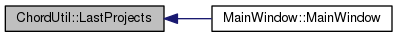
\includegraphics[width=350pt]{class_chord_util_a5e1db6203bf99d5e6c5a1cf262797b01_icgraph}
\end{center}
\end{figure}
\mbox{\label{class_chord_util_ad6bfac3dbeb2d7436f514ef709f01a21}} 
\index{Chord\+Util@{Chord\+Util}!Memorize\+Project@{Memorize\+Project}}
\index{Memorize\+Project@{Memorize\+Project}!Chord\+Util@{Chord\+Util}}
\subsubsection{Memorize\+Project()}
{\footnotesize\ttfamily void Chord\+Util\+::\+Memorize\+Project (\begin{DoxyParamCaption}\item[{Q\+String}]{filename }\end{DoxyParamCaption})\hspace{0.3cm}{\ttfamily [static]}}



Memorize\+Project when we add a new project save the last 10 projects ( if 10 is the number of project stored). If the project is contained in the list, all the project are stored, if the given project is new, the older will be removed. 


\begin{DoxyParams}{Parameters}
{\em filename} & the name of the new project \\
\hline
\end{DoxyParams}
Here is the caller graph for this function\+:
\nopagebreak
\begin{figure}[H]
\begin{center}
\leavevmode
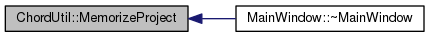
\includegraphics[width=350pt]{class_chord_util_ad6bfac3dbeb2d7436f514ef709f01a21_icgraph}
\end{center}
\end{figure}
\mbox{\label{class_chord_util_a70423579acb9825dd4318b176675541b}} 
\index{Chord\+Util@{Chord\+Util}!Normalize@{Normalize}}
\index{Normalize@{Normalize}!Chord\+Util@{Chord\+Util}}
\subsubsection{Normalize()}
{\footnotesize\ttfamily Q\+String\+List Chord\+Util\+::\+Normalize (\begin{DoxyParamCaption}\item[{Q\+String\+List}]{Fret\+And6\+Strings }\end{DoxyParamCaption})\hspace{0.3cm}{\ttfamily [static]}}



Normalize old fonction for compatubility ( Obsolete) 


\begin{DoxyParams}{Parameters}
{\em Fret\+And6\+Strings} & \\
\hline
\end{DoxyParams}
\begin{DoxyReturn}{Returns}

\end{DoxyReturn}
\mbox{\label{class_chord_util_a485337752434b4eb052b34af6f385f65}} 
\index{Chord\+Util@{Chord\+Util}!set\+Last\+Directory@{set\+Last\+Directory}}
\index{set\+Last\+Directory@{set\+Last\+Directory}!Chord\+Util@{Chord\+Util}}
\subsubsection{set\+Last\+Directory()}
{\footnotesize\ttfamily void Chord\+Util\+::set\+Last\+Directory (\begin{DoxyParamCaption}\item[{Q\+String}]{filename }\end{DoxyParamCaption})\hspace{0.3cm}{\ttfamily [static]}}



set\+Last\+Directory set the last directory opened. See \doxyref{get\+Last\+Directory()}{p.}{class_chord_util_abeb08c9c5ca31ea82eda4fca8ee791ff} 


\begin{DoxyParams}{Parameters}
{\em filename} & \+: the directory whe want to memorize \\
\hline
\end{DoxyParams}
Here is the caller graph for this function\+:
\nopagebreak
\begin{figure}[H]
\begin{center}
\leavevmode
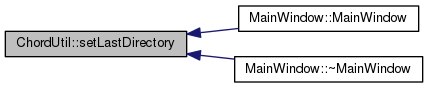
\includegraphics[width=350pt]{class_chord_util_a485337752434b4eb052b34af6f385f65_icgraph}
\end{center}
\end{figure}
\mbox{\label{class_chord_util_aed01d60e3f25c677cf420731dff07bdb}} 
\index{Chord\+Util@{Chord\+Util}!to\+Romain@{to\+Romain}}
\index{to\+Romain@{to\+Romain}!Chord\+Util@{Chord\+Util}}
\subsubsection{to\+Romain()}
{\footnotesize\ttfamily Q\+String Chord\+Util\+::to\+Romain (\begin{DoxyParamCaption}\item[{int}]{i }\end{DoxyParamCaption})\hspace{0.3cm}{\ttfamily [static]}}



to\+Romain convert 1 to I, 5 to V, 9 to IX 


\begin{DoxyParams}{Parameters}
{\em i} & \+: the integer value \\
\hline
\end{DoxyParams}
\begin{DoxyReturn}{Returns}
a string with romain notation 
\end{DoxyReturn}
Here is the caller graph for this function\+:
\nopagebreak
\begin{figure}[H]
\begin{center}
\leavevmode
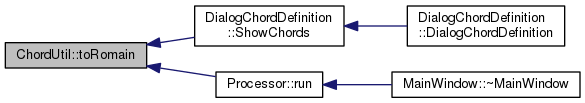
\includegraphics[width=350pt]{class_chord_util_aed01d60e3f25c677cf420731dff07bdb_icgraph}
\end{center}
\end{figure}


The documentation for this class was generated from the following files\+:\begin{DoxyCompactItemize}
\item 
src/\textbf{ chordutil.\+h}\item 
src/\textbf{ chordutil.\+cpp}\end{DoxyCompactItemize}

\section{Color\+Button Class Reference}
\label{class_color_button}\index{Color\+Button@{Color\+Button}}


The \doxyref{Color\+Button}{p.}{class_color_button} class allows to draw the color of Q\+Tool\+Button when user choose a color after click on button. The allow to show the color chooser by the button. This class is Qt\+Designer/\+Qt\+Creator complient.  




{\ttfamily \#include $<$colorbutton.\+h$>$}



Inheritance diagram for Color\+Button\+:\nopagebreak
\begin{figure}[H]
\begin{center}
\leavevmode
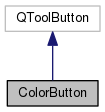
\includegraphics[width=151pt]{class_color_button__inherit__graph}
\end{center}
\end{figure}


Collaboration diagram for Color\+Button\+:\nopagebreak
\begin{figure}[H]
\begin{center}
\leavevmode
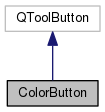
\includegraphics[width=151pt]{class_color_button__coll__graph}
\end{center}
\end{figure}
\subsection*{Signals}
\begin{DoxyCompactItemize}
\item 
void \textbf{ Color\+Changed} (Q\+Color color)
\end{DoxyCompactItemize}
\subsection*{Public Member Functions}
\begin{DoxyCompactItemize}
\item 
\textbf{ Color\+Button} (Q\+Widget $\ast$parent=0)
\begin{DoxyCompactList}\small\item\em \doxyref{Color\+Button}{p.}{class_color_button} construtor with the parent widget argument allowing to use in Qt\+Designer. \end{DoxyCompactList}\item 
Q\+Color \textbf{ get\+Color} ()
\begin{DoxyCompactList}\small\item\em get\+Color get the color of the button \end{DoxyCompactList}\item 
void \textbf{ set\+Color} (Q\+Color color)
\begin{DoxyCompactList}\small\item\em set\+Color set the color of the button \end{DoxyCompactList}\end{DoxyCompactItemize}


\subsection{Detailed Description}
The \doxyref{Color\+Button}{p.}{class_color_button} class allows to draw the color of Q\+Tool\+Button when user choose a color after click on button. The allow to show the color chooser by the button. This class is Qt\+Designer/\+Qt\+Creator complient. 

\subsection{Constructor \& Destructor Documentation}
\mbox{\label{class_color_button_a128b21900f22efdc9d71d0bffa0b64f8}} 
\index{Color\+Button@{Color\+Button}!Color\+Button@{Color\+Button}}
\index{Color\+Button@{Color\+Button}!Color\+Button@{Color\+Button}}
\subsubsection{Color\+Button()}
{\footnotesize\ttfamily Color\+Button\+::\+Color\+Button (\begin{DoxyParamCaption}\item[{Q\+Widget $\ast$}]{parent = {\ttfamily 0} }\end{DoxyParamCaption})}



\doxyref{Color\+Button}{p.}{class_color_button} construtor with the parent widget argument allowing to use in Qt\+Designer. 


\begin{DoxyParams}{Parameters}
{\em parent} & \+: the parent \\
\hline
\end{DoxyParams}
Here is the call graph for this function\+:\nopagebreak
\begin{figure}[H]
\begin{center}
\leavevmode
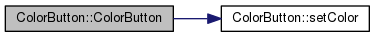
\includegraphics[width=350pt]{class_color_button_a128b21900f22efdc9d71d0bffa0b64f8_cgraph}
\end{center}
\end{figure}


\subsection{Member Function Documentation}
\mbox{\label{class_color_button_afeb98f603f62881e8f04a263be24c8b2}} 
\index{Color\+Button@{Color\+Button}!Color\+Changed@{Color\+Changed}}
\index{Color\+Changed@{Color\+Changed}!Color\+Button@{Color\+Button}}
\subsubsection{Color\+Changed}
{\footnotesize\ttfamily void Color\+Button\+::\+Color\+Changed (\begin{DoxyParamCaption}\item[{Q\+Color}]{color }\end{DoxyParamCaption})\hspace{0.3cm}{\ttfamily [signal]}}

Here is the caller graph for this function\+:\nopagebreak
\begin{figure}[H]
\begin{center}
\leavevmode
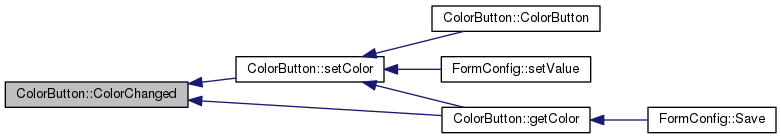
\includegraphics[width=350pt]{class_color_button_afeb98f603f62881e8f04a263be24c8b2_icgraph}
\end{center}
\end{figure}
\mbox{\label{class_color_button_ac849d69aa9efec941b3a0604820577bc}} 
\index{Color\+Button@{Color\+Button}!get\+Color@{get\+Color}}
\index{get\+Color@{get\+Color}!Color\+Button@{Color\+Button}}
\subsubsection{get\+Color()}
{\footnotesize\ttfamily Q\+Color Color\+Button\+::get\+Color (\begin{DoxyParamCaption}{ }\end{DoxyParamCaption})\hspace{0.3cm}{\ttfamily [inline]}}



get\+Color get the color of the button 

\begin{DoxyReturn}{Returns}
the color in Q\+Color type 
\end{DoxyReturn}
Here is the call graph for this function\+:\nopagebreak
\begin{figure}[H]
\begin{center}
\leavevmode
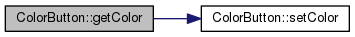
\includegraphics[width=338pt]{class_color_button_ac849d69aa9efec941b3a0604820577bc_cgraph}
\end{center}
\end{figure}
Here is the caller graph for this function\+:\nopagebreak
\begin{figure}[H]
\begin{center}
\leavevmode
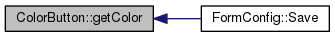
\includegraphics[width=323pt]{class_color_button_ac849d69aa9efec941b3a0604820577bc_icgraph}
\end{center}
\end{figure}
\mbox{\label{class_color_button_a2a564d30044197785035be7babfbf66b}} 
\index{Color\+Button@{Color\+Button}!set\+Color@{set\+Color}}
\index{set\+Color@{set\+Color}!Color\+Button@{Color\+Button}}
\subsubsection{set\+Color()}
{\footnotesize\ttfamily void Color\+Button\+::set\+Color (\begin{DoxyParamCaption}\item[{Q\+Color}]{color }\end{DoxyParamCaption})}



set\+Color set the color of the button 


\begin{DoxyParams}{Parameters}
{\em color} & giver with Q\+Color attribute \\
\hline
\end{DoxyParams}
Here is the caller graph for this function\+:\nopagebreak
\begin{figure}[H]
\begin{center}
\leavevmode
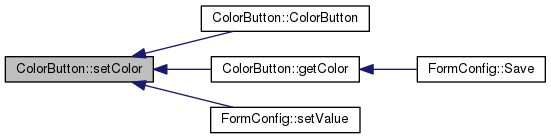
\includegraphics[width=350pt]{class_color_button_a2a564d30044197785035be7babfbf66b_icgraph}
\end{center}
\end{figure}


The documentation for this class was generated from the following files\+:\begin{DoxyCompactItemize}
\item 
src/\textbf{ colorbutton.\+h}\item 
src/\textbf{ colorbutton.\+cpp}\end{DoxyCompactItemize}

\section{Const Class Reference}
\label{class_const}\index{Const@{Const}}


The \doxyref{Const}{p.}{class_const} class set of constant classes.  




{\ttfamily \#include $<$const.\+h$>$}

\subsection*{Public Types}
\begin{DoxyCompactItemize}
\item 
enum \textbf{ Page\+Number} \{ \textbf{ No}, 
\textbf{ Center}, 
\textbf{ Outside}
 \}\begin{DoxyCompactList}\small\item\em The Page\+Number enum can be No for no pagnumber, Center ou Outside. \end{DoxyCompactList}
\item 
enum \textbf{ Plex} \{ \textbf{ Simplex}, 
\textbf{ Duplex}
 \}\begin{DoxyCompactList}\small\item\em The Plex enum can be Simplex it one side is printed, or Duplex if each page is printed. \end{DoxyCompactList}
\item 
enum \textbf{ Page\+Style} \{ \textbf{ Number}, 
\textbf{ Number\+And\+Tiret}, 
\textbf{ Number\+Divide\+By\+Page\+N\+Umber}, 
\textbf{ Number\+And\+Arrows}
 \}\begin{DoxyCompactList}\small\item\em The Page\+Style enum type of page number on button of each page Number is 1 Number and Tiret -\/ 1 -\/ Number\+Divide\+By\+Page\+N\+Umber 1/50 Number\+And\+Arrows $<$1$>$ \end{DoxyCompactList}
\end{DoxyCompactItemize}
\subsection*{Static Public Member Functions}
\begin{DoxyCompactItemize}
\item 
static \textbf{ Page\+Number} \textbf{ get\+Page\+Number} (int i)
\begin{DoxyCompactList}\small\item\em get\+Page\+Number return No Center or Outsde from 0 1 or 2 parameter \end{DoxyCompactList}\end{DoxyCompactItemize}


\subsection{Detailed Description}
The \doxyref{Const}{p.}{class_const} class set of constant classes. 

\subsection{Member Enumeration Documentation}
\mbox{\label{class_const_a33a65462824994bbfdbb64886718f8c9}} 
\index{Const@{Const}!Page\+Number@{Page\+Number}}
\index{Page\+Number@{Page\+Number}!Const@{Const}}
\subsubsection{Page\+Number}
{\footnotesize\ttfamily enum \textbf{ Const\+::\+Page\+Number}}



The Page\+Number enum can be No for no pagnumber, Center ou Outside. 

\begin{DoxyEnumFields}{Enumerator}
\raisebox{\heightof{T}}[0pt][0pt]{\index{No@{No}!Const@{Const}}\index{Const@{Const}!No@{No}}}\mbox{\label{class_const_a33a65462824994bbfdbb64886718f8c9a666f50edbd084b885c28cfc4b598a7ba}} 
No&\\
\hline

\raisebox{\heightof{T}}[0pt][0pt]{\index{Center@{Center}!Const@{Const}}\index{Const@{Const}!Center@{Center}}}\mbox{\label{class_const_a33a65462824994bbfdbb64886718f8c9a47bfa8b3cbbafc0e56a2078dda0e4eba}} 
Center&\\
\hline

\raisebox{\heightof{T}}[0pt][0pt]{\index{Outside@{Outside}!Const@{Const}}\index{Const@{Const}!Outside@{Outside}}}\mbox{\label{class_const_a33a65462824994bbfdbb64886718f8c9a12654e5371e65b0c95053ea0f3786986}} 
Outside&\\
\hline

\end{DoxyEnumFields}
\mbox{\label{class_const_a6a90969680fcb15ce73bcf5e1199c866}} 
\index{Const@{Const}!Page\+Style@{Page\+Style}}
\index{Page\+Style@{Page\+Style}!Const@{Const}}
\subsubsection{Page\+Style}
{\footnotesize\ttfamily enum \textbf{ Const\+::\+Page\+Style}}



The Page\+Style enum type of page number on button of each page Number is 1 Number and Tiret -\/ 1 -\/ Number\+Divide\+By\+Page\+N\+Umber 1/50 Number\+And\+Arrows $<$1$>$ 

\begin{DoxyEnumFields}{Enumerator}
\raisebox{\heightof{T}}[0pt][0pt]{\index{Number@{Number}!Const@{Const}}\index{Const@{Const}!Number@{Number}}}\mbox{\label{class_const_a6a90969680fcb15ce73bcf5e1199c866ad77dd5ec4b776cf53bc7dc0dbaf363e8}} 
Number&\\
\hline

\raisebox{\heightof{T}}[0pt][0pt]{\index{Number\+And\+Tiret@{Number\+And\+Tiret}!Const@{Const}}\index{Const@{Const}!Number\+And\+Tiret@{Number\+And\+Tiret}}}\mbox{\label{class_const_a6a90969680fcb15ce73bcf5e1199c866ae83769f7a1ab75d28fad1abab5597fe8}} 
Number\+And\+Tiret&\\
\hline

\raisebox{\heightof{T}}[0pt][0pt]{\index{Number\+Divide\+By\+Page\+N\+Umber@{Number\+Divide\+By\+Page\+N\+Umber}!Const@{Const}}\index{Const@{Const}!Number\+Divide\+By\+Page\+N\+Umber@{Number\+Divide\+By\+Page\+N\+Umber}}}\mbox{\label{class_const_a6a90969680fcb15ce73bcf5e1199c866a465c512f9b1f920a49bc90b1f8a022d5}} 
Number\+Divide\+By\+Page\+N\+Umber&\\
\hline

\raisebox{\heightof{T}}[0pt][0pt]{\index{Number\+And\+Arrows@{Number\+And\+Arrows}!Const@{Const}}\index{Const@{Const}!Number\+And\+Arrows@{Number\+And\+Arrows}}}\mbox{\label{class_const_a6a90969680fcb15ce73bcf5e1199c866a4bec5476e5ae2baf8a82b8287c4f7471}} 
Number\+And\+Arrows&\\
\hline

\end{DoxyEnumFields}
\mbox{\label{class_const_a196e014fb08ef59d4acb10e7ccf779b8}} 
\index{Const@{Const}!Plex@{Plex}}
\index{Plex@{Plex}!Const@{Const}}
\subsubsection{Plex}
{\footnotesize\ttfamily enum \textbf{ Const\+::\+Plex}}



The Plex enum can be Simplex it one side is printed, or Duplex if each page is printed. 

\begin{DoxyEnumFields}{Enumerator}
\raisebox{\heightof{T}}[0pt][0pt]{\index{Simplex@{Simplex}!Const@{Const}}\index{Const@{Const}!Simplex@{Simplex}}}\mbox{\label{class_const_a196e014fb08ef59d4acb10e7ccf779b8a8ec2a5f7136df9bc0a31dbf6fbf16e4e}} 
Simplex&\\
\hline

\raisebox{\heightof{T}}[0pt][0pt]{\index{Duplex@{Duplex}!Const@{Const}}\index{Const@{Const}!Duplex@{Duplex}}}\mbox{\label{class_const_a196e014fb08ef59d4acb10e7ccf779b8abbcdc11d6ef48747bd65d7f04757445c}} 
Duplex&\\
\hline

\end{DoxyEnumFields}


\subsection{Member Function Documentation}
\mbox{\label{class_const_a98e1b38ae4383cbf79afef6431e71332}} 
\index{Const@{Const}!get\+Page\+Number@{get\+Page\+Number}}
\index{get\+Page\+Number@{get\+Page\+Number}!Const@{Const}}
\subsubsection{get\+Page\+Number()}
{\footnotesize\ttfamily static \textbf{ Page\+Number} Const\+::get\+Page\+Number (\begin{DoxyParamCaption}\item[{int}]{i }\end{DoxyParamCaption})\hspace{0.3cm}{\ttfamily [inline]}, {\ttfamily [static]}}



get\+Page\+Number return No Center or Outsde from 0 1 or 2 parameter 


\begin{DoxyParams}{Parameters}
{\em i} & \\
\hline
\end{DoxyParams}
\begin{DoxyReturn}{Returns}

\end{DoxyReturn}
Here is the caller graph for this function\+:\nopagebreak
\begin{figure}[H]
\begin{center}
\leavevmode
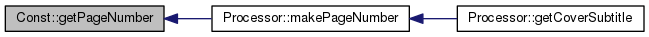
\includegraphics[width=350pt]{class_const_a98e1b38ae4383cbf79afef6431e71332_icgraph}
\end{center}
\end{figure}


The documentation for this class was generated from the following file\+:\begin{DoxyCompactItemize}
\item 
src/\textbf{ const.\+h}\end{DoxyCompactItemize}

\section{Dialog\+About Class Reference}
\label{class_dialog_about}\index{Dialog\+About@{Dialog\+About}}


The \doxyref{Dialog\+About}{p.}{class_dialog_about} class show the Dialog about.  




{\ttfamily \#include $<$dialogabout.\+h$>$}



Inheritance diagram for Dialog\+About\+:\nopagebreak
\begin{figure}[H]
\begin{center}
\leavevmode
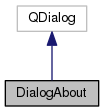
\includegraphics[width=150pt]{class_dialog_about__inherit__graph}
\end{center}
\end{figure}


Collaboration diagram for Dialog\+About\+:\nopagebreak
\begin{figure}[H]
\begin{center}
\leavevmode
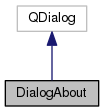
\includegraphics[width=150pt]{class_dialog_about__coll__graph}
\end{center}
\end{figure}
\subsection*{Public Member Functions}
\begin{DoxyCompactItemize}
\item 
\textbf{ Dialog\+About} (Q\+Widget $\ast$parent=0)
\begin{DoxyCompactList}\small\item\em \doxyref{Dialog\+About}{p.}{class_dialog_about} the constructor to show the About Dialog. \end{DoxyCompactList}\item 
\textbf{ $\sim$\+Dialog\+About} ()
\end{DoxyCompactItemize}


\subsection{Detailed Description}
The \doxyref{Dialog\+About}{p.}{class_dialog_about} class show the Dialog about. 

\subsection{Constructor \& Destructor Documentation}
\mbox{\label{class_dialog_about_a190b23e7ee6baf399a1a026c1a400e53}} 
\index{Dialog\+About@{Dialog\+About}!Dialog\+About@{Dialog\+About}}
\index{Dialog\+About@{Dialog\+About}!Dialog\+About@{Dialog\+About}}
\subsubsection{Dialog\+About()}
{\footnotesize\ttfamily Dialog\+About\+::\+Dialog\+About (\begin{DoxyParamCaption}\item[{Q\+Widget $\ast$}]{parent = {\ttfamily 0} }\end{DoxyParamCaption})\hspace{0.3cm}{\ttfamily [explicit]}}



\doxyref{Dialog\+About}{p.}{class_dialog_about} the constructor to show the About Dialog. 


\begin{DoxyParams}{Parameters}
{\em parent} & \\
\hline
\end{DoxyParams}
\mbox{\label{class_dialog_about_a0b141c358e2032f26464f7a4d85f4bd8}} 
\index{Dialog\+About@{Dialog\+About}!````~Dialog\+About@{$\sim$\+Dialog\+About}}
\index{````~Dialog\+About@{$\sim$\+Dialog\+About}!Dialog\+About@{Dialog\+About}}
\subsubsection{$\sim$\+Dialog\+About()}
{\footnotesize\ttfamily Dialog\+About\+::$\sim$\+Dialog\+About (\begin{DoxyParamCaption}{ }\end{DoxyParamCaption})}



The documentation for this class was generated from the following files\+:\begin{DoxyCompactItemize}
\item 
src/\textbf{ dialogabout.\+h}\item 
src/\textbf{ dialogabout.\+cpp}\end{DoxyCompactItemize}

\section{Dialog\+Bar Class Reference}
\label{class_dialog_bar}\index{Dialog\+Bar@{Dialog\+Bar}}


The \doxyref{Dialog\+Bar}{p.}{class_dialog_bar} class allow to choose the bar dialog for example 4/4 or 3/4 information.  




{\ttfamily \#include $<$dialogbar.\+h$>$}



Inheritance diagram for Dialog\+Bar\+:\nopagebreak
\begin{figure}[H]
\begin{center}
\leavevmode
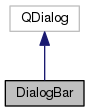
\includegraphics[width=139pt]{class_dialog_bar__inherit__graph}
\end{center}
\end{figure}


Collaboration diagram for Dialog\+Bar\+:\nopagebreak
\begin{figure}[H]
\begin{center}
\leavevmode
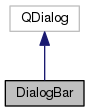
\includegraphics[width=139pt]{class_dialog_bar__coll__graph}
\end{center}
\end{figure}
\subsection*{Public Member Functions}
\begin{DoxyCompactItemize}
\item 
\textbf{ Dialog\+Bar} (Q\+Widget $\ast$parent=0)
\begin{DoxyCompactList}\small\item\em \doxyref{Dialog\+Bar}{p.}{class_dialog_bar} is complient with Qt\+Designer allowing to promote a widget to \doxyref{Dialog\+Bar}{p.}{class_dialog_bar}. \end{DoxyCompactList}\item 
\textbf{ $\sim$\+Dialog\+Bar} ()
\item 
bool \textbf{ canceled} ()
\begin{DoxyCompactList}\small\item\em canceled the dialog was canceled \end{DoxyCompactList}\item 
Q\+String \textbf{ value} ()
\begin{DoxyCompactList}\small\item\em return value like 4/4 or 3/4 \end{DoxyCompactList}\end{DoxyCompactItemize}


\subsection{Detailed Description}
The \doxyref{Dialog\+Bar}{p.}{class_dialog_bar} class allow to choose the bar dialog for example 4/4 or 3/4 information. 

\subsection{Constructor \& Destructor Documentation}
\mbox{\label{class_dialog_bar_a33b1b94db7bb611613b01b6e943aa0c3}} 
\index{Dialog\+Bar@{Dialog\+Bar}!Dialog\+Bar@{Dialog\+Bar}}
\index{Dialog\+Bar@{Dialog\+Bar}!Dialog\+Bar@{Dialog\+Bar}}
\subsubsection{Dialog\+Bar()}
{\footnotesize\ttfamily Dialog\+Bar\+::\+Dialog\+Bar (\begin{DoxyParamCaption}\item[{Q\+Widget $\ast$}]{parent = {\ttfamily 0} }\end{DoxyParamCaption})\hspace{0.3cm}{\ttfamily [explicit]}}



\doxyref{Dialog\+Bar}{p.}{class_dialog_bar} is complient with Qt\+Designer allowing to promote a widget to \doxyref{Dialog\+Bar}{p.}{class_dialog_bar}. 


\begin{DoxyParams}{Parameters}
{\em parent} & \\
\hline
\end{DoxyParams}
\mbox{\label{class_dialog_bar_a95a3d1bc5be26982c23cbbdaeabc00ef}} 
\index{Dialog\+Bar@{Dialog\+Bar}!````~Dialog\+Bar@{$\sim$\+Dialog\+Bar}}
\index{````~Dialog\+Bar@{$\sim$\+Dialog\+Bar}!Dialog\+Bar@{Dialog\+Bar}}
\subsubsection{$\sim$\+Dialog\+Bar()}
{\footnotesize\ttfamily Dialog\+Bar\+::$\sim$\+Dialog\+Bar (\begin{DoxyParamCaption}{ }\end{DoxyParamCaption})}



\subsection{Member Function Documentation}
\mbox{\label{class_dialog_bar_a40c3cce878287b420ca96df210b684dc}} 
\index{Dialog\+Bar@{Dialog\+Bar}!canceled@{canceled}}
\index{canceled@{canceled}!Dialog\+Bar@{Dialog\+Bar}}
\subsubsection{canceled()}
{\footnotesize\ttfamily bool Dialog\+Bar\+::canceled (\begin{DoxyParamCaption}{ }\end{DoxyParamCaption})}



canceled the dialog was canceled 

\begin{DoxyReturn}{Returns}

\end{DoxyReturn}
Here is the caller graph for this function\+:\nopagebreak
\begin{figure}[H]
\begin{center}
\leavevmode
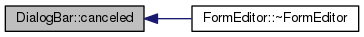
\includegraphics[width=345pt]{class_dialog_bar_a40c3cce878287b420ca96df210b684dc_icgraph}
\end{center}
\end{figure}
\mbox{\label{class_dialog_bar_ad2c63d251ea55533849837c9ec22ada1}} 
\index{Dialog\+Bar@{Dialog\+Bar}!value@{value}}
\index{value@{value}!Dialog\+Bar@{Dialog\+Bar}}
\subsubsection{value()}
{\footnotesize\ttfamily Q\+String Dialog\+Bar\+::value (\begin{DoxyParamCaption}{ }\end{DoxyParamCaption})}



return value like 4/4 or 3/4 

\begin{DoxyReturn}{Returns}
the Q\+String value returned 
\end{DoxyReturn}
Here is the caller graph for this function\+:\nopagebreak
\begin{figure}[H]
\begin{center}
\leavevmode
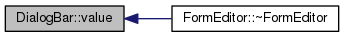
\includegraphics[width=330pt]{class_dialog_bar_ad2c63d251ea55533849837c9ec22ada1_icgraph}
\end{center}
\end{figure}


The documentation for this class was generated from the following files\+:\begin{DoxyCompactItemize}
\item 
src/\textbf{ dialogbar.\+h}\item 
src/\textbf{ dialogbar.\+cpp}\end{DoxyCompactItemize}

\section{Dialog\+Change\+Chord\+Name Class Reference}
\label{class_dialog_change_chord_name}\index{Dialog\+Change\+Chord\+Name@{Dialog\+Change\+Chord\+Name}}


The \doxyref{Dialog\+Change\+Chord\+Name}{p.}{class_dialog_change_chord_name} class used to change language of name of a chord by transposition.  




{\ttfamily \#include $<$dialogchangechordname.\+h$>$}



Inheritance diagram for Dialog\+Change\+Chord\+Name\+:\nopagebreak
\begin{figure}[H]
\begin{center}
\leavevmode
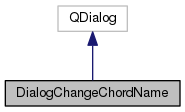
\includegraphics[width=211pt]{class_dialog_change_chord_name__inherit__graph}
\end{center}
\end{figure}


Collaboration diagram for Dialog\+Change\+Chord\+Name\+:\nopagebreak
\begin{figure}[H]
\begin{center}
\leavevmode
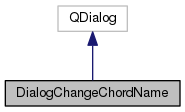
\includegraphics[width=211pt]{class_dialog_change_chord_name__coll__graph}
\end{center}
\end{figure}
\subsection*{Public Member Functions}
\begin{DoxyCompactItemize}
\item 
\textbf{ Dialog\+Change\+Chord\+Name} (Q\+Widget $\ast$parent=0)
\begin{DoxyCompactList}\small\item\em \doxyref{Dialog\+Change\+Chord\+Name}{p.}{class_dialog_change_chord_name} Dialog to Change chord Name \+: language or transposition. \end{DoxyCompactList}\item 
\textbf{ $\sim$\+Dialog\+Change\+Chord\+Name} ()
\item 
Q\+String \textbf{ get\+From\+Lang} ()
\begin{DoxyCompactList}\small\item\em get\+From\+Lang after change return from language \end{DoxyCompactList}\item 
Q\+String \textbf{ get\+To\+Lang} ()
\begin{DoxyCompactList}\small\item\em get\+To\+Lang after change return to language \end{DoxyCompactList}\item 
Q\+String \textbf{ get\+From\+Min} ()
\begin{DoxyCompactList}\small\item\em get\+From\+Min after change return Minor notation for from conversion. Exampele m or -\/ \end{DoxyCompactList}\item 
Q\+String \textbf{ get\+To\+Min} ()
\begin{DoxyCompactList}\small\item\em get\+To\+Min after change return Minor notation for to conversion. Exampele m or -\/ \end{DoxyCompactList}\item 
int \textbf{ get\+From\+Lang\+Index} ()
\begin{DoxyCompactList}\small\item\em get\+From\+Lang\+Index return index of From\+Lang combobox \end{DoxyCompactList}\item 
int \textbf{ get\+To\+Lang\+Index} ()
\begin{DoxyCompactList}\small\item\em get\+To\+Lang\+Index return index of To\+Lang Combobox \end{DoxyCompactList}\item 
int \textbf{ get\+To\+Min\+Index} ()
\begin{DoxyCompactList}\small\item\em get\+To\+Min\+Index return index of To\+Lang Combobox \end{DoxyCompactList}\item 
int \textbf{ get\+From\+Min\+Index} ()
\begin{DoxyCompactList}\small\item\em get\+From\+Min\+Index return index of From\+Lang Combobox \end{DoxyCompactList}\item 
void \textbf{ set\+From\+Lang} (int lang)
\begin{DoxyCompactList}\small\item\em set\+From\+Lang set the index of From\+Lang combobox \end{DoxyCompactList}\item 
void \textbf{ set\+To\+Lang} (int min)
\begin{DoxyCompactList}\small\item\em set\+To\+Lang set tje index of To\+From combobox \end{DoxyCompactList}\item 
void \textbf{ set\+From\+Min} (int lang)
\begin{DoxyCompactList}\small\item\em set\+From\+Min idem with Minor letter \end{DoxyCompactList}\item 
void \textbf{ set\+To\+Min} (int min)
\begin{DoxyCompactList}\small\item\em set\+To\+Min same as above with To record \end{DoxyCompactList}\item 
bool \textbf{ Ok\+Dialog} ()
\begin{DoxyCompactList}\small\item\em Ok\+Dialog the dialog return ok (true) or cancel(false) \end{DoxyCompactList}\end{DoxyCompactItemize}


\subsection{Detailed Description}
The \doxyref{Dialog\+Change\+Chord\+Name}{p.}{class_dialog_change_chord_name} class used to change language of name of a chord by transposition. 

\subsection{Constructor \& Destructor Documentation}
\mbox{\label{class_dialog_change_chord_name_aa59bf37f7c29daaa9a6cfe5f7cc2804d}} 
\index{Dialog\+Change\+Chord\+Name@{Dialog\+Change\+Chord\+Name}!Dialog\+Change\+Chord\+Name@{Dialog\+Change\+Chord\+Name}}
\index{Dialog\+Change\+Chord\+Name@{Dialog\+Change\+Chord\+Name}!Dialog\+Change\+Chord\+Name@{Dialog\+Change\+Chord\+Name}}
\subsubsection{Dialog\+Change\+Chord\+Name()}
{\footnotesize\ttfamily Dialog\+Change\+Chord\+Name\+::\+Dialog\+Change\+Chord\+Name (\begin{DoxyParamCaption}\item[{Q\+Widget $\ast$}]{parent = {\ttfamily 0} }\end{DoxyParamCaption})\hspace{0.3cm}{\ttfamily [explicit]}}



\doxyref{Dialog\+Change\+Chord\+Name}{p.}{class_dialog_change_chord_name} Dialog to Change chord Name \+: language or transposition. 


\begin{DoxyParams}{Parameters}
{\em parent} & \\
\hline
\end{DoxyParams}
\mbox{\label{class_dialog_change_chord_name_af48886d80f3dfa1d3240af94989868bd}} 
\index{Dialog\+Change\+Chord\+Name@{Dialog\+Change\+Chord\+Name}!````~Dialog\+Change\+Chord\+Name@{$\sim$\+Dialog\+Change\+Chord\+Name}}
\index{````~Dialog\+Change\+Chord\+Name@{$\sim$\+Dialog\+Change\+Chord\+Name}!Dialog\+Change\+Chord\+Name@{Dialog\+Change\+Chord\+Name}}
\subsubsection{$\sim$\+Dialog\+Change\+Chord\+Name()}
{\footnotesize\ttfamily Dialog\+Change\+Chord\+Name\+::$\sim$\+Dialog\+Change\+Chord\+Name (\begin{DoxyParamCaption}{ }\end{DoxyParamCaption})}



\subsection{Member Function Documentation}
\mbox{\label{class_dialog_change_chord_name_ad7b50213d9f354cb647dbd096441da13}} 
\index{Dialog\+Change\+Chord\+Name@{Dialog\+Change\+Chord\+Name}!get\+From\+Lang@{get\+From\+Lang}}
\index{get\+From\+Lang@{get\+From\+Lang}!Dialog\+Change\+Chord\+Name@{Dialog\+Change\+Chord\+Name}}
\subsubsection{get\+From\+Lang()}
{\footnotesize\ttfamily Q\+String Dialog\+Change\+Chord\+Name\+::get\+From\+Lang (\begin{DoxyParamCaption}{ }\end{DoxyParamCaption})}



get\+From\+Lang after change return from language 

\begin{DoxyReturn}{Returns}
Q\+String for language for example Français or English 
\end{DoxyReturn}
Here is the caller graph for this function\+:\nopagebreak
\begin{figure}[H]
\begin{center}
\leavevmode
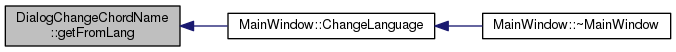
\includegraphics[width=350pt]{class_dialog_change_chord_name_ad7b50213d9f354cb647dbd096441da13_icgraph}
\end{center}
\end{figure}
\mbox{\label{class_dialog_change_chord_name_ab3c2099c5229fc6a39e40742b8eca1c0}} 
\index{Dialog\+Change\+Chord\+Name@{Dialog\+Change\+Chord\+Name}!get\+From\+Lang\+Index@{get\+From\+Lang\+Index}}
\index{get\+From\+Lang\+Index@{get\+From\+Lang\+Index}!Dialog\+Change\+Chord\+Name@{Dialog\+Change\+Chord\+Name}}
\subsubsection{get\+From\+Lang\+Index()}
{\footnotesize\ttfamily int Dialog\+Change\+Chord\+Name\+::get\+From\+Lang\+Index (\begin{DoxyParamCaption}{ }\end{DoxyParamCaption})}



get\+From\+Lang\+Index return index of From\+Lang combobox 

\begin{DoxyReturn}{Returns}
int with the value of index of From\+Lang 
\end{DoxyReturn}
\mbox{\label{class_dialog_change_chord_name_aabf4fd401905585a53a2adf0b33440f7}} 
\index{Dialog\+Change\+Chord\+Name@{Dialog\+Change\+Chord\+Name}!get\+From\+Min@{get\+From\+Min}}
\index{get\+From\+Min@{get\+From\+Min}!Dialog\+Change\+Chord\+Name@{Dialog\+Change\+Chord\+Name}}
\subsubsection{get\+From\+Min()}
{\footnotesize\ttfamily Q\+String Dialog\+Change\+Chord\+Name\+::get\+From\+Min (\begin{DoxyParamCaption}{ }\end{DoxyParamCaption})}



get\+From\+Min after change return Minor notation for from conversion. Exampele m or -\/ 

\begin{DoxyReturn}{Returns}
Q\+String with letter for minor 
\end{DoxyReturn}
Here is the caller graph for this function\+:\nopagebreak
\begin{figure}[H]
\begin{center}
\leavevmode
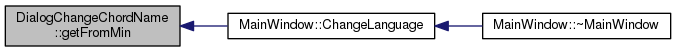
\includegraphics[width=350pt]{class_dialog_change_chord_name_aabf4fd401905585a53a2adf0b33440f7_icgraph}
\end{center}
\end{figure}
\mbox{\label{class_dialog_change_chord_name_a52880625729a9f1fd26387b1c6914027}} 
\index{Dialog\+Change\+Chord\+Name@{Dialog\+Change\+Chord\+Name}!get\+From\+Min\+Index@{get\+From\+Min\+Index}}
\index{get\+From\+Min\+Index@{get\+From\+Min\+Index}!Dialog\+Change\+Chord\+Name@{Dialog\+Change\+Chord\+Name}}
\subsubsection{get\+From\+Min\+Index()}
{\footnotesize\ttfamily int Dialog\+Change\+Chord\+Name\+::get\+From\+Min\+Index (\begin{DoxyParamCaption}{ }\end{DoxyParamCaption})}



get\+From\+Min\+Index return index of From\+Lang Combobox 

\begin{DoxyReturn}{Returns}
integer with the value of index of From\+Lang 
\end{DoxyReturn}
\mbox{\label{class_dialog_change_chord_name_a5626a4b248559874f30d04b71b11e11d}} 
\index{Dialog\+Change\+Chord\+Name@{Dialog\+Change\+Chord\+Name}!get\+To\+Lang@{get\+To\+Lang}}
\index{get\+To\+Lang@{get\+To\+Lang}!Dialog\+Change\+Chord\+Name@{Dialog\+Change\+Chord\+Name}}
\subsubsection{get\+To\+Lang()}
{\footnotesize\ttfamily Q\+String Dialog\+Change\+Chord\+Name\+::get\+To\+Lang (\begin{DoxyParamCaption}{ }\end{DoxyParamCaption})}



get\+To\+Lang after change return to language 

\begin{DoxyReturn}{Returns}
Q\+String for language for example Français or English 
\end{DoxyReturn}
Here is the caller graph for this function\+:\nopagebreak
\begin{figure}[H]
\begin{center}
\leavevmode
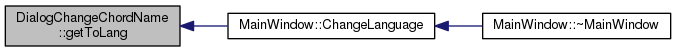
\includegraphics[width=350pt]{class_dialog_change_chord_name_a5626a4b248559874f30d04b71b11e11d_icgraph}
\end{center}
\end{figure}
\mbox{\label{class_dialog_change_chord_name_a2c7835cdfb841f3c9d375e44511ac5cc}} 
\index{Dialog\+Change\+Chord\+Name@{Dialog\+Change\+Chord\+Name}!get\+To\+Lang\+Index@{get\+To\+Lang\+Index}}
\index{get\+To\+Lang\+Index@{get\+To\+Lang\+Index}!Dialog\+Change\+Chord\+Name@{Dialog\+Change\+Chord\+Name}}
\subsubsection{get\+To\+Lang\+Index()}
{\footnotesize\ttfamily int Dialog\+Change\+Chord\+Name\+::get\+To\+Lang\+Index (\begin{DoxyParamCaption}{ }\end{DoxyParamCaption})}



get\+To\+Lang\+Index return index of To\+Lang Combobox 

\begin{DoxyReturn}{Returns}
integer with the value of index of From\+Lang 
\end{DoxyReturn}
Here is the caller graph for this function\+:\nopagebreak
\begin{figure}[H]
\begin{center}
\leavevmode
\includegraphics[width=350pt]{class_dialog_change_chord_name_a2c7835cdfb841f3c9d375e44511ac5cc_icgraph}
\end{center}
\end{figure}
\mbox{\label{class_dialog_change_chord_name_af7cd951023ca7af6a50cab16f06fdc00}} 
\index{Dialog\+Change\+Chord\+Name@{Dialog\+Change\+Chord\+Name}!get\+To\+Min@{get\+To\+Min}}
\index{get\+To\+Min@{get\+To\+Min}!Dialog\+Change\+Chord\+Name@{Dialog\+Change\+Chord\+Name}}
\subsubsection{get\+To\+Min()}
{\footnotesize\ttfamily Q\+String Dialog\+Change\+Chord\+Name\+::get\+To\+Min (\begin{DoxyParamCaption}{ }\end{DoxyParamCaption})}



get\+To\+Min after change return Minor notation for to conversion. Exampele m or -\/ 

\begin{DoxyReturn}{Returns}
Q\+String with letter for minor 
\end{DoxyReturn}
Here is the caller graph for this function\+:\nopagebreak
\begin{figure}[H]
\begin{center}
\leavevmode
\includegraphics[width=350pt]{class_dialog_change_chord_name_af7cd951023ca7af6a50cab16f06fdc00_icgraph}
\end{center}
\end{figure}
\mbox{\label{class_dialog_change_chord_name_aefc1211f4d9920f6d4e3124ec12c35d3}} 
\index{Dialog\+Change\+Chord\+Name@{Dialog\+Change\+Chord\+Name}!get\+To\+Min\+Index@{get\+To\+Min\+Index}}
\index{get\+To\+Min\+Index@{get\+To\+Min\+Index}!Dialog\+Change\+Chord\+Name@{Dialog\+Change\+Chord\+Name}}
\subsubsection{get\+To\+Min\+Index()}
{\footnotesize\ttfamily int Dialog\+Change\+Chord\+Name\+::get\+To\+Min\+Index (\begin{DoxyParamCaption}{ }\end{DoxyParamCaption})}



get\+To\+Min\+Index return index of To\+Lang Combobox 

\begin{DoxyReturn}{Returns}
integer with the value of index of To\+Lang 
\end{DoxyReturn}
Here is the caller graph for this function\+:\nopagebreak
\begin{figure}[H]
\begin{center}
\leavevmode
\includegraphics[width=350pt]{class_dialog_change_chord_name_aefc1211f4d9920f6d4e3124ec12c35d3_icgraph}
\end{center}
\end{figure}
\mbox{\label{class_dialog_change_chord_name_af61986ce1cd8973a004d5d75e3e5e50c}} 
\index{Dialog\+Change\+Chord\+Name@{Dialog\+Change\+Chord\+Name}!Ok\+Dialog@{Ok\+Dialog}}
\index{Ok\+Dialog@{Ok\+Dialog}!Dialog\+Change\+Chord\+Name@{Dialog\+Change\+Chord\+Name}}
\subsubsection{Ok\+Dialog()}
{\footnotesize\ttfamily bool Dialog\+Change\+Chord\+Name\+::\+Ok\+Dialog (\begin{DoxyParamCaption}{ }\end{DoxyParamCaption})}



Ok\+Dialog the dialog return ok (true) or cancel(false) 

\begin{DoxyReturn}{Returns}
the bool is true only if ok button is clicked 
\end{DoxyReturn}
Here is the caller graph for this function\+:\nopagebreak
\begin{figure}[H]
\begin{center}
\leavevmode
\includegraphics[width=350pt]{class_dialog_change_chord_name_af61986ce1cd8973a004d5d75e3e5e50c_icgraph}
\end{center}
\end{figure}
\mbox{\label{class_dialog_change_chord_name_a3b2ae74d078fe1f55f2eac9b762483da}} 
\index{Dialog\+Change\+Chord\+Name@{Dialog\+Change\+Chord\+Name}!set\+From\+Lang@{set\+From\+Lang}}
\index{set\+From\+Lang@{set\+From\+Lang}!Dialog\+Change\+Chord\+Name@{Dialog\+Change\+Chord\+Name}}
\subsubsection{set\+From\+Lang()}
{\footnotesize\ttfamily void Dialog\+Change\+Chord\+Name\+::set\+From\+Lang (\begin{DoxyParamCaption}\item[{int}]{lang }\end{DoxyParamCaption})}



set\+From\+Lang set the index of From\+Lang combobox 


\begin{DoxyParams}{Parameters}
{\em lang} & the index of From\+Lang \\
\hline
\end{DoxyParams}
Here is the caller graph for this function\+:\nopagebreak
\begin{figure}[H]
\begin{center}
\leavevmode
\includegraphics[width=350pt]{class_dialog_change_chord_name_a3b2ae74d078fe1f55f2eac9b762483da_icgraph}
\end{center}
\end{figure}
\mbox{\label{class_dialog_change_chord_name_a3f04e432b9099cdff2f07993f5d85811}} 
\index{Dialog\+Change\+Chord\+Name@{Dialog\+Change\+Chord\+Name}!set\+From\+Min@{set\+From\+Min}}
\index{set\+From\+Min@{set\+From\+Min}!Dialog\+Change\+Chord\+Name@{Dialog\+Change\+Chord\+Name}}
\subsubsection{set\+From\+Min()}
{\footnotesize\ttfamily void Dialog\+Change\+Chord\+Name\+::set\+From\+Min (\begin{DoxyParamCaption}\item[{int}]{lang }\end{DoxyParamCaption})}



set\+From\+Min idem with Minor letter 


\begin{DoxyParams}{Parameters}
{\em lang} & \\
\hline
\end{DoxyParams}
Here is the caller graph for this function\+:\nopagebreak
\begin{figure}[H]
\begin{center}
\leavevmode
\includegraphics[width=350pt]{class_dialog_change_chord_name_a3f04e432b9099cdff2f07993f5d85811_icgraph}
\end{center}
\end{figure}
\mbox{\label{class_dialog_change_chord_name_a90911cedcaff309a89161d18cca28227}} 
\index{Dialog\+Change\+Chord\+Name@{Dialog\+Change\+Chord\+Name}!set\+To\+Lang@{set\+To\+Lang}}
\index{set\+To\+Lang@{set\+To\+Lang}!Dialog\+Change\+Chord\+Name@{Dialog\+Change\+Chord\+Name}}
\subsubsection{set\+To\+Lang()}
{\footnotesize\ttfamily void Dialog\+Change\+Chord\+Name\+::set\+To\+Lang (\begin{DoxyParamCaption}\item[{int}]{min }\end{DoxyParamCaption})}



set\+To\+Lang set tje index of To\+From combobox 


\begin{DoxyParams}{Parameters}
{\em min} & the to langa \\
\hline
\end{DoxyParams}
Here is the caller graph for this function\+:\nopagebreak
\begin{figure}[H]
\begin{center}
\leavevmode
\includegraphics[width=350pt]{class_dialog_change_chord_name_a90911cedcaff309a89161d18cca28227_icgraph}
\end{center}
\end{figure}
\mbox{\label{class_dialog_change_chord_name_a5694384c88af005f6a8a949cfa43153c}} 
\index{Dialog\+Change\+Chord\+Name@{Dialog\+Change\+Chord\+Name}!set\+To\+Min@{set\+To\+Min}}
\index{set\+To\+Min@{set\+To\+Min}!Dialog\+Change\+Chord\+Name@{Dialog\+Change\+Chord\+Name}}
\subsubsection{set\+To\+Min()}
{\footnotesize\ttfamily void Dialog\+Change\+Chord\+Name\+::set\+To\+Min (\begin{DoxyParamCaption}\item[{int}]{min }\end{DoxyParamCaption})}



set\+To\+Min same as above with To record 


\begin{DoxyParams}{Parameters}
{\em min} & \\
\hline
\end{DoxyParams}
Here is the caller graph for this function\+:\nopagebreak
\begin{figure}[H]
\begin{center}
\leavevmode
\includegraphics[width=350pt]{class_dialog_change_chord_name_a5694384c88af005f6a8a949cfa43153c_icgraph}
\end{center}
\end{figure}


The documentation for this class was generated from the following files\+:\begin{DoxyCompactItemize}
\item 
src/\textbf{ dialogchangechordname.\+h}\item 
src/\textbf{ dialogchangechordname.\+cpp}\end{DoxyCompactItemize}

\section{Dialog\+Choose\+Good\+Chord Class Reference}
\label{class_dialog_choose_good_chord}\index{Dialog\+Choose\+Good\+Chord@{Dialog\+Choose\+Good\+Chord}}


{\ttfamily \#include $<$dialogchoosegoodchord.\+h$>$}



Inheritance diagram for Dialog\+Choose\+Good\+Chord\+:\nopagebreak
\begin{figure}[H]
\begin{center}
\leavevmode
\includegraphics[width=208pt]{class_dialog_choose_good_chord__inherit__graph}
\end{center}
\end{figure}


Collaboration diagram for Dialog\+Choose\+Good\+Chord\+:\nopagebreak
\begin{figure}[H]
\begin{center}
\leavevmode
\includegraphics[width=208pt]{class_dialog_choose_good_chord__coll__graph}
\end{center}
\end{figure}
\subsection*{Signals}
\begin{DoxyCompactItemize}
\item 
void \textbf{ Error} (Q\+String texterror)
\end{DoxyCompactItemize}
\subsection*{Public Member Functions}
\begin{DoxyCompactItemize}
\item 
\textbf{ Dialog\+Choose\+Good\+Chord} (Q\+String oldname, Q\+String oldvalue, Q\+String newname, Q\+String newvalue, Q\+Widget $\ast$parent=0)
\item 
\textbf{ $\sim$\+Dialog\+Choose\+Good\+Chord} ()
\end{DoxyCompactItemize}


\subsection{Constructor \& Destructor Documentation}
\mbox{\label{class_dialog_choose_good_chord_a42f1b2a7699d81ecacca7e60c9de8632}} 
\index{Dialog\+Choose\+Good\+Chord@{Dialog\+Choose\+Good\+Chord}!Dialog\+Choose\+Good\+Chord@{Dialog\+Choose\+Good\+Chord}}
\index{Dialog\+Choose\+Good\+Chord@{Dialog\+Choose\+Good\+Chord}!Dialog\+Choose\+Good\+Chord@{Dialog\+Choose\+Good\+Chord}}
\subsubsection{Dialog\+Choose\+Good\+Chord()}
{\footnotesize\ttfamily Dialog\+Choose\+Good\+Chord\+::\+Dialog\+Choose\+Good\+Chord (\begin{DoxyParamCaption}\item[{Q\+String}]{oldname,  }\item[{Q\+String}]{oldvalue,  }\item[{Q\+String}]{newname,  }\item[{Q\+String}]{newvalue,  }\item[{Q\+Widget $\ast$}]{parent = {\ttfamily 0} }\end{DoxyParamCaption})\hspace{0.3cm}{\ttfamily [explicit]}}

\mbox{\label{class_dialog_choose_good_chord_aa43c9d54cf25dfc64c477eca63ac79dd}} 
\index{Dialog\+Choose\+Good\+Chord@{Dialog\+Choose\+Good\+Chord}!````~Dialog\+Choose\+Good\+Chord@{$\sim$\+Dialog\+Choose\+Good\+Chord}}
\index{````~Dialog\+Choose\+Good\+Chord@{$\sim$\+Dialog\+Choose\+Good\+Chord}!Dialog\+Choose\+Good\+Chord@{Dialog\+Choose\+Good\+Chord}}
\subsubsection{$\sim$\+Dialog\+Choose\+Good\+Chord()}
{\footnotesize\ttfamily Dialog\+Choose\+Good\+Chord\+::$\sim$\+Dialog\+Choose\+Good\+Chord (\begin{DoxyParamCaption}{ }\end{DoxyParamCaption})}



\subsection{Member Function Documentation}
\mbox{\label{class_dialog_choose_good_chord_ae1efce45018b1515df4e7d136b7fbad7}} 
\index{Dialog\+Choose\+Good\+Chord@{Dialog\+Choose\+Good\+Chord}!Error@{Error}}
\index{Error@{Error}!Dialog\+Choose\+Good\+Chord@{Dialog\+Choose\+Good\+Chord}}
\subsubsection{Error}
{\footnotesize\ttfamily void Dialog\+Choose\+Good\+Chord\+::\+Error (\begin{DoxyParamCaption}\item[{Q\+String}]{texterror }\end{DoxyParamCaption})\hspace{0.3cm}{\ttfamily [signal]}}

Here is the caller graph for this function\+:\nopagebreak
\begin{figure}[H]
\begin{center}
\leavevmode
\includegraphics[width=350pt]{class_dialog_choose_good_chord_ae1efce45018b1515df4e7d136b7fbad7_icgraph}
\end{center}
\end{figure}


The documentation for this class was generated from the following files\+:\begin{DoxyCompactItemize}
\item 
src/\textbf{ dialogchoosegoodchord.\+h}\item 
src/\textbf{ dialogchoosegoodchord.\+cpp}\end{DoxyCompactItemize}

\section{Dialog\+Chord\+Definition Class Reference}
\label{class_dialog_chord_definition}\index{Dialog\+Chord\+Definition@{Dialog\+Chord\+Definition}}


{\ttfamily \#include $<$dialogchorddefinition.\+h$>$}



Inheritance diagram for Dialog\+Chord\+Definition\+:\nopagebreak
\begin{figure}[H]
\begin{center}
\leavevmode
\includegraphics[width=192pt]{class_dialog_chord_definition__inherit__graph}
\end{center}
\end{figure}


Collaboration diagram for Dialog\+Chord\+Definition\+:\nopagebreak
\begin{figure}[H]
\begin{center}
\leavevmode
\includegraphics[width=192pt]{class_dialog_chord_definition__coll__graph}
\end{center}
\end{figure}
\subsection*{Signals}
\begin{DoxyCompactItemize}
\item 
void \textbf{ Error} (Q\+String message)
\item 
void \textbf{ Chord\+To\+Insert} (Q\+String chord)
\end{DoxyCompactItemize}
\subsection*{Public Member Functions}
\begin{DoxyCompactItemize}
\item 
\textbf{ Dialog\+Chord\+Definition} (Q\+Widget $\ast$parent=0)
\item 
\textbf{ $\sim$\+Dialog\+Chord\+Definition} ()
\item 
void \textbf{ Set\+Chord\+Language} (Q\+String lang, Q\+String minor)
\item 
void \textbf{ Active\+Insert\+Button} ()
\end{DoxyCompactItemize}
\subsection*{Protected Slots}
\begin{DoxyCompactItemize}
\item 
void \textbf{ Show\+Chords} (Q\+String\+List chordnames, Q\+String chortdstring)
\end{DoxyCompactItemize}


\subsection{Constructor \& Destructor Documentation}
\mbox{\label{class_dialog_chord_definition_a01f03ae795540807e783a8a0e0afa9a2}} 
\index{Dialog\+Chord\+Definition@{Dialog\+Chord\+Definition}!Dialog\+Chord\+Definition@{Dialog\+Chord\+Definition}}
\index{Dialog\+Chord\+Definition@{Dialog\+Chord\+Definition}!Dialog\+Chord\+Definition@{Dialog\+Chord\+Definition}}
\subsubsection{Dialog\+Chord\+Definition()}
{\footnotesize\ttfamily Dialog\+Chord\+Definition\+::\+Dialog\+Chord\+Definition (\begin{DoxyParamCaption}\item[{Q\+Widget $\ast$}]{parent = {\ttfamily 0} }\end{DoxyParamCaption})\hspace{0.3cm}{\ttfamily [explicit]}}

Here is the call graph for this function\+:\nopagebreak
\begin{figure}[H]
\begin{center}
\leavevmode
\includegraphics[width=350pt]{class_dialog_chord_definition_a01f03ae795540807e783a8a0e0afa9a2_cgraph}
\end{center}
\end{figure}
\mbox{\label{class_dialog_chord_definition_a5a26fa1ceb8e4802e5c4d8d04db7b92f}} 
\index{Dialog\+Chord\+Definition@{Dialog\+Chord\+Definition}!````~Dialog\+Chord\+Definition@{$\sim$\+Dialog\+Chord\+Definition}}
\index{````~Dialog\+Chord\+Definition@{$\sim$\+Dialog\+Chord\+Definition}!Dialog\+Chord\+Definition@{Dialog\+Chord\+Definition}}
\subsubsection{$\sim$\+Dialog\+Chord\+Definition()}
{\footnotesize\ttfamily Dialog\+Chord\+Definition\+::$\sim$\+Dialog\+Chord\+Definition (\begin{DoxyParamCaption}{ }\end{DoxyParamCaption})}



\subsection{Member Function Documentation}
\mbox{\label{class_dialog_chord_definition_a0c0c9122565ddcac862ca32851a52963}} 
\index{Dialog\+Chord\+Definition@{Dialog\+Chord\+Definition}!Active\+Insert\+Button@{Active\+Insert\+Button}}
\index{Active\+Insert\+Button@{Active\+Insert\+Button}!Dialog\+Chord\+Definition@{Dialog\+Chord\+Definition}}
\subsubsection{Active\+Insert\+Button()}
{\footnotesize\ttfamily void Dialog\+Chord\+Definition\+::\+Active\+Insert\+Button (\begin{DoxyParamCaption}{ }\end{DoxyParamCaption})}

Here is the call graph for this function\+:\nopagebreak
\begin{figure}[H]
\begin{center}
\leavevmode
\includegraphics[width=350pt]{class_dialog_chord_definition_a0c0c9122565ddcac862ca32851a52963_cgraph}
\end{center}
\end{figure}
Here is the caller graph for this function\+:\nopagebreak
\begin{figure}[H]
\begin{center}
\leavevmode
\includegraphics[width=350pt]{class_dialog_chord_definition_a0c0c9122565ddcac862ca32851a52963_icgraph}
\end{center}
\end{figure}
\mbox{\label{class_dialog_chord_definition_ac543c959ed39cc4bc06b39f9841386cd}} 
\index{Dialog\+Chord\+Definition@{Dialog\+Chord\+Definition}!Chord\+To\+Insert@{Chord\+To\+Insert}}
\index{Chord\+To\+Insert@{Chord\+To\+Insert}!Dialog\+Chord\+Definition@{Dialog\+Chord\+Definition}}
\subsubsection{Chord\+To\+Insert}
{\footnotesize\ttfamily void Dialog\+Chord\+Definition\+::\+Chord\+To\+Insert (\begin{DoxyParamCaption}\item[{Q\+String}]{chord }\end{DoxyParamCaption})\hspace{0.3cm}{\ttfamily [signal]}}

Here is the caller graph for this function\+:\nopagebreak
\begin{figure}[H]
\begin{center}
\leavevmode
\includegraphics[width=350pt]{class_dialog_chord_definition_ac543c959ed39cc4bc06b39f9841386cd_icgraph}
\end{center}
\end{figure}
\mbox{\label{class_dialog_chord_definition_aac9b456634554d8bedf4c08c1531d8ea}} 
\index{Dialog\+Chord\+Definition@{Dialog\+Chord\+Definition}!Error@{Error}}
\index{Error@{Error}!Dialog\+Chord\+Definition@{Dialog\+Chord\+Definition}}
\subsubsection{Error}
{\footnotesize\ttfamily void Dialog\+Chord\+Definition\+::\+Error (\begin{DoxyParamCaption}\item[{Q\+String}]{message }\end{DoxyParamCaption})\hspace{0.3cm}{\ttfamily [signal]}}

Here is the caller graph for this function\+:\nopagebreak
\begin{figure}[H]
\begin{center}
\leavevmode
\includegraphics[width=350pt]{class_dialog_chord_definition_aac9b456634554d8bedf4c08c1531d8ea_icgraph}
\end{center}
\end{figure}
\mbox{\label{class_dialog_chord_definition_a068654bc3d37f448057fed1fd3058258}} 
\index{Dialog\+Chord\+Definition@{Dialog\+Chord\+Definition}!Set\+Chord\+Language@{Set\+Chord\+Language}}
\index{Set\+Chord\+Language@{Set\+Chord\+Language}!Dialog\+Chord\+Definition@{Dialog\+Chord\+Definition}}
\subsubsection{Set\+Chord\+Language()}
{\footnotesize\ttfamily void Dialog\+Chord\+Definition\+::\+Set\+Chord\+Language (\begin{DoxyParamCaption}\item[{Q\+String}]{lang,  }\item[{Q\+String}]{minor }\end{DoxyParamCaption})}

Here is the call graph for this function\+:\nopagebreak
\begin{figure}[H]
\begin{center}
\leavevmode
\includegraphics[width=350pt]{class_dialog_chord_definition_a068654bc3d37f448057fed1fd3058258_cgraph}
\end{center}
\end{figure}
Here is the caller graph for this function\+:\nopagebreak
\begin{figure}[H]
\begin{center}
\leavevmode
\includegraphics[width=350pt]{class_dialog_chord_definition_a068654bc3d37f448057fed1fd3058258_icgraph}
\end{center}
\end{figure}
\mbox{\label{class_dialog_chord_definition_af02305bf92afaf24d635e9a73f21d087}} 
\index{Dialog\+Chord\+Definition@{Dialog\+Chord\+Definition}!Show\+Chords@{Show\+Chords}}
\index{Show\+Chords@{Show\+Chords}!Dialog\+Chord\+Definition@{Dialog\+Chord\+Definition}}
\subsubsection{Show\+Chords}
{\footnotesize\ttfamily void Dialog\+Chord\+Definition\+::\+Show\+Chords (\begin{DoxyParamCaption}\item[{Q\+String\+List}]{chordnames,  }\item[{Q\+String}]{chortdstring }\end{DoxyParamCaption})\hspace{0.3cm}{\ttfamily [protected]}, {\ttfamily [slot]}}

Here is the call graph for this function\+:\nopagebreak
\begin{figure}[H]
\begin{center}
\leavevmode
\includegraphics[width=350pt]{class_dialog_chord_definition_af02305bf92afaf24d635e9a73f21d087_cgraph}
\end{center}
\end{figure}
Here is the caller graph for this function\+:\nopagebreak
\begin{figure}[H]
\begin{center}
\leavevmode
\includegraphics[width=346pt]{class_dialog_chord_definition_af02305bf92afaf24d635e9a73f21d087_icgraph}
\end{center}
\end{figure}


The documentation for this class was generated from the following files\+:\begin{DoxyCompactItemize}
\item 
src/\textbf{ dialogchorddefinition.\+h}\item 
src/\textbf{ dialogchorddefinition.\+cpp}\end{DoxyCompactItemize}

\section{Dialog\+Configuration Class Reference}
\label{class_dialog_configuration}\index{Dialog\+Configuration@{Dialog\+Configuration}}


{\ttfamily \#include $<$dialogconfiguration.\+h$>$}



Inheritance diagram for Dialog\+Configuration\+:\nopagebreak
\begin{figure}[H]
\begin{center}
\leavevmode
\includegraphics[width=182pt]{class_dialog_configuration__inherit__graph}
\end{center}
\end{figure}


Collaboration diagram for Dialog\+Configuration\+:\nopagebreak
\begin{figure}[H]
\begin{center}
\leavevmode
\includegraphics[width=182pt]{class_dialog_configuration__coll__graph}
\end{center}
\end{figure}
\subsection*{Signals}
\begin{DoxyCompactItemize}
\item 
void \textbf{ Language\+Changed} (Q\+String lang)
\item 
void \textbf{ Pdf\+Reader\+Changed} ()
\end{DoxyCompactItemize}
\subsection*{Public Member Functions}
\begin{DoxyCompactItemize}
\item 
\textbf{ Dialog\+Configuration} (Q\+Widget $\ast$parent=0)
\item 
void \textbf{ set\+Translator} (Q\+Translator $\ast$translator)
\item 
\textbf{ $\sim$\+Dialog\+Configuration} ()
\item 
void \textbf{ Init\+Settings} ()
\end{DoxyCompactItemize}
\subsection*{Static Public Member Functions}
\begin{DoxyCompactItemize}
\item 
static void \textbf{ set\+Language\+Combo\+Box} (Q\+Combo\+Box $\ast$ptr)
\item 
static Q\+String \textbf{ get\+Translation\+Qm\+File\+Name} (Q\+String lang)
\end{DoxyCompactItemize}


\subsection{Constructor \& Destructor Documentation}
\mbox{\label{class_dialog_configuration_a9cd827ec8ac95b73b88563a88c03dcda}} 
\index{Dialog\+Configuration@{Dialog\+Configuration}!Dialog\+Configuration@{Dialog\+Configuration}}
\index{Dialog\+Configuration@{Dialog\+Configuration}!Dialog\+Configuration@{Dialog\+Configuration}}
\subsubsection{Dialog\+Configuration()}
{\footnotesize\ttfamily Dialog\+Configuration\+::\+Dialog\+Configuration (\begin{DoxyParamCaption}\item[{Q\+Widget $\ast$}]{parent = {\ttfamily 0} }\end{DoxyParamCaption})\hspace{0.3cm}{\ttfamily [explicit]}}

Here is the call graph for this function\+:\nopagebreak
\begin{figure}[H]
\begin{center}
\leavevmode
\includegraphics[width=350pt]{class_dialog_configuration_a9cd827ec8ac95b73b88563a88c03dcda_cgraph}
\end{center}
\end{figure}
\mbox{\label{class_dialog_configuration_a3ee29dbe89f1f4653d4435c5914720d3}} 
\index{Dialog\+Configuration@{Dialog\+Configuration}!````~Dialog\+Configuration@{$\sim$\+Dialog\+Configuration}}
\index{````~Dialog\+Configuration@{$\sim$\+Dialog\+Configuration}!Dialog\+Configuration@{Dialog\+Configuration}}
\subsubsection{$\sim$\+Dialog\+Configuration()}
{\footnotesize\ttfamily Dialog\+Configuration\+::$\sim$\+Dialog\+Configuration (\begin{DoxyParamCaption}{ }\end{DoxyParamCaption})}

Here is the call graph for this function\+:\nopagebreak
\begin{figure}[H]
\begin{center}
\leavevmode
\includegraphics[width=350pt]{class_dialog_configuration_a3ee29dbe89f1f4653d4435c5914720d3_cgraph}
\end{center}
\end{figure}


\subsection{Member Function Documentation}
\mbox{\label{class_dialog_configuration_a9f8e92c1a10c3b510f2a841ce897e251}} 
\index{Dialog\+Configuration@{Dialog\+Configuration}!get\+Translation\+Qm\+File\+Name@{get\+Translation\+Qm\+File\+Name}}
\index{get\+Translation\+Qm\+File\+Name@{get\+Translation\+Qm\+File\+Name}!Dialog\+Configuration@{Dialog\+Configuration}}
\subsubsection{get\+Translation\+Qm\+File\+Name()}
{\footnotesize\ttfamily static Q\+String Dialog\+Configuration\+::get\+Translation\+Qm\+File\+Name (\begin{DoxyParamCaption}\item[{Q\+String}]{lang }\end{DoxyParamCaption})\hspace{0.3cm}{\ttfamily [static]}}

\mbox{\label{class_dialog_configuration_a89a10340bee6aaedae8111875e4d955f}} 
\index{Dialog\+Configuration@{Dialog\+Configuration}!Init\+Settings@{Init\+Settings}}
\index{Init\+Settings@{Init\+Settings}!Dialog\+Configuration@{Dialog\+Configuration}}
\subsubsection{Init\+Settings()}
{\footnotesize\ttfamily void Dialog\+Configuration\+::\+Init\+Settings (\begin{DoxyParamCaption}{ }\end{DoxyParamCaption})}

Here is the call graph for this function\+:\nopagebreak
\begin{figure}[H]
\begin{center}
\leavevmode
\includegraphics[width=300pt]{class_dialog_configuration_a89a10340bee6aaedae8111875e4d955f_cgraph}
\end{center}
\end{figure}
Here is the caller graph for this function\+:\nopagebreak
\begin{figure}[H]
\begin{center}
\leavevmode
\includegraphics[width=326pt]{class_dialog_configuration_a89a10340bee6aaedae8111875e4d955f_icgraph}
\end{center}
\end{figure}
\mbox{\label{class_dialog_configuration_a16c3d334fcc7169be13e364fa56b5d11}} 
\index{Dialog\+Configuration@{Dialog\+Configuration}!Language\+Changed@{Language\+Changed}}
\index{Language\+Changed@{Language\+Changed}!Dialog\+Configuration@{Dialog\+Configuration}}
\subsubsection{Language\+Changed}
{\footnotesize\ttfamily void Dialog\+Configuration\+::\+Language\+Changed (\begin{DoxyParamCaption}\item[{Q\+String}]{lang }\end{DoxyParamCaption})\hspace{0.3cm}{\ttfamily [signal]}}

Here is the caller graph for this function\+:\nopagebreak
\begin{figure}[H]
\begin{center}
\leavevmode
\includegraphics[width=334pt]{class_dialog_configuration_a16c3d334fcc7169be13e364fa56b5d11_icgraph}
\end{center}
\end{figure}
\mbox{\label{class_dialog_configuration_ad0fe0cfd13e3e1e5afb2a6bf96c4070e}} 
\index{Dialog\+Configuration@{Dialog\+Configuration}!Pdf\+Reader\+Changed@{Pdf\+Reader\+Changed}}
\index{Pdf\+Reader\+Changed@{Pdf\+Reader\+Changed}!Dialog\+Configuration@{Dialog\+Configuration}}
\subsubsection{Pdf\+Reader\+Changed}
{\footnotesize\ttfamily void Dialog\+Configuration\+::\+Pdf\+Reader\+Changed (\begin{DoxyParamCaption}{ }\end{DoxyParamCaption})\hspace{0.3cm}{\ttfamily [signal]}}

Here is the caller graph for this function\+:\nopagebreak
\begin{figure}[H]
\begin{center}
\leavevmode
\includegraphics[width=350pt]{class_dialog_configuration_ad0fe0cfd13e3e1e5afb2a6bf96c4070e_icgraph}
\end{center}
\end{figure}
\mbox{\label{class_dialog_configuration_a654c54543413073208c71774455ca1a8}} 
\index{Dialog\+Configuration@{Dialog\+Configuration}!set\+Language\+Combo\+Box@{set\+Language\+Combo\+Box}}
\index{set\+Language\+Combo\+Box@{set\+Language\+Combo\+Box}!Dialog\+Configuration@{Dialog\+Configuration}}
\subsubsection{set\+Language\+Combo\+Box()}
{\footnotesize\ttfamily static void Dialog\+Configuration\+::set\+Language\+Combo\+Box (\begin{DoxyParamCaption}\item[{Q\+Combo\+Box $\ast$}]{ptr }\end{DoxyParamCaption})\hspace{0.3cm}{\ttfamily [static]}}

\mbox{\label{class_dialog_configuration_a587bdb105b0113c8bf296acbd512d6a0}} 
\index{Dialog\+Configuration@{Dialog\+Configuration}!set\+Translator@{set\+Translator}}
\index{set\+Translator@{set\+Translator}!Dialog\+Configuration@{Dialog\+Configuration}}
\subsubsection{set\+Translator()}
{\footnotesize\ttfamily void Dialog\+Configuration\+::set\+Translator (\begin{DoxyParamCaption}\item[{Q\+Translator $\ast$}]{translator }\end{DoxyParamCaption})}

Here is the caller graph for this function\+:\nopagebreak
\begin{figure}[H]
\begin{center}
\leavevmode
\includegraphics[width=350pt]{class_dialog_configuration_a587bdb105b0113c8bf296acbd512d6a0_icgraph}
\end{center}
\end{figure}


The documentation for this class was generated from the following files\+:\begin{DoxyCompactItemize}
\item 
src/\textbf{ dialogconfiguration.\+h}\item 
src/\textbf{ dialogconfiguration.\+cpp}\end{DoxyCompactItemize}

\section{Dialog\+Documentation Class Reference}
\label{class_dialog_documentation}\index{Dialog\+Documentation@{Dialog\+Documentation}}


{\ttfamily \#include $<$dialogdocumentation.\+h$>$}



Inheritance diagram for Dialog\+Documentation\+:\nopagebreak
\begin{figure}[H]
\begin{center}
\leavevmode
\includegraphics[width=190pt]{class_dialog_documentation__inherit__graph}
\end{center}
\end{figure}


Collaboration diagram for Dialog\+Documentation\+:\nopagebreak
\begin{figure}[H]
\begin{center}
\leavevmode
\includegraphics[width=190pt]{class_dialog_documentation__coll__graph}
\end{center}
\end{figure}
\subsection*{Public Member Functions}
\begin{DoxyCompactItemize}
\item 
\textbf{ Dialog\+Documentation} (Q\+Widget $\ast$parent=0)
\item 
\textbf{ $\sim$\+Dialog\+Documentation} ()
\end{DoxyCompactItemize}


\subsection{Constructor \& Destructor Documentation}
\mbox{\label{class_dialog_documentation_ac499acb991012191d669730e00ce2707}} 
\index{Dialog\+Documentation@{Dialog\+Documentation}!Dialog\+Documentation@{Dialog\+Documentation}}
\index{Dialog\+Documentation@{Dialog\+Documentation}!Dialog\+Documentation@{Dialog\+Documentation}}
\subsubsection{Dialog\+Documentation()}
{\footnotesize\ttfamily Dialog\+Documentation\+::\+Dialog\+Documentation (\begin{DoxyParamCaption}\item[{Q\+Widget $\ast$}]{parent = {\ttfamily 0} }\end{DoxyParamCaption})\hspace{0.3cm}{\ttfamily [explicit]}}

Here is the call graph for this function\+:\nopagebreak
\begin{figure}[H]
\begin{center}
\leavevmode
\includegraphics[width=350pt]{class_dialog_documentation_ac499acb991012191d669730e00ce2707_cgraph}
\end{center}
\end{figure}
\mbox{\label{class_dialog_documentation_ae4fea41bbc228c960476a06dd9fb1b62}} 
\index{Dialog\+Documentation@{Dialog\+Documentation}!````~Dialog\+Documentation@{$\sim$\+Dialog\+Documentation}}
\index{````~Dialog\+Documentation@{$\sim$\+Dialog\+Documentation}!Dialog\+Documentation@{Dialog\+Documentation}}
\subsubsection{$\sim$\+Dialog\+Documentation()}
{\footnotesize\ttfamily Dialog\+Documentation\+::$\sim$\+Dialog\+Documentation (\begin{DoxyParamCaption}{ }\end{DoxyParamCaption})}



The documentation for this class was generated from the following files\+:\begin{DoxyCompactItemize}
\item 
src/\textbf{ dialogdocumentation.\+h}\item 
src/\textbf{ dialogdocumentation.\+cpp}\end{DoxyCompactItemize}

\section{Dialog\+New\+Song Class Reference}
\label{class_dialog_new_song}\index{Dialog\+New\+Song@{Dialog\+New\+Song}}


The \doxyref{Dialog\+New\+Song}{p.}{class_dialog_new_song} class this Dialog ask title, sybtitel, compress output yes or no, and column number for a song it provide a S\+I\+G\+N\+AL whe you clik on Insert button.  




{\ttfamily \#include $<$dialognewsong.\+h$>$}



Inheritance diagram for Dialog\+New\+Song\+:\nopagebreak
\begin{figure}[H]
\begin{center}
\leavevmode
\includegraphics[width=167pt]{class_dialog_new_song__inherit__graph}
\end{center}
\end{figure}


Collaboration diagram for Dialog\+New\+Song\+:\nopagebreak
\begin{figure}[H]
\begin{center}
\leavevmode
\includegraphics[width=167pt]{class_dialog_new_song__coll__graph}
\end{center}
\end{figure}
\subsection*{Signals}
\begin{DoxyCompactItemize}
\item 
void \textbf{ Insert\+Song} (Q\+String title, Q\+String subtitle, bool compress, int columns, int tempo, int time1, int time2)
\begin{DoxyCompactList}\small\item\em Insert\+Song signal sent when Insert button is clicked. \end{DoxyCompactList}\end{DoxyCompactItemize}
\subsection*{Public Member Functions}
\begin{DoxyCompactItemize}
\item 
\textbf{ Dialog\+New\+Song} (Q\+Widget $\ast$parent=0)
\begin{DoxyCompactList}\small\item\em \doxyref{Dialog\+New\+Song}{p.}{class_dialog_new_song} \+: classic constructor. \end{DoxyCompactList}\item 
\textbf{ $\sim$\+Dialog\+New\+Song} ()
\end{DoxyCompactItemize}


\subsection{Detailed Description}
The \doxyref{Dialog\+New\+Song}{p.}{class_dialog_new_song} class this Dialog ask title, sybtitel, compress output yes or no, and column number for a song it provide a S\+I\+G\+N\+AL whe you clik on Insert button. 

\subsection{Constructor \& Destructor Documentation}
\mbox{\label{class_dialog_new_song_a0b8f3bdb5a14b76d90fc2b652407c8eb}} 
\index{Dialog\+New\+Song@{Dialog\+New\+Song}!Dialog\+New\+Song@{Dialog\+New\+Song}}
\index{Dialog\+New\+Song@{Dialog\+New\+Song}!Dialog\+New\+Song@{Dialog\+New\+Song}}
\subsubsection{Dialog\+New\+Song()}
{\footnotesize\ttfamily Dialog\+New\+Song\+::\+Dialog\+New\+Song (\begin{DoxyParamCaption}\item[{Q\+Widget $\ast$}]{parent = {\ttfamily 0} }\end{DoxyParamCaption})\hspace{0.3cm}{\ttfamily [explicit]}}



\doxyref{Dialog\+New\+Song}{p.}{class_dialog_new_song} \+: classic constructor. 


\begin{DoxyParams}{Parameters}
{\em parent} & \+: parent window \\
\hline
\end{DoxyParams}
\mbox{\label{class_dialog_new_song_ae450c4fa2d4501cd4eb6be4093c593d1}} 
\index{Dialog\+New\+Song@{Dialog\+New\+Song}!````~Dialog\+New\+Song@{$\sim$\+Dialog\+New\+Song}}
\index{````~Dialog\+New\+Song@{$\sim$\+Dialog\+New\+Song}!Dialog\+New\+Song@{Dialog\+New\+Song}}
\subsubsection{$\sim$\+Dialog\+New\+Song()}
{\footnotesize\ttfamily Dialog\+New\+Song\+::$\sim$\+Dialog\+New\+Song (\begin{DoxyParamCaption}{ }\end{DoxyParamCaption})}



\subsection{Member Function Documentation}
\mbox{\label{class_dialog_new_song_ad932a09d06c3d5e8ca9a7d6965c6e7c5}} 
\index{Dialog\+New\+Song@{Dialog\+New\+Song}!Insert\+Song@{Insert\+Song}}
\index{Insert\+Song@{Insert\+Song}!Dialog\+New\+Song@{Dialog\+New\+Song}}
\subsubsection{Insert\+Song}
{\footnotesize\ttfamily void Dialog\+New\+Song\+::\+Insert\+Song (\begin{DoxyParamCaption}\item[{Q\+String}]{title,  }\item[{Q\+String}]{subtitle,  }\item[{bool}]{compress,  }\item[{int}]{columns,  }\item[{int}]{tempo,  }\item[{int}]{time1,  }\item[{int}]{time2 }\end{DoxyParamCaption})\hspace{0.3cm}{\ttfamily [signal]}}



Insert\+Song signal sent when Insert button is clicked. 


\begin{DoxyParams}{Parameters}
{\em title} & \+: title of song \\
\hline
{\em subtitle} & \+: subtitle \\
\hline
{\em compress} & \+: compress true or false \\
\hline
{\em columns} & \+: number of columns for the song \\
\hline
{\em tempo} & \+: the tempo or beat per minute default 120 \\
\hline
{\em time1} & \+: default 4 \+: 4 / 4 the second 4 is time2 \\
\hline
{\em time2} & \+: see time1 \\
\hline
\end{DoxyParams}
Here is the caller graph for this function\+:\nopagebreak
\begin{figure}[H]
\begin{center}
\leavevmode
\includegraphics[width=350pt]{class_dialog_new_song_ad932a09d06c3d5e8ca9a7d6965c6e7c5_icgraph}
\end{center}
\end{figure}


The documentation for this class was generated from the following files\+:\begin{DoxyCompactItemize}
\item 
src/\textbf{ dialognewsong.\+h}\item 
src/\textbf{ dialognewsong.\+cpp}\end{DoxyCompactItemize}

\section{Dialog\+Replace Class Reference}
\label{class_dialog_replace}\index{Dialog\+Replace@{Dialog\+Replace}}


The \doxyref{Dialog\+Replace}{p.}{class_dialog_replace} class allo to search and replace words in Editor.  




{\ttfamily \#include $<$dialogreplace.\+h$>$}



Inheritance diagram for Dialog\+Replace\+:\nopagebreak
\begin{figure}[H]
\begin{center}
\leavevmode
\includegraphics[width=160pt]{class_dialog_replace__inherit__graph}
\end{center}
\end{figure}


Collaboration diagram for Dialog\+Replace\+:\nopagebreak
\begin{figure}[H]
\begin{center}
\leavevmode
\includegraphics[width=160pt]{class_dialog_replace__coll__graph}
\end{center}
\end{figure}
\subsection*{Signals}
\begin{DoxyCompactItemize}
\item 
void \textbf{ Search\+Back} (Q\+String text, bool casesensitive, bool wordonly)
\item 
void \textbf{ Search} (Q\+String text, bool casesensitive, bool wordonly)
\item 
void \textbf{ Replace} (Q\+String textfrom, Q\+String textto, bool All, bool casesentisite, bool wordonly, bool back)
\end{DoxyCompactItemize}
\subsection*{Public Member Functions}
\begin{DoxyCompactItemize}
\item 
\textbf{ Dialog\+Replace} (Q\+Widget $\ast$parent=0)
\begin{DoxyCompactList}\small\item\em \doxyref{Dialog\+Replace}{p.}{class_dialog_replace} show a replace dialog to allow to search and replace inside Editor. \end{DoxyCompactList}\item 
\textbf{ $\sim$\+Dialog\+Replace} ()
\end{DoxyCompactItemize}


\subsection{Detailed Description}
The \doxyref{Dialog\+Replace}{p.}{class_dialog_replace} class allo to search and replace words in Editor. 

\subsection{Constructor \& Destructor Documentation}
\mbox{\label{class_dialog_replace_a8dad52d13d57e5d300894767396eb2b2}} 
\index{Dialog\+Replace@{Dialog\+Replace}!Dialog\+Replace@{Dialog\+Replace}}
\index{Dialog\+Replace@{Dialog\+Replace}!Dialog\+Replace@{Dialog\+Replace}}
\subsubsection{Dialog\+Replace()}
{\footnotesize\ttfamily Dialog\+Replace\+::\+Dialog\+Replace (\begin{DoxyParamCaption}\item[{Q\+Widget $\ast$}]{parent = {\ttfamily 0} }\end{DoxyParamCaption})\hspace{0.3cm}{\ttfamily [explicit]}}



\doxyref{Dialog\+Replace}{p.}{class_dialog_replace} show a replace dialog to allow to search and replace inside Editor. 


\begin{DoxyParams}{Parameters}
{\em parent} & \\
\hline
\end{DoxyParams}
\mbox{\label{class_dialog_replace_a520e8241ce741dcc190f2e199334190d}} 
\index{Dialog\+Replace@{Dialog\+Replace}!````~Dialog\+Replace@{$\sim$\+Dialog\+Replace}}
\index{````~Dialog\+Replace@{$\sim$\+Dialog\+Replace}!Dialog\+Replace@{Dialog\+Replace}}
\subsubsection{$\sim$\+Dialog\+Replace()}
{\footnotesize\ttfamily Dialog\+Replace\+::$\sim$\+Dialog\+Replace (\begin{DoxyParamCaption}{ }\end{DoxyParamCaption})}



\subsection{Member Function Documentation}
\mbox{\label{class_dialog_replace_ad67d3968f807518ac646c278ca5322e7}} 
\index{Dialog\+Replace@{Dialog\+Replace}!Replace@{Replace}}
\index{Replace@{Replace}!Dialog\+Replace@{Dialog\+Replace}}
\subsubsection{Replace}
{\footnotesize\ttfamily void Dialog\+Replace\+::\+Replace (\begin{DoxyParamCaption}\item[{Q\+String}]{textfrom,  }\item[{Q\+String}]{textto,  }\item[{bool}]{All,  }\item[{bool}]{casesentisite,  }\item[{bool}]{wordonly,  }\item[{bool}]{back }\end{DoxyParamCaption})\hspace{0.3cm}{\ttfamily [signal]}}

Here is the caller graph for this function\+:\nopagebreak
\begin{figure}[H]
\begin{center}
\leavevmode
\includegraphics[width=350pt]{class_dialog_replace_ad67d3968f807518ac646c278ca5322e7_icgraph}
\end{center}
\end{figure}
\mbox{\label{class_dialog_replace_a0c371007c3f5f5a3a7b70eef337f0a22}} 
\index{Dialog\+Replace@{Dialog\+Replace}!Search@{Search}}
\index{Search@{Search}!Dialog\+Replace@{Dialog\+Replace}}
\subsubsection{Search}
{\footnotesize\ttfamily void Dialog\+Replace\+::\+Search (\begin{DoxyParamCaption}\item[{Q\+String}]{text,  }\item[{bool}]{casesensitive,  }\item[{bool}]{wordonly }\end{DoxyParamCaption})\hspace{0.3cm}{\ttfamily [signal]}}

Here is the caller graph for this function\+:\nopagebreak
\begin{figure}[H]
\begin{center}
\leavevmode
\includegraphics[width=350pt]{class_dialog_replace_a0c371007c3f5f5a3a7b70eef337f0a22_icgraph}
\end{center}
\end{figure}
\mbox{\label{class_dialog_replace_ab4cae5f0d8b74c201857461e22781d5a}} 
\index{Dialog\+Replace@{Dialog\+Replace}!Search\+Back@{Search\+Back}}
\index{Search\+Back@{Search\+Back}!Dialog\+Replace@{Dialog\+Replace}}
\subsubsection{Search\+Back}
{\footnotesize\ttfamily void Dialog\+Replace\+::\+Search\+Back (\begin{DoxyParamCaption}\item[{Q\+String}]{text,  }\item[{bool}]{casesensitive,  }\item[{bool}]{wordonly }\end{DoxyParamCaption})\hspace{0.3cm}{\ttfamily [signal]}}

Here is the caller graph for this function\+:\nopagebreak
\begin{figure}[H]
\begin{center}
\leavevmode
\includegraphics[width=350pt]{class_dialog_replace_ab4cae5f0d8b74c201857461e22781d5a_icgraph}
\end{center}
\end{figure}


The documentation for this class was generated from the following files\+:\begin{DoxyCompactItemize}
\item 
src/\textbf{ dialogreplace.\+h}\item 
src/\textbf{ dialogreplace.\+cpp}\end{DoxyCompactItemize}

\section{Dialog\+Search Class Reference}
\label{class_dialog_search}\index{Dialog\+Search@{Dialog\+Search}}


The \doxyref{Dialog\+Search}{p.}{class_dialog_search} class allow to search word in Editor.  




{\ttfamily \#include $<$dialogsearch.\+h$>$}



Inheritance diagram for Dialog\+Search\+:\nopagebreak
\begin{figure}[H]
\begin{center}
\leavevmode
\includegraphics[width=155pt]{class_dialog_search__inherit__graph}
\end{center}
\end{figure}


Collaboration diagram for Dialog\+Search\+:\nopagebreak
\begin{figure}[H]
\begin{center}
\leavevmode
\includegraphics[width=155pt]{class_dialog_search__coll__graph}
\end{center}
\end{figure}
\subsection*{Signals}
\begin{DoxyCompactItemize}
\item 
void \textbf{ Search} (Q\+String text, bool casesensitive, bool wordonly)
\item 
void \textbf{ Search\+Back} (Q\+String text, bool casesensitive, bool wordonly)
\end{DoxyCompactItemize}
\subsection*{Public Member Functions}
\begin{DoxyCompactItemize}
\item 
\textbf{ Dialog\+Search} (Q\+Widget $\ast$parent=0)
\begin{DoxyCompactList}\small\item\em \doxyref{Dialog\+Search}{p.}{class_dialog_search} when the \doxyref{Dialog\+Search}{p.}{class_dialog_search} dialog is shown, user can choose word to search and relative features. \end{DoxyCompactList}\item 
\textbf{ $\sim$\+Dialog\+Search} ()
\end{DoxyCompactItemize}


\subsection{Detailed Description}
The \doxyref{Dialog\+Search}{p.}{class_dialog_search} class allow to search word in Editor. 

\subsection{Constructor \& Destructor Documentation}
\mbox{\label{class_dialog_search_a995391af8edd0494be2d399f5dc63fb4}} 
\index{Dialog\+Search@{Dialog\+Search}!Dialog\+Search@{Dialog\+Search}}
\index{Dialog\+Search@{Dialog\+Search}!Dialog\+Search@{Dialog\+Search}}
\subsubsection{Dialog\+Search()}
{\footnotesize\ttfamily Dialog\+Search\+::\+Dialog\+Search (\begin{DoxyParamCaption}\item[{Q\+Widget $\ast$}]{parent = {\ttfamily 0} }\end{DoxyParamCaption})\hspace{0.3cm}{\ttfamily [explicit]}}



\doxyref{Dialog\+Search}{p.}{class_dialog_search} when the \doxyref{Dialog\+Search}{p.}{class_dialog_search} dialog is shown, user can choose word to search and relative features. 


\begin{DoxyParams}{Parameters}
{\em parent} & \+: the parent Widget \\
\hline
\end{DoxyParams}
\mbox{\label{class_dialog_search_ac0cb32eda3c080ba88a49d3543803a73}} 
\index{Dialog\+Search@{Dialog\+Search}!````~Dialog\+Search@{$\sim$\+Dialog\+Search}}
\index{````~Dialog\+Search@{$\sim$\+Dialog\+Search}!Dialog\+Search@{Dialog\+Search}}
\subsubsection{$\sim$\+Dialog\+Search()}
{\footnotesize\ttfamily Dialog\+Search\+::$\sim$\+Dialog\+Search (\begin{DoxyParamCaption}{ }\end{DoxyParamCaption})}



\subsection{Member Function Documentation}
\mbox{\label{class_dialog_search_a1094b5ecb54df00abd56f18f80ae5b97}} 
\index{Dialog\+Search@{Dialog\+Search}!Search@{Search}}
\index{Search@{Search}!Dialog\+Search@{Dialog\+Search}}
\subsubsection{Search}
{\footnotesize\ttfamily void Dialog\+Search\+::\+Search (\begin{DoxyParamCaption}\item[{Q\+String}]{text,  }\item[{bool}]{casesensitive,  }\item[{bool}]{wordonly }\end{DoxyParamCaption})\hspace{0.3cm}{\ttfamily [signal]}}

\mbox{\label{class_dialog_search_ac6722d2b199a605a01857aafce79ee1f}} 
\index{Dialog\+Search@{Dialog\+Search}!Search\+Back@{Search\+Back}}
\index{Search\+Back@{Search\+Back}!Dialog\+Search@{Dialog\+Search}}
\subsubsection{Search\+Back}
{\footnotesize\ttfamily void Dialog\+Search\+::\+Search\+Back (\begin{DoxyParamCaption}\item[{Q\+String}]{text,  }\item[{bool}]{casesensitive,  }\item[{bool}]{wordonly }\end{DoxyParamCaption})\hspace{0.3cm}{\ttfamily [signal]}}

Here is the caller graph for this function\+:\nopagebreak
\begin{figure}[H]
\begin{center}
\leavevmode
\includegraphics[width=350pt]{class_dialog_search_ac6722d2b199a605a01857aafce79ee1f_icgraph}
\end{center}
\end{figure}


The documentation for this class was generated from the following files\+:\begin{DoxyCompactItemize}
\item 
src/\textbf{ dialogsearch.\+h}\item 
src/\textbf{ dialogsearch.\+cpp}\end{DoxyCompactItemize}

\section{Dialog\+System\+Info Class Reference}
\label{class_dialog_system_info}\index{Dialog\+System\+Info@{Dialog\+System\+Info}}


The \doxyref{Dialog\+System\+Info}{p.}{class_dialog_system_info} class this dialog show a set of system informations like date of compilation, release version, Git S\+H\+A1 version, program arguments, configuration file, Database location, P\+ID of process, location of language information.  




{\ttfamily \#include $<$dialogsysteminfo.\+h$>$}



Inheritance diagram for Dialog\+System\+Info\+:\nopagebreak
\begin{figure}[H]
\begin{center}
\leavevmode
\includegraphics[width=175pt]{class_dialog_system_info__inherit__graph}
\end{center}
\end{figure}


Collaboration diagram for Dialog\+System\+Info\+:\nopagebreak
\begin{figure}[H]
\begin{center}
\leavevmode
\includegraphics[width=175pt]{class_dialog_system_info__coll__graph}
\end{center}
\end{figure}
\subsection*{Public Member Functions}
\begin{DoxyCompactItemize}
\item 
\textbf{ Dialog\+System\+Info} (Q\+Widget $\ast$parent=0)
\begin{DoxyCompactList}\small\item\em \doxyref{Dialog\+System\+Info}{p.}{class_dialog_system_info} the constructor open the dialog window with parent giver in argument. \end{DoxyCompactList}\item 
\textbf{ $\sim$\+Dialog\+System\+Info} ()
\end{DoxyCompactItemize}


\subsection{Detailed Description}
The \doxyref{Dialog\+System\+Info}{p.}{class_dialog_system_info} class this dialog show a set of system informations like date of compilation, release version, Git S\+H\+A1 version, program arguments, configuration file, Database location, P\+ID of process, location of language information. 

\subsection{Constructor \& Destructor Documentation}
\mbox{\label{class_dialog_system_info_a9e6156904748af17840ee55c8233593e}} 
\index{Dialog\+System\+Info@{Dialog\+System\+Info}!Dialog\+System\+Info@{Dialog\+System\+Info}}
\index{Dialog\+System\+Info@{Dialog\+System\+Info}!Dialog\+System\+Info@{Dialog\+System\+Info}}
\subsubsection{Dialog\+System\+Info()}
{\footnotesize\ttfamily Dialog\+System\+Info\+::\+Dialog\+System\+Info (\begin{DoxyParamCaption}\item[{Q\+Widget $\ast$}]{parent = {\ttfamily 0} }\end{DoxyParamCaption})\hspace{0.3cm}{\ttfamily [explicit]}}



\doxyref{Dialog\+System\+Info}{p.}{class_dialog_system_info} the constructor open the dialog window with parent giver in argument. 


\begin{DoxyParams}{Parameters}
{\em parent} & \\
\hline
\end{DoxyParams}
\mbox{\label{class_dialog_system_info_a028fcd02f2d53a5e15e8eb2611bf4dcc}} 
\index{Dialog\+System\+Info@{Dialog\+System\+Info}!````~Dialog\+System\+Info@{$\sim$\+Dialog\+System\+Info}}
\index{````~Dialog\+System\+Info@{$\sim$\+Dialog\+System\+Info}!Dialog\+System\+Info@{Dialog\+System\+Info}}
\subsubsection{$\sim$\+Dialog\+System\+Info()}
{\footnotesize\ttfamily Dialog\+System\+Info\+::$\sim$\+Dialog\+System\+Info (\begin{DoxyParamCaption}{ }\end{DoxyParamCaption})}



The documentation for this class was generated from the following files\+:\begin{DoxyCompactItemize}
\item 
src/\textbf{ dialogsysteminfo.\+h}\item 
src/\textbf{ dialogsysteminfo.\+cpp}\end{DoxyCompactItemize}

\section{Dialog\+Transpose Class Reference}
\label{class_dialog_transpose}\index{Dialog\+Transpose@{Dialog\+Transpose}}


The \doxyref{Dialog\+Transpose}{p.}{class_dialog_transpose} class is a Dialog class to ask how many chroma negative or positive the user wants to transpose. It ask if the chord has to be with parenthesis or no and ask if just the current chord has to print translated, all the chord in the current line, all the chord on the current song or all the chord of the current booklet.  




{\ttfamily \#include $<$dialogtranspose.\+h$>$}



Inheritance diagram for Dialog\+Transpose\+:\nopagebreak
\begin{figure}[H]
\begin{center}
\leavevmode
\includegraphics[width=170pt]{class_dialog_transpose__inherit__graph}
\end{center}
\end{figure}


Collaboration diagram for Dialog\+Transpose\+:\nopagebreak
\begin{figure}[H]
\begin{center}
\leavevmode
\includegraphics[width=170pt]{class_dialog_transpose__coll__graph}
\end{center}
\end{figure}
\subsection*{Signals}
\begin{DoxyCompactItemize}
\item 
void \textbf{ Ask\+Change} (int halftonenumber, bool parenthesis, int Range)
\begin{DoxyCompactList}\small\item\em Ask\+Change ask change with halftonenumber, parenthesis yes or no, and range defined as just the current chord has to print translated, all the chord in the current line, all the chord on the current song or all the chord of the current booklet. \end{DoxyCompactList}\end{DoxyCompactItemize}
\subsection*{Public Member Functions}
\begin{DoxyCompactItemize}
\item 
\textbf{ Dialog\+Transpose} (Q\+Widget $\ast$parent=0)
\begin{DoxyCompactList}\small\item\em \doxyref{Dialog\+Transpose}{p.}{class_dialog_transpose} the Q\+Dialog constructor. \end{DoxyCompactList}\item 
\textbf{ $\sim$\+Dialog\+Transpose} ()
\end{DoxyCompactItemize}


\subsection{Detailed Description}
The \doxyref{Dialog\+Transpose}{p.}{class_dialog_transpose} class is a Dialog class to ask how many chroma negative or positive the user wants to transpose. It ask if the chord has to be with parenthesis or no and ask if just the current chord has to print translated, all the chord in the current line, all the chord on the current song or all the chord of the current booklet. 

\subsection{Constructor \& Destructor Documentation}
\mbox{\label{class_dialog_transpose_a55f63305272d5a2beff1592af45fdb23}} 
\index{Dialog\+Transpose@{Dialog\+Transpose}!Dialog\+Transpose@{Dialog\+Transpose}}
\index{Dialog\+Transpose@{Dialog\+Transpose}!Dialog\+Transpose@{Dialog\+Transpose}}
\subsubsection{Dialog\+Transpose()}
{\footnotesize\ttfamily Dialog\+Transpose\+::\+Dialog\+Transpose (\begin{DoxyParamCaption}\item[{Q\+Widget $\ast$}]{parent = {\ttfamily 0} }\end{DoxyParamCaption})\hspace{0.3cm}{\ttfamily [explicit]}}



\doxyref{Dialog\+Transpose}{p.}{class_dialog_transpose} the Q\+Dialog constructor. 


\begin{DoxyParams}{Parameters}
{\em parent} & \\
\hline
\end{DoxyParams}
\mbox{\label{class_dialog_transpose_ac4c34a3b948c25dca64197caed56938a}} 
\index{Dialog\+Transpose@{Dialog\+Transpose}!````~Dialog\+Transpose@{$\sim$\+Dialog\+Transpose}}
\index{````~Dialog\+Transpose@{$\sim$\+Dialog\+Transpose}!Dialog\+Transpose@{Dialog\+Transpose}}
\subsubsection{$\sim$\+Dialog\+Transpose()}
{\footnotesize\ttfamily Dialog\+Transpose\+::$\sim$\+Dialog\+Transpose (\begin{DoxyParamCaption}{ }\end{DoxyParamCaption})}



\subsection{Member Function Documentation}
\mbox{\label{class_dialog_transpose_aa4274bc33b9a92b0f9dff72c6b7d3e3b}} 
\index{Dialog\+Transpose@{Dialog\+Transpose}!Ask\+Change@{Ask\+Change}}
\index{Ask\+Change@{Ask\+Change}!Dialog\+Transpose@{Dialog\+Transpose}}
\subsubsection{Ask\+Change}
{\footnotesize\ttfamily void Dialog\+Transpose\+::\+Ask\+Change (\begin{DoxyParamCaption}\item[{int}]{halftonenumber,  }\item[{bool}]{parenthesis,  }\item[{int}]{Range }\end{DoxyParamCaption})\hspace{0.3cm}{\ttfamily [signal]}}



Ask\+Change ask change with halftonenumber, parenthesis yes or no, and range defined as just the current chord has to print translated, all the chord in the current line, all the chord on the current song or all the chord of the current booklet. 


\begin{DoxyParams}{Parameters}
{\em halftonenumber} & \\
\hline
{\em parenthesis} & \\
\hline
{\em Range} & \\
\hline
\end{DoxyParams}
Here is the caller graph for this function\+:
\nopagebreak
\begin{figure}[H]
\begin{center}
\leavevmode
\includegraphics[width=350pt]{class_dialog_transpose_aa4274bc33b9a92b0f9dff72c6b7d3e3b_icgraph}
\end{center}
\end{figure}


The documentation for this class was generated from the following files\+:\begin{DoxyCompactItemize}
\item 
src/\textbf{ dialogtranspose.\+h}\item 
src/\textbf{ dialogtranspose.\+cpp}\end{DoxyCompactItemize}

\section{Dialog\+Two\+Lines\+To\+Chord\+Pro Class Reference}
\label{class_dialog_two_lines_to_chord_pro}\index{Dialog\+Two\+Lines\+To\+Chord\+Pro@{Dialog\+Two\+Lines\+To\+Chord\+Pro}}


The \doxyref{Dialog\+Two\+Lines\+To\+Chord\+Pro}{p.}{class_dialog_two_lines_to_chord_pro} class is an utility to convert song in two lines \+:  




{\ttfamily \#include $<$dialogtwolinestochordpro.\+h$>$}



Inheritance diagram for Dialog\+Two\+Lines\+To\+Chord\+Pro\+:\nopagebreak
\begin{figure}[H]
\begin{center}
\leavevmode
\includegraphics[width=219pt]{class_dialog_two_lines_to_chord_pro__inherit__graph}
\end{center}
\end{figure}


Collaboration diagram for Dialog\+Two\+Lines\+To\+Chord\+Pro\+:\nopagebreak
\begin{figure}[H]
\begin{center}
\leavevmode
\includegraphics[width=219pt]{class_dialog_two_lines_to_chord_pro__coll__graph}
\end{center}
\end{figure}
\subsection*{Public Member Functions}
\begin{DoxyCompactItemize}
\item 
\textbf{ Dialog\+Two\+Lines\+To\+Chord\+Pro} (Q\+Widget $\ast$parent=0)
\begin{DoxyCompactList}\small\item\em \doxyref{Dialog\+Two\+Lines\+To\+Chord\+Pro}{p.}{class_dialog_two_lines_to_chord_pro} the dialog windows. \end{DoxyCompactList}\item 
\textbf{ $\sim$\+Dialog\+Two\+Lines\+To\+Chord\+Pro} ()
\end{DoxyCompactItemize}


\subsection{Detailed Description}
The \doxyref{Dialog\+Two\+Lines\+To\+Chord\+Pro}{p.}{class_dialog_two_lines_to_chord_pro} class is an utility to convert song in two lines \+: 

C D Hello how are you

to chord in one line \+: [C] Hello how are [D]you 

\subsection{Constructor \& Destructor Documentation}
\mbox{\label{class_dialog_two_lines_to_chord_pro_a3f1a4db647b4cca0043e4df52f6a4150}} 
\index{Dialog\+Two\+Lines\+To\+Chord\+Pro@{Dialog\+Two\+Lines\+To\+Chord\+Pro}!Dialog\+Two\+Lines\+To\+Chord\+Pro@{Dialog\+Two\+Lines\+To\+Chord\+Pro}}
\index{Dialog\+Two\+Lines\+To\+Chord\+Pro@{Dialog\+Two\+Lines\+To\+Chord\+Pro}!Dialog\+Two\+Lines\+To\+Chord\+Pro@{Dialog\+Two\+Lines\+To\+Chord\+Pro}}
\subsubsection{Dialog\+Two\+Lines\+To\+Chord\+Pro()}
{\footnotesize\ttfamily Dialog\+Two\+Lines\+To\+Chord\+Pro\+::\+Dialog\+Two\+Lines\+To\+Chord\+Pro (\begin{DoxyParamCaption}\item[{Q\+Widget $\ast$}]{parent = {\ttfamily 0} }\end{DoxyParamCaption})\hspace{0.3cm}{\ttfamily [explicit]}}



\doxyref{Dialog\+Two\+Lines\+To\+Chord\+Pro}{p.}{class_dialog_two_lines_to_chord_pro} the dialog windows. 


\begin{DoxyParams}{Parameters}
{\em parent} & \\
\hline
\end{DoxyParams}
\mbox{\label{class_dialog_two_lines_to_chord_pro_a37d4d5bd2e7d86589fa4bd9b3f96661c}} 
\index{Dialog\+Two\+Lines\+To\+Chord\+Pro@{Dialog\+Two\+Lines\+To\+Chord\+Pro}!````~Dialog\+Two\+Lines\+To\+Chord\+Pro@{$\sim$\+Dialog\+Two\+Lines\+To\+Chord\+Pro}}
\index{````~Dialog\+Two\+Lines\+To\+Chord\+Pro@{$\sim$\+Dialog\+Two\+Lines\+To\+Chord\+Pro}!Dialog\+Two\+Lines\+To\+Chord\+Pro@{Dialog\+Two\+Lines\+To\+Chord\+Pro}}
\subsubsection{$\sim$\+Dialog\+Two\+Lines\+To\+Chord\+Pro()}
{\footnotesize\ttfamily Dialog\+Two\+Lines\+To\+Chord\+Pro\+::$\sim$\+Dialog\+Two\+Lines\+To\+Chord\+Pro (\begin{DoxyParamCaption}{ }\end{DoxyParamCaption})}

Here is the call graph for this function\+:\nopagebreak
\begin{figure}[H]
\begin{center}
\leavevmode
\includegraphics[width=350pt]{class_dialog_two_lines_to_chord_pro_a37d4d5bd2e7d86589fa4bd9b3f96661c_cgraph}
\end{center}
\end{figure}


The documentation for this class was generated from the following files\+:\begin{DoxyCompactItemize}
\item 
src/\textbf{ dialogtwolinestochordpro.\+h}\item 
src/\textbf{ dialogtwolinestochordpro.\+cpp}\end{DoxyCompactItemize}

\section{Editor\+Highlighter Class Reference}
\label{class_editor_highlighter}\index{Editor\+Highlighter@{Editor\+Highlighter}}


{\ttfamily \#include $<$editorhighlighter.\+h$>$}



Inheritance diagram for Editor\+Highlighter\+:\nopagebreak
\begin{figure}[H]
\begin{center}
\leavevmode
\includegraphics[width=181pt]{class_editor_highlighter__inherit__graph}
\end{center}
\end{figure}


Collaboration diagram for Editor\+Highlighter\+:\nopagebreak
\begin{figure}[H]
\begin{center}
\leavevmode
\includegraphics[width=181pt]{class_editor_highlighter__coll__graph}
\end{center}
\end{figure}
\subsection*{Public Member Functions}
\begin{DoxyCompactItemize}
\item 
\textbf{ Editor\+Highlighter} (Q\+Text\+Document $\ast$parent)
\item 
void \textbf{ highlight\+Block} (const Q\+String \&text)
\end{DoxyCompactItemize}


\subsection{Constructor \& Destructor Documentation}
\mbox{\label{class_editor_highlighter_a73aaa3ba7c9c56cbf84f9446f3419ba5}} 
\index{Editor\+Highlighter@{Editor\+Highlighter}!Editor\+Highlighter@{Editor\+Highlighter}}
\index{Editor\+Highlighter@{Editor\+Highlighter}!Editor\+Highlighter@{Editor\+Highlighter}}
\subsubsection{Editor\+Highlighter()}
{\footnotesize\ttfamily Editor\+Highlighter\+::\+Editor\+Highlighter (\begin{DoxyParamCaption}\item[{Q\+Text\+Document $\ast$}]{parent }\end{DoxyParamCaption})}



\subsection{Member Function Documentation}
\mbox{\label{class_editor_highlighter_a78b64f41ec396f40a6f48e9f939f809e}} 
\index{Editor\+Highlighter@{Editor\+Highlighter}!highlight\+Block@{highlight\+Block}}
\index{highlight\+Block@{highlight\+Block}!Editor\+Highlighter@{Editor\+Highlighter}}
\subsubsection{highlight\+Block()}
{\footnotesize\ttfamily void Editor\+Highlighter\+::highlight\+Block (\begin{DoxyParamCaption}\item[{const Q\+String \&}]{text }\end{DoxyParamCaption})}



The documentation for this class was generated from the following files\+:\begin{DoxyCompactItemize}
\item 
src/\textbf{ editorhighlighter.\+h}\item 
src/\textbf{ editorhighlighter.\+cpp}\end{DoxyCompactItemize}

\section{Example\+Label Class Reference}
\label{class_example_label}\index{Example\+Label@{Example\+Label}}


{\ttfamily \#include $<$examplelabel.\+h$>$}



Inheritance diagram for Example\+Label\+:\nopagebreak
\begin{figure}[H]
\begin{center}
\leavevmode
\includegraphics[width=158pt]{class_example_label__inherit__graph}
\end{center}
\end{figure}


Collaboration diagram for Example\+Label\+:\nopagebreak
\begin{figure}[H]
\begin{center}
\leavevmode
\includegraphics[width=158pt]{class_example_label__coll__graph}
\end{center}
\end{figure}
\subsection*{Public Member Functions}
\begin{DoxyCompactItemize}
\item 
\textbf{ Example\+Label} (Q\+Widget $\ast$parent=0, Qt\+::\+Window\+Flags f=0)
\item 
void \textbf{ set\+Color} (Q\+Font font, Q\+Color color, Q\+Color background)
\end{DoxyCompactItemize}


\subsection{Constructor \& Destructor Documentation}
\mbox{\label{class_example_label_ab2dd91990a25cd0581460daaa9a8cf20}} 
\index{Example\+Label@{Example\+Label}!Example\+Label@{Example\+Label}}
\index{Example\+Label@{Example\+Label}!Example\+Label@{Example\+Label}}
\subsubsection{Example\+Label()}
{\footnotesize\ttfamily Example\+Label\+::\+Example\+Label (\begin{DoxyParamCaption}\item[{Q\+Widget $\ast$}]{parent = {\ttfamily 0},  }\item[{Qt\+::\+Window\+Flags}]{f = {\ttfamily 0} }\end{DoxyParamCaption})}



\subsection{Member Function Documentation}
\mbox{\label{class_example_label_a66dd209c3cc1d295c20b4d7c0450e60b}} 
\index{Example\+Label@{Example\+Label}!set\+Color@{set\+Color}}
\index{set\+Color@{set\+Color}!Example\+Label@{Example\+Label}}
\subsubsection{set\+Color()}
{\footnotesize\ttfamily void Example\+Label\+::set\+Color (\begin{DoxyParamCaption}\item[{Q\+Font}]{font,  }\item[{Q\+Color}]{color,  }\item[{Q\+Color}]{background }\end{DoxyParamCaption})}

Here is the caller graph for this function\+:\nopagebreak
\begin{figure}[H]
\begin{center}
\leavevmode
\includegraphics[width=333pt]{class_example_label_a66dd209c3cc1d295c20b4d7c0450e60b_icgraph}
\end{center}
\end{figure}


The documentation for this class was generated from the following files\+:\begin{DoxyCompactItemize}
\item 
src/\textbf{ examplelabel.\+h}\item 
src/\textbf{ examplelabel.\+cpp}\end{DoxyCompactItemize}

\section{Font\+Button Class Reference}
\label{class_font_button}\index{Font\+Button@{Font\+Button}}


{\ttfamily \#include $<$fontbutton.\+h$>$}



Inheritance diagram for Font\+Button\+:\nopagebreak
\begin{figure}[H]
\begin{center}
\leavevmode
\includegraphics[width=151pt]{class_font_button__inherit__graph}
\end{center}
\end{figure}


Collaboration diagram for Font\+Button\+:\nopagebreak
\begin{figure}[H]
\begin{center}
\leavevmode
\includegraphics[width=151pt]{class_font_button__coll__graph}
\end{center}
\end{figure}
\subsection*{Public Slots}
\begin{DoxyCompactItemize}
\item 
void \textbf{ Selected\+Font} (Q\+Font font, Q\+Color text, Q\+Color background)
\end{DoxyCompactItemize}
\subsection*{Signals}
\begin{DoxyCompactItemize}
\item 
void \textbf{ send\+Selected\+Font} (Q\+Font font, Q\+Color text, Q\+Color background)
\end{DoxyCompactItemize}
\subsection*{Public Member Functions}
\begin{DoxyCompactItemize}
\item 
\textbf{ Font\+Button} (Q\+Widget $\ast$parent)
\item 
void \textbf{ set\+Family} (Q\+String family)
\item 
void \textbf{ set\+Color} (Q\+Color color)
\item 
void \textbf{ set\+Background\+Color} (Q\+Color color)
\item 
void \textbf{ set\+Weight} (int i)
\item 
void \textbf{ set\+Italic} (bool b)
\item 
void \textbf{ set\+Pointsize} (int size)
\item 
void \textbf{ set\+Font} (Q\+Font font)
\item 
Q\+Font \textbf{ get\+Font} ()
\item 
Q\+Color \textbf{ get\+Background\+Color} ()
\item 
Q\+Color \textbf{ get\+Text\+Color} ()
\end{DoxyCompactItemize}


\subsection{Constructor \& Destructor Documentation}
\mbox{\label{class_font_button_a674ba43dfae18d276d2c0da64c5f9e24}} 
\index{Font\+Button@{Font\+Button}!Font\+Button@{Font\+Button}}
\index{Font\+Button@{Font\+Button}!Font\+Button@{Font\+Button}}
\subsubsection{Font\+Button()}
{\footnotesize\ttfamily Font\+Button\+::\+Font\+Button (\begin{DoxyParamCaption}\item[{Q\+Widget $\ast$}]{parent }\end{DoxyParamCaption})}

Here is the call graph for this function\+:\nopagebreak
\begin{figure}[H]
\begin{center}
\leavevmode
\includegraphics[width=350pt]{class_font_button_a674ba43dfae18d276d2c0da64c5f9e24_cgraph}
\end{center}
\end{figure}


\subsection{Member Function Documentation}
\mbox{\label{class_font_button_aa2eecd501e1bb491eef1109d5bd23289}} 
\index{Font\+Button@{Font\+Button}!get\+Background\+Color@{get\+Background\+Color}}
\index{get\+Background\+Color@{get\+Background\+Color}!Font\+Button@{Font\+Button}}
\subsubsection{get\+Background\+Color()}
{\footnotesize\ttfamily Q\+Color Font\+Button\+::get\+Background\+Color (\begin{DoxyParamCaption}{ }\end{DoxyParamCaption})\hspace{0.3cm}{\ttfamily [inline]}}

Here is the caller graph for this function\+:\nopagebreak
\begin{figure}[H]
\begin{center}
\leavevmode
\includegraphics[width=350pt]{class_font_button_aa2eecd501e1bb491eef1109d5bd23289_icgraph}
\end{center}
\end{figure}
\mbox{\label{class_font_button_a18daa6762546617e893779676fa27528}} 
\index{Font\+Button@{Font\+Button}!get\+Font@{get\+Font}}
\index{get\+Font@{get\+Font}!Font\+Button@{Font\+Button}}
\subsubsection{get\+Font()}
{\footnotesize\ttfamily Q\+Font Font\+Button\+::get\+Font (\begin{DoxyParamCaption}{ }\end{DoxyParamCaption})\hspace{0.3cm}{\ttfamily [inline]}}

Here is the caller graph for this function\+:\nopagebreak
\begin{figure}[H]
\begin{center}
\leavevmode
\includegraphics[width=350pt]{class_font_button_a18daa6762546617e893779676fa27528_icgraph}
\end{center}
\end{figure}
\mbox{\label{class_font_button_ab9be25fd2dcc721b7f8101742ff7bb25}} 
\index{Font\+Button@{Font\+Button}!get\+Text\+Color@{get\+Text\+Color}}
\index{get\+Text\+Color@{get\+Text\+Color}!Font\+Button@{Font\+Button}}
\subsubsection{get\+Text\+Color()}
{\footnotesize\ttfamily Q\+Color Font\+Button\+::get\+Text\+Color (\begin{DoxyParamCaption}{ }\end{DoxyParamCaption})\hspace{0.3cm}{\ttfamily [inline]}}

Here is the call graph for this function\+:\nopagebreak
\begin{figure}[H]
\begin{center}
\leavevmode
\includegraphics[width=350pt]{class_font_button_ab9be25fd2dcc721b7f8101742ff7bb25_cgraph}
\end{center}
\end{figure}
Here is the caller graph for this function\+:\nopagebreak
\begin{figure}[H]
\begin{center}
\leavevmode
\includegraphics[width=350pt]{class_font_button_ab9be25fd2dcc721b7f8101742ff7bb25_icgraph}
\end{center}
\end{figure}
\mbox{\label{class_font_button_a80b6351f60a519835af20f9234fccf4c}} 
\index{Font\+Button@{Font\+Button}!Selected\+Font@{Selected\+Font}}
\index{Selected\+Font@{Selected\+Font}!Font\+Button@{Font\+Button}}
\subsubsection{Selected\+Font}
{\footnotesize\ttfamily void Font\+Button\+::\+Selected\+Font (\begin{DoxyParamCaption}\item[{Q\+Font}]{font,  }\item[{Q\+Color}]{text,  }\item[{Q\+Color}]{background }\end{DoxyParamCaption})\hspace{0.3cm}{\ttfamily [slot]}}

Here is the caller graph for this function\+:\nopagebreak
\begin{figure}[H]
\begin{center}
\leavevmode
\includegraphics[width=350pt]{class_font_button_a80b6351f60a519835af20f9234fccf4c_icgraph}
\end{center}
\end{figure}
\mbox{\label{class_font_button_a84e2fd2447647d1a3bcccea7d1afd48d}} 
\index{Font\+Button@{Font\+Button}!send\+Selected\+Font@{send\+Selected\+Font}}
\index{send\+Selected\+Font@{send\+Selected\+Font}!Font\+Button@{Font\+Button}}
\subsubsection{send\+Selected\+Font}
{\footnotesize\ttfamily void Font\+Button\+::send\+Selected\+Font (\begin{DoxyParamCaption}\item[{Q\+Font}]{font,  }\item[{Q\+Color}]{text,  }\item[{Q\+Color}]{background }\end{DoxyParamCaption})\hspace{0.3cm}{\ttfamily [signal]}}

Here is the caller graph for this function\+:\nopagebreak
\begin{figure}[H]
\begin{center}
\leavevmode
\includegraphics[width=350pt]{class_font_button_a84e2fd2447647d1a3bcccea7d1afd48d_icgraph}
\end{center}
\end{figure}
\mbox{\label{class_font_button_a0f22d5f2a30eadcc208850f5504dd321}} 
\index{Font\+Button@{Font\+Button}!set\+Background\+Color@{set\+Background\+Color}}
\index{set\+Background\+Color@{set\+Background\+Color}!Font\+Button@{Font\+Button}}
\subsubsection{set\+Background\+Color()}
{\footnotesize\ttfamily void Font\+Button\+::set\+Background\+Color (\begin{DoxyParamCaption}\item[{Q\+Color}]{color }\end{DoxyParamCaption})}

Here is the caller graph for this function\+:\nopagebreak
\begin{figure}[H]
\begin{center}
\leavevmode
\includegraphics[width=350pt]{class_font_button_a0f22d5f2a30eadcc208850f5504dd321_icgraph}
\end{center}
\end{figure}
\mbox{\label{class_font_button_ac02ddf47305040121eff5578890b2a2b}} 
\index{Font\+Button@{Font\+Button}!set\+Color@{set\+Color}}
\index{set\+Color@{set\+Color}!Font\+Button@{Font\+Button}}
\subsubsection{set\+Color()}
{\footnotesize\ttfamily void Font\+Button\+::set\+Color (\begin{DoxyParamCaption}\item[{Q\+Color}]{color }\end{DoxyParamCaption})}

Here is the caller graph for this function\+:\nopagebreak
\begin{figure}[H]
\begin{center}
\leavevmode
\includegraphics[width=335pt]{class_font_button_ac02ddf47305040121eff5578890b2a2b_icgraph}
\end{center}
\end{figure}
\mbox{\label{class_font_button_a7973cf7570356a528a3e84db5112a7e5}} 
\index{Font\+Button@{Font\+Button}!set\+Family@{set\+Family}}
\index{set\+Family@{set\+Family}!Font\+Button@{Font\+Button}}
\subsubsection{set\+Family()}
{\footnotesize\ttfamily void Font\+Button\+::set\+Family (\begin{DoxyParamCaption}\item[{Q\+String}]{family }\end{DoxyParamCaption})}

\mbox{\label{class_font_button_aa2f4eaee347ab77fba75488d56ea0e39}} 
\index{Font\+Button@{Font\+Button}!set\+Font@{set\+Font}}
\index{set\+Font@{set\+Font}!Font\+Button@{Font\+Button}}
\subsubsection{set\+Font()}
{\footnotesize\ttfamily void Font\+Button\+::set\+Font (\begin{DoxyParamCaption}\item[{Q\+Font}]{font }\end{DoxyParamCaption})}

Here is the caller graph for this function\+:\nopagebreak
\begin{figure}[H]
\begin{center}
\leavevmode
\includegraphics[width=350pt]{class_font_button_aa2f4eaee347ab77fba75488d56ea0e39_icgraph}
\end{center}
\end{figure}
\mbox{\label{class_font_button_a92dbc1195549efc3152f423ca6ce2d3a}} 
\index{Font\+Button@{Font\+Button}!set\+Italic@{set\+Italic}}
\index{set\+Italic@{set\+Italic}!Font\+Button@{Font\+Button}}
\subsubsection{set\+Italic()}
{\footnotesize\ttfamily void Font\+Button\+::set\+Italic (\begin{DoxyParamCaption}\item[{bool}]{b }\end{DoxyParamCaption})}

\mbox{\label{class_font_button_a48dbf1925eee429d0e1bba06bf8b6059}} 
\index{Font\+Button@{Font\+Button}!set\+Pointsize@{set\+Pointsize}}
\index{set\+Pointsize@{set\+Pointsize}!Font\+Button@{Font\+Button}}
\subsubsection{set\+Pointsize()}
{\footnotesize\ttfamily void Font\+Button\+::set\+Pointsize (\begin{DoxyParamCaption}\item[{int}]{size }\end{DoxyParamCaption})}

\mbox{\label{class_font_button_a6443f5ae1b225d31727619bdacede476}} 
\index{Font\+Button@{Font\+Button}!set\+Weight@{set\+Weight}}
\index{set\+Weight@{set\+Weight}!Font\+Button@{Font\+Button}}
\subsubsection{set\+Weight()}
{\footnotesize\ttfamily void Font\+Button\+::set\+Weight (\begin{DoxyParamCaption}\item[{int}]{i }\end{DoxyParamCaption})}



The documentation for this class was generated from the following files\+:\begin{DoxyCompactItemize}
\item 
src/\textbf{ fontbutton.\+h}\item 
src/\textbf{ fontbutton.\+cpp}\end{DoxyCompactItemize}

\section{Font\+Chooser Class Reference}
\label{class_font_chooser}\index{Font\+Chooser@{Font\+Chooser}}


{\ttfamily \#include $<$fontchooser.\+h$>$}



Inheritance diagram for Font\+Chooser\+:\nopagebreak
\begin{figure}[H]
\begin{center}
\leavevmode
\includegraphics[width=153pt]{class_font_chooser__inherit__graph}
\end{center}
\end{figure}


Collaboration diagram for Font\+Chooser\+:\nopagebreak
\begin{figure}[H]
\begin{center}
\leavevmode
\includegraphics[width=153pt]{class_font_chooser__coll__graph}
\end{center}
\end{figure}
\subsection*{Signals}
\begin{DoxyCompactItemize}
\item 
void \textbf{ Select\+Font} (Q\+Font font, Q\+Color text, Q\+Color background)
\end{DoxyCompactItemize}
\subsection*{Public Member Functions}
\begin{DoxyCompactItemize}
\item 
\textbf{ Font\+Chooser} (Q\+Widget $\ast$parent=0)
\item 
void \textbf{ set\+Font} (Q\+Font font, Q\+Color text, Q\+Color background)
\item 
\textbf{ $\sim$\+Font\+Chooser} ()
\end{DoxyCompactItemize}


\subsection{Constructor \& Destructor Documentation}
\mbox{\label{class_font_chooser_aff09499cda1a5d8b7ab90b4d4fc0291b}} 
\index{Font\+Chooser@{Font\+Chooser}!Font\+Chooser@{Font\+Chooser}}
\index{Font\+Chooser@{Font\+Chooser}!Font\+Chooser@{Font\+Chooser}}
\subsubsection{Font\+Chooser()}
{\footnotesize\ttfamily Font\+Chooser\+::\+Font\+Chooser (\begin{DoxyParamCaption}\item[{Q\+Widget $\ast$}]{parent = {\ttfamily 0} }\end{DoxyParamCaption})\hspace{0.3cm}{\ttfamily [explicit]}}

Here is the call graph for this function\+:\nopagebreak
\begin{figure}[H]
\begin{center}
\leavevmode
\includegraphics[width=350pt]{class_font_chooser_aff09499cda1a5d8b7ab90b4d4fc0291b_cgraph}
\end{center}
\end{figure}
\mbox{\label{class_font_chooser_aa7bb3fffc58b79bd75fe2dbefafda493}} 
\index{Font\+Chooser@{Font\+Chooser}!````~Font\+Chooser@{$\sim$\+Font\+Chooser}}
\index{````~Font\+Chooser@{$\sim$\+Font\+Chooser}!Font\+Chooser@{Font\+Chooser}}
\subsubsection{$\sim$\+Font\+Chooser()}
{\footnotesize\ttfamily Font\+Chooser\+::$\sim$\+Font\+Chooser (\begin{DoxyParamCaption}{ }\end{DoxyParamCaption})}

Here is the call graph for this function\+:\nopagebreak
\begin{figure}[H]
\begin{center}
\leavevmode
\includegraphics[width=350pt]{class_font_chooser_aa7bb3fffc58b79bd75fe2dbefafda493_cgraph}
\end{center}
\end{figure}


\subsection{Member Function Documentation}
\mbox{\label{class_font_chooser_afa53ff88473beee487c2a9fd7b7fdca2}} 
\index{Font\+Chooser@{Font\+Chooser}!Select\+Font@{Select\+Font}}
\index{Select\+Font@{Select\+Font}!Font\+Chooser@{Font\+Chooser}}
\subsubsection{Select\+Font}
{\footnotesize\ttfamily void Font\+Chooser\+::\+Select\+Font (\begin{DoxyParamCaption}\item[{Q\+Font}]{font,  }\item[{Q\+Color}]{text,  }\item[{Q\+Color}]{background }\end{DoxyParamCaption})\hspace{0.3cm}{\ttfamily [signal]}}

Here is the caller graph for this function\+:\nopagebreak
\begin{figure}[H]
\begin{center}
\leavevmode
\includegraphics[width=350pt]{class_font_chooser_afa53ff88473beee487c2a9fd7b7fdca2_icgraph}
\end{center}
\end{figure}
\mbox{\label{class_font_chooser_afe2b270df16bc2e97522c1516d29a931}} 
\index{Font\+Chooser@{Font\+Chooser}!set\+Font@{set\+Font}}
\index{set\+Font@{set\+Font}!Font\+Chooser@{Font\+Chooser}}
\subsubsection{set\+Font()}
{\footnotesize\ttfamily void Font\+Chooser\+::set\+Font (\begin{DoxyParamCaption}\item[{Q\+Font}]{font,  }\item[{Q\+Color}]{text,  }\item[{Q\+Color}]{background }\end{DoxyParamCaption})}

Here is the call graph for this function\+:\nopagebreak
\begin{figure}[H]
\begin{center}
\leavevmode
\includegraphics[width=192pt]{class_font_chooser_afe2b270df16bc2e97522c1516d29a931_cgraph}
\end{center}
\end{figure}
Here is the caller graph for this function\+:\nopagebreak
\begin{figure}[H]
\begin{center}
\leavevmode
\includegraphics[width=350pt]{class_font_chooser_afe2b270df16bc2e97522c1516d29a931_icgraph}
\end{center}
\end{figure}


The documentation for this class was generated from the following files\+:\begin{DoxyCompactItemize}
\item 
src/\textbf{ fontchooser.\+h}\item 
src/\textbf{ fontchooser.\+cpp}\end{DoxyCompactItemize}

\section{Font\+Dialog Class Reference}
\label{class_font_dialog}\index{Font\+Dialog@{Font\+Dialog}}


The \doxyref{Font\+Dialog}{p.}{class_font_dialog} class is a derived class from Q\+Font\+Dialog to force Q\+Font\+Dialog to be a Q\+Widget that can be included as a promoted Widget.  




{\ttfamily \#include $<$fontdialog.\+h$>$}



Inheritance diagram for Font\+Dialog\+:\nopagebreak
\begin{figure}[H]
\begin{center}
\leavevmode
\includegraphics[width=151pt]{class_font_dialog__inherit__graph}
\end{center}
\end{figure}


Collaboration diagram for Font\+Dialog\+:\nopagebreak
\begin{figure}[H]
\begin{center}
\leavevmode
\includegraphics[width=151pt]{class_font_dialog__coll__graph}
\end{center}
\end{figure}
\subsection*{Public Member Functions}
\begin{DoxyCompactItemize}
\item 
\textbf{ Font\+Dialog} (Q\+Widget $\ast$parent=0)
\begin{DoxyCompactList}\small\item\em \doxyref{Font\+Dialog}{p.}{class_font_dialog} can be a promoted widget displaying font. \end{DoxyCompactList}\item 
\textbf{ $\sim$\+Font\+Dialog} ()
\end{DoxyCompactItemize}


\subsection{Detailed Description}
The \doxyref{Font\+Dialog}{p.}{class_font_dialog} class is a derived class from Q\+Font\+Dialog to force Q\+Font\+Dialog to be a Q\+Widget that can be included as a promoted Widget. 

\subsection{Constructor \& Destructor Documentation}
\mbox{\label{class_font_dialog_aa6f329dec696b5007ead415a2af356d3}} 
\index{Font\+Dialog@{Font\+Dialog}!Font\+Dialog@{Font\+Dialog}}
\index{Font\+Dialog@{Font\+Dialog}!Font\+Dialog@{Font\+Dialog}}
\subsubsection{Font\+Dialog()}
{\footnotesize\ttfamily Font\+Dialog\+::\+Font\+Dialog (\begin{DoxyParamCaption}\item[{Q\+Widget $\ast$}]{parent = {\ttfamily 0} }\end{DoxyParamCaption})\hspace{0.3cm}{\ttfamily [explicit]}}



\doxyref{Font\+Dialog}{p.}{class_font_dialog} can be a promoted widget displaying font. 


\begin{DoxyParams}{Parameters}
{\em parent} & \\
\hline
\end{DoxyParams}
\mbox{\label{class_font_dialog_a584d99d86f315957c7c072ef9204f8a3}} 
\index{Font\+Dialog@{Font\+Dialog}!````~Font\+Dialog@{$\sim$\+Font\+Dialog}}
\index{````~Font\+Dialog@{$\sim$\+Font\+Dialog}!Font\+Dialog@{Font\+Dialog}}
\subsubsection{$\sim$\+Font\+Dialog()}
{\footnotesize\ttfamily Font\+Dialog\+::$\sim$\+Font\+Dialog (\begin{DoxyParamCaption}{ }\end{DoxyParamCaption})}



The documentation for this class was generated from the following files\+:\begin{DoxyCompactItemize}
\item 
src/\textbf{ fontdialog.\+h}\item 
src/\textbf{ fontdialog.\+cpp}\end{DoxyCompactItemize}

\section{Form\+Config Class Reference}
\label{class_form_config}\index{Form\+Config@{Form\+Config}}


The \doxyref{Form\+Config}{p.}{class_form_config} class manage the display of configuration of attributes \+: (Color, Fonts, ...) for the definition of each booklet. It is used in Preference and also on each project.  




{\ttfamily \#include $<$formconfig.\+h$>$}



Inheritance diagram for Form\+Config\+:\nopagebreak
\begin{figure}[H]
\begin{center}
\leavevmode
\includegraphics[width=350pt]{class_form_config__inherit__graph}
\end{center}
\end{figure}


Collaboration diagram for Form\+Config\+:\nopagebreak
\begin{figure}[H]
\begin{center}
\leavevmode
\includegraphics[width=148pt]{class_form_config__coll__graph}
\end{center}
\end{figure}
\subsection*{Public Types}
\begin{DoxyCompactItemize}
\item 
enum \textbf{ Classes} \{ \textbf{ Chord}, 
\textbf{ Lyrics}, 
\textbf{ Memory}, 
\textbf{ Text}
 \}\begin{DoxyCompactList}\small\item\em Classes is different for each style of booklet. \end{DoxyCompactList}
\item 
enum \textbf{ Chord\+Inclusion} \{ \textbf{ Diagram\+In\+Text}, 
\textbf{ Chord\+At\+Begining\+And\+Chord\+Name\+In\+Text}, 
\textbf{ No\+Chord\+At\+Begining\+And\+Chord\+Name\+In\+Text}
 \}\begin{DoxyCompactList}\small\item\em Chord\+Inclusion has different capabilities for Text and Lyrics. \end{DoxyCompactList}
\end{DoxyCompactItemize}
\subsection*{Signals}
\begin{DoxyCompactItemize}
\item 
void \textbf{ send\+Log} (Q\+String message)
\end{DoxyCompactItemize}
\subsection*{Public Member Functions}
\begin{DoxyCompactItemize}
\item 
\textbf{ Form\+Config} (Q\+Widget $\ast$parent=0)
\begin{DoxyCompactList}\small\item\em \doxyref{Form\+Config}{p.}{class_form_config} constructor complient with Qt\+Designer allowing promotion of Q\+Widget. \end{DoxyCompactList}\item 
\textbf{ $\sim$\+Form\+Config} ()
\item 
void \textbf{ set\+Value} (Q\+String var, Q\+Variant value)
\begin{DoxyCompactList}\small\item\em set\+Value allow to set a Value for an object it is based on the name of the object for example combo\+Box\+Name =$>$ Name is extracted and Q\+Settings is used to Name value The object types analyzed are \doxyref{Spin\+Box\+Unit}{p.}{class_spin_box_unit},\doxyref{Font\+Button}{p.}{class_font_button},Font, Font\+Color,Font\+Background\+Color,Cover,combo\+Box, spin\+Box,double\+Spin\+Box,Image,Media\+Box,color\+Button \end{DoxyCompactList}\item 
void \textbf{ Save} (Q\+String filename, \textbf{ Classes} section)
\begin{DoxyCompactList}\small\item\em Save all the \doxyref{Spin\+Box\+Unit}{p.}{class_spin_box_unit},\doxyref{Font\+Button}{p.}{class_font_button},Font, Font\+Color,Font\+Background\+Color,Cover,combo\+Box, spin\+Box,double\+Spin\+Box,Image,Media\+Box,color\+Button extracted name presented in set\+Value in a filename given in argument. The value is the classname \+: \doxyref{Chord}{p.}{class_chord}, Memory, Lyrics or Text. \end{DoxyCompactList}\item 
void \textbf{ Init\+Default} (\textbf{ Classes} classe)
\begin{DoxyCompactList}\small\item\em Init\+Default init all the \doxyref{Spin\+Box\+Unit}{p.}{class_spin_box_unit},\doxyref{Font\+Button}{p.}{class_font_button},Font, Font\+Color,Font\+Background\+Color,Cover,combo\+Box, spin\+Box,double\+Spin\+Box,Image,Media\+Box,color\+Button extracted name with the values given but preference Q\+Dialog. \end{DoxyCompactList}\item 
virtual Ui\+::\+Form\+Config $\ast$ \textbf{ get\+Ui} ()
\begin{DoxyCompactList}\small\item\em get\+Ui this virtual function return the ui used on each derived class \end{DoxyCompactList}\item 
void \textbf{ Set\+Config\+From\+File} (Q\+String File\+Name)
\begin{DoxyCompactList}\small\item\em Set\+Config\+From\+File. \end{DoxyCompactList}\item 
void \textbf{ Set\+Config\+From\+Init} ()
\item 
Q\+String \textbf{ classe2\+String} (\textbf{ Classes} name)
\item 
void \textbf{ Retranslate} ()
\item 
void \textbf{ disable\+Group} (Q\+String group)
\item 
void \textbf{ set\+Project\+Path} (Q\+String path)
\end{DoxyCompactItemize}
\subsection*{Protected Member Functions}
\begin{DoxyCompactItemize}
\item 
void \textbf{ disable\+Widgets} (Q\+Reg\+Exp value)
\item 
void \textbf{ Init\+Combo\+Box\+Chord\+Inclusion} (Q\+String\+List list)
\end{DoxyCompactItemize}


\subsection{Detailed Description}
The \doxyref{Form\+Config}{p.}{class_form_config} class manage the display of configuration of attributes \+: (Color, Fonts, ...) for the definition of each booklet. It is used in Preference and also on each project. 

\subsection{Member Enumeration Documentation}
\mbox{\label{class_form_config_a55a940a9d4fdf2bc6c187e0add42836e}} 
\index{Form\+Config@{Form\+Config}!Chord\+Inclusion@{Chord\+Inclusion}}
\index{Chord\+Inclusion@{Chord\+Inclusion}!Form\+Config@{Form\+Config}}
\subsubsection{Chord\+Inclusion}
{\footnotesize\ttfamily enum \textbf{ Form\+Config\+::\+Chord\+Inclusion}}



Chord\+Inclusion has different capabilities for Text and Lyrics. 

\begin{DoxyEnumFields}{Enumerator}
\raisebox{\heightof{T}}[0pt][0pt]{\index{Diagram\+In\+Text@{Diagram\+In\+Text}!Form\+Config@{Form\+Config}}\index{Form\+Config@{Form\+Config}!Diagram\+In\+Text@{Diagram\+In\+Text}}}\mbox{\label{class_form_config_a55a940a9d4fdf2bc6c187e0add42836ea7249bf5dc281f6a6bf41de000c5c59d2}} 
Diagram\+In\+Text&Diagram are included in Text. \\
\hline

\raisebox{\heightof{T}}[0pt][0pt]{\index{Chord\+At\+Begining\+And\+Chord\+Name\+In\+Text@{Chord\+At\+Begining\+And\+Chord\+Name\+In\+Text}!Form\+Config@{Form\+Config}}\index{Form\+Config@{Form\+Config}!Chord\+At\+Begining\+And\+Chord\+Name\+In\+Text@{Chord\+At\+Begining\+And\+Chord\+Name\+In\+Text}}}\mbox{\label{class_form_config_a55a940a9d4fdf2bc6c187e0add42836ea2dff4f13dc45391bd0a7174b53d938a9}} 
Chord\+At\+Begining\+And\+Chord\+Name\+In\+Text&Diagram are include at begining and in Text. \\
\hline

\raisebox{\heightof{T}}[0pt][0pt]{\index{No\+Chord\+At\+Begining\+And\+Chord\+Name\+In\+Text@{No\+Chord\+At\+Begining\+And\+Chord\+Name\+In\+Text}!Form\+Config@{Form\+Config}}\index{Form\+Config@{Form\+Config}!No\+Chord\+At\+Begining\+And\+Chord\+Name\+In\+Text@{No\+Chord\+At\+Begining\+And\+Chord\+Name\+In\+Text}}}\mbox{\label{class_form_config_a55a940a9d4fdf2bc6c187e0add42836eabc3c5ed301b96d0b740e33bcdbd24004}} 
No\+Chord\+At\+Begining\+And\+Chord\+Name\+In\+Text&No diagram at beginin but in text. \\
\hline

\end{DoxyEnumFields}
\mbox{\label{class_form_config_a6c134fb8a2ee99cb2f55baa59d92594c}} 
\index{Form\+Config@{Form\+Config}!Classes@{Classes}}
\index{Classes@{Classes}!Form\+Config@{Form\+Config}}
\subsubsection{Classes}
{\footnotesize\ttfamily enum \textbf{ Form\+Config\+::\+Classes}}



Classes is different for each style of booklet. 

\begin{DoxyEnumFields}{Enumerator}
\raisebox{\heightof{T}}[0pt][0pt]{\index{Chord@{Chord}!Form\+Config@{Form\+Config}}\index{Form\+Config@{Form\+Config}!Chord@{Chord}}}\mbox{\label{class_form_config_a6c134fb8a2ee99cb2f55baa59d92594ca9c52e9859a7230445beddf6dbd53547a}} 
Chord&\doxyref{Form\+Config}{p.}{class_form_config} is \doxyref{Chord}{p.}{class_chord} oriented. \\
\hline

\raisebox{\heightof{T}}[0pt][0pt]{\index{Lyrics@{Lyrics}!Form\+Config@{Form\+Config}}\index{Form\+Config@{Form\+Config}!Lyrics@{Lyrics}}}\mbox{\label{class_form_config_a6c134fb8a2ee99cb2f55baa59d92594ca6d232d673c823587bf3cf1fdee907234}} 
Lyrics&\doxyref{Form\+Config}{p.}{class_form_config} is Lyrics oriented. \\
\hline

\raisebox{\heightof{T}}[0pt][0pt]{\index{Memory@{Memory}!Form\+Config@{Form\+Config}}\index{Form\+Config@{Form\+Config}!Memory@{Memory}}}\mbox{\label{class_form_config_a6c134fb8a2ee99cb2f55baa59d92594ca5a5b1d6c15f22e562cb4ff6406d88e50}} 
Memory&\doxyref{Form\+Config}{p.}{class_form_config} is Memory oriented. \\
\hline

\raisebox{\heightof{T}}[0pt][0pt]{\index{Text@{Text}!Form\+Config@{Form\+Config}}\index{Form\+Config@{Form\+Config}!Text@{Text}}}\mbox{\label{class_form_config_a6c134fb8a2ee99cb2f55baa59d92594ca9e2ae167c8fe201d1c15276d87879bf8}} 
Text&\doxyref{Form\+Config}{p.}{class_form_config} is Text only oriented. \\
\hline

\end{DoxyEnumFields}


\subsection{Constructor \& Destructor Documentation}
\mbox{\label{class_form_config_ac34f5602f6bd5c148e752063e224fca9}} 
\index{Form\+Config@{Form\+Config}!Form\+Config@{Form\+Config}}
\index{Form\+Config@{Form\+Config}!Form\+Config@{Form\+Config}}
\subsubsection{Form\+Config()}
{\footnotesize\ttfamily Form\+Config\+::\+Form\+Config (\begin{DoxyParamCaption}\item[{Q\+Widget $\ast$}]{parent = {\ttfamily 0} }\end{DoxyParamCaption})\hspace{0.3cm}{\ttfamily [explicit]}}



\doxyref{Form\+Config}{p.}{class_form_config} constructor complient with Qt\+Designer allowing promotion of Q\+Widget. 


\begin{DoxyParams}{Parameters}
{\em parent} & \\
\hline
\end{DoxyParams}
Here is the call graph for this function\+:\nopagebreak
\begin{figure}[H]
\begin{center}
\leavevmode
\includegraphics[width=350pt]{class_form_config_ac34f5602f6bd5c148e752063e224fca9_cgraph}
\end{center}
\end{figure}
\mbox{\label{class_form_config_ab4aa03e169783cb59c92d8d9c2df9ddd}} 
\index{Form\+Config@{Form\+Config}!````~Form\+Config@{$\sim$\+Form\+Config}}
\index{````~Form\+Config@{$\sim$\+Form\+Config}!Form\+Config@{Form\+Config}}
\subsubsection{$\sim$\+Form\+Config()}
{\footnotesize\ttfamily Form\+Config\+::$\sim$\+Form\+Config (\begin{DoxyParamCaption}{ }\end{DoxyParamCaption})}



\subsection{Member Function Documentation}
\mbox{\label{class_form_config_a986ef7c09a6ef7ce15442e91aae03075}} 
\index{Form\+Config@{Form\+Config}!classe2\+String@{classe2\+String}}
\index{classe2\+String@{classe2\+String}!Form\+Config@{Form\+Config}}
\subsubsection{classe2\+String()}
{\footnotesize\ttfamily Q\+String Form\+Config\+::classe2\+String (\begin{DoxyParamCaption}\item[{\textbf{ Classes}}]{name }\end{DoxyParamCaption})}

Here is the caller graph for this function\+:\nopagebreak
\begin{figure}[H]
\begin{center}
\leavevmode
\includegraphics[width=350pt]{class_form_config_a986ef7c09a6ef7ce15442e91aae03075_icgraph}
\end{center}
\end{figure}
\mbox{\label{class_form_config_aa82d1b21cc3a1085585a482b0c29aae4}} 
\index{Form\+Config@{Form\+Config}!disable\+Group@{disable\+Group}}
\index{disable\+Group@{disable\+Group}!Form\+Config@{Form\+Config}}
\subsubsection{disable\+Group()}
{\footnotesize\ttfamily void Form\+Config\+::disable\+Group (\begin{DoxyParamCaption}\item[{Q\+String}]{group }\end{DoxyParamCaption})}

Here is the caller graph for this function\+:\nopagebreak
\begin{figure}[H]
\begin{center}
\leavevmode
\includegraphics[width=350pt]{class_form_config_aa82d1b21cc3a1085585a482b0c29aae4_icgraph}
\end{center}
\end{figure}
\mbox{\label{class_form_config_a9341f7b04ce4cc45bf5724f1158c41c8}} 
\index{Form\+Config@{Form\+Config}!disable\+Widgets@{disable\+Widgets}}
\index{disable\+Widgets@{disable\+Widgets}!Form\+Config@{Form\+Config}}
\subsubsection{disable\+Widgets()}
{\footnotesize\ttfamily void Form\+Config\+::disable\+Widgets (\begin{DoxyParamCaption}\item[{Q\+Reg\+Exp}]{value }\end{DoxyParamCaption})\hspace{0.3cm}{\ttfamily [protected]}}

Here is the caller graph for this function\+:\nopagebreak
\begin{figure}[H]
\begin{center}
\leavevmode
\includegraphics[width=350pt]{class_form_config_a9341f7b04ce4cc45bf5724f1158c41c8_icgraph}
\end{center}
\end{figure}
\mbox{\label{class_form_config_ac3297505f0b7589b3cadb0c33c38a198}} 
\index{Form\+Config@{Form\+Config}!get\+Ui@{get\+Ui}}
\index{get\+Ui@{get\+Ui}!Form\+Config@{Form\+Config}}
\subsubsection{get\+Ui()}
{\footnotesize\ttfamily virtual Ui\+::\+Form\+Config$\ast$ Form\+Config\+::get\+Ui (\begin{DoxyParamCaption}{ }\end{DoxyParamCaption})\hspace{0.3cm}{\ttfamily [inline]}, {\ttfamily [virtual]}}



get\+Ui this virtual function return the ui used on each derived class 

\begin{DoxyReturn}{Returns}
the Ui\+::\+Form\+Config pointer on the child class 
\end{DoxyReturn}
\mbox{\label{class_form_config_a28844758f1c8bac7078e835abc7d8715}} 
\index{Form\+Config@{Form\+Config}!Init\+Combo\+Box\+Chord\+Inclusion@{Init\+Combo\+Box\+Chord\+Inclusion}}
\index{Init\+Combo\+Box\+Chord\+Inclusion@{Init\+Combo\+Box\+Chord\+Inclusion}!Form\+Config@{Form\+Config}}
\subsubsection{Init\+Combo\+Box\+Chord\+Inclusion()}
{\footnotesize\ttfamily void Form\+Config\+::\+Init\+Combo\+Box\+Chord\+Inclusion (\begin{DoxyParamCaption}\item[{Q\+String\+List}]{list }\end{DoxyParamCaption})\hspace{0.3cm}{\ttfamily [protected]}}

Here is the caller graph for this function\+:\nopagebreak
\begin{figure}[H]
\begin{center}
\leavevmode
\includegraphics[width=350pt]{class_form_config_a28844758f1c8bac7078e835abc7d8715_icgraph}
\end{center}
\end{figure}
\mbox{\label{class_form_config_a06fbd228dd625817c6efa0b0261f97e3}} 
\index{Form\+Config@{Form\+Config}!Init\+Default@{Init\+Default}}
\index{Init\+Default@{Init\+Default}!Form\+Config@{Form\+Config}}
\subsubsection{Init\+Default()}
{\footnotesize\ttfamily void Form\+Config\+::\+Init\+Default (\begin{DoxyParamCaption}\item[{\textbf{ Classes}}]{classe }\end{DoxyParamCaption})}



Init\+Default init all the \doxyref{Spin\+Box\+Unit}{p.}{class_spin_box_unit},\doxyref{Font\+Button}{p.}{class_font_button},Font, Font\+Color,Font\+Background\+Color,Cover,combo\+Box, spin\+Box,double\+Spin\+Box,Image,Media\+Box,color\+Button extracted name with the values given but preference Q\+Dialog. 


\begin{DoxyParams}{Parameters}
{\em classe} & \+: Classes enum representing the section in \doxyref{Settings}{p.}{class_settings} save fi \\
\hline
\end{DoxyParams}
Here is the call graph for this function\+:\nopagebreak
\begin{figure}[H]
\begin{center}
\leavevmode
\includegraphics[width=350pt]{class_form_config_a06fbd228dd625817c6efa0b0261f97e3_cgraph}
\end{center}
\end{figure}
Here is the caller graph for this function\+:\nopagebreak
\begin{figure}[H]
\begin{center}
\leavevmode
\includegraphics[width=350pt]{class_form_config_a06fbd228dd625817c6efa0b0261f97e3_icgraph}
\end{center}
\end{figure}
\mbox{\label{class_form_config_a03cc3e37b3117aea0c558558a7fe4c7f}} 
\index{Form\+Config@{Form\+Config}!Retranslate@{Retranslate}}
\index{Retranslate@{Retranslate}!Form\+Config@{Form\+Config}}
\subsubsection{Retranslate()}
{\footnotesize\ttfamily void Form\+Config\+::\+Retranslate (\begin{DoxyParamCaption}{ }\end{DoxyParamCaption})}

\mbox{\label{class_form_config_a1808ed19dd754ed9528ab78f78025490}} 
\index{Form\+Config@{Form\+Config}!Save@{Save}}
\index{Save@{Save}!Form\+Config@{Form\+Config}}
\subsubsection{Save()}
{\footnotesize\ttfamily void Form\+Config\+::\+Save (\begin{DoxyParamCaption}\item[{Q\+String}]{filename,  }\item[{\textbf{ Classes}}]{section }\end{DoxyParamCaption})}



Save all the \doxyref{Spin\+Box\+Unit}{p.}{class_spin_box_unit},\doxyref{Font\+Button}{p.}{class_font_button},Font, Font\+Color,Font\+Background\+Color,Cover,combo\+Box, spin\+Box,double\+Spin\+Box,Image,Media\+Box,color\+Button extracted name presented in set\+Value in a filename given in argument. The value is the classname \+: \doxyref{Chord}{p.}{class_chord}, Memory, Lyrics or Text. 


\begin{DoxyParams}{Parameters}
{\em filename} & \+: the Q\+String filename to save the value \\
\hline
{\em section} & \+: Classes enum representing the section in \doxyref{Settings}{p.}{class_settings} save file \\
\hline
\end{DoxyParams}
Here is the call graph for this function\+:\nopagebreak
\begin{figure}[H]
\begin{center}
\leavevmode
\includegraphics[width=350pt]{class_form_config_a1808ed19dd754ed9528ab78f78025490_cgraph}
\end{center}
\end{figure}
\mbox{\label{class_form_config_a3e4c29843548983bcf407c758e64ea07}} 
\index{Form\+Config@{Form\+Config}!send\+Log@{send\+Log}}
\index{send\+Log@{send\+Log}!Form\+Config@{Form\+Config}}
\subsubsection{send\+Log}
{\footnotesize\ttfamily void Form\+Config\+::send\+Log (\begin{DoxyParamCaption}\item[{Q\+String}]{message }\end{DoxyParamCaption})\hspace{0.3cm}{\ttfamily [signal]}}

\mbox{\label{class_form_config_a098cac953cd19c250d89b656a7dd82c5}} 
\index{Form\+Config@{Form\+Config}!Set\+Config\+From\+File@{Set\+Config\+From\+File}}
\index{Set\+Config\+From\+File@{Set\+Config\+From\+File}!Form\+Config@{Form\+Config}}
\subsubsection{Set\+Config\+From\+File()}
{\footnotesize\ttfamily void Form\+Config\+::\+Set\+Config\+From\+File (\begin{DoxyParamCaption}\item[{Q\+String}]{File\+Name }\end{DoxyParamCaption})}



Set\+Config\+From\+File. 


\begin{DoxyParams}{Parameters}
{\em File\+Name} & \\
\hline
\end{DoxyParams}
\mbox{\label{class_form_config_a3cbc2c0688a40b849cffdc00384c5de0}} 
\index{Form\+Config@{Form\+Config}!Set\+Config\+From\+Init@{Set\+Config\+From\+Init}}
\index{Set\+Config\+From\+Init@{Set\+Config\+From\+Init}!Form\+Config@{Form\+Config}}
\subsubsection{Set\+Config\+From\+Init()}
{\footnotesize\ttfamily void Form\+Config\+::\+Set\+Config\+From\+Init (\begin{DoxyParamCaption}{ }\end{DoxyParamCaption})}

Here is the caller graph for this function\+:\nopagebreak
\begin{figure}[H]
\begin{center}
\leavevmode
\includegraphics[width=350pt]{class_form_config_a3cbc2c0688a40b849cffdc00384c5de0_icgraph}
\end{center}
\end{figure}
\mbox{\label{class_form_config_a6b344eec8ec52045f0071bd80cecb3d2}} 
\index{Form\+Config@{Form\+Config}!set\+Project\+Path@{set\+Project\+Path}}
\index{set\+Project\+Path@{set\+Project\+Path}!Form\+Config@{Form\+Config}}
\subsubsection{set\+Project\+Path()}
{\footnotesize\ttfamily void Form\+Config\+::set\+Project\+Path (\begin{DoxyParamCaption}\item[{Q\+String}]{path }\end{DoxyParamCaption})}

\mbox{\label{class_form_config_ac59765cabecd0aec99470f6aa2f3241a}} 
\index{Form\+Config@{Form\+Config}!set\+Value@{set\+Value}}
\index{set\+Value@{set\+Value}!Form\+Config@{Form\+Config}}
\subsubsection{set\+Value()}
{\footnotesize\ttfamily void Form\+Config\+::set\+Value (\begin{DoxyParamCaption}\item[{Q\+String}]{var,  }\item[{Q\+Variant}]{value }\end{DoxyParamCaption})}



set\+Value allow to set a Value for an object it is based on the name of the object for example combo\+Box\+Name =$>$ Name is extracted and Q\+Settings is used to Name value The object types analyzed are \doxyref{Spin\+Box\+Unit}{p.}{class_spin_box_unit},\doxyref{Font\+Button}{p.}{class_font_button},Font, Font\+Color,Font\+Background\+Color,Cover,combo\+Box, spin\+Box,double\+Spin\+Box,Image,Media\+Box,color\+Button 


\begin{DoxyParams}{Parameters}
{\em var} & the name of object for example combo\+Box\+Name \\
\hline
{\em value} & \+: value given to Name extracted for combo\+Box \\
\hline
\end{DoxyParams}
Here is the call graph for this function\+:\nopagebreak
\begin{figure}[H]
\begin{center}
\leavevmode
\includegraphics[width=350pt]{class_form_config_ac59765cabecd0aec99470f6aa2f3241a_cgraph}
\end{center}
\end{figure}


The documentation for this class was generated from the following files\+:\begin{DoxyCompactItemize}
\item 
src/\textbf{ formconfig.\+h}\item 
src/\textbf{ formconfig.\+cpp}\end{DoxyCompactItemize}

\section{Form\+Editor Class Reference}
\label{class_form_editor}\index{Form\+Editor@{Form\+Editor}}


The \doxyref{Form\+Editor}{p.}{class_form_editor} class manage.  




{\ttfamily \#include $<$formeditor.\+h$>$}



Inheritance diagram for Form\+Editor\+:\nopagebreak
\begin{figure}[H]
\begin{center}
\leavevmode
\includegraphics[width=145pt]{class_form_editor__inherit__graph}
\end{center}
\end{figure}


Collaboration diagram for Form\+Editor\+:\nopagebreak
\begin{figure}[H]
\begin{center}
\leavevmode
\includegraphics[width=145pt]{class_form_editor__coll__graph}
\end{center}
\end{figure}
\subsection*{Public Types}
\begin{DoxyCompactItemize}
\item 
enum \textbf{ Range} \{ \textbf{ Chord\+Under\+The\+Curser}, 
\textbf{ All\+Chord\+In\+Line}, 
\textbf{ All\+Chord\+In\+Song}, 
\textbf{ All\+Chord\+In\+File}
 \}
\end{DoxyCompactItemize}
\subsection*{Public Slots}
\begin{DoxyCompactItemize}
\item 
void \textbf{ zoom\+In} ()
\item 
void \textbf{ zoom\+Out} ()
\end{DoxyCompactItemize}
\subsection*{Public Member Functions}
\begin{DoxyCompactItemize}
\item 
\textbf{ Form\+Editor} (Q\+Widget $\ast$parent=0)
\begin{DoxyCompactList}\small\item\em \doxyref{Form\+Editor}{p.}{class_form_editor} is usable aa a promotable widget. \end{DoxyCompactList}\item 
\textbf{ $\sim$\+Form\+Editor} ()
\item 
void \textbf{ clear} ()
\begin{DoxyCompactList}\small\item\em clear remove all the information in the Editor and in the list of all titles \end{DoxyCompactList}\item 
void \textbf{ append} (Q\+String)
\begin{DoxyCompactList}\small\item\em append append text to Editor \end{DoxyCompactList}\item 
Q\+Text\+Cursor \textbf{ text\+Cursor} ()
\item 
void \textbf{ set\+Text\+Cursor} (Q\+Text\+Cursor textcursor)
\begin{DoxyCompactList}\small\item\em set\+Text\+Cursor set the Text\+Cursor of the Editor \end{DoxyCompactList}\item 
void \textbf{ set\+Text} (Q\+String text)
\begin{DoxyCompactList}\small\item\em set\+Text set the text of the Editor \end{DoxyCompactList}\item 
Q\+Text\+Document $\ast$ \textbf{ document} ()
\begin{DoxyCompactList}\small\item\em documen return the Q\+Text\+Document of Editor \end{DoxyCompactList}\item 
void \textbf{ copy} ()
\begin{DoxyCompactList}\small\item\em copy the Editor \end{DoxyCompactList}\item 
void \textbf{ insert\+Plain\+Text} (Q\+String text, bool addcariagereturn=true)
\begin{DoxyCompactList}\small\item\em insert\+Plain\+Text insert text in Q\+Cursor of editor \end{DoxyCompactList}\item 
void \textbf{ retranslate} ()
\begin{DoxyCompactList}\small\item\em retranslate retranslate the UI \end{DoxyCompactList}\item 
bool \textbf{ find} (Q\+String text, Q\+Text\+Document\+::\+Find\+Flags flag)
\begin{DoxyCompactList}\small\item\em find find text with the flag \end{DoxyCompactList}\end{DoxyCompactItemize}


\subsection{Detailed Description}
The \doxyref{Form\+Editor}{p.}{class_form_editor} class manage. 


\begin{DoxyItemize}
\item some toolbuttons in a tab\+Widget
\item the editor of song in a \doxyref{Text\+Edit}{p.}{class_text_edit} (dérived Q\+Text\+Edit)
\item a list of all songs title in the document in Q\+Table\+Widget 
\end{DoxyItemize}

\subsection{Member Enumeration Documentation}
\mbox{\label{class_form_editor_a7e3ad42f608c42f9ad14bcc8f0570002}} 
\index{Form\+Editor@{Form\+Editor}!Range@{Range}}
\index{Range@{Range}!Form\+Editor@{Form\+Editor}}
\subsubsection{Range}
{\footnotesize\ttfamily enum \textbf{ Form\+Editor\+::\+Range}}

\begin{DoxyEnumFields}{Enumerator}
\raisebox{\heightof{T}}[0pt][0pt]{\index{Chord\+Under\+The\+Curser@{Chord\+Under\+The\+Curser}!Form\+Editor@{Form\+Editor}}\index{Form\+Editor@{Form\+Editor}!Chord\+Under\+The\+Curser@{Chord\+Under\+The\+Curser}}}\mbox{\label{class_form_editor_a7e3ad42f608c42f9ad14bcc8f0570002af201277028e9e6227809c02b7580f080}} 
Chord\+Under\+The\+Curser&\\
\hline

\raisebox{\heightof{T}}[0pt][0pt]{\index{All\+Chord\+In\+Line@{All\+Chord\+In\+Line}!Form\+Editor@{Form\+Editor}}\index{Form\+Editor@{Form\+Editor}!All\+Chord\+In\+Line@{All\+Chord\+In\+Line}}}\mbox{\label{class_form_editor_a7e3ad42f608c42f9ad14bcc8f0570002a3cf01bb24a4a6710bb6822a2d2fd5d03}} 
All\+Chord\+In\+Line&Action only on chord under the cursor. \\
\hline

\raisebox{\heightof{T}}[0pt][0pt]{\index{All\+Chord\+In\+Song@{All\+Chord\+In\+Song}!Form\+Editor@{Form\+Editor}}\index{Form\+Editor@{Form\+Editor}!All\+Chord\+In\+Song@{All\+Chord\+In\+Song}}}\mbox{\label{class_form_editor_a7e3ad42f608c42f9ad14bcc8f0570002a6deee9971e190477b7b5ae90f4b6b8e1}} 
All\+Chord\+In\+Song&Action on all chord in the current line. \\
\hline

\raisebox{\heightof{T}}[0pt][0pt]{\index{All\+Chord\+In\+File@{All\+Chord\+In\+File}!Form\+Editor@{Form\+Editor}}\index{Form\+Editor@{Form\+Editor}!All\+Chord\+In\+File@{All\+Chord\+In\+File}}}\mbox{\label{class_form_editor_a7e3ad42f608c42f9ad14bcc8f0570002a391b915752929c022aa45f1476f4771f}} 
All\+Chord\+In\+File&Action on all chord in song. Action on all chord in booklet \\
\hline

\end{DoxyEnumFields}


\subsection{Constructor \& Destructor Documentation}
\mbox{\label{class_form_editor_acf5aa5f63d5536d1a359be9b7982abc4}} 
\index{Form\+Editor@{Form\+Editor}!Form\+Editor@{Form\+Editor}}
\index{Form\+Editor@{Form\+Editor}!Form\+Editor@{Form\+Editor}}
\subsubsection{Form\+Editor()}
{\footnotesize\ttfamily Form\+Editor\+::\+Form\+Editor (\begin{DoxyParamCaption}\item[{Q\+Widget $\ast$}]{parent = {\ttfamily 0} }\end{DoxyParamCaption})\hspace{0.3cm}{\ttfamily [explicit]}}



\doxyref{Form\+Editor}{p.}{class_form_editor} is usable aa a promotable widget. 


\begin{DoxyParams}{Parameters}
{\em parent} & \\
\hline
\end{DoxyParams}
\mbox{\label{class_form_editor_ab641dcb968c5f85fb08753b1f72d949d}} 
\index{Form\+Editor@{Form\+Editor}!````~Form\+Editor@{$\sim$\+Form\+Editor}}
\index{````~Form\+Editor@{$\sim$\+Form\+Editor}!Form\+Editor@{Form\+Editor}}
\subsubsection{$\sim$\+Form\+Editor()}
{\footnotesize\ttfamily Form\+Editor\+::$\sim$\+Form\+Editor (\begin{DoxyParamCaption}{ }\end{DoxyParamCaption})}

Here is the call graph for this function\+:
\nopagebreak
\begin{figure}[H]
\begin{center}
\leavevmode
\includegraphics[width=350pt]{class_form_editor_ab641dcb968c5f85fb08753b1f72d949d_cgraph}
\end{center}
\end{figure}


\subsection{Member Function Documentation}
\mbox{\label{class_form_editor_a11ca5ec8aa1a3b89b270242bd38cec59}} 
\index{Form\+Editor@{Form\+Editor}!append@{append}}
\index{append@{append}!Form\+Editor@{Form\+Editor}}
\subsubsection{append()}
{\footnotesize\ttfamily void Form\+Editor\+::append (\begin{DoxyParamCaption}\item[{Q\+String}]{value }\end{DoxyParamCaption})}



append append text to Editor 

\mbox{\label{class_form_editor_aff67b89a50b00782b3979f044d053c5c}} 
\index{Form\+Editor@{Form\+Editor}!clear@{clear}}
\index{clear@{clear}!Form\+Editor@{Form\+Editor}}
\subsubsection{clear()}
{\footnotesize\ttfamily void Form\+Editor\+::clear (\begin{DoxyParamCaption}{ }\end{DoxyParamCaption})}



clear remove all the information in the Editor and in the list of all titles 

\mbox{\label{class_form_editor_adfc757e5e15a7d640ac3a4d957f05acf}} 
\index{Form\+Editor@{Form\+Editor}!copy@{copy}}
\index{copy@{copy}!Form\+Editor@{Form\+Editor}}
\subsubsection{copy()}
{\footnotesize\ttfamily void Form\+Editor\+::copy (\begin{DoxyParamCaption}{ }\end{DoxyParamCaption})}



copy the Editor 

\mbox{\label{class_form_editor_a60efb176950924262d8bd840160a6c99}} 
\index{Form\+Editor@{Form\+Editor}!document@{document}}
\index{document@{document}!Form\+Editor@{Form\+Editor}}
\subsubsection{document()}
{\footnotesize\ttfamily Q\+Text\+Document $\ast$ Form\+Editor\+::document (\begin{DoxyParamCaption}{ }\end{DoxyParamCaption})}



documen return the Q\+Text\+Document of Editor 

\begin{DoxyReturn}{Returns}
Q\+Text\+Document 
\end{DoxyReturn}
Here is the caller graph for this function\+:
\nopagebreak
\begin{figure}[H]
\begin{center}
\leavevmode
\includegraphics[width=350pt]{class_form_editor_a60efb176950924262d8bd840160a6c99_icgraph}
\end{center}
\end{figure}
\mbox{\label{class_form_editor_a87de5f97da61494e70a8e0a3a5f40be9}} 
\index{Form\+Editor@{Form\+Editor}!find@{find}}
\index{find@{find}!Form\+Editor@{Form\+Editor}}
\subsubsection{find()}
{\footnotesize\ttfamily bool Form\+Editor\+::find (\begin{DoxyParamCaption}\item[{Q\+String}]{text,  }\item[{Q\+Text\+Document\+::\+Find\+Flags}]{flag }\end{DoxyParamCaption})}



find find text with the flag 


\begin{DoxyParams}{Parameters}
{\em text} & text to find \\
\hline
{\em flag} & of Q\+Text\+Document\+::\+Find\+Flags \\
\hline
\end{DoxyParams}
\begin{DoxyReturn}{Returns}

\end{DoxyReturn}
\mbox{\label{class_form_editor_a6ad2e73658dda83129a17d49a6e9ba75}} 
\index{Form\+Editor@{Form\+Editor}!insert\+Plain\+Text@{insert\+Plain\+Text}}
\index{insert\+Plain\+Text@{insert\+Plain\+Text}!Form\+Editor@{Form\+Editor}}
\subsubsection{insert\+Plain\+Text()}
{\footnotesize\ttfamily void Form\+Editor\+::insert\+Plain\+Text (\begin{DoxyParamCaption}\item[{Q\+String}]{text,  }\item[{bool}]{addcariagereturn = {\ttfamily true} }\end{DoxyParamCaption})}



insert\+Plain\+Text insert text in Q\+Cursor of editor 


\begin{DoxyParams}{Parameters}
{\em text} & Q\+String to insert \\
\hline
{\em addcariagereturn} & bool to force to add a carriage return \\
\hline
\end{DoxyParams}
\mbox{\label{class_form_editor_a32bdeffef3848dc2d83dbacc70a65114}} 
\index{Form\+Editor@{Form\+Editor}!retranslate@{retranslate}}
\index{retranslate@{retranslate}!Form\+Editor@{Form\+Editor}}
\subsubsection{retranslate()}
{\footnotesize\ttfamily void Form\+Editor\+::retranslate (\begin{DoxyParamCaption}{ }\end{DoxyParamCaption})}



retranslate retranslate the UI 

\mbox{\label{class_form_editor_a76a2e63ad9d5f01de3a15cc59ce67f14}} 
\index{Form\+Editor@{Form\+Editor}!set\+Text@{set\+Text}}
\index{set\+Text@{set\+Text}!Form\+Editor@{Form\+Editor}}
\subsubsection{set\+Text()}
{\footnotesize\ttfamily void Form\+Editor\+::set\+Text (\begin{DoxyParamCaption}\item[{Q\+String}]{text }\end{DoxyParamCaption})}



set\+Text set the text of the Editor 


\begin{DoxyParams}{Parameters}
{\em text} & the Q\+Text\+Cursor \\
\hline
\end{DoxyParams}
\mbox{\label{class_form_editor_aee29762b511b9b4dca3b46bc73540e60}} 
\index{Form\+Editor@{Form\+Editor}!set\+Text\+Cursor@{set\+Text\+Cursor}}
\index{set\+Text\+Cursor@{set\+Text\+Cursor}!Form\+Editor@{Form\+Editor}}
\subsubsection{set\+Text\+Cursor()}
{\footnotesize\ttfamily void Form\+Editor\+::set\+Text\+Cursor (\begin{DoxyParamCaption}\item[{Q\+Text\+Cursor}]{textcursor }\end{DoxyParamCaption})}



set\+Text\+Cursor set the Text\+Cursor of the Editor 


\begin{DoxyParams}{Parameters}
{\em textcursor} & \\
\hline
\end{DoxyParams}
\mbox{\label{class_form_editor_a266d4cd14e17c7c3700b7dbdf1598d67}} 
\index{Form\+Editor@{Form\+Editor}!text\+Cursor@{text\+Cursor}}
\index{text\+Cursor@{text\+Cursor}!Form\+Editor@{Form\+Editor}}
\subsubsection{text\+Cursor()}
{\footnotesize\ttfamily Q\+Text\+Cursor Form\+Editor\+::text\+Cursor (\begin{DoxyParamCaption}{ }\end{DoxyParamCaption})}

return the text\+Cursor of the Editor \mbox{\label{class_form_editor_ae0e9fa52fc01a6ab5aa64bcf32afddd1}} 
\index{Form\+Editor@{Form\+Editor}!zoom\+In@{zoom\+In}}
\index{zoom\+In@{zoom\+In}!Form\+Editor@{Form\+Editor}}
\subsubsection{zoom\+In}
{\footnotesize\ttfamily void Form\+Editor\+::zoom\+In (\begin{DoxyParamCaption}{ }\end{DoxyParamCaption})\hspace{0.3cm}{\ttfamily [slot]}}

\mbox{\label{class_form_editor_a56f70e5a7a8f2ab0f3b5759331643fab}} 
\index{Form\+Editor@{Form\+Editor}!zoom\+Out@{zoom\+Out}}
\index{zoom\+Out@{zoom\+Out}!Form\+Editor@{Form\+Editor}}
\subsubsection{zoom\+Out}
{\footnotesize\ttfamily void Form\+Editor\+::zoom\+Out (\begin{DoxyParamCaption}{ }\end{DoxyParamCaption})\hspace{0.3cm}{\ttfamily [slot]}}



The documentation for this class was generated from the following files\+:\begin{DoxyCompactItemize}
\item 
src/\textbf{ formeditor.\+h}\item 
src/\textbf{ formeditor.\+cpp}\end{DoxyCompactItemize}

\section{Form\+Input\+Output\+Chord Class Reference}
\label{class_form_input_output_chord}\index{Form\+Input\+Output\+Chord@{Form\+Input\+Output\+Chord}}


{\ttfamily \#include $<$forminputoutputchord.\+h$>$}



Inheritance diagram for Form\+Input\+Output\+Chord\+:\nopagebreak
\begin{figure}[H]
\begin{center}
\leavevmode
\includegraphics[width=196pt]{class_form_input_output_chord__inherit__graph}
\end{center}
\end{figure}


Collaboration diagram for Form\+Input\+Output\+Chord\+:\nopagebreak
\begin{figure}[H]
\begin{center}
\leavevmode
\includegraphics[width=196pt]{class_form_input_output_chord__coll__graph}
\end{center}
\end{figure}
\subsection*{Public Member Functions}
\begin{DoxyCompactItemize}
\item 
\textbf{ Form\+Input\+Output\+Chord} (Q\+Widget $\ast$parent=0)
\item 
Q\+String \textbf{ get\+Input\+Lang} ()
\item 
Q\+String \textbf{ get\+Output\+Lang} ()
\item 
Q\+String \textbf{ get\+Input\+Minor} ()
\item 
Q\+String \textbf{ get\+Output\+Minor} ()
\item 
int \textbf{ get\+Input\+Lang\+Index} ()
\item 
int \textbf{ get\+Output\+Lang\+Index} ()
\item 
int \textbf{ get\+Input\+Minor\+Index} ()
\item 
int \textbf{ get\+Output\+Minor\+Index} ()
\item 
void \textbf{ set\+Output\+Minor} (int index)
\item 
void \textbf{ set\+Input\+Minor} (int index)
\item 
void \textbf{ set\+Input\+Lang} (int index)
\item 
void \textbf{ set\+Output\+Lang} (int lang)
\item 
\textbf{ $\sim$\+Form\+Input\+Output\+Chord} ()
\end{DoxyCompactItemize}


\subsection{Constructor \& Destructor Documentation}
\mbox{\label{class_form_input_output_chord_a3ab43d39e9852da8f8d4c6597304ed96}} 
\index{Form\+Input\+Output\+Chord@{Form\+Input\+Output\+Chord}!Form\+Input\+Output\+Chord@{Form\+Input\+Output\+Chord}}
\index{Form\+Input\+Output\+Chord@{Form\+Input\+Output\+Chord}!Form\+Input\+Output\+Chord@{Form\+Input\+Output\+Chord}}
\subsubsection{Form\+Input\+Output\+Chord()}
{\footnotesize\ttfamily Form\+Input\+Output\+Chord\+::\+Form\+Input\+Output\+Chord (\begin{DoxyParamCaption}\item[{Q\+Widget $\ast$}]{parent = {\ttfamily 0} }\end{DoxyParamCaption})\hspace{0.3cm}{\ttfamily [explicit]}}

Here is the call graph for this function\+:\nopagebreak
\begin{figure}[H]
\begin{center}
\leavevmode
\includegraphics[width=350pt]{class_form_input_output_chord_a3ab43d39e9852da8f8d4c6597304ed96_cgraph}
\end{center}
\end{figure}
\mbox{\label{class_form_input_output_chord_a9ada19f71c0dfd688b5874899cb364a1}} 
\index{Form\+Input\+Output\+Chord@{Form\+Input\+Output\+Chord}!````~Form\+Input\+Output\+Chord@{$\sim$\+Form\+Input\+Output\+Chord}}
\index{````~Form\+Input\+Output\+Chord@{$\sim$\+Form\+Input\+Output\+Chord}!Form\+Input\+Output\+Chord@{Form\+Input\+Output\+Chord}}
\subsubsection{$\sim$\+Form\+Input\+Output\+Chord()}
{\footnotesize\ttfamily Form\+Input\+Output\+Chord\+::$\sim$\+Form\+Input\+Output\+Chord (\begin{DoxyParamCaption}{ }\end{DoxyParamCaption})}

Here is the call graph for this function\+:\nopagebreak
\begin{figure}[H]
\begin{center}
\leavevmode
\includegraphics[width=350pt]{class_form_input_output_chord_a9ada19f71c0dfd688b5874899cb364a1_cgraph}
\end{center}
\end{figure}


\subsection{Member Function Documentation}
\mbox{\label{class_form_input_output_chord_a0b01bf5d49c9f630e4afdcfe110ed95a}} 
\index{Form\+Input\+Output\+Chord@{Form\+Input\+Output\+Chord}!get\+Input\+Lang@{get\+Input\+Lang}}
\index{get\+Input\+Lang@{get\+Input\+Lang}!Form\+Input\+Output\+Chord@{Form\+Input\+Output\+Chord}}
\subsubsection{get\+Input\+Lang()}
{\footnotesize\ttfamily Q\+String Form\+Input\+Output\+Chord\+::get\+Input\+Lang (\begin{DoxyParamCaption}{ }\end{DoxyParamCaption})}

Here is the caller graph for this function\+:\nopagebreak
\begin{figure}[H]
\begin{center}
\leavevmode
\includegraphics[width=350pt]{class_form_input_output_chord_a0b01bf5d49c9f630e4afdcfe110ed95a_icgraph}
\end{center}
\end{figure}
\mbox{\label{class_form_input_output_chord_a4970e270f717994a69185a156e85a456}} 
\index{Form\+Input\+Output\+Chord@{Form\+Input\+Output\+Chord}!get\+Input\+Lang\+Index@{get\+Input\+Lang\+Index}}
\index{get\+Input\+Lang\+Index@{get\+Input\+Lang\+Index}!Form\+Input\+Output\+Chord@{Form\+Input\+Output\+Chord}}
\subsubsection{get\+Input\+Lang\+Index()}
{\footnotesize\ttfamily int Form\+Input\+Output\+Chord\+::get\+Input\+Lang\+Index (\begin{DoxyParamCaption}{ }\end{DoxyParamCaption})}

\mbox{\label{class_form_input_output_chord_ab12e4c816827958d69bdbfee165e4573}} 
\index{Form\+Input\+Output\+Chord@{Form\+Input\+Output\+Chord}!get\+Input\+Minor@{get\+Input\+Minor}}
\index{get\+Input\+Minor@{get\+Input\+Minor}!Form\+Input\+Output\+Chord@{Form\+Input\+Output\+Chord}}
\subsubsection{get\+Input\+Minor()}
{\footnotesize\ttfamily Q\+String Form\+Input\+Output\+Chord\+::get\+Input\+Minor (\begin{DoxyParamCaption}{ }\end{DoxyParamCaption})}

\mbox{\label{class_form_input_output_chord_a2a46ade350a9815d4eeda1c086e4d6e7}} 
\index{Form\+Input\+Output\+Chord@{Form\+Input\+Output\+Chord}!get\+Input\+Minor\+Index@{get\+Input\+Minor\+Index}}
\index{get\+Input\+Minor\+Index@{get\+Input\+Minor\+Index}!Form\+Input\+Output\+Chord@{Form\+Input\+Output\+Chord}}
\subsubsection{get\+Input\+Minor\+Index()}
{\footnotesize\ttfamily int Form\+Input\+Output\+Chord\+::get\+Input\+Minor\+Index (\begin{DoxyParamCaption}{ }\end{DoxyParamCaption})}

\mbox{\label{class_form_input_output_chord_a6f103781b475cf9e43a030bddbeaceb1}} 
\index{Form\+Input\+Output\+Chord@{Form\+Input\+Output\+Chord}!get\+Output\+Lang@{get\+Output\+Lang}}
\index{get\+Output\+Lang@{get\+Output\+Lang}!Form\+Input\+Output\+Chord@{Form\+Input\+Output\+Chord}}
\subsubsection{get\+Output\+Lang()}
{\footnotesize\ttfamily Q\+String Form\+Input\+Output\+Chord\+::get\+Output\+Lang (\begin{DoxyParamCaption}{ }\end{DoxyParamCaption})}

Here is the caller graph for this function\+:\nopagebreak
\begin{figure}[H]
\begin{center}
\leavevmode
\includegraphics[width=350pt]{class_form_input_output_chord_a6f103781b475cf9e43a030bddbeaceb1_icgraph}
\end{center}
\end{figure}
\mbox{\label{class_form_input_output_chord_a75f5a45ee0a85ccaccbce2dba13bcbb3}} 
\index{Form\+Input\+Output\+Chord@{Form\+Input\+Output\+Chord}!get\+Output\+Lang\+Index@{get\+Output\+Lang\+Index}}
\index{get\+Output\+Lang\+Index@{get\+Output\+Lang\+Index}!Form\+Input\+Output\+Chord@{Form\+Input\+Output\+Chord}}
\subsubsection{get\+Output\+Lang\+Index()}
{\footnotesize\ttfamily int Form\+Input\+Output\+Chord\+::get\+Output\+Lang\+Index (\begin{DoxyParamCaption}{ }\end{DoxyParamCaption})}

\mbox{\label{class_form_input_output_chord_a2b9b13087a932d05b1356a11c420fda1}} 
\index{Form\+Input\+Output\+Chord@{Form\+Input\+Output\+Chord}!get\+Output\+Minor@{get\+Output\+Minor}}
\index{get\+Output\+Minor@{get\+Output\+Minor}!Form\+Input\+Output\+Chord@{Form\+Input\+Output\+Chord}}
\subsubsection{get\+Output\+Minor()}
{\footnotesize\ttfamily Q\+String Form\+Input\+Output\+Chord\+::get\+Output\+Minor (\begin{DoxyParamCaption}{ }\end{DoxyParamCaption})}

\mbox{\label{class_form_input_output_chord_a17a46d6d27a3ea254baeda5b7e6fa28c}} 
\index{Form\+Input\+Output\+Chord@{Form\+Input\+Output\+Chord}!get\+Output\+Minor\+Index@{get\+Output\+Minor\+Index}}
\index{get\+Output\+Minor\+Index@{get\+Output\+Minor\+Index}!Form\+Input\+Output\+Chord@{Form\+Input\+Output\+Chord}}
\subsubsection{get\+Output\+Minor\+Index()}
{\footnotesize\ttfamily int Form\+Input\+Output\+Chord\+::get\+Output\+Minor\+Index (\begin{DoxyParamCaption}{ }\end{DoxyParamCaption})}

\mbox{\label{class_form_input_output_chord_a666df185af073261aacbd8830b796485}} 
\index{Form\+Input\+Output\+Chord@{Form\+Input\+Output\+Chord}!set\+Input\+Lang@{set\+Input\+Lang}}
\index{set\+Input\+Lang@{set\+Input\+Lang}!Form\+Input\+Output\+Chord@{Form\+Input\+Output\+Chord}}
\subsubsection{set\+Input\+Lang()}
{\footnotesize\ttfamily void Form\+Input\+Output\+Chord\+::set\+Input\+Lang (\begin{DoxyParamCaption}\item[{int}]{index }\end{DoxyParamCaption})}

\mbox{\label{class_form_input_output_chord_a3a8abb2b105ccc18f3c07bc1ea5241da}} 
\index{Form\+Input\+Output\+Chord@{Form\+Input\+Output\+Chord}!set\+Input\+Minor@{set\+Input\+Minor}}
\index{set\+Input\+Minor@{set\+Input\+Minor}!Form\+Input\+Output\+Chord@{Form\+Input\+Output\+Chord}}
\subsubsection{set\+Input\+Minor()}
{\footnotesize\ttfamily void Form\+Input\+Output\+Chord\+::set\+Input\+Minor (\begin{DoxyParamCaption}\item[{int}]{index }\end{DoxyParamCaption})}

\mbox{\label{class_form_input_output_chord_aaaba7c9ed645c6aba04da35edabb7328}} 
\index{Form\+Input\+Output\+Chord@{Form\+Input\+Output\+Chord}!set\+Output\+Lang@{set\+Output\+Lang}}
\index{set\+Output\+Lang@{set\+Output\+Lang}!Form\+Input\+Output\+Chord@{Form\+Input\+Output\+Chord}}
\subsubsection{set\+Output\+Lang()}
{\footnotesize\ttfamily void Form\+Input\+Output\+Chord\+::set\+Output\+Lang (\begin{DoxyParamCaption}\item[{int}]{lang }\end{DoxyParamCaption})}

\mbox{\label{class_form_input_output_chord_a619ca1b743953dd4b772807e1ab99f1c}} 
\index{Form\+Input\+Output\+Chord@{Form\+Input\+Output\+Chord}!set\+Output\+Minor@{set\+Output\+Minor}}
\index{set\+Output\+Minor@{set\+Output\+Minor}!Form\+Input\+Output\+Chord@{Form\+Input\+Output\+Chord}}
\subsubsection{set\+Output\+Minor()}
{\footnotesize\ttfamily void Form\+Input\+Output\+Chord\+::set\+Output\+Minor (\begin{DoxyParamCaption}\item[{int}]{index }\end{DoxyParamCaption})}



The documentation for this class was generated from the following files\+:\begin{DoxyCompactItemize}
\item 
src/\textbf{ forminputoutputchord.\+h}\item 
src/\textbf{ forminputoutputchord.\+cpp}\end{DoxyCompactItemize}

\section{Image\+Button Class Reference}
\label{class_image_button}\index{Image\+Button@{Image\+Button}}


{\ttfamily \#include $<$imagebutton.\+h$>$}



Inheritance diagram for Image\+Button\+:\nopagebreak
\begin{figure}[H]
\begin{center}
\leavevmode
\includegraphics[width=152pt]{class_image_button__inherit__graph}
\end{center}
\end{figure}


Collaboration diagram for Image\+Button\+:\nopagebreak
\begin{figure}[H]
\begin{center}
\leavevmode
\includegraphics[width=152pt]{class_image_button__coll__graph}
\end{center}
\end{figure}
\subsection*{Signals}
\begin{DoxyCompactItemize}
\item 
void \textbf{ Image\+Selelected} (Q\+String Image)
\end{DoxyCompactItemize}
\subsection*{Public Member Functions}
\begin{DoxyCompactItemize}
\item 
\textbf{ Image\+Button} (Q\+Widget $\ast$parent)
\item 
Q\+String \textbf{ get\+Image} ()
\item 
void \textbf{ set\+Image} (Q\+String image)
\item 
void \textbf{ set\+Project\+Path} (Q\+String path)
\end{DoxyCompactItemize}


\subsection{Constructor \& Destructor Documentation}
\mbox{\label{class_image_button_a80036bed71d46411aa0e6c74f1635087}} 
\index{Image\+Button@{Image\+Button}!Image\+Button@{Image\+Button}}
\index{Image\+Button@{Image\+Button}!Image\+Button@{Image\+Button}}
\subsubsection{Image\+Button()}
{\footnotesize\ttfamily Image\+Button\+::\+Image\+Button (\begin{DoxyParamCaption}\item[{Q\+Widget $\ast$}]{parent }\end{DoxyParamCaption})}

Here is the call graph for this function\+:\nopagebreak
\begin{figure}[H]
\begin{center}
\leavevmode
\includegraphics[width=350pt]{class_image_button_a80036bed71d46411aa0e6c74f1635087_cgraph}
\end{center}
\end{figure}


\subsection{Member Function Documentation}
\mbox{\label{class_image_button_a62c9c71fe771559c40cddbf851545883}} 
\index{Image\+Button@{Image\+Button}!get\+Image@{get\+Image}}
\index{get\+Image@{get\+Image}!Image\+Button@{Image\+Button}}
\subsubsection{get\+Image()}
{\footnotesize\ttfamily Q\+String Image\+Button\+::get\+Image (\begin{DoxyParamCaption}{ }\end{DoxyParamCaption})}

Here is the caller graph for this function\+:\nopagebreak
\begin{figure}[H]
\begin{center}
\leavevmode
\includegraphics[width=331pt]{class_image_button_a62c9c71fe771559c40cddbf851545883_icgraph}
\end{center}
\end{figure}
\mbox{\label{class_image_button_a037b5534e2d49776d99b9a4134db5a6f}} 
\index{Image\+Button@{Image\+Button}!Image\+Selelected@{Image\+Selelected}}
\index{Image\+Selelected@{Image\+Selelected}!Image\+Button@{Image\+Button}}
\subsubsection{Image\+Selelected}
{\footnotesize\ttfamily void Image\+Button\+::\+Image\+Selelected (\begin{DoxyParamCaption}\item[{Q\+String}]{Image }\end{DoxyParamCaption})\hspace{0.3cm}{\ttfamily [signal]}}

Here is the caller graph for this function\+:\nopagebreak
\begin{figure}[H]
\begin{center}
\leavevmode
\includegraphics[width=350pt]{class_image_button_a037b5534e2d49776d99b9a4134db5a6f_icgraph}
\end{center}
\end{figure}
\mbox{\label{class_image_button_a52670140c59eecfe20bc091464fe937e}} 
\index{Image\+Button@{Image\+Button}!set\+Image@{set\+Image}}
\index{set\+Image@{set\+Image}!Image\+Button@{Image\+Button}}
\subsubsection{set\+Image()}
{\footnotesize\ttfamily void Image\+Button\+::set\+Image (\begin{DoxyParamCaption}\item[{Q\+String}]{image }\end{DoxyParamCaption})}

Here is the caller graph for this function\+:\nopagebreak
\begin{figure}[H]
\begin{center}
\leavevmode
\includegraphics[width=347pt]{class_image_button_a52670140c59eecfe20bc091464fe937e_icgraph}
\end{center}
\end{figure}
\mbox{\label{class_image_button_a4907279ecbbc177c07ec794fae10d089}} 
\index{Image\+Button@{Image\+Button}!set\+Project\+Path@{set\+Project\+Path}}
\index{set\+Project\+Path@{set\+Project\+Path}!Image\+Button@{Image\+Button}}
\subsubsection{set\+Project\+Path()}
{\footnotesize\ttfamily void Image\+Button\+::set\+Project\+Path (\begin{DoxyParamCaption}\item[{Q\+String}]{path }\end{DoxyParamCaption})}



The documentation for this class was generated from the following files\+:\begin{DoxyCompactItemize}
\item 
src/\textbf{ imagebutton.\+h}\item 
src/\textbf{ imagebutton.\+cpp}\end{DoxyCompactItemize}

\section{Lang\+Notes Class Reference}
\label{class_lang_notes}\index{Lang\+Notes@{Lang\+Notes}}


{\ttfamily \#include $<$langnotes.\+h$>$}

\subsection*{Public Member Functions}
\begin{DoxyCompactItemize}
\item 
\textbf{ Lang\+Notes} ()
\item 
Q\+String \textbf{ note\+Locale} (Q\+String englishnote)
\item 
Q\+String \textbf{ note\+English} (Q\+String localenote)
\item 
Q\+String \textbf{ note} (Q\+String lang, Q\+String note)
\item 
Q\+String\+List \textbf{ English\+Notes} ()
\item 
Q\+String\+List \textbf{ Local\+Notes} ()
\end{DoxyCompactItemize}


\subsection{Constructor \& Destructor Documentation}
\mbox{\label{class_lang_notes_a90d892321f06ccd3b6e1f5c4acaf6c73}} 
\index{Lang\+Notes@{Lang\+Notes}!Lang\+Notes@{Lang\+Notes}}
\index{Lang\+Notes@{Lang\+Notes}!Lang\+Notes@{Lang\+Notes}}
\subsubsection{Lang\+Notes()}
{\footnotesize\ttfamily Lang\+Notes\+::\+Lang\+Notes (\begin{DoxyParamCaption}{ }\end{DoxyParamCaption})}



\subsection{Member Function Documentation}
\mbox{\label{class_lang_notes_a12edadd856b0a01588e2a61a05409a96}} 
\index{Lang\+Notes@{Lang\+Notes}!English\+Notes@{English\+Notes}}
\index{English\+Notes@{English\+Notes}!Lang\+Notes@{Lang\+Notes}}
\subsubsection{English\+Notes()}
{\footnotesize\ttfamily Q\+String\+List Lang\+Notes\+::\+English\+Notes (\begin{DoxyParamCaption}{ }\end{DoxyParamCaption})}

\mbox{\label{class_lang_notes_a28ddc47fbf06cdf5d5336ec93a858df9}} 
\index{Lang\+Notes@{Lang\+Notes}!Local\+Notes@{Local\+Notes}}
\index{Local\+Notes@{Local\+Notes}!Lang\+Notes@{Lang\+Notes}}
\subsubsection{Local\+Notes()}
{\footnotesize\ttfamily Q\+String\+List Lang\+Notes\+::\+Local\+Notes (\begin{DoxyParamCaption}{ }\end{DoxyParamCaption})}

\mbox{\label{class_lang_notes_ab84cfb71fbe63e46c5e7ac4fb0a769b6}} 
\index{Lang\+Notes@{Lang\+Notes}!note@{note}}
\index{note@{note}!Lang\+Notes@{Lang\+Notes}}
\subsubsection{note()}
{\footnotesize\ttfamily Q\+String Lang\+Notes\+::note (\begin{DoxyParamCaption}\item[{Q\+String}]{lang,  }\item[{Q\+String}]{note }\end{DoxyParamCaption})}

Here is the call graph for this function\+:\nopagebreak
\begin{figure}[H]
\begin{center}
\leavevmode
\includegraphics[width=326pt]{class_lang_notes_ab84cfb71fbe63e46c5e7ac4fb0a769b6_cgraph}
\end{center}
\end{figure}
Here is the caller graph for this function\+:\nopagebreak
\begin{figure}[H]
\begin{center}
\leavevmode
\includegraphics[width=326pt]{class_lang_notes_ab84cfb71fbe63e46c5e7ac4fb0a769b6_icgraph}
\end{center}
\end{figure}
\mbox{\label{class_lang_notes_a2ba46ce9b8382afea3201b87cf1709ed}} 
\index{Lang\+Notes@{Lang\+Notes}!note\+English@{note\+English}}
\index{note\+English@{note\+English}!Lang\+Notes@{Lang\+Notes}}
\subsubsection{note\+English()}
{\footnotesize\ttfamily Q\+String Lang\+Notes\+::note\+English (\begin{DoxyParamCaption}\item[{Q\+String}]{localenote }\end{DoxyParamCaption})}

Here is the call graph for this function\+:\nopagebreak
\begin{figure}[H]
\begin{center}
\leavevmode
\includegraphics[width=350pt]{class_lang_notes_a2ba46ce9b8382afea3201b87cf1709ed_cgraph}
\end{center}
\end{figure}
Here is the caller graph for this function\+:\nopagebreak
\begin{figure}[H]
\begin{center}
\leavevmode
\includegraphics[width=326pt]{class_lang_notes_a2ba46ce9b8382afea3201b87cf1709ed_icgraph}
\end{center}
\end{figure}
\mbox{\label{class_lang_notes_afa7a6d38909d84278dc1fcdf31526949}} 
\index{Lang\+Notes@{Lang\+Notes}!note\+Locale@{note\+Locale}}
\index{note\+Locale@{note\+Locale}!Lang\+Notes@{Lang\+Notes}}
\subsubsection{note\+Locale()}
{\footnotesize\ttfamily Q\+String Lang\+Notes\+::note\+Locale (\begin{DoxyParamCaption}\item[{Q\+String}]{englishnote }\end{DoxyParamCaption})}

Here is the caller graph for this function\+:\nopagebreak
\begin{figure}[H]
\begin{center}
\leavevmode
\includegraphics[width=350pt]{class_lang_notes_afa7a6d38909d84278dc1fcdf31526949_icgraph}
\end{center}
\end{figure}


The documentation for this class was generated from the following files\+:\begin{DoxyCompactItemize}
\item 
src/\textbf{ langnotes.\+h}\item 
src/\textbf{ langnotes.\+cpp}\end{DoxyCompactItemize}

\section{Language Class Reference}
\label{class_language}\index{Language@{Language}}


The \doxyref{Language}{p.}{class_language} class manage the translation files.  




{\ttfamily \#include $<$language.\+h$>$}

\subsection*{Static Public Member Functions}
\begin{DoxyCompactItemize}
\item 
static void \textbf{ Init\+Language} ()
\begin{DoxyCompactList}\small\item\em Init\+Language init the static Q\+Map Language\+To\+Code and Code\+To\+Language. \end{DoxyCompactList}\item 
static Q\+String \textbf{ get\+Translation\+Qm\+File\+Name} (Q\+String language)
\begin{DoxyCompactList}\small\item\em get\+Translation\+Qm\+File\+Name from language file name ( English for example ) return for example /usr/share/chord\+V/\+Languages/\+English/en.qm (the Qt application translation file) \end{DoxyCompactList}\item 
static void \textbf{ set\+Language\+Combo\+Box} (Q\+Combo\+Box $\ast$ptr)
\begin{DoxyCompactList}\small\item\em set\+Language\+Combo\+Box \+: populate a Q\+Combo\+Box with all the available languages \end{DoxyCompactList}\item 
static Q\+String \textbf{ get\+Translation\+Doc\+File\+Name} (Q\+String language)
\begin{DoxyCompactList}\small\item\em get\+Translation\+Doc\+File\+Name \+: return from a language File ( French) the code of language (fr) the program look for the name of the html file for example fr.\+html ( be care take the first html file in dir) \end{DoxyCompactList}\item 
static Q\+String\+List \textbf{ List\+Notes} (Q\+String language)
\begin{DoxyCompactList}\small\item\em List\+Notes return the list of notes for the language given. \end{DoxyCompactList}\item 
static Q\+String\+List \textbf{ List\+Minor} (Q\+String language)
\begin{DoxyCompactList}\small\item\em List\+Minor return list of suymbol in preference order for minor. \end{DoxyCompactList}\item 
static Q\+String \textbf{ get\+Code\+Lang} (Q\+String language)
\begin{DoxyCompactList}\small\item\em get\+Code\+Lang \+: return code lang (en) from language. The code lang is given by the name of html fist file ( en.\+html) \end{DoxyCompactList}\item 
static Q\+String \textbf{ get\+Language} (Q\+String codelang)
\begin{DoxyCompactList}\small\item\em get\+Language return Français for codelang fr \end{DoxyCompactList}\item 
static Q\+String \textbf{ Translate\+Line\+Withchord} (Q\+String line, Q\+String fromlanguage, Q\+String frommin, Q\+String tolanguage, Q\+String tomin)
\begin{DoxyCompactList}\small\item\em Translate\+Line\+Withchord translate a line containing chords from a language to an other one, ie converts all the chord between [ ] For example \+: Yellow [D] Submarine =$>$ Yellow [Ré] submarine. \end{DoxyCompactList}\end{DoxyCompactItemize}


\subsection{Detailed Description}
The \doxyref{Language}{p.}{class_language} class manage the translation files. 

Translation files are stored in D\+A\+T\+A\+D\+I\+R/\+Languages/\+English/ directory On Linux D\+A\+T\+A\+D\+IR is /usr/share/chordV All the languages are in the directories English, Français etc ... The file you have to provide are
\begin{DoxyItemize}
\item img \+: directory containing the documentation images
\item en.\+html \+: documentation in html format ( automatic conversion by markdown) (fr.\+html for french)
\item en.\+md \+: mardown language file (fr.\+md for french)
\item en.\+chord \+: a chord translation file containing
\begin{DoxyItemize}
\item all the notes from C to B , separated C,D,E,F,G,A,B
\item translaton for minor \+: -\/,m \+: to ne more E\+X\+P\+L\+A\+I\+N\+ED
\end{DoxyItemize}
\end{DoxyItemize}

en is called Language\+Code or code English \+: is called \doxyref{Language}{p.}{class_language} 

\subsection{Member Function Documentation}
\mbox{\label{class_language_a7e5a46954fabb52fc1382dabd303d785}} 
\index{Language@{Language}!get\+Code\+Lang@{get\+Code\+Lang}}
\index{get\+Code\+Lang@{get\+Code\+Lang}!Language@{Language}}
\subsubsection{get\+Code\+Lang()}
{\footnotesize\ttfamily Q\+String Language\+::get\+Code\+Lang (\begin{DoxyParamCaption}\item[{Q\+String}]{language }\end{DoxyParamCaption})\hspace{0.3cm}{\ttfamily [static]}}



get\+Code\+Lang \+: return code lang (en) from language. The code lang is given by the name of html fist file ( en.\+html) 


\begin{DoxyParams}{Parameters}
{\em language} & \+: for example English \\
\hline
\end{DoxyParams}
\begin{DoxyReturn}{Returns}
en or en 
\end{DoxyReturn}
Here is the caller graph for this function\+:
\nopagebreak
\begin{figure}[H]
\begin{center}
\leavevmode
\includegraphics[width=350pt]{class_language_a7e5a46954fabb52fc1382dabd303d785_icgraph}
\end{center}
\end{figure}
\mbox{\label{class_language_a957552ed9ba8f9f01a822d3a566ff383}} 
\index{Language@{Language}!get\+Language@{get\+Language}}
\index{get\+Language@{get\+Language}!Language@{Language}}
\subsubsection{get\+Language()}
{\footnotesize\ttfamily Q\+String Language\+::get\+Language (\begin{DoxyParamCaption}\item[{Q\+String}]{codelang }\end{DoxyParamCaption})\hspace{0.3cm}{\ttfamily [static]}}



get\+Language return Français for codelang fr 


\begin{DoxyParams}{Parameters}
{\em codelang} & \+: fr or en \\
\hline
\end{DoxyParams}
\begin{DoxyReturn}{Returns}
Français or English 
\end{DoxyReturn}
Here is the caller graph for this function\+:
\nopagebreak
\begin{figure}[H]
\begin{center}
\leavevmode
\includegraphics[width=350pt]{class_language_a957552ed9ba8f9f01a822d3a566ff383_icgraph}
\end{center}
\end{figure}
\mbox{\label{class_language_a0f1e278dae20a82a8505787eb577e34b}} 
\index{Language@{Language}!get\+Translation\+Doc\+File\+Name@{get\+Translation\+Doc\+File\+Name}}
\index{get\+Translation\+Doc\+File\+Name@{get\+Translation\+Doc\+File\+Name}!Language@{Language}}
\subsubsection{get\+Translation\+Doc\+File\+Name()}
{\footnotesize\ttfamily Q\+String Language\+::get\+Translation\+Doc\+File\+Name (\begin{DoxyParamCaption}\item[{Q\+String}]{language }\end{DoxyParamCaption})\hspace{0.3cm}{\ttfamily [static]}}



get\+Translation\+Doc\+File\+Name \+: return from a language File ( French) the code of language (fr) the program look for the name of the html file for example fr.\+html ( be care take the first html file in dir) 


\begin{DoxyParams}{Parameters}
{\em language} & \+: language name English, Français ... \\
\hline
\end{DoxyParams}
\begin{DoxyReturn}{Returns}
the code en, fr ... 
\end{DoxyReturn}
Here is the caller graph for this function\+:
\nopagebreak
\begin{figure}[H]
\begin{center}
\leavevmode
\includegraphics[width=350pt]{class_language_a0f1e278dae20a82a8505787eb577e34b_icgraph}
\end{center}
\end{figure}
\mbox{\label{class_language_a860901fd51ba331a0515624c404b922d}} 
\index{Language@{Language}!get\+Translation\+Qm\+File\+Name@{get\+Translation\+Qm\+File\+Name}}
\index{get\+Translation\+Qm\+File\+Name@{get\+Translation\+Qm\+File\+Name}!Language@{Language}}
\subsubsection{get\+Translation\+Qm\+File\+Name()}
{\footnotesize\ttfamily Q\+String Language\+::get\+Translation\+Qm\+File\+Name (\begin{DoxyParamCaption}\item[{Q\+String}]{language }\end{DoxyParamCaption})\hspace{0.3cm}{\ttfamily [static]}}



get\+Translation\+Qm\+File\+Name from language file name ( English for example ) return for example /usr/share/chord\+V/\+Languages/\+English/en.qm (the Qt application translation file) 


\begin{DoxyParams}{Parameters}
{\em language} & \+: language English, Français ... \\
\hline
\end{DoxyParams}
\begin{DoxyReturn}{Returns}
return the complete path and file name of qm laguage file 
\end{DoxyReturn}
Here is the call graph for this function\+:
\nopagebreak
\begin{figure}[H]
\begin{center}
\leavevmode
\includegraphics[width=350pt]{class_language_a860901fd51ba331a0515624c404b922d_cgraph}
\end{center}
\end{figure}
Here is the caller graph for this function\+:
\nopagebreak
\begin{figure}[H]
\begin{center}
\leavevmode
\includegraphics[width=350pt]{class_language_a860901fd51ba331a0515624c404b922d_icgraph}
\end{center}
\end{figure}
\mbox{\label{class_language_a3e4fa1411d494416806fdd45e3e88a08}} 
\index{Language@{Language}!Init\+Language@{Init\+Language}}
\index{Init\+Language@{Init\+Language}!Language@{Language}}
\subsubsection{Init\+Language()}
{\footnotesize\ttfamily void Language\+::\+Init\+Language (\begin{DoxyParamCaption}{ }\end{DoxyParamCaption})\hspace{0.3cm}{\ttfamily [static]}}



Init\+Language init the static Q\+Map Language\+To\+Code and Code\+To\+Language. 

Here is the caller graph for this function\+:
\nopagebreak
\begin{figure}[H]
\begin{center}
\leavevmode
\includegraphics[width=274pt]{class_language_a3e4fa1411d494416806fdd45e3e88a08_icgraph}
\end{center}
\end{figure}
\mbox{\label{class_language_ae92ee6d153f6e2143b154f041e88fb26}} 
\index{Language@{Language}!List\+Minor@{List\+Minor}}
\index{List\+Minor@{List\+Minor}!Language@{Language}}
\subsubsection{List\+Minor()}
{\footnotesize\ttfamily Q\+String\+List Language\+::\+List\+Minor (\begin{DoxyParamCaption}\item[{Q\+String}]{language }\end{DoxyParamCaption})\hspace{0.3cm}{\ttfamily [static]}}



List\+Minor return list of suymbol in preference order for minor. 


\begin{DoxyParams}{Parameters}
{\em language} & \+: for example English \\
\hline
\end{DoxyParams}
\begin{DoxyReturn}{Returns}
-\/,m 
\end{DoxyReturn}
Here is the call graph for this function\+:
\nopagebreak
\begin{figure}[H]
\begin{center}
\leavevmode
\includegraphics[width=342pt]{class_language_ae92ee6d153f6e2143b154f041e88fb26_cgraph}
\end{center}
\end{figure}
Here is the caller graph for this function\+:
\nopagebreak
\begin{figure}[H]
\begin{center}
\leavevmode
\includegraphics[width=350pt]{class_language_ae92ee6d153f6e2143b154f041e88fb26_icgraph}
\end{center}
\end{figure}
\mbox{\label{class_language_a16affca2c35e415180b932f16e3f46af}} 
\index{Language@{Language}!List\+Notes@{List\+Notes}}
\index{List\+Notes@{List\+Notes}!Language@{Language}}
\subsubsection{List\+Notes()}
{\footnotesize\ttfamily Q\+String\+List Language\+::\+List\+Notes (\begin{DoxyParamCaption}\item[{Q\+String}]{language }\end{DoxyParamCaption})\hspace{0.3cm}{\ttfamily [static]}}



List\+Notes return the list of notes for the language given. 


\begin{DoxyParams}{Parameters}
{\em language} & \+: for example English \\
\hline
\end{DoxyParams}
\begin{DoxyReturn}{Returns}
\+: C,D,E,F,G,A,B,C or Do,Ré,Mi,Fa,Sol,La,Si 
\end{DoxyReturn}
Here is the call graph for this function\+:
\nopagebreak
\begin{figure}[H]
\begin{center}
\leavevmode
\includegraphics[width=345pt]{class_language_a16affca2c35e415180b932f16e3f46af_cgraph}
\end{center}
\end{figure}
Here is the caller graph for this function\+:
\nopagebreak
\begin{figure}[H]
\begin{center}
\leavevmode
\includegraphics[width=350pt]{class_language_a16affca2c35e415180b932f16e3f46af_icgraph}
\end{center}
\end{figure}
\mbox{\label{class_language_a316a8c37186abde8e674bc137ddffe0e}} 
\index{Language@{Language}!set\+Language\+Combo\+Box@{set\+Language\+Combo\+Box}}
\index{set\+Language\+Combo\+Box@{set\+Language\+Combo\+Box}!Language@{Language}}
\subsubsection{set\+Language\+Combo\+Box()}
{\footnotesize\ttfamily void Language\+::set\+Language\+Combo\+Box (\begin{DoxyParamCaption}\item[{Q\+Combo\+Box $\ast$}]{ptr }\end{DoxyParamCaption})\hspace{0.3cm}{\ttfamily [static]}}



set\+Language\+Combo\+Box \+: populate a Q\+Combo\+Box with all the available languages 


\begin{DoxyParams}{Parameters}
{\em ptr} & \+: pointer on Q\+Combo\+Box object \\
\hline
\end{DoxyParams}
Here is the caller graph for this function\+:
\nopagebreak
\begin{figure}[H]
\begin{center}
\leavevmode
\includegraphics[width=350pt]{class_language_a316a8c37186abde8e674bc137ddffe0e_icgraph}
\end{center}
\end{figure}
\mbox{\label{class_language_a258144a64b5054ef6c3956c211aa1ac3}} 
\index{Language@{Language}!Translate\+Line\+Withchord@{Translate\+Line\+Withchord}}
\index{Translate\+Line\+Withchord@{Translate\+Line\+Withchord}!Language@{Language}}
\subsubsection{Translate\+Line\+Withchord()}
{\footnotesize\ttfamily Q\+String Language\+::\+Translate\+Line\+Withchord (\begin{DoxyParamCaption}\item[{Q\+String}]{line,  }\item[{Q\+String}]{fromlanguage,  }\item[{Q\+String}]{frommin,  }\item[{Q\+String}]{tolanguage,  }\item[{Q\+String}]{tomin }\end{DoxyParamCaption})\hspace{0.3cm}{\ttfamily [static]}}



Translate\+Line\+Withchord translate a line containing chords from a language to an other one, ie converts all the chord between [ ] For example \+: Yellow [D] Submarine =$>$ Yellow [Ré] submarine. 


\begin{DoxyParams}{Parameters}
{\em line} & \+: the line to be translated \\
\hline
{\em fromlanguage} & \+: for example English \\
\hline
{\em frommin} & \+: minor mode for example -\/ \\
\hline
{\em tolanguage} & \+: for example Français \\
\hline
{\em tomin} & \+: minor mode after translation for example m \\
\hline
\end{DoxyParams}
\begin{DoxyReturn}{Returns}

\end{DoxyReturn}
Here is the call graph for this function\+:
\nopagebreak
\begin{figure}[H]
\begin{center}
\leavevmode
\includegraphics[width=350pt]{class_language_a258144a64b5054ef6c3956c211aa1ac3_cgraph}
\end{center}
\end{figure}
Here is the caller graph for this function\+:
\nopagebreak
\begin{figure}[H]
\begin{center}
\leavevmode
\includegraphics[width=350pt]{class_language_a258144a64b5054ef6c3956c211aa1ac3_icgraph}
\end{center}
\end{figure}


The documentation for this class was generated from the following files\+:\begin{DoxyCompactItemize}
\item 
src/\textbf{ language.\+h}\item 
src/\textbf{ language.\+cpp}\end{DoxyCompactItemize}

\section{Line\+Edit\+Test Class Reference}
\label{class_line_edit_test}\index{Line\+Edit\+Test@{Line\+Edit\+Test}}


{\ttfamily \#include $<$lineedittest.\+h$>$}



Inheritance diagram for Line\+Edit\+Test\+:\nopagebreak
\begin{figure}[H]
\begin{center}
\leavevmode
\includegraphics[width=151pt]{class_line_edit_test__inherit__graph}
\end{center}
\end{figure}


Collaboration diagram for Line\+Edit\+Test\+:\nopagebreak
\begin{figure}[H]
\begin{center}
\leavevmode
\includegraphics[width=151pt]{class_line_edit_test__coll__graph}
\end{center}
\end{figure}
\subsection*{Public Member Functions}
\begin{DoxyCompactItemize}
\item 
\textbf{ Line\+Edit\+Test} (Q\+Widget $\ast$parent)
\item 
void \textbf{ set\+Test\+Sentence} (Q\+String text)
\end{DoxyCompactItemize}


\subsection{Constructor \& Destructor Documentation}
\mbox{\label{class_line_edit_test_a70344de25faa0c6250a88758bdf4f5d3}} 
\index{Line\+Edit\+Test@{Line\+Edit\+Test}!Line\+Edit\+Test@{Line\+Edit\+Test}}
\index{Line\+Edit\+Test@{Line\+Edit\+Test}!Line\+Edit\+Test@{Line\+Edit\+Test}}
\subsubsection{Line\+Edit\+Test()}
{\footnotesize\ttfamily Line\+Edit\+Test\+::\+Line\+Edit\+Test (\begin{DoxyParamCaption}\item[{Q\+Widget $\ast$}]{parent }\end{DoxyParamCaption})}



\subsection{Member Function Documentation}
\mbox{\label{class_line_edit_test_a971bec2ec92bec3a6013422576b36f62}} 
\index{Line\+Edit\+Test@{Line\+Edit\+Test}!set\+Test\+Sentence@{set\+Test\+Sentence}}
\index{set\+Test\+Sentence@{set\+Test\+Sentence}!Line\+Edit\+Test@{Line\+Edit\+Test}}
\subsubsection{set\+Test\+Sentence()}
{\footnotesize\ttfamily void Line\+Edit\+Test\+::set\+Test\+Sentence (\begin{DoxyParamCaption}\item[{Q\+String}]{text }\end{DoxyParamCaption})}



The documentation for this class was generated from the following files\+:\begin{DoxyCompactItemize}
\item 
src/\textbf{ lineedittest.\+h}\item 
src/\textbf{ lineedittest.\+cpp}\end{DoxyCompactItemize}

\section{Log\+Messages Class Reference}
\label{class_log_messages}\index{Log\+Messages@{Log\+Messages}}


{\ttfamily \#include $<$logmessages.\+h$>$}



Inheritance diagram for Log\+Messages\+:\nopagebreak
\begin{figure}[H]
\begin{center}
\leavevmode
\includegraphics[width=157pt]{class_log_messages__inherit__graph}
\end{center}
\end{figure}


Collaboration diagram for Log\+Messages\+:\nopagebreak
\begin{figure}[H]
\begin{center}
\leavevmode
\includegraphics[width=157pt]{class_log_messages__coll__graph}
\end{center}
\end{figure}
\subsection*{Public Slots}
\begin{DoxyCompactItemize}
\item 
void \textbf{ Error} (Q\+String message)
\item 
void \textbf{ Info} (Q\+String message)
\end{DoxyCompactItemize}
\subsection*{Public Member Functions}
\begin{DoxyCompactItemize}
\item 
\textbf{ Log\+Messages} (Q\+Widget $\ast$parent)
\end{DoxyCompactItemize}


\subsection{Constructor \& Destructor Documentation}
\mbox{\label{class_log_messages_a01ec3abee5060454d54b3fdf6fff44ad}} 
\index{Log\+Messages@{Log\+Messages}!Log\+Messages@{Log\+Messages}}
\index{Log\+Messages@{Log\+Messages}!Log\+Messages@{Log\+Messages}}
\subsubsection{Log\+Messages()}
{\footnotesize\ttfamily Log\+Messages\+::\+Log\+Messages (\begin{DoxyParamCaption}\item[{Q\+Widget $\ast$}]{parent }\end{DoxyParamCaption})}



\subsection{Member Function Documentation}
\mbox{\label{class_log_messages_a86c0e6eb4effe85e77f8bb161e6c1bb6}} 
\index{Log\+Messages@{Log\+Messages}!Error@{Error}}
\index{Error@{Error}!Log\+Messages@{Log\+Messages}}
\subsubsection{Error}
{\footnotesize\ttfamily void Log\+Messages\+::\+Error (\begin{DoxyParamCaption}\item[{Q\+String}]{message }\end{DoxyParamCaption})\hspace{0.3cm}{\ttfamily [slot]}}

\mbox{\label{class_log_messages_aa7e2b7fb9e3c056da22add88e90cc8fd}} 
\index{Log\+Messages@{Log\+Messages}!Info@{Info}}
\index{Info@{Info}!Log\+Messages@{Log\+Messages}}
\subsubsection{Info}
{\footnotesize\ttfamily void Log\+Messages\+::\+Info (\begin{DoxyParamCaption}\item[{Q\+String}]{message }\end{DoxyParamCaption})\hspace{0.3cm}{\ttfamily [slot]}}



The documentation for this class was generated from the following files\+:\begin{DoxyCompactItemize}
\item 
src/\textbf{ logmessages.\+h}\item 
src/\textbf{ logmessages.\+cpp}\end{DoxyCompactItemize}

\section{Lyrics\+Config Class Reference}
\label{class_lyrics_config}\index{Lyrics\+Config@{Lyrics\+Config}}


{\ttfamily \#include $<$lyricsconfig.\+h$>$}



Inheritance diagram for Lyrics\+Config\+:\nopagebreak
\begin{figure}[H]
\begin{center}
\leavevmode
\includegraphics[width=151pt]{class_lyrics_config__inherit__graph}
\end{center}
\end{figure}


Collaboration diagram for Lyrics\+Config\+:\nopagebreak
\begin{figure}[H]
\begin{center}
\leavevmode
\includegraphics[width=151pt]{class_lyrics_config__coll__graph}
\end{center}
\end{figure}
\subsection*{Public Member Functions}
\begin{DoxyCompactItemize}
\item 
\textbf{ Lyrics\+Config} (Q\+Widget $\ast$parent=0)
\end{DoxyCompactItemize}
\subsection*{Additional Inherited Members}


\subsection{Constructor \& Destructor Documentation}
\mbox{\label{class_lyrics_config_ab8f6a699a7c15a192d1d145c5c3aa772}} 
\index{Lyrics\+Config@{Lyrics\+Config}!Lyrics\+Config@{Lyrics\+Config}}
\index{Lyrics\+Config@{Lyrics\+Config}!Lyrics\+Config@{Lyrics\+Config}}
\subsubsection{Lyrics\+Config()}
{\footnotesize\ttfamily Lyrics\+Config\+::\+Lyrics\+Config (\begin{DoxyParamCaption}\item[{Q\+Widget $\ast$}]{parent = {\ttfamily 0} }\end{DoxyParamCaption})}

Here is the call graph for this function\+:\nopagebreak
\begin{figure}[H]
\begin{center}
\leavevmode
\includegraphics[width=350pt]{class_lyrics_config_ab8f6a699a7c15a192d1d145c5c3aa772_cgraph}
\end{center}
\end{figure}


The documentation for this class was generated from the following files\+:\begin{DoxyCompactItemize}
\item 
src/\textbf{ lyricsconfig.\+h}\item 
src/\textbf{ lyricsconfig.\+cpp}\end{DoxyCompactItemize}

\section{Main\+Window Class Reference}
\label{class_main_window}\index{Main\+Window@{Main\+Window}}


The \doxyref{Main\+Window}{p.}{class_main_window} class.  




{\ttfamily \#include $<$mainwindow.\+h$>$}



Inheritance diagram for Main\+Window\+:\nopagebreak
\begin{figure}[H]
\begin{center}
\leavevmode
\includegraphics[width=160pt]{class_main_window__inherit__graph}
\end{center}
\end{figure}


Collaboration diagram for Main\+Window\+:\nopagebreak
\begin{figure}[H]
\begin{center}
\leavevmode
\includegraphics[width=160pt]{class_main_window__coll__graph}
\end{center}
\end{figure}
\subsection*{Public Slots}
\begin{DoxyCompactItemize}
\item 
void \textbf{ Change\+Language} (Q\+String)
\begin{DoxyCompactList}\small\item\em Change\+Language retranslate all the child window and tha main window. \end{DoxyCompactList}\end{DoxyCompactItemize}
\subsection*{Public Member Functions}
\begin{DoxyCompactItemize}
\item 
\textbf{ Main\+Window} (Q\+Widget $\ast$parent=0)
\item 
\textbf{ $\sim$\+Main\+Window} ()
\item 
void \textbf{ set\+Transtator} (Q\+Translator $\ast$tr)
\end{DoxyCompactItemize}


\subsection{Detailed Description}
The \doxyref{Main\+Window}{p.}{class_main_window} class. 

\subsection{Constructor \& Destructor Documentation}
\mbox{\label{class_main_window_a8b244be8b7b7db1b08de2a2acb9409db}} 
\index{Main\+Window@{Main\+Window}!Main\+Window@{Main\+Window}}
\index{Main\+Window@{Main\+Window}!Main\+Window@{Main\+Window}}
\subsubsection{Main\+Window()}
{\footnotesize\ttfamily Main\+Window\+::\+Main\+Window (\begin{DoxyParamCaption}\item[{Q\+Widget $\ast$}]{parent = {\ttfamily 0} }\end{DoxyParamCaption})\hspace{0.3cm}{\ttfamily [explicit]}}

Here is the call graph for this function\+:\nopagebreak
\begin{figure}[H]
\begin{center}
\leavevmode
\includegraphics[width=350pt]{class_main_window_a8b244be8b7b7db1b08de2a2acb9409db_cgraph}
\end{center}
\end{figure}
\mbox{\label{class_main_window_ae98d00a93bc118200eeef9f9bba1dba7}} 
\index{Main\+Window@{Main\+Window}!````~Main\+Window@{$\sim$\+Main\+Window}}
\index{````~Main\+Window@{$\sim$\+Main\+Window}!Main\+Window@{Main\+Window}}
\subsubsection{$\sim$\+Main\+Window()}
{\footnotesize\ttfamily Main\+Window\+::$\sim$\+Main\+Window (\begin{DoxyParamCaption}{ }\end{DoxyParamCaption})}

Here is the call graph for this function\+:
\nopagebreak
\begin{figure}[H]
\begin{center}
\leavevmode
\includegraphics[width=350pt]{class_main_window_ae98d00a93bc118200eeef9f9bba1dba7_cgraph}
\end{center}
\end{figure}


\subsection{Member Function Documentation}
\mbox{\label{class_main_window_abbb1ba517b4d03aeca090587ace06597}} 
\index{Main\+Window@{Main\+Window}!Change\+Language@{Change\+Language}}
\index{Change\+Language@{Change\+Language}!Main\+Window@{Main\+Window}}
\subsubsection{Change\+Language}
{\footnotesize\ttfamily void Main\+Window\+::\+Change\+Language (\begin{DoxyParamCaption}\item[{Q\+String}]{ }\end{DoxyParamCaption})\hspace{0.3cm}{\ttfamily [slot]}}



Change\+Language retranslate all the child window and tha main window. 

Here is the call graph for this function\+:
\nopagebreak
\begin{figure}[H]
\begin{center}
\leavevmode
\includegraphics[width=350pt]{class_main_window_abbb1ba517b4d03aeca090587ace06597_cgraph}
\end{center}
\end{figure}
Here is the caller graph for this function\+:\nopagebreak
\begin{figure}[H]
\begin{center}
\leavevmode
\includegraphics[width=350pt]{class_main_window_abbb1ba517b4d03aeca090587ace06597_icgraph}
\end{center}
\end{figure}
\mbox{\label{class_main_window_a72128b086c06fdc0f157bc18dff695cd}} 
\index{Main\+Window@{Main\+Window}!set\+Transtator@{set\+Transtator}}
\index{set\+Transtator@{set\+Transtator}!Main\+Window@{Main\+Window}}
\subsubsection{set\+Transtator()}
{\footnotesize\ttfamily void Main\+Window\+::set\+Transtator (\begin{DoxyParamCaption}\item[{Q\+Translator $\ast$}]{tr }\end{DoxyParamCaption})\hspace{0.3cm}{\ttfamily [inline]}}

Here is the caller graph for this function\+:\nopagebreak
\begin{figure}[H]
\begin{center}
\leavevmode
\includegraphics[width=291pt]{class_main_window_a72128b086c06fdc0f157bc18dff695cd_icgraph}
\end{center}
\end{figure}


The documentation for this class was generated from the following files\+:\begin{DoxyCompactItemize}
\item 
src/\textbf{ mainwindow.\+h}\item 
src/\textbf{ mainwindow.\+cpp}\end{DoxyCompactItemize}

\section{Memory\+Config Class Reference}
\label{class_memory_config}\index{Memory\+Config@{Memory\+Config}}


{\ttfamily \#include $<$memoryconfig.\+h$>$}



Inheritance diagram for Memory\+Config\+:\nopagebreak
\begin{figure}[H]
\begin{center}
\leavevmode
\includegraphics[width=160pt]{class_memory_config__inherit__graph}
\end{center}
\end{figure}


Collaboration diagram for Memory\+Config\+:\nopagebreak
\begin{figure}[H]
\begin{center}
\leavevmode
\includegraphics[width=160pt]{class_memory_config__coll__graph}
\end{center}
\end{figure}
\subsection*{Public Member Functions}
\begin{DoxyCompactItemize}
\item 
\textbf{ Memory\+Config} (Q\+Widget $\ast$parent=0)
\end{DoxyCompactItemize}
\subsection*{Additional Inherited Members}


\subsection{Constructor \& Destructor Documentation}
\mbox{\label{class_memory_config_a3ae65268c623f5596fcef230cdc5340a}} 
\index{Memory\+Config@{Memory\+Config}!Memory\+Config@{Memory\+Config}}
\index{Memory\+Config@{Memory\+Config}!Memory\+Config@{Memory\+Config}}
\subsubsection{Memory\+Config()}
{\footnotesize\ttfamily Memory\+Config\+::\+Memory\+Config (\begin{DoxyParamCaption}\item[{Q\+Widget $\ast$}]{parent = {\ttfamily 0} }\end{DoxyParamCaption})}

Here is the call graph for this function\+:\nopagebreak
\begin{figure}[H]
\begin{center}
\leavevmode
\includegraphics[width=350pt]{class_memory_config_a3ae65268c623f5596fcef230cdc5340a_cgraph}
\end{center}
\end{figure}


The documentation for this class was generated from the following files\+:\begin{DoxyCompactItemize}
\item 
src/\textbf{ memoryconfig.\+h}\item 
src/\textbf{ memoryconfig.\+cpp}\end{DoxyCompactItemize}

\section{Neck Class Reference}
\label{class_neck}\index{Neck@{Neck}}


The \doxyref{Neck}{p.}{class_neck} class is derivated of graphics\+View to allow to show a guitar neck and analyse the string touched to calculate chord.  




{\ttfamily \#include $<$neck.\+h$>$}



Inheritance diagram for Neck\+:\nopagebreak
\begin{figure}[H]
\begin{center}
\leavevmode
\includegraphics[width=165pt]{class_neck__inherit__graph}
\end{center}
\end{figure}


Collaboration diagram for Neck\+:\nopagebreak
\begin{figure}[H]
\begin{center}
\leavevmode
\includegraphics[width=165pt]{class_neck__coll__graph}
\end{center}
\end{figure}
\subsection*{Signals}
\begin{DoxyCompactItemize}
\item 
void \textbf{ Chords\+Detected} (Q\+String\+List chordname, Q\+String notes)
\begin{DoxyCompactList}\small\item\em Chords\+Detected the chords detected are send as a signal with the list of chordnames, and the notes in x0101000 notation. \end{DoxyCompactList}\end{DoxyCompactItemize}
\subsection*{Public Member Functions}
\begin{DoxyCompactItemize}
\item 
\textbf{ Neck} (Q\+Widget $\ast$parent)
\begin{DoxyCompactList}\small\item\em \doxyref{Neck}{p.}{class_neck} neck constructor complient with widget promotion in Qt\+Designer. \end{DoxyCompactList}\end{DoxyCompactItemize}


\subsection{Detailed Description}
The \doxyref{Neck}{p.}{class_neck} class is derivated of graphics\+View to allow to show a guitar neck and analyse the string touched to calculate chord. 

The result is given by the signal \doxyref{Chords\+Detected(\+Q\+String\+List chordname,\+Q\+String notes)}{p.}{class_neck_aae3d5c98018bd3b368084a29b564c38c}; 

\subsection{Constructor \& Destructor Documentation}
\mbox{\label{class_neck_a5c80ea6ffe2a277173675defac54cae4}} 
\index{Neck@{Neck}!Neck@{Neck}}
\index{Neck@{Neck}!Neck@{Neck}}
\subsubsection{Neck()}
{\footnotesize\ttfamily Neck\+::\+Neck (\begin{DoxyParamCaption}\item[{Q\+Widget $\ast$}]{parent }\end{DoxyParamCaption})}



\doxyref{Neck}{p.}{class_neck} neck constructor complient with widget promotion in Qt\+Designer. 


\begin{DoxyParams}{Parameters}
{\em parent} & parent of the widget \\
\hline
\end{DoxyParams}
Here is the call graph for this function\+:\nopagebreak
\begin{figure}[H]
\begin{center}
\leavevmode
\includegraphics[width=325pt]{class_neck_a5c80ea6ffe2a277173675defac54cae4_cgraph}
\end{center}
\end{figure}


\subsection{Member Function Documentation}
\mbox{\label{class_neck_aae3d5c98018bd3b368084a29b564c38c}} 
\index{Neck@{Neck}!Chords\+Detected@{Chords\+Detected}}
\index{Chords\+Detected@{Chords\+Detected}!Neck@{Neck}}
\subsubsection{Chords\+Detected}
{\footnotesize\ttfamily void Neck\+::\+Chords\+Detected (\begin{DoxyParamCaption}\item[{Q\+String\+List}]{chordname,  }\item[{Q\+String}]{notes }\end{DoxyParamCaption})\hspace{0.3cm}{\ttfamily [signal]}}



Chords\+Detected the chords detected are send as a signal with the list of chordnames, and the notes in x0101000 notation. 


\begin{DoxyParams}{Parameters}
{\em chordname} & \+: list of chordnames \\
\hline
{\em notes} & \+: notes \\
\hline
\end{DoxyParams}
Here is the caller graph for this function\+:\nopagebreak
\begin{figure}[H]
\begin{center}
\leavevmode
\includegraphics[width=302pt]{class_neck_aae3d5c98018bd3b368084a29b564c38c_icgraph}
\end{center}
\end{figure}


The documentation for this class was generated from the following files\+:\begin{DoxyCompactItemize}
\item 
src/\textbf{ neck.\+h}\item 
src/\textbf{ neck.\+cpp}\end{DoxyCompactItemize}

\section{Normalize\+List Class Reference}
\label{class_normalize_list}\index{Normalize\+List@{Normalize\+List}}


{\ttfamily \#include $<$normalizelist.\+h$>$}

\subsection*{Public Member Functions}
\begin{DoxyCompactItemize}
\item 
\textbf{ Normalize\+List} (Q\+List$<$ Q\+Variant $>$ list)
\item 
Q\+List$<$ Q\+Variant $>$ \textbf{ get\+Normalized\+List} ()
\end{DoxyCompactItemize}


\subsection{Constructor \& Destructor Documentation}
\mbox{\label{class_normalize_list_aa667b3e24fc51f14f5c976a97ff64b8d}} 
\index{Normalize\+List@{Normalize\+List}!Normalize\+List@{Normalize\+List}}
\index{Normalize\+List@{Normalize\+List}!Normalize\+List@{Normalize\+List}}
\subsubsection{Normalize\+List()}
{\footnotesize\ttfamily Normalize\+List\+::\+Normalize\+List (\begin{DoxyParamCaption}\item[{Q\+List$<$ Q\+Variant $>$}]{list }\end{DoxyParamCaption})}



\subsection{Member Function Documentation}
\mbox{\label{class_normalize_list_a32099536cd726bd5cb4024e9af8c85ff}} 
\index{Normalize\+List@{Normalize\+List}!get\+Normalized\+List@{get\+Normalized\+List}}
\index{get\+Normalized\+List@{get\+Normalized\+List}!Normalize\+List@{Normalize\+List}}
\subsubsection{get\+Normalized\+List()}
{\footnotesize\ttfamily Q\+List$<$ Q\+Variant $>$ Normalize\+List\+::get\+Normalized\+List (\begin{DoxyParamCaption}{ }\end{DoxyParamCaption})}



The documentation for this class was generated from the following files\+:\begin{DoxyCompactItemize}
\item 
src/\textbf{ normalizelist.\+h}\item 
src/\textbf{ normalizelist.\+cpp}\end{DoxyCompactItemize}

\section{Page\+Size Class Reference}
\label{class_page_size}\index{Page\+Size@{Page\+Size}}


The \doxyref{Page\+Size}{p.}{class_page_size} class is a Q\+Combobox derived type containing list of format like A4 A4 B2 ... the method get the size.  




{\ttfamily \#include $<$pagesize.\+h$>$}



Inheritance diagram for Page\+Size\+:\nopagebreak
\begin{figure}[H]
\begin{center}
\leavevmode
\includegraphics[width=153pt]{class_page_size__inherit__graph}
\end{center}
\end{figure}


Collaboration diagram for Page\+Size\+:\nopagebreak
\begin{figure}[H]
\begin{center}
\leavevmode
\includegraphics[width=153pt]{class_page_size__coll__graph}
\end{center}
\end{figure}
\subsection*{Public Member Functions}
\begin{DoxyCompactItemize}
\item 
\textbf{ Page\+Size} (Q\+Widget $\ast$parent)
\begin{DoxyCompactList}\small\item\em \doxyref{Page\+Size}{p.}{class_page_size} is a Qt\+Designer complient Widget. \end{DoxyCompactList}\item 
Q\+String \textbf{ get\+Unit} ()
\begin{DoxyCompactList}\small\item\em get\+Unit return unit of Q\+Combo\+Box \end{DoxyCompactList}\item 
double \textbf{ get\+Width} ()
\begin{DoxyCompactList}\small\item\em get\+Width return the Width in mm unit \end{DoxyCompactList}\item 
double \textbf{ get\+Height} ()
\begin{DoxyCompactList}\small\item\em get\+Height return the Height in mm unit \end{DoxyCompactList}\item 
void \textbf{ set\+Current\+Text} (const Q\+String \&text)
\begin{DoxyCompactList}\small\item\em set\+Current\+Text \+: set custom text \end{DoxyCompactList}\item 
Q\+String \textbf{ find\+Size} (double w, double h, bool \&landscape)
\begin{DoxyCompactList}\small\item\em find\+Size from width and height return format and landscape or portrait orientation \end{DoxyCompactList}\item 
void \textbf{ set\+Current\+Text\+By\+Value} (Q\+String value)
\begin{DoxyCompactList}\small\item\em set\+Current\+Text\+By\+Value set the current text positionned by value \end{DoxyCompactList}\end{DoxyCompactItemize}


\subsection{Detailed Description}
The \doxyref{Page\+Size}{p.}{class_page_size} class is a Q\+Combobox derived type containing list of format like A4 A4 B2 ... the method get the size. 

\subsection{Constructor \& Destructor Documentation}
\mbox{\label{class_page_size_ac5d93e9b23fa1bdb0c34f27f1c0fbe01}} 
\index{Page\+Size@{Page\+Size}!Page\+Size@{Page\+Size}}
\index{Page\+Size@{Page\+Size}!Page\+Size@{Page\+Size}}
\subsubsection{Page\+Size()}
{\footnotesize\ttfamily Page\+Size\+::\+Page\+Size (\begin{DoxyParamCaption}\item[{Q\+Widget $\ast$}]{parent }\end{DoxyParamCaption})}



\doxyref{Page\+Size}{p.}{class_page_size} is a Qt\+Designer complient Widget. 


\begin{DoxyParams}{Parameters}
{\em parent} & \\
\hline
\end{DoxyParams}


\subsection{Member Function Documentation}
\mbox{\label{class_page_size_a6bc25d001797e9472475a43f4a4fad13}} 
\index{Page\+Size@{Page\+Size}!find\+Size@{find\+Size}}
\index{find\+Size@{find\+Size}!Page\+Size@{Page\+Size}}
\subsubsection{find\+Size()}
{\footnotesize\ttfamily Q\+String Page\+Size\+::find\+Size (\begin{DoxyParamCaption}\item[{double}]{w,  }\item[{double}]{h,  }\item[{bool \&}]{landscape }\end{DoxyParamCaption})}



find\+Size from width and height return format and landscape or portrait orientation 


\begin{DoxyParams}{Parameters}
{\em w} & \+:double for width paper size \\
\hline
{\em h} & \+: double for height paper size \\
\hline
{\em landscape} & \+: return true if landscape \\
\hline
\end{DoxyParams}
\begin{DoxyReturn}{Returns}
the Q\+String format (for example A4) 
\end{DoxyReturn}
\mbox{\label{class_page_size_a773157a8fb1e177878167d0ed99f1a10}} 
\index{Page\+Size@{Page\+Size}!get\+Height@{get\+Height}}
\index{get\+Height@{get\+Height}!Page\+Size@{Page\+Size}}
\subsubsection{get\+Height()}
{\footnotesize\ttfamily double Page\+Size\+::get\+Height (\begin{DoxyParamCaption}{ }\end{DoxyParamCaption})}



get\+Height return the Height in mm unit 

\begin{DoxyReturn}{Returns}
double height 
\end{DoxyReturn}
\mbox{\label{class_page_size_a502d707dce2756543d14442fa95e916d}} 
\index{Page\+Size@{Page\+Size}!get\+Unit@{get\+Unit}}
\index{get\+Unit@{get\+Unit}!Page\+Size@{Page\+Size}}
\subsubsection{get\+Unit()}
{\footnotesize\ttfamily Q\+String Page\+Size\+::get\+Unit (\begin{DoxyParamCaption}{ }\end{DoxyParamCaption})}



get\+Unit return unit of Q\+Combo\+Box 

\begin{DoxyReturn}{Returns}

\end{DoxyReturn}
\mbox{\label{class_page_size_a4a3fd9a4a4fec6906ab59eda11470645}} 
\index{Page\+Size@{Page\+Size}!get\+Width@{get\+Width}}
\index{get\+Width@{get\+Width}!Page\+Size@{Page\+Size}}
\subsubsection{get\+Width()}
{\footnotesize\ttfamily double Page\+Size\+::get\+Width (\begin{DoxyParamCaption}{ }\end{DoxyParamCaption})}



get\+Width return the Width in mm unit 

\begin{DoxyReturn}{Returns}
double width 
\end{DoxyReturn}
\mbox{\label{class_page_size_a797bf348c152e742af7963d1f81bf334}} 
\index{Page\+Size@{Page\+Size}!set\+Current\+Text@{set\+Current\+Text}}
\index{set\+Current\+Text@{set\+Current\+Text}!Page\+Size@{Page\+Size}}
\subsubsection{set\+Current\+Text()}
{\footnotesize\ttfamily void Page\+Size\+::set\+Current\+Text (\begin{DoxyParamCaption}\item[{const Q\+String \&}]{text }\end{DoxyParamCaption})}



set\+Current\+Text \+: set custom text 


\begin{DoxyParams}{Parameters}
{\em text} & in Q\+String \\
\hline
\end{DoxyParams}
Here is the caller graph for this function\+:\nopagebreak
\begin{figure}[H]
\begin{center}
\leavevmode
\includegraphics[width=350pt]{class_page_size_a797bf348c152e742af7963d1f81bf334_icgraph}
\end{center}
\end{figure}
\mbox{\label{class_page_size_a90b5818b536879b85e0203416e77e7bd}} 
\index{Page\+Size@{Page\+Size}!set\+Current\+Text\+By\+Value@{set\+Current\+Text\+By\+Value}}
\index{set\+Current\+Text\+By\+Value@{set\+Current\+Text\+By\+Value}!Page\+Size@{Page\+Size}}
\subsubsection{set\+Current\+Text\+By\+Value()}
{\footnotesize\ttfamily void Page\+Size\+::set\+Current\+Text\+By\+Value (\begin{DoxyParamCaption}\item[{Q\+String}]{value }\end{DoxyParamCaption})}



set\+Current\+Text\+By\+Value set the current text positionned by value 


\begin{DoxyParams}{Parameters}
{\em value} & \\
\hline
\end{DoxyParams}
Here is the call graph for this function\+:\nopagebreak
\begin{figure}[H]
\begin{center}
\leavevmode
\includegraphics[width=350pt]{class_page_size_a90b5818b536879b85e0203416e77e7bd_cgraph}
\end{center}
\end{figure}


The documentation for this class was generated from the following files\+:\begin{DoxyCompactItemize}
\item 
src/\textbf{ pagesize.\+h}\item 
src/\textbf{ pagesize.\+cpp}\end{DoxyCompactItemize}

\section{Pdf\+Viewer Class Reference}
\label{class_pdf_viewer}\index{Pdf\+Viewer@{Pdf\+Viewer}}


{\ttfamily \#include $<$pdfviewer.\+h$>$}

\subsection*{Public Member Functions}
\begin{DoxyCompactItemize}
\item 
\textbf{ Pdf\+Viewer} (Q\+String filename, Q\+Widget $\ast$parent)
\item 
bool \textbf{ get\+Status} ()
\item 
Q\+String \textbf{ get\+Status\+Error} ()
\item 
Q\+String \textbf{ get\+Status\+Info} ()
\end{DoxyCompactItemize}


\subsection{Constructor \& Destructor Documentation}
\mbox{\label{class_pdf_viewer_a8a9b88ff218d7041e023471ac2d3b9c3}} 
\index{Pdf\+Viewer@{Pdf\+Viewer}!Pdf\+Viewer@{Pdf\+Viewer}}
\index{Pdf\+Viewer@{Pdf\+Viewer}!Pdf\+Viewer@{Pdf\+Viewer}}
\subsubsection{Pdf\+Viewer()}
{\footnotesize\ttfamily Pdf\+Viewer\+::\+Pdf\+Viewer (\begin{DoxyParamCaption}\item[{Q\+String}]{filename,  }\item[{Q\+Widget $\ast$}]{parent }\end{DoxyParamCaption})}



\subsection{Member Function Documentation}
\mbox{\label{class_pdf_viewer_ab8676e415c62ca8d074f9dfa01b8ba0f}} 
\index{Pdf\+Viewer@{Pdf\+Viewer}!get\+Status@{get\+Status}}
\index{get\+Status@{get\+Status}!Pdf\+Viewer@{Pdf\+Viewer}}
\subsubsection{get\+Status()}
{\footnotesize\ttfamily bool Pdf\+Viewer\+::get\+Status (\begin{DoxyParamCaption}{ }\end{DoxyParamCaption})}

Here is the caller graph for this function\+:\nopagebreak
\begin{figure}[H]
\begin{center}
\leavevmode
\includegraphics[width=350pt]{class_pdf_viewer_ab8676e415c62ca8d074f9dfa01b8ba0f_icgraph}
\end{center}
\end{figure}
\mbox{\label{class_pdf_viewer_a3ae99f6d424991e7597f12ffba9ac8fb}} 
\index{Pdf\+Viewer@{Pdf\+Viewer}!get\+Status\+Error@{get\+Status\+Error}}
\index{get\+Status\+Error@{get\+Status\+Error}!Pdf\+Viewer@{Pdf\+Viewer}}
\subsubsection{get\+Status\+Error()}
{\footnotesize\ttfamily Q\+String Pdf\+Viewer\+::get\+Status\+Error (\begin{DoxyParamCaption}{ }\end{DoxyParamCaption})}

Here is the caller graph for this function\+:\nopagebreak
\begin{figure}[H]
\begin{center}
\leavevmode
\includegraphics[width=350pt]{class_pdf_viewer_a3ae99f6d424991e7597f12ffba9ac8fb_icgraph}
\end{center}
\end{figure}
\mbox{\label{class_pdf_viewer_a0e3d9591f252cc005e65e6b7c54f3e32}} 
\index{Pdf\+Viewer@{Pdf\+Viewer}!get\+Status\+Info@{get\+Status\+Info}}
\index{get\+Status\+Info@{get\+Status\+Info}!Pdf\+Viewer@{Pdf\+Viewer}}
\subsubsection{get\+Status\+Info()}
{\footnotesize\ttfamily Q\+String Pdf\+Viewer\+::get\+Status\+Info (\begin{DoxyParamCaption}{ }\end{DoxyParamCaption})}

Here is the caller graph for this function\+:\nopagebreak
\begin{figure}[H]
\begin{center}
\leavevmode
\includegraphics[width=350pt]{class_pdf_viewer_a0e3d9591f252cc005e65e6b7c54f3e32_icgraph}
\end{center}
\end{figure}


The documentation for this class was generated from the following files\+:\begin{DoxyCompactItemize}
\item 
src/\textbf{ pdfviewer.\+h}\item 
src/\textbf{ pdfviewer.\+cpp}\end{DoxyCompactItemize}

\section{Processor Class Reference}
\label{class_processor}\index{Processor@{Processor}}


{\ttfamily \#include $<$processor.\+h$>$}



Inheritance diagram for Processor\+:\nopagebreak
\begin{figure}[H]
\begin{center}
\leavevmode
\includegraphics[width=350pt]{class_processor__inherit__graph}
\end{center}
\end{figure}


Collaboration diagram for Processor\+:\nopagebreak
\begin{figure}[H]
\begin{center}
\leavevmode
\includegraphics[width=141pt]{class_processor__coll__graph}
\end{center}
\end{figure}
\subsection*{Public Types}
\begin{DoxyCompactItemize}
\item 
enum \textbf{ Align} \{ \textbf{ left}, 
\textbf{ center}, 
\textbf{ right}
 \}
\end{DoxyCompactItemize}
\subsection*{Signals}
\begin{DoxyCompactItemize}
\item 
void \textbf{ P\+D\+F\+Made} (Q\+String file)
\end{DoxyCompactItemize}
\subsection*{Public Member Functions}
\begin{DoxyCompactItemize}
\item 
\textbf{ Processor} (Ui\+::\+Main\+Window $\ast$ui1, Ui\+::\+Form\+Config $\ast$ui2)
\item 
void \textbf{ run} ()
\item 
\textbf{ $\sim$\+Processor} ()
\item 
void \textbf{ process} ()
\item 
void \textbf{ set\+Compress} (bool compress)
\item 
virtual void \textbf{ set\+Col\+Number} (int columber)
\item 
virtual void \textbf{ set\+Bpm} (int bpm)
\item 
virtual void \textbf{ set\+Rytm} (Q\+String rythm)
\item 
virtual bool \textbf{ is\+Chorus} (Q\+String text)
\item 
void \textbf{ set\+Cover\+Made} (bool status)
\item 
bool \textbf{ get\+Cover\+Made} ()
\item 
virtual void \textbf{ set\+Cover\+Title} (Q\+String covertitle)
\item 
Q\+String \textbf{ get\+Cover\+Title} ()
\item 
virtual void \textbf{ set\+Cover\+Subtitle} (Q\+String coversubtitle)
\item 
Q\+String \textbf{ get\+Cover\+Subtitle} ()
\item 
void \textbf{ set\+Soc\+Mode} (bool socmode)
\item 
void \textbf{ set\+Refrain} (bool refrain)
\item 
virtual void \textbf{ new\+Page} ()
\item 
virtual void \textbf{ display\+Page\+Title} (Q\+String titile)
\item 
virtual void \textbf{ display\+Page\+Subtitle} (Q\+String subtitles)
\item 
virtual void \textbf{ display\+Lyrics} ()
\item 
virtual void \textbf{ Cover} (Q\+String title, Q\+String subtitle)
\item 
virtual void \textbf{ do\+Chords} ()
\item 
virtual void \textbf{ display\+Chords\+For\+Song} ()
\item 
virtual void \textbf{ set\+Col\+Break} (Q\+String line)
\item 
virtual void \textbf{ do\+Column\+Break} (Q\+String line)
\item 
virtual void \textbf{ save} ()
\item 
virtual void \textbf{ add\+Footer} ()
\item 
virtual void \textbf{ make\+Page\+Number} ()
\begin{DoxyCompactList}\small\item\em make\+Page\+Number display page number on each page \end{DoxyCompactList}\item 
virtual Po\+Do\+Fo\+::\+Pdf\+Rect \textbf{ Page\+Size} (double \textbf{ left}=0, double bottom=0, double width=210, double height=297)
\item 
void \textbf{ include\+Info} (Q\+String author=\char`\"{}\char`\"{}, Q\+String title=\char`\"{}\char`\"{}, Q\+String subtitle=\char`\"{}\char`\"{}, Q\+String date=Q\+Date\+::current\+Date().to\+String(\char`\"{}dd/MM/aaaa\char`\"{}))
\item 
virtual int \textbf{ calc\+Column} ()
\item 
virtual int \textbf{ calc\+Line} ()
\item 
virtual void \textbf{ Following\+Line} ()
\item 
virtual void \textbf{ include\+Chorus} (Q\+String text)
\item 
virtual void \textbf{ include\+Soc} ()
\item 
virtual void \textbf{ include\+Eoc} ()
\item 
virtual void \textbf{ include\+Refrain} (Q\+String text)
\item 
virtual void \textbf{ include\+Sor} ()
\item 
virtual void \textbf{ include\+Eor} ()
\item 
virtual Q\+String \textbf{ Category} ()
\begin{DoxyCompactList}\small\item\em m\+\_\+category category in config file (file.\+conf) Chordbook,Lyrics\+Book,Memory\+Mode,Text\+Book \end{DoxyCompactList}\item 
double \textbf{ mm} (int value)
\end{DoxyCompactItemize}
\subsection*{Protected Member Functions}
\begin{DoxyCompactItemize}
\item 
double \textbf{ Title\+Position} ()
\item 
double \textbf{ Image\+Position} ()
\item 
double \textbf{ Text} (Po\+Do\+Fo\+::\+Pdf\+Document $\ast$doc, Q\+String text, double x, double y, \textbf{ Font\+Button} $\ast$fb, \textbf{ Align} align=\textbf{ left}, double scale=1)
\begin{DoxyCompactList}\small\item\em Text. \end{DoxyCompactList}\item 
double \textbf{ Text\+In\+Box} (Po\+Do\+Fo\+::\+Pdf\+Document $\ast$doc, Q\+String text, double x, double y, \textbf{ Font\+Button} $\ast$fb, \textbf{ Align} align=\textbf{ left}, double scale=1)
\item 
virtual void \textbf{ Next\+Line} (int num=0)
\item 
virtual int \textbf{ current\+Column} ()
\item 
virtual int \textbf{ next\+Column} (int current)
\item 
virtual Po\+Do\+Fo\+::\+Pdf\+Rect \textbf{ Line\+Toc} (Q\+String text, double width, double x, double y, \textbf{ Font\+Button} $\ast$fb, int pagenumber)
\begin{DoxyCompactList}\small\item\em Line\+Toc print each line in toc. \end{DoxyCompactList}\item 
int \textbf{ Toc\+Col\+Size} ()
\item 
void \textbf{ savemem} ()
\item 
void \textbf{ open\+Existing\+File} ()
\item 
int \textbf{ Nb\+Pages\+In\+Toc} (int nb\+Normal\+Pages)
\begin{DoxyCompactList}\small\item\em Nb\+Pages\+In\+Toc return the number in toc. \end{DoxyCompactList}\item 
void \textbf{ Finish\+Page} (Po\+Do\+Fo\+::\+Pdf\+Painter $\ast$painter)
\begin{DoxyCompactList}\small\item\em Finish\+Page replace painter.\+Finish\+Page, usefull to add watermark. \end{DoxyCompactList}\item 
void \textbf{ add\+Toc\+At\+Begining} ()
\item 
void \textbf{ add\+Toc\+At\+End} ()
\item 
int \textbf{ First\+Page\+Number} ()
\item 
int \textbf{ Nb\+Page\+Cover} ()
\item 
void \textbf{ memorize\+Chords} (Q\+String line)
\begin{DoxyCompactList}\small\item\em memorize\+Chords memorize \doxyref{Chord}{p.}{class_chord} for the song in m\+\_\+\+Buf\+Chords; \end{DoxyCompactList}\item 
virtual void \textbf{ add\+Toc} ()
\begin{DoxyCompactList}\small\item\em add\+Toc add toc \end{DoxyCompactList}\item 
virtual void \textbf{ add\+Link\+In\+Toc} ()
\begin{DoxyCompactList}\small\item\em add\+Link\+In\+Toc add link in toc \end{DoxyCompactList}\item 
void \textbf{ display\+Chord} (Q\+String chord, int \&line, int \&column, int size, Q\+String lang)
\item 
virtual void \textbf{ display\+Rytm} ()
\item 
virtual void \textbf{ display\+Bpm} ()
\item 
bool \textbf{ is\+Col\+Break} (Q\+String line)
\item 
void \textbf{ Buf\+Lyrics\+Normailisation} ()
\item 
void \textbf{ add\+Col} (int \&col, int num)
\item 
virtual void \textbf{ Allocate\+Page} ()
\begin{DoxyCompactList}\small\item\em Allocate\+Page. \end{DoxyCompactList}\item 
virtual void \textbf{ set\+Duration} (Q\+String duration)
\item 
virtual void \textbf{ set\+Key} (Q\+String key)
\item 
virtual void \textbf{ set\+Year} (int year)
\item 
virtual void \textbf{ set\+Copyright} (Q\+String copyright)
\item 
virtual void \textbf{ set\+Album} (Q\+String album)
\item 
virtual void \textbf{ set\+Artist} (Q\+String artist)
\item 
virtual void \textbf{ set\+Arranger} (Q\+String arranger)
\item 
virtual void \textbf{ set\+Lyricist} (Q\+String lyricist)
\item 
virtual void \textbf{ set\+Composer} (Q\+String composer)
\end{DoxyCompactItemize}
\subsection*{Protected Attributes}
\begin{DoxyCompactItemize}
\item 
bool \textbf{ m\+\_\+compress}
\begin{DoxyCompactList}\small\item\em m\+\_\+compress allow to compress lines to fill a page \end{DoxyCompactList}\item 
bool \textbf{ m\+\_\+covermade}
\begin{DoxyCompactList}\small\item\em m\+\_\+covermade true if the cover is made \end{DoxyCompactList}\item 
bool \textbf{ m\+\_\+covertitleexist}
\begin{DoxyCompactList}\small\item\em m\+\_\+covertitleexist true if there is a cover title is present in doc \end{DoxyCompactList}\item 
bool \textbf{ m\+\_\+covertsubtitleexist}
\begin{DoxyCompactList}\small\item\em m\+\_\+covertsubtitleexisttrue if there is a subtitlecover is present in doc \end{DoxyCompactList}\item 
int \textbf{ m\+\_\+colnumber}
\begin{DoxyCompactList}\small\item\em m\+\_\+colnumber number of column if avalaible for the media \end{DoxyCompactList}\item 
Q\+String \textbf{ m\+\_\+covertitle}
\begin{DoxyCompactList}\small\item\em m\+\_\+covertitle \+: title of the cover \end{DoxyCompactList}\item 
Q\+String \textbf{ m\+\_\+coversubtitle}
\begin{DoxyCompactList}\small\item\em m\+\_\+coversubtitle subtile of the cover \end{DoxyCompactList}\item 
Q\+String\+List \textbf{ m\+\_\+subtitle}
\begin{DoxyCompactList}\small\item\em m\+\_\+subtitle subtitle of the cover \end{DoxyCompactList}\item 
Q\+String \textbf{ m\+\_\+title}
\begin{DoxyCompactList}\small\item\em m\+\_\+title title of song \end{DoxyCompactList}\item 
bool \textbf{ m\+\_\+chorus}
\begin{DoxyCompactList}\small\item\em m\+\_\+chorus \end{DoxyCompactList}\item 
bool \textbf{ m\+\_\+refrain}
\begin{DoxyCompactList}\small\item\em m\+\_\+refrain this is refrain ? \end{DoxyCompactList}\item 
Q\+String \textbf{ m\+\_\+file}
\begin{DoxyCompactList}\small\item\em m\+\_\+file dir where product the output file \end{DoxyCompactList}\item 
bool \textbf{ m\+\_\+firstline}
\item 
Q\+String \textbf{ m\+\_\+text}
\item 
double \textbf{ m\+\_\+initialhposition}
\item 
Ui\+::\+Form\+Config $\ast$ \textbf{ m\+\_\+uiconfig}
\begin{DoxyCompactList}\small\item\em m\+\_\+uiconfig a pointer on type of processor include widget \end{DoxyCompactList}\item 
Ui\+::\+Main\+Window $\ast$ \textbf{ m\+\_\+uimainwindow}
\begin{DoxyCompactList}\small\item\em m\+\_\+uimainwindow a pointer on mainwindow to get all the common informations \end{DoxyCompactList}\item 
Po\+Do\+Fo\+::\+Pdf\+Streamed\+Document $\ast$ \textbf{ m\+\_\+document}
\begin{DoxyCompactList}\small\item\em m\+\_\+document pointer on document open in creation mode \end{DoxyCompactList}\item 
Po\+Do\+Fo\+::\+Pdf\+Mem\+Document $\ast$ \textbf{ m\+\_\+mdocument}
\begin{DoxyCompactList}\small\item\em m\+\_\+mdocument pointer on document open in addition mode \end{DoxyCompactList}\item 
Po\+Do\+Fo\+::\+Pdf\+Page $\ast$ \textbf{ m\+\_\+page}
\begin{DoxyCompactList}\small\item\em m\+\_\+page pointer on Pdf\+Page \end{DoxyCompactList}\item 
Po\+Do\+Fo\+::\+Pdf\+Painter \textbf{ m\+\_\+painter}
\begin{DoxyCompactList}\small\item\em m\+\_\+painter pointer on Pdf\+Painter \end{DoxyCompactList}\item 
Po\+Do\+Fo\+::\+Pdf\+Rect $\ast$ \textbf{ m\+\_\+dimension}
\begin{DoxyCompactList}\small\item\em m\+\_\+dimension pointer current dimention \end{DoxyCompactList}\item 
bool \textbf{ m\+\_\+document\+Allocation}
\begin{DoxyCompactList}\small\item\em m\+\_\+document\+Allocation m\+\_\+document received a new ( delete to be done ) \end{DoxyCompactList}\item 
bool \textbf{ m\+\_\+page\+Allocation}
\begin{DoxyCompactList}\small\item\em m\+\_\+page\+Allocation m\+\_\+page recevived a new ( delete to be done ) \end{DoxyCompactList}\item 
Q\+Map$<$ Q\+String, int $>$ \textbf{ m\+\_\+tocpages}
\begin{DoxyCompactList}\small\item\em m\+\_\+tocpages number of pages per song ( sorted in stupid alphabetic order) \end{DoxyCompactList}\item 
Q\+String\+List \textbf{ m\+\_\+toc}
\begin{DoxyCompactList}\small\item\em m\+\_\+toc list of song in incremental order \end{DoxyCompactList}\item 
int \textbf{ m\+\_\+line}
\begin{DoxyCompactList}\small\item\em m\+\_\+line y current line printed \end{DoxyCompactList}\item 
int \textbf{ m\+\_\+lineindex}
\item 
int \textbf{ m\+\_\+column}
\begin{DoxyCompactList}\small\item\em m\+\_\+column x current column printed \end{DoxyCompactList}\item 
Q\+String\+List \textbf{ m\+\_\+\+Buf\+Lyrics}
\begin{DoxyCompactList}\small\item\em m\+\_\+\+Buf\+Lyrics buffer with lyrics \end{DoxyCompactList}\item 
Q\+String\+List \textbf{ m\+\_\+\+Buf\+Chords}
\begin{DoxyCompactList}\small\item\em m\+\_\+\+Buf\+Chords buffer with chords \end{DoxyCompactList}\item 
Q\+List$<$ Po\+Do\+Fo\+::\+Pdf\+Object $\ast$ $>$ \textbf{ m\+\_\+\+Normal\+Pages}
\begin{DoxyCompactList}\small\item\em m\+\_\+\+Normal\+Pages pages for annotation links not in toc \end{DoxyCompactList}\item 
Q\+List$<$ Po\+Do\+Fo\+::\+Pdf\+Object $\ast$ $>$ \textbf{ m\+\_\+\+Toc\+Pages}
\begin{DoxyCompactList}\small\item\em m\+\_\+\+Toc\+Pages pages for annotation links in toc \end{DoxyCompactList}\item 
Q\+String \textbf{ m\+\_\+projectpath}
\item 
int \textbf{ m\+\_\+nbrealpages}
\item 
int \textbf{ m\+\_\+positiontoc}
\item 
Q\+String \textbf{ m\+\_\+mode}
\begin{DoxyCompactList}\small\item\em m\+\_\+mode \+: generic, text, lyrics, memory, chord \end{DoxyCompactList}\item 
int \textbf{ m\+\_\+tempo}
\item 
Q\+String \textbf{ m\+\_\+time}
\item 
Q\+String \textbf{ m\+\_\+composer}
\item 
Q\+String \textbf{ m\+\_\+lyricist}
\item 
Q\+String \textbf{ m\+\_\+arranger}
\item 
Q\+String \textbf{ m\+\_\+artist}
\item 
Q\+String \textbf{ m\+\_\+album}
\item 
Q\+String \textbf{ m\+\_\+copyright}
\item 
int \textbf{ m\+\_\+year}
\item 
Q\+String \textbf{ m\+\_\+duration}
\item 
Q\+String \textbf{ m\+\_\+key}
\end{DoxyCompactItemize}


\subsection{Member Enumeration Documentation}
\mbox{\label{class_processor_a107c19dc35f276c54c47eb8c57a2cd35}} 
\index{Processor@{Processor}!Align@{Align}}
\index{Align@{Align}!Processor@{Processor}}
\subsubsection{Align}
{\footnotesize\ttfamily enum \textbf{ Processor\+::\+Align}}

\begin{DoxyEnumFields}{Enumerator}
\raisebox{\heightof{T}}[0pt][0pt]{\index{left@{left}!Processor@{Processor}}\index{Processor@{Processor}!left@{left}}}\mbox{\label{class_processor_a107c19dc35f276c54c47eb8c57a2cd35a3e8dc29ff3df1388eee5f70b5f54299e}} 
left&\\
\hline

\raisebox{\heightof{T}}[0pt][0pt]{\index{center@{center}!Processor@{Processor}}\index{Processor@{Processor}!center@{center}}}\mbox{\label{class_processor_a107c19dc35f276c54c47eb8c57a2cd35ac4bceeb8780aacfea657b3e312962af3}} 
center&\\
\hline

\raisebox{\heightof{T}}[0pt][0pt]{\index{right@{right}!Processor@{Processor}}\index{Processor@{Processor}!right@{right}}}\mbox{\label{class_processor_a107c19dc35f276c54c47eb8c57a2cd35a9f97570538eed7e536a795eed9d92402}} 
right&\\
\hline

\end{DoxyEnumFields}


\subsection{Constructor \& Destructor Documentation}
\mbox{\label{class_processor_a02933c6d7cb5ec1f0ebea273c584e7b9}} 
\index{Processor@{Processor}!Processor@{Processor}}
\index{Processor@{Processor}!Processor@{Processor}}
\subsubsection{Processor()}
{\footnotesize\ttfamily Processor\+::\+Processor (\begin{DoxyParamCaption}\item[{Ui\+::\+Main\+Window $\ast$}]{ui1,  }\item[{Ui\+::\+Form\+Config $\ast$}]{ui2 }\end{DoxyParamCaption})}

\mbox{\label{class_processor_acf37952c5b420d4e903a512571678692}} 
\index{Processor@{Processor}!````~Processor@{$\sim$\+Processor}}
\index{````~Processor@{$\sim$\+Processor}!Processor@{Processor}}
\subsubsection{$\sim$\+Processor()}
{\footnotesize\ttfamily Processor\+::$\sim$\+Processor (\begin{DoxyParamCaption}{ }\end{DoxyParamCaption})}



\subsection{Member Function Documentation}
\mbox{\label{class_processor_a950b15ef154b38cdda1d9612a1273136}} 
\index{Processor@{Processor}!add\+Col@{add\+Col}}
\index{add\+Col@{add\+Col}!Processor@{Processor}}
\subsubsection{add\+Col()}
{\footnotesize\ttfamily void Processor\+::add\+Col (\begin{DoxyParamCaption}\item[{int \&}]{col,  }\item[{int}]{num }\end{DoxyParamCaption})\hspace{0.3cm}{\ttfamily [protected]}}

Here is the caller graph for this function\+:\nopagebreak
\begin{figure}[H]
\begin{center}
\leavevmode
\includegraphics[width=350pt]{class_processor_a950b15ef154b38cdda1d9612a1273136_icgraph}
\end{center}
\end{figure}
\mbox{\label{class_processor_ad169df3c76d9c0c1326531d5e7ba73a1}} 
\index{Processor@{Processor}!add\+Footer@{add\+Footer}}
\index{add\+Footer@{add\+Footer}!Processor@{Processor}}
\subsubsection{add\+Footer()}
{\footnotesize\ttfamily void Processor\+::add\+Footer (\begin{DoxyParamCaption}{ }\end{DoxyParamCaption})\hspace{0.3cm}{\ttfamily [virtual]}}

Here is the caller graph for this function\+:\nopagebreak
\begin{figure}[H]
\begin{center}
\leavevmode
\includegraphics[width=350pt]{class_processor_ad169df3c76d9c0c1326531d5e7ba73a1_icgraph}
\end{center}
\end{figure}
\mbox{\label{class_processor_a2b359e16c4fc2ff1b39bf9e901422754}} 
\index{Processor@{Processor}!add\+Link\+In\+Toc@{add\+Link\+In\+Toc}}
\index{add\+Link\+In\+Toc@{add\+Link\+In\+Toc}!Processor@{Processor}}
\subsubsection{add\+Link\+In\+Toc()}
{\footnotesize\ttfamily void Processor\+::add\+Link\+In\+Toc (\begin{DoxyParamCaption}{ }\end{DoxyParamCaption})\hspace{0.3cm}{\ttfamily [protected]}, {\ttfamily [virtual]}}



add\+Link\+In\+Toc add link in toc 

\mbox{\label{class_processor_ac6fc58bb6dc1d517634f925555038079}} 
\index{Processor@{Processor}!add\+Toc@{add\+Toc}}
\index{add\+Toc@{add\+Toc}!Processor@{Processor}}
\subsubsection{add\+Toc()}
{\footnotesize\ttfamily void Processor\+::add\+Toc (\begin{DoxyParamCaption}{ }\end{DoxyParamCaption})\hspace{0.3cm}{\ttfamily [protected]}, {\ttfamily [virtual]}}



add\+Toc add toc 

\mbox{\label{class_processor_a06dacc122de6dc26608ea9ca4a1fc3ae}} 
\index{Processor@{Processor}!add\+Toc\+At\+Begining@{add\+Toc\+At\+Begining}}
\index{add\+Toc\+At\+Begining@{add\+Toc\+At\+Begining}!Processor@{Processor}}
\subsubsection{add\+Toc\+At\+Begining()}
{\footnotesize\ttfamily void Processor\+::add\+Toc\+At\+Begining (\begin{DoxyParamCaption}{ }\end{DoxyParamCaption})\hspace{0.3cm}{\ttfamily [protected]}}

\mbox{\label{class_processor_ad8f80ada30c770dce456e60a42d6d702}} 
\index{Processor@{Processor}!add\+Toc\+At\+End@{add\+Toc\+At\+End}}
\index{add\+Toc\+At\+End@{add\+Toc\+At\+End}!Processor@{Processor}}
\subsubsection{add\+Toc\+At\+End()}
{\footnotesize\ttfamily void Processor\+::add\+Toc\+At\+End (\begin{DoxyParamCaption}{ }\end{DoxyParamCaption})\hspace{0.3cm}{\ttfamily [protected]}}

\mbox{\label{class_processor_ae06c5b2d0466e2a1e0b061a56709dd62}} 
\index{Processor@{Processor}!Allocate\+Page@{Allocate\+Page}}
\index{Allocate\+Page@{Allocate\+Page}!Processor@{Processor}}
\subsubsection{Allocate\+Page()}
{\footnotesize\ttfamily void Processor\+::\+Allocate\+Page (\begin{DoxyParamCaption}{ }\end{DoxyParamCaption})\hspace{0.3cm}{\ttfamily [protected]}, {\ttfamily [virtual]}}



Allocate\+Page. 

\mbox{\label{class_processor_addad5da93e393bc5eb49abd3d9e646b6}} 
\index{Processor@{Processor}!Buf\+Lyrics\+Normailisation@{Buf\+Lyrics\+Normailisation}}
\index{Buf\+Lyrics\+Normailisation@{Buf\+Lyrics\+Normailisation}!Processor@{Processor}}
\subsubsection{Buf\+Lyrics\+Normailisation()}
{\footnotesize\ttfamily void Processor\+::\+Buf\+Lyrics\+Normailisation (\begin{DoxyParamCaption}{ }\end{DoxyParamCaption})\hspace{0.3cm}{\ttfamily [protected]}}

Here is the caller graph for this function\+:\nopagebreak
\begin{figure}[H]
\begin{center}
\leavevmode
\includegraphics[width=350pt]{class_processor_addad5da93e393bc5eb49abd3d9e646b6_icgraph}
\end{center}
\end{figure}
\mbox{\label{class_processor_a15db395afa661130fbfcc4710472fa60}} 
\index{Processor@{Processor}!calc\+Column@{calc\+Column}}
\index{calc\+Column@{calc\+Column}!Processor@{Processor}}
\subsubsection{calc\+Column()}
{\footnotesize\ttfamily int Processor\+::calc\+Column (\begin{DoxyParamCaption}{ }\end{DoxyParamCaption})\hspace{0.3cm}{\ttfamily [virtual]}}

Here is the caller graph for this function\+:\nopagebreak
\begin{figure}[H]
\begin{center}
\leavevmode
\includegraphics[width=350pt]{class_processor_a15db395afa661130fbfcc4710472fa60_icgraph}
\end{center}
\end{figure}
\mbox{\label{class_processor_a86f0f04e2a0cd4ae28145b849e82c95c}} 
\index{Processor@{Processor}!calc\+Line@{calc\+Line}}
\index{calc\+Line@{calc\+Line}!Processor@{Processor}}
\subsubsection{calc\+Line()}
{\footnotesize\ttfamily int Processor\+::calc\+Line (\begin{DoxyParamCaption}{ }\end{DoxyParamCaption})\hspace{0.3cm}{\ttfamily [virtual]}}

Here is the caller graph for this function\+:\nopagebreak
\begin{figure}[H]
\begin{center}
\leavevmode
\includegraphics[width=350pt]{class_processor_a86f0f04e2a0cd4ae28145b849e82c95c_icgraph}
\end{center}
\end{figure}
\mbox{\label{class_processor_ade8c65e47d10fd9e004061a6e71136d2}} 
\index{Processor@{Processor}!Category@{Category}}
\index{Category@{Category}!Processor@{Processor}}
\subsubsection{Category()}
{\footnotesize\ttfamily Q\+String Processor\+::\+Category (\begin{DoxyParamCaption}{ }\end{DoxyParamCaption})\hspace{0.3cm}{\ttfamily [virtual]}}



m\+\_\+category category in config file (file.\+conf) Chordbook,Lyrics\+Book,Memory\+Mode,Text\+Book 

Here is the caller graph for this function\+:\nopagebreak
\begin{figure}[H]
\begin{center}
\leavevmode
\includegraphics[width=350pt]{class_processor_ade8c65e47d10fd9e004061a6e71136d2_icgraph}
\end{center}
\end{figure}
\mbox{\label{class_processor_a2945b880ab40a2c1e608e1332deb2cc6}} 
\index{Processor@{Processor}!Cover@{Cover}}
\index{Cover@{Cover}!Processor@{Processor}}
\subsubsection{Cover()}
{\footnotesize\ttfamily void Processor\+::\+Cover (\begin{DoxyParamCaption}\item[{Q\+String}]{title,  }\item[{Q\+String}]{subtitle }\end{DoxyParamCaption})\hspace{0.3cm}{\ttfamily [virtual]}}

Here is the caller graph for this function\+:\nopagebreak
\begin{figure}[H]
\begin{center}
\leavevmode
\includegraphics[width=349pt]{class_processor_a2945b880ab40a2c1e608e1332deb2cc6_icgraph}
\end{center}
\end{figure}
\mbox{\label{class_processor_a832b5ae3bdbbacdf9e5d2674b1439dfc}} 
\index{Processor@{Processor}!current\+Column@{current\+Column}}
\index{current\+Column@{current\+Column}!Processor@{Processor}}
\subsubsection{current\+Column()}
{\footnotesize\ttfamily int Processor\+::current\+Column (\begin{DoxyParamCaption}{ }\end{DoxyParamCaption})\hspace{0.3cm}{\ttfamily [protected]}, {\ttfamily [virtual]}}

Here is the caller graph for this function\+:\nopagebreak
\begin{figure}[H]
\begin{center}
\leavevmode
\includegraphics[width=350pt]{class_processor_a832b5ae3bdbbacdf9e5d2674b1439dfc_icgraph}
\end{center}
\end{figure}
\mbox{\label{class_processor_ab2c35acc07dd9983c16dfcf61d47b95d}} 
\index{Processor@{Processor}!display\+Bpm@{display\+Bpm}}
\index{display\+Bpm@{display\+Bpm}!Processor@{Processor}}
\subsubsection{display\+Bpm()}
{\footnotesize\ttfamily void Processor\+::display\+Bpm (\begin{DoxyParamCaption}{ }\end{DoxyParamCaption})\hspace{0.3cm}{\ttfamily [protected]}, {\ttfamily [virtual]}}

\mbox{\label{class_processor_a4526fb69a441b0655b48340224101bb7}} 
\index{Processor@{Processor}!display\+Chord@{display\+Chord}}
\index{display\+Chord@{display\+Chord}!Processor@{Processor}}
\subsubsection{display\+Chord()}
{\footnotesize\ttfamily void Processor\+::display\+Chord (\begin{DoxyParamCaption}\item[{Q\+String}]{chord,  }\item[{int \&}]{line,  }\item[{int \&}]{column,  }\item[{int}]{size,  }\item[{Q\+String}]{lang }\end{DoxyParamCaption})\hspace{0.3cm}{\ttfamily [protected]}}

Here is the call graph for this function\+:\nopagebreak
\begin{figure}[H]
\begin{center}
\leavevmode
\includegraphics[width=341pt]{class_processor_a4526fb69a441b0655b48340224101bb7_cgraph}
\end{center}
\end{figure}
Here is the caller graph for this function\+:\nopagebreak
\begin{figure}[H]
\begin{center}
\leavevmode
\includegraphics[width=350pt]{class_processor_a4526fb69a441b0655b48340224101bb7_icgraph}
\end{center}
\end{figure}
\mbox{\label{class_processor_a20ddc767019deed4a5c77d6c0e7d8b70}} 
\index{Processor@{Processor}!display\+Chords\+For\+Song@{display\+Chords\+For\+Song}}
\index{display\+Chords\+For\+Song@{display\+Chords\+For\+Song}!Processor@{Processor}}
\subsubsection{display\+Chords\+For\+Song()}
{\footnotesize\ttfamily void Processor\+::display\+Chords\+For\+Song (\begin{DoxyParamCaption}{ }\end{DoxyParamCaption})\hspace{0.3cm}{\ttfamily [virtual]}}

Here is the caller graph for this function\+:\nopagebreak
\begin{figure}[H]
\begin{center}
\leavevmode
\includegraphics[width=350pt]{class_processor_a20ddc767019deed4a5c77d6c0e7d8b70_icgraph}
\end{center}
\end{figure}
\mbox{\label{class_processor_af4b97ea4e7d9509f833dfb93624b4c88}} 
\index{Processor@{Processor}!display\+Lyrics@{display\+Lyrics}}
\index{display\+Lyrics@{display\+Lyrics}!Processor@{Processor}}
\subsubsection{display\+Lyrics()}
{\footnotesize\ttfamily void Processor\+::display\+Lyrics (\begin{DoxyParamCaption}{ }\end{DoxyParamCaption})\hspace{0.3cm}{\ttfamily [virtual]}}

Here is the caller graph for this function\+:\nopagebreak
\begin{figure}[H]
\begin{center}
\leavevmode
\includegraphics[width=350pt]{class_processor_af4b97ea4e7d9509f833dfb93624b4c88_icgraph}
\end{center}
\end{figure}
\mbox{\label{class_processor_a86be3193e521bb13535c5b419f87478d}} 
\index{Processor@{Processor}!display\+Page\+Subtitle@{display\+Page\+Subtitle}}
\index{display\+Page\+Subtitle@{display\+Page\+Subtitle}!Processor@{Processor}}
\subsubsection{display\+Page\+Subtitle()}
{\footnotesize\ttfamily void Processor\+::display\+Page\+Subtitle (\begin{DoxyParamCaption}\item[{Q\+String}]{subtitles }\end{DoxyParamCaption})\hspace{0.3cm}{\ttfamily [virtual]}}

Here is the caller graph for this function\+:\nopagebreak
\begin{figure}[H]
\begin{center}
\leavevmode
\includegraphics[width=350pt]{class_processor_a86be3193e521bb13535c5b419f87478d_icgraph}
\end{center}
\end{figure}
\mbox{\label{class_processor_a87df24dfc6cf0a19a5faa04ea8a037f2}} 
\index{Processor@{Processor}!display\+Page\+Title@{display\+Page\+Title}}
\index{display\+Page\+Title@{display\+Page\+Title}!Processor@{Processor}}
\subsubsection{display\+Page\+Title()}
{\footnotesize\ttfamily void Processor\+::display\+Page\+Title (\begin{DoxyParamCaption}\item[{Q\+String}]{titile }\end{DoxyParamCaption})\hspace{0.3cm}{\ttfamily [virtual]}}

Here is the caller graph for this function\+:\nopagebreak
\begin{figure}[H]
\begin{center}
\leavevmode
\includegraphics[width=350pt]{class_processor_a87df24dfc6cf0a19a5faa04ea8a037f2_icgraph}
\end{center}
\end{figure}
\mbox{\label{class_processor_ad3e08f2a297e1be8bcf2acc148f70f0d}} 
\index{Processor@{Processor}!display\+Rytm@{display\+Rytm}}
\index{display\+Rytm@{display\+Rytm}!Processor@{Processor}}
\subsubsection{display\+Rytm()}
{\footnotesize\ttfamily void Processor\+::display\+Rytm (\begin{DoxyParamCaption}{ }\end{DoxyParamCaption})\hspace{0.3cm}{\ttfamily [protected]}, {\ttfamily [virtual]}}

\mbox{\label{class_processor_a1901a57a7c74a4d638b70fdaf40f47f1}} 
\index{Processor@{Processor}!do\+Chords@{do\+Chords}}
\index{do\+Chords@{do\+Chords}!Processor@{Processor}}
\subsubsection{do\+Chords()}
{\footnotesize\ttfamily void Processor\+::do\+Chords (\begin{DoxyParamCaption}{ }\end{DoxyParamCaption})\hspace{0.3cm}{\ttfamily [virtual]}}

Here is the caller graph for this function\+:\nopagebreak
\begin{figure}[H]
\begin{center}
\leavevmode
\includegraphics[width=350pt]{class_processor_a1901a57a7c74a4d638b70fdaf40f47f1_icgraph}
\end{center}
\end{figure}
\mbox{\label{class_processor_a24a0afe8534382d629803958b3de8ee4}} 
\index{Processor@{Processor}!do\+Column\+Break@{do\+Column\+Break}}
\index{do\+Column\+Break@{do\+Column\+Break}!Processor@{Processor}}
\subsubsection{do\+Column\+Break()}
{\footnotesize\ttfamily void Processor\+::do\+Column\+Break (\begin{DoxyParamCaption}\item[{Q\+String}]{line }\end{DoxyParamCaption})\hspace{0.3cm}{\ttfamily [virtual]}}

Here is the caller graph for this function\+:\nopagebreak
\begin{figure}[H]
\begin{center}
\leavevmode
\includegraphics[width=350pt]{class_processor_a24a0afe8534382d629803958b3de8ee4_icgraph}
\end{center}
\end{figure}
\mbox{\label{class_processor_abba12fce4bf6e0a508dfc4cd886457d3}} 
\index{Processor@{Processor}!Finish\+Page@{Finish\+Page}}
\index{Finish\+Page@{Finish\+Page}!Processor@{Processor}}
\subsubsection{Finish\+Page()}
{\footnotesize\ttfamily void Processor\+::\+Finish\+Page (\begin{DoxyParamCaption}\item[{Po\+Do\+Fo\+::\+Pdf\+Painter $\ast$}]{painter }\end{DoxyParamCaption})\hspace{0.3cm}{\ttfamily [protected]}}



Finish\+Page replace painter.\+Finish\+Page, usefull to add watermark. 


\begin{DoxyParams}{Parameters}
{\em painter} & painter on the current page \\
\hline
\end{DoxyParams}
\mbox{\label{class_processor_a19614e1c54d9a3344353164477c0b623}} 
\index{Processor@{Processor}!First\+Page\+Number@{First\+Page\+Number}}
\index{First\+Page\+Number@{First\+Page\+Number}!Processor@{Processor}}
\subsubsection{First\+Page\+Number()}
{\footnotesize\ttfamily int Processor\+::\+First\+Page\+Number (\begin{DoxyParamCaption}{ }\end{DoxyParamCaption})\hspace{0.3cm}{\ttfamily [protected]}}

\mbox{\label{class_processor_affb123bf60cd1dbd6cd04628511bc992}} 
\index{Processor@{Processor}!Following\+Line@{Following\+Line}}
\index{Following\+Line@{Following\+Line}!Processor@{Processor}}
\subsubsection{Following\+Line()}
{\footnotesize\ttfamily void Processor\+::\+Following\+Line (\begin{DoxyParamCaption}{ }\end{DoxyParamCaption})\hspace{0.3cm}{\ttfamily [virtual]}}

Here is the caller graph for this function\+:\nopagebreak
\begin{figure}[H]
\begin{center}
\leavevmode
\includegraphics[width=350pt]{class_processor_affb123bf60cd1dbd6cd04628511bc992_icgraph}
\end{center}
\end{figure}
\mbox{\label{class_processor_a313b4d9a35c38d0dcaac0303953d60a7}} 
\index{Processor@{Processor}!get\+Cover\+Made@{get\+Cover\+Made}}
\index{get\+Cover\+Made@{get\+Cover\+Made}!Processor@{Processor}}
\subsubsection{get\+Cover\+Made()}
{\footnotesize\ttfamily bool Processor\+::get\+Cover\+Made (\begin{DoxyParamCaption}{ }\end{DoxyParamCaption})\hspace{0.3cm}{\ttfamily [inline]}}

Here is the call graph for this function\+:\nopagebreak
\begin{figure}[H]
\begin{center}
\leavevmode
\includegraphics[width=350pt]{class_processor_a313b4d9a35c38d0dcaac0303953d60a7_cgraph}
\end{center}
\end{figure}
\mbox{\label{class_processor_a3e18d20f27db9c2d0aa27b6d8e191665}} 
\index{Processor@{Processor}!get\+Cover\+Subtitle@{get\+Cover\+Subtitle}}
\index{get\+Cover\+Subtitle@{get\+Cover\+Subtitle}!Processor@{Processor}}
\subsubsection{get\+Cover\+Subtitle()}
{\footnotesize\ttfamily Q\+String Processor\+::get\+Cover\+Subtitle (\begin{DoxyParamCaption}{ }\end{DoxyParamCaption})\hspace{0.3cm}{\ttfamily [inline]}}

Here is the call graph for this function\+:\nopagebreak
\begin{figure}[H]
\begin{center}
\leavevmode
\includegraphics[height=550pt]{class_processor_a3e18d20f27db9c2d0aa27b6d8e191665_cgraph}
\end{center}
\end{figure}
\mbox{\label{class_processor_a317ac8e314335d0fb6b2674a7085718d}} 
\index{Processor@{Processor}!get\+Cover\+Title@{get\+Cover\+Title}}
\index{get\+Cover\+Title@{get\+Cover\+Title}!Processor@{Processor}}
\subsubsection{get\+Cover\+Title()}
{\footnotesize\ttfamily Q\+String Processor\+::get\+Cover\+Title (\begin{DoxyParamCaption}{ }\end{DoxyParamCaption})\hspace{0.3cm}{\ttfamily [inline]}}

Here is the call graph for this function\+:\nopagebreak
\begin{figure}[H]
\begin{center}
\leavevmode
\includegraphics[width=350pt]{class_processor_a317ac8e314335d0fb6b2674a7085718d_cgraph}
\end{center}
\end{figure}
\mbox{\label{class_processor_ad14d3feb1cfbab0f9b4eac6383d1ba2e}} 
\index{Processor@{Processor}!Image\+Position@{Image\+Position}}
\index{Image\+Position@{Image\+Position}!Processor@{Processor}}
\subsubsection{Image\+Position()}
{\footnotesize\ttfamily double Processor\+::\+Image\+Position (\begin{DoxyParamCaption}{ }\end{DoxyParamCaption})\hspace{0.3cm}{\ttfamily [protected]}}

\mbox{\label{class_processor_a585f92a4634e8533582617ee2301f449}} 
\index{Processor@{Processor}!include\+Chorus@{include\+Chorus}}
\index{include\+Chorus@{include\+Chorus}!Processor@{Processor}}
\subsubsection{include\+Chorus()}
{\footnotesize\ttfamily void Processor\+::include\+Chorus (\begin{DoxyParamCaption}\item[{Q\+String}]{text }\end{DoxyParamCaption})\hspace{0.3cm}{\ttfamily [virtual]}}

Here is the caller graph for this function\+:\nopagebreak
\begin{figure}[H]
\begin{center}
\leavevmode
\includegraphics[width=350pt]{class_processor_a585f92a4634e8533582617ee2301f449_icgraph}
\end{center}
\end{figure}
\mbox{\label{class_processor_ab5e0a70c787ff316d02d1257e279debd}} 
\index{Processor@{Processor}!include\+Eoc@{include\+Eoc}}
\index{include\+Eoc@{include\+Eoc}!Processor@{Processor}}
\subsubsection{include\+Eoc()}
{\footnotesize\ttfamily void Processor\+::include\+Eoc (\begin{DoxyParamCaption}{ }\end{DoxyParamCaption})\hspace{0.3cm}{\ttfamily [virtual]}}

Here is the caller graph for this function\+:\nopagebreak
\begin{figure}[H]
\begin{center}
\leavevmode
\includegraphics[width=350pt]{class_processor_ab5e0a70c787ff316d02d1257e279debd_icgraph}
\end{center}
\end{figure}
\mbox{\label{class_processor_a2bdc202be78df934f1915c5d8c747022}} 
\index{Processor@{Processor}!include\+Eor@{include\+Eor}}
\index{include\+Eor@{include\+Eor}!Processor@{Processor}}
\subsubsection{include\+Eor()}
{\footnotesize\ttfamily void Processor\+::include\+Eor (\begin{DoxyParamCaption}{ }\end{DoxyParamCaption})\hspace{0.3cm}{\ttfamily [virtual]}}

Here is the caller graph for this function\+:\nopagebreak
\begin{figure}[H]
\begin{center}
\leavevmode
\includegraphics[width=350pt]{class_processor_a2bdc202be78df934f1915c5d8c747022_icgraph}
\end{center}
\end{figure}
\mbox{\label{class_processor_a0343bf27ba272193009ff7fee14c11d6}} 
\index{Processor@{Processor}!include\+Info@{include\+Info}}
\index{include\+Info@{include\+Info}!Processor@{Processor}}
\subsubsection{include\+Info()}
{\footnotesize\ttfamily void Processor\+::include\+Info (\begin{DoxyParamCaption}\item[{Q\+String}]{author = {\ttfamily \char`\"{}\char`\"{}},  }\item[{Q\+String}]{title = {\ttfamily \char`\"{}\char`\"{}},  }\item[{Q\+String}]{subtitle = {\ttfamily \char`\"{}\char`\"{}},  }\item[{Q\+String}]{date = {\ttfamily QDate\+:\+:currentDate().toString(\char`\"{}dd/MM/aaaa\char`\"{})} }\end{DoxyParamCaption})}

Here is the caller graph for this function\+:\nopagebreak
\begin{figure}[H]
\begin{center}
\leavevmode
\includegraphics[width=350pt]{class_processor_a0343bf27ba272193009ff7fee14c11d6_icgraph}
\end{center}
\end{figure}
\mbox{\label{class_processor_a10160053dee22724c7522abf2ac796be}} 
\index{Processor@{Processor}!include\+Refrain@{include\+Refrain}}
\index{include\+Refrain@{include\+Refrain}!Processor@{Processor}}
\subsubsection{include\+Refrain()}
{\footnotesize\ttfamily void Processor\+::include\+Refrain (\begin{DoxyParamCaption}\item[{Q\+String}]{text }\end{DoxyParamCaption})\hspace{0.3cm}{\ttfamily [virtual]}}

Here is the caller graph for this function\+:\nopagebreak
\begin{figure}[H]
\begin{center}
\leavevmode
\includegraphics[width=350pt]{class_processor_a10160053dee22724c7522abf2ac796be_icgraph}
\end{center}
\end{figure}
\mbox{\label{class_processor_a900134afc5ca8212e05cd2dc4d7edb33}} 
\index{Processor@{Processor}!include\+Soc@{include\+Soc}}
\index{include\+Soc@{include\+Soc}!Processor@{Processor}}
\subsubsection{include\+Soc()}
{\footnotesize\ttfamily void Processor\+::include\+Soc (\begin{DoxyParamCaption}{ }\end{DoxyParamCaption})\hspace{0.3cm}{\ttfamily [virtual]}}

Here is the caller graph for this function\+:\nopagebreak
\begin{figure}[H]
\begin{center}
\leavevmode
\includegraphics[width=350pt]{class_processor_a900134afc5ca8212e05cd2dc4d7edb33_icgraph}
\end{center}
\end{figure}
\mbox{\label{class_processor_a056b22292874a9ad7c3fc920e57d4d4b}} 
\index{Processor@{Processor}!include\+Sor@{include\+Sor}}
\index{include\+Sor@{include\+Sor}!Processor@{Processor}}
\subsubsection{include\+Sor()}
{\footnotesize\ttfamily void Processor\+::include\+Sor (\begin{DoxyParamCaption}{ }\end{DoxyParamCaption})\hspace{0.3cm}{\ttfamily [virtual]}}

Here is the caller graph for this function\+:\nopagebreak
\begin{figure}[H]
\begin{center}
\leavevmode
\includegraphics[width=350pt]{class_processor_a056b22292874a9ad7c3fc920e57d4d4b_icgraph}
\end{center}
\end{figure}
\mbox{\label{class_processor_aa9b504f2443db1decd0ddd20be4a70db}} 
\index{Processor@{Processor}!is\+Chorus@{is\+Chorus}}
\index{is\+Chorus@{is\+Chorus}!Processor@{Processor}}
\subsubsection{is\+Chorus()}
{\footnotesize\ttfamily bool Processor\+::is\+Chorus (\begin{DoxyParamCaption}\item[{Q\+String}]{text }\end{DoxyParamCaption})\hspace{0.3cm}{\ttfamily [virtual]}}

\mbox{\label{class_processor_aefbd9b0c11e2c4bb292181e5ac551ce5}} 
\index{Processor@{Processor}!is\+Col\+Break@{is\+Col\+Break}}
\index{is\+Col\+Break@{is\+Col\+Break}!Processor@{Processor}}
\subsubsection{is\+Col\+Break()}
{\footnotesize\ttfamily bool Processor\+::is\+Col\+Break (\begin{DoxyParamCaption}\item[{Q\+String}]{line }\end{DoxyParamCaption})\hspace{0.3cm}{\ttfamily [protected]}}

Here is the caller graph for this function\+:\nopagebreak
\begin{figure}[H]
\begin{center}
\leavevmode
\includegraphics[width=350pt]{class_processor_aefbd9b0c11e2c4bb292181e5ac551ce5_icgraph}
\end{center}
\end{figure}
\mbox{\label{class_processor_a93c62b426c68721839648c8f1bb1f83d}} 
\index{Processor@{Processor}!Line\+Toc@{Line\+Toc}}
\index{Line\+Toc@{Line\+Toc}!Processor@{Processor}}
\subsubsection{Line\+Toc()}
{\footnotesize\ttfamily Pdf\+Rect Processor\+::\+Line\+Toc (\begin{DoxyParamCaption}\item[{Q\+String}]{text,  }\item[{double}]{width,  }\item[{double}]{x,  }\item[{double}]{y,  }\item[{\textbf{ Font\+Button} $\ast$}]{fb,  }\item[{int}]{pagenumber }\end{DoxyParamCaption})\hspace{0.3cm}{\ttfamily [protected]}, {\ttfamily [virtual]}}



Line\+Toc print each line in toc. 


\begin{DoxyParams}{Parameters}
{\em text} & \+: text to print \\
\hline
{\em width} & \+: width limited to print \\
\hline
{\em x} & \+: x point to print \\
\hline
{\em y} & \+: y point to print \\
\hline
{\em fb} & \+: font button where to find font to print \\
\hline
{\em pagenumber} & \+: the page number \\
\hline
\end{DoxyParams}
\begin{DoxyReturn}{Returns}
a rectangle of region. Used by annotation link in toc 
\end{DoxyReturn}
Here is the call graph for this function\+:\nopagebreak
\begin{figure}[H]
\begin{center}
\leavevmode
\includegraphics[width=350pt]{class_processor_a93c62b426c68721839648c8f1bb1f83d_cgraph}
\end{center}
\end{figure}
\mbox{\label{class_processor_a7b22ff2d10a13e5fdc5ad9fa3a598538}} 
\index{Processor@{Processor}!make\+Page\+Number@{make\+Page\+Number}}
\index{make\+Page\+Number@{make\+Page\+Number}!Processor@{Processor}}
\subsubsection{make\+Page\+Number()}
{\footnotesize\ttfamily void Processor\+::make\+Page\+Number (\begin{DoxyParamCaption}{ }\end{DoxyParamCaption})\hspace{0.3cm}{\ttfamily [virtual]}}



make\+Page\+Number display page number on each page 

Here is the call graph for this function\+:\nopagebreak
\begin{figure}[H]
\begin{center}
\leavevmode
\includegraphics[width=350pt]{class_processor_a7b22ff2d10a13e5fdc5ad9fa3a598538_cgraph}
\end{center}
\end{figure}
Here is the caller graph for this function\+:\nopagebreak
\begin{figure}[H]
\begin{center}
\leavevmode
\includegraphics[width=350pt]{class_processor_a7b22ff2d10a13e5fdc5ad9fa3a598538_icgraph}
\end{center}
\end{figure}
\mbox{\label{class_processor_aa9939745e8deb3432a27f8426ffcbd82}} 
\index{Processor@{Processor}!memorize\+Chords@{memorize\+Chords}}
\index{memorize\+Chords@{memorize\+Chords}!Processor@{Processor}}
\subsubsection{memorize\+Chords()}
{\footnotesize\ttfamily void Processor\+::memorize\+Chords (\begin{DoxyParamCaption}\item[{Q\+String}]{line }\end{DoxyParamCaption})\hspace{0.3cm}{\ttfamily [protected]}}



memorize\+Chords memorize \doxyref{Chord}{p.}{class_chord} for the song in m\+\_\+\+Buf\+Chords; 


\begin{DoxyParams}{Parameters}
{\em line} & the line read \\
\hline
\end{DoxyParams}
\mbox{\label{class_processor_ac7bb954c380bc88b5a2c52027c0cd246}} 
\index{Processor@{Processor}!mm@{mm}}
\index{mm@{mm}!Processor@{Processor}}
\subsubsection{mm()}
{\footnotesize\ttfamily double Processor\+::mm (\begin{DoxyParamCaption}\item[{int}]{value }\end{DoxyParamCaption})}

Here is the caller graph for this function\+:\nopagebreak
\begin{figure}[H]
\begin{center}
\leavevmode
\includegraphics[width=339pt]{class_processor_ac7bb954c380bc88b5a2c52027c0cd246_icgraph}
\end{center}
\end{figure}
\mbox{\label{class_processor_ac68ba8270af83ca5ad9432beb14c3f85}} 
\index{Processor@{Processor}!Nb\+Page\+Cover@{Nb\+Page\+Cover}}
\index{Nb\+Page\+Cover@{Nb\+Page\+Cover}!Processor@{Processor}}
\subsubsection{Nb\+Page\+Cover()}
{\footnotesize\ttfamily int Processor\+::\+Nb\+Page\+Cover (\begin{DoxyParamCaption}{ }\end{DoxyParamCaption})\hspace{0.3cm}{\ttfamily [protected]}}

\mbox{\label{class_processor_a3488a82cab37dc1001410b49d25aeda7}} 
\index{Processor@{Processor}!Nb\+Pages\+In\+Toc@{Nb\+Pages\+In\+Toc}}
\index{Nb\+Pages\+In\+Toc@{Nb\+Pages\+In\+Toc}!Processor@{Processor}}
\subsubsection{Nb\+Pages\+In\+Toc()}
{\footnotesize\ttfamily int Processor\+::\+Nb\+Pages\+In\+Toc (\begin{DoxyParamCaption}\item[{int}]{nb\+Normal\+Pages }\end{DoxyParamCaption})\hspace{0.3cm}{\ttfamily [protected]}}



Nb\+Pages\+In\+Toc return the number in toc. 

\begin{DoxyReturn}{Returns}

\end{DoxyReturn}
\mbox{\label{class_processor_a4f9e60f75a9599421ebbb1cd158096ce}} 
\index{Processor@{Processor}!new\+Page@{new\+Page}}
\index{new\+Page@{new\+Page}!Processor@{Processor}}
\subsubsection{new\+Page()}
{\footnotesize\ttfamily void Processor\+::new\+Page (\begin{DoxyParamCaption}{ }\end{DoxyParamCaption})\hspace{0.3cm}{\ttfamily [virtual]}}

Here is the caller graph for this function\+:\nopagebreak
\begin{figure}[H]
\begin{center}
\leavevmode
\includegraphics[width=350pt]{class_processor_a4f9e60f75a9599421ebbb1cd158096ce_icgraph}
\end{center}
\end{figure}
\mbox{\label{class_processor_aa8c236b69b3e14b1c01002483076ca42}} 
\index{Processor@{Processor}!next\+Column@{next\+Column}}
\index{next\+Column@{next\+Column}!Processor@{Processor}}
\subsubsection{next\+Column()}
{\footnotesize\ttfamily int Processor\+::next\+Column (\begin{DoxyParamCaption}\item[{int}]{current }\end{DoxyParamCaption})\hspace{0.3cm}{\ttfamily [protected]}, {\ttfamily [virtual]}}

Here is the caller graph for this function\+:\nopagebreak
\begin{figure}[H]
\begin{center}
\leavevmode
\includegraphics[width=350pt]{class_processor_aa8c236b69b3e14b1c01002483076ca42_icgraph}
\end{center}
\end{figure}
\mbox{\label{class_processor_a6fee2ded8ed6d094465a41ee666299d2}} 
\index{Processor@{Processor}!Next\+Line@{Next\+Line}}
\index{Next\+Line@{Next\+Line}!Processor@{Processor}}
\subsubsection{Next\+Line()}
{\footnotesize\ttfamily void Processor\+::\+Next\+Line (\begin{DoxyParamCaption}\item[{int}]{num = {\ttfamily 0} }\end{DoxyParamCaption})\hspace{0.3cm}{\ttfamily [protected]}, {\ttfamily [virtual]}}

Here is the caller graph for this function\+:\nopagebreak
\begin{figure}[H]
\begin{center}
\leavevmode
\includegraphics[width=350pt]{class_processor_a6fee2ded8ed6d094465a41ee666299d2_icgraph}
\end{center}
\end{figure}
\mbox{\label{class_processor_a3265964a3e70c5e72e750c56fabfe11a}} 
\index{Processor@{Processor}!open\+Existing\+File@{open\+Existing\+File}}
\index{open\+Existing\+File@{open\+Existing\+File}!Processor@{Processor}}
\subsubsection{open\+Existing\+File()}
{\footnotesize\ttfamily void Processor\+::open\+Existing\+File (\begin{DoxyParamCaption}{ }\end{DoxyParamCaption})\hspace{0.3cm}{\ttfamily [protected]}}

\mbox{\label{class_processor_a770904ce3729c0bdadddec2625dba434}} 
\index{Processor@{Processor}!Page\+Size@{Page\+Size}}
\index{Page\+Size@{Page\+Size}!Processor@{Processor}}
\subsubsection{Page\+Size()}
{\footnotesize\ttfamily Pdf\+Rect Processor\+::\+Page\+Size (\begin{DoxyParamCaption}\item[{double}]{left = {\ttfamily 0},  }\item[{double}]{bottom = {\ttfamily 0},  }\item[{double}]{width = {\ttfamily 210},  }\item[{double}]{height = {\ttfamily 297} }\end{DoxyParamCaption})\hspace{0.3cm}{\ttfamily [virtual]}}

Here is the caller graph for this function\+:\nopagebreak
\begin{figure}[H]
\begin{center}
\leavevmode
\includegraphics[width=350pt]{class_processor_a770904ce3729c0bdadddec2625dba434_icgraph}
\end{center}
\end{figure}
\mbox{\label{class_processor_aa51ecd0134097fdc3430dcbe5a3e60c6}} 
\index{Processor@{Processor}!P\+D\+F\+Made@{P\+D\+F\+Made}}
\index{P\+D\+F\+Made@{P\+D\+F\+Made}!Processor@{Processor}}
\subsubsection{P\+D\+F\+Made}
{\footnotesize\ttfamily void Processor\+::\+P\+D\+F\+Made (\begin{DoxyParamCaption}\item[{Q\+String}]{file }\end{DoxyParamCaption})\hspace{0.3cm}{\ttfamily [signal]}}

\mbox{\label{class_processor_a4d5b69863bf9e8adaebef21f090421c0}} 
\index{Processor@{Processor}!process@{process}}
\index{process@{process}!Processor@{Processor}}
\subsubsection{process()}
{\footnotesize\ttfamily void Processor\+::process (\begin{DoxyParamCaption}{ }\end{DoxyParamCaption})}

\mbox{\label{class_processor_a073f5e9ea6a3557c217d67ab392e5852}} 
\index{Processor@{Processor}!run@{run}}
\index{run@{run}!Processor@{Processor}}
\subsubsection{run()}
{\footnotesize\ttfamily void Processor\+::run (\begin{DoxyParamCaption}{ }\end{DoxyParamCaption})}

Here is the call graph for this function\+:\nopagebreak
\begin{figure}[H]
\begin{center}
\leavevmode
\includegraphics[width=302pt]{class_processor_a073f5e9ea6a3557c217d67ab392e5852_cgraph}
\end{center}
\end{figure}
Here is the caller graph for this function\+:\nopagebreak
\begin{figure}[H]
\begin{center}
\leavevmode
\includegraphics[width=337pt]{class_processor_a073f5e9ea6a3557c217d67ab392e5852_icgraph}
\end{center}
\end{figure}
\mbox{\label{class_processor_a06e2648558fc17a36e8401b8b877b9ac}} 
\index{Processor@{Processor}!save@{save}}
\index{save@{save}!Processor@{Processor}}
\subsubsection{save()}
{\footnotesize\ttfamily void Processor\+::save (\begin{DoxyParamCaption}{ }\end{DoxyParamCaption})\hspace{0.3cm}{\ttfamily [virtual]}}

Here is the caller graph for this function\+:\nopagebreak
\begin{figure}[H]
\begin{center}
\leavevmode
\includegraphics[width=344pt]{class_processor_a06e2648558fc17a36e8401b8b877b9ac_icgraph}
\end{center}
\end{figure}
\mbox{\label{class_processor_a54825542f6b7fd2bf4d5a03c66ac4607}} 
\index{Processor@{Processor}!savemem@{savemem}}
\index{savemem@{savemem}!Processor@{Processor}}
\subsubsection{savemem()}
{\footnotesize\ttfamily void Processor\+::savemem (\begin{DoxyParamCaption}{ }\end{DoxyParamCaption})\hspace{0.3cm}{\ttfamily [protected]}}

\mbox{\label{class_processor_a8f15db1857d051ccdcac6a95c3213755}} 
\index{Processor@{Processor}!set\+Album@{set\+Album}}
\index{set\+Album@{set\+Album}!Processor@{Processor}}
\subsubsection{set\+Album()}
{\footnotesize\ttfamily void Processor\+::set\+Album (\begin{DoxyParamCaption}\item[{Q\+String}]{album }\end{DoxyParamCaption})\hspace{0.3cm}{\ttfamily [protected]}, {\ttfamily [virtual]}}

\mbox{\label{class_processor_a1ad609378813eb348a96c968ef41d5ce}} 
\index{Processor@{Processor}!set\+Arranger@{set\+Arranger}}
\index{set\+Arranger@{set\+Arranger}!Processor@{Processor}}
\subsubsection{set\+Arranger()}
{\footnotesize\ttfamily void Processor\+::set\+Arranger (\begin{DoxyParamCaption}\item[{Q\+String}]{arranger }\end{DoxyParamCaption})\hspace{0.3cm}{\ttfamily [protected]}, {\ttfamily [virtual]}}

\mbox{\label{class_processor_aa2a4125bb7f1c51fb2711864e2b84277}} 
\index{Processor@{Processor}!set\+Artist@{set\+Artist}}
\index{set\+Artist@{set\+Artist}!Processor@{Processor}}
\subsubsection{set\+Artist()}
{\footnotesize\ttfamily void Processor\+::set\+Artist (\begin{DoxyParamCaption}\item[{Q\+String}]{artist }\end{DoxyParamCaption})\hspace{0.3cm}{\ttfamily [protected]}, {\ttfamily [virtual]}}

\mbox{\label{class_processor_a9d9f278a21b98746187d5e2c160641e2}} 
\index{Processor@{Processor}!set\+Bpm@{set\+Bpm}}
\index{set\+Bpm@{set\+Bpm}!Processor@{Processor}}
\subsubsection{set\+Bpm()}
{\footnotesize\ttfamily void Processor\+::set\+Bpm (\begin{DoxyParamCaption}\item[{int}]{bpm }\end{DoxyParamCaption})\hspace{0.3cm}{\ttfamily [virtual]}}

\mbox{\label{class_processor_a57a6425e90df15c4cc884ba567c50767}} 
\index{Processor@{Processor}!set\+Col\+Break@{set\+Col\+Break}}
\index{set\+Col\+Break@{set\+Col\+Break}!Processor@{Processor}}
\subsubsection{set\+Col\+Break()}
{\footnotesize\ttfamily void Processor\+::set\+Col\+Break (\begin{DoxyParamCaption}\item[{Q\+String}]{line }\end{DoxyParamCaption})\hspace{0.3cm}{\ttfamily [virtual]}}

Here is the caller graph for this function\+:\nopagebreak
\begin{figure}[H]
\begin{center}
\leavevmode
\includegraphics[width=350pt]{class_processor_a57a6425e90df15c4cc884ba567c50767_icgraph}
\end{center}
\end{figure}
\mbox{\label{class_processor_a8f25a2ae8884c46ae4e3f806974f4dae}} 
\index{Processor@{Processor}!set\+Col\+Number@{set\+Col\+Number}}
\index{set\+Col\+Number@{set\+Col\+Number}!Processor@{Processor}}
\subsubsection{set\+Col\+Number()}
{\footnotesize\ttfamily void Processor\+::set\+Col\+Number (\begin{DoxyParamCaption}\item[{int}]{columber }\end{DoxyParamCaption})\hspace{0.3cm}{\ttfamily [virtual]}}

\mbox{\label{class_processor_a6e922825a94279db5a809b503ad32067}} 
\index{Processor@{Processor}!set\+Composer@{set\+Composer}}
\index{set\+Composer@{set\+Composer}!Processor@{Processor}}
\subsubsection{set\+Composer()}
{\footnotesize\ttfamily void Processor\+::set\+Composer (\begin{DoxyParamCaption}\item[{Q\+String}]{composer }\end{DoxyParamCaption})\hspace{0.3cm}{\ttfamily [protected]}, {\ttfamily [virtual]}}

\mbox{\label{class_processor_a4811dbccc9804d7e07fe96b5d303bad1}} 
\index{Processor@{Processor}!set\+Compress@{set\+Compress}}
\index{set\+Compress@{set\+Compress}!Processor@{Processor}}
\subsubsection{set\+Compress()}
{\footnotesize\ttfamily void Processor\+::set\+Compress (\begin{DoxyParamCaption}\item[{bool}]{compress }\end{DoxyParamCaption})}

\mbox{\label{class_processor_a4b02d6a36a99af6cd8c583878e221deb}} 
\index{Processor@{Processor}!set\+Copyright@{set\+Copyright}}
\index{set\+Copyright@{set\+Copyright}!Processor@{Processor}}
\subsubsection{set\+Copyright()}
{\footnotesize\ttfamily void Processor\+::set\+Copyright (\begin{DoxyParamCaption}\item[{Q\+String}]{copyright }\end{DoxyParamCaption})\hspace{0.3cm}{\ttfamily [protected]}, {\ttfamily [virtual]}}

\mbox{\label{class_processor_a2aa6fa9cfd29d3d1da83035f9afb4c41}} 
\index{Processor@{Processor}!set\+Cover\+Made@{set\+Cover\+Made}}
\index{set\+Cover\+Made@{set\+Cover\+Made}!Processor@{Processor}}
\subsubsection{set\+Cover\+Made()}
{\footnotesize\ttfamily void Processor\+::set\+Cover\+Made (\begin{DoxyParamCaption}\item[{bool}]{status }\end{DoxyParamCaption})\hspace{0.3cm}{\ttfamily [inline]}}

\mbox{\label{class_processor_af0bbc7f73a3b6585a0381adad932e8e4}} 
\index{Processor@{Processor}!set\+Cover\+Subtitle@{set\+Cover\+Subtitle}}
\index{set\+Cover\+Subtitle@{set\+Cover\+Subtitle}!Processor@{Processor}}
\subsubsection{set\+Cover\+Subtitle()}
{\footnotesize\ttfamily void Processor\+::set\+Cover\+Subtitle (\begin{DoxyParamCaption}\item[{Q\+String}]{coversubtitle }\end{DoxyParamCaption})\hspace{0.3cm}{\ttfamily [virtual]}}

Here is the caller graph for this function\+:\nopagebreak
\begin{figure}[H]
\begin{center}
\leavevmode
\includegraphics[width=350pt]{class_processor_af0bbc7f73a3b6585a0381adad932e8e4_icgraph}
\end{center}
\end{figure}
\mbox{\label{class_processor_a02f25b59cee82ba6e5871739c7132be3}} 
\index{Processor@{Processor}!set\+Cover\+Title@{set\+Cover\+Title}}
\index{set\+Cover\+Title@{set\+Cover\+Title}!Processor@{Processor}}
\subsubsection{set\+Cover\+Title()}
{\footnotesize\ttfamily void Processor\+::set\+Cover\+Title (\begin{DoxyParamCaption}\item[{Q\+String}]{covertitle }\end{DoxyParamCaption})\hspace{0.3cm}{\ttfamily [virtual]}}

Here is the caller graph for this function\+:\nopagebreak
\begin{figure}[H]
\begin{center}
\leavevmode
\includegraphics[width=350pt]{class_processor_a02f25b59cee82ba6e5871739c7132be3_icgraph}
\end{center}
\end{figure}
\mbox{\label{class_processor_a7d3c88714c15ef0cc02b74c8b1d58e62}} 
\index{Processor@{Processor}!set\+Duration@{set\+Duration}}
\index{set\+Duration@{set\+Duration}!Processor@{Processor}}
\subsubsection{set\+Duration()}
{\footnotesize\ttfamily void Processor\+::set\+Duration (\begin{DoxyParamCaption}\item[{Q\+String}]{duration }\end{DoxyParamCaption})\hspace{0.3cm}{\ttfamily [protected]}, {\ttfamily [virtual]}}

\mbox{\label{class_processor_aae0e5a3770972b057006766b785ede39}} 
\index{Processor@{Processor}!set\+Key@{set\+Key}}
\index{set\+Key@{set\+Key}!Processor@{Processor}}
\subsubsection{set\+Key()}
{\footnotesize\ttfamily void Processor\+::set\+Key (\begin{DoxyParamCaption}\item[{Q\+String}]{key }\end{DoxyParamCaption})\hspace{0.3cm}{\ttfamily [protected]}, {\ttfamily [virtual]}}

\mbox{\label{class_processor_a5d90e761a30f6092cad85db2f57cbddc}} 
\index{Processor@{Processor}!set\+Lyricist@{set\+Lyricist}}
\index{set\+Lyricist@{set\+Lyricist}!Processor@{Processor}}
\subsubsection{set\+Lyricist()}
{\footnotesize\ttfamily void Processor\+::set\+Lyricist (\begin{DoxyParamCaption}\item[{Q\+String}]{lyricist }\end{DoxyParamCaption})\hspace{0.3cm}{\ttfamily [protected]}, {\ttfamily [virtual]}}

\mbox{\label{class_processor_a0fffafe53f838ef08443d136d487a581}} 
\index{Processor@{Processor}!set\+Refrain@{set\+Refrain}}
\index{set\+Refrain@{set\+Refrain}!Processor@{Processor}}
\subsubsection{set\+Refrain()}
{\footnotesize\ttfamily void Processor\+::set\+Refrain (\begin{DoxyParamCaption}\item[{bool}]{refrain }\end{DoxyParamCaption})}

Here is the caller graph for this function\+:\nopagebreak
\begin{figure}[H]
\begin{center}
\leavevmode
\includegraphics[width=350pt]{class_processor_a0fffafe53f838ef08443d136d487a581_icgraph}
\end{center}
\end{figure}
\mbox{\label{class_processor_a497101b4a4938d72c678f9a8f25319d1}} 
\index{Processor@{Processor}!set\+Rytm@{set\+Rytm}}
\index{set\+Rytm@{set\+Rytm}!Processor@{Processor}}
\subsubsection{set\+Rytm()}
{\footnotesize\ttfamily void Processor\+::set\+Rytm (\begin{DoxyParamCaption}\item[{Q\+String}]{rythm }\end{DoxyParamCaption})\hspace{0.3cm}{\ttfamily [virtual]}}

\mbox{\label{class_processor_a82a7bc0ca3d8305338e14811dc25900f}} 
\index{Processor@{Processor}!set\+Soc\+Mode@{set\+Soc\+Mode}}
\index{set\+Soc\+Mode@{set\+Soc\+Mode}!Processor@{Processor}}
\subsubsection{set\+Soc\+Mode()}
{\footnotesize\ttfamily void Processor\+::set\+Soc\+Mode (\begin{DoxyParamCaption}\item[{bool}]{socmode }\end{DoxyParamCaption})}

Here is the caller graph for this function\+:\nopagebreak
\begin{figure}[H]
\begin{center}
\leavevmode
\includegraphics[width=350pt]{class_processor_a82a7bc0ca3d8305338e14811dc25900f_icgraph}
\end{center}
\end{figure}
\mbox{\label{class_processor_a479cfc5901af896a3003d0f0c62245ee}} 
\index{Processor@{Processor}!set\+Year@{set\+Year}}
\index{set\+Year@{set\+Year}!Processor@{Processor}}
\subsubsection{set\+Year()}
{\footnotesize\ttfamily void Processor\+::set\+Year (\begin{DoxyParamCaption}\item[{int}]{year }\end{DoxyParamCaption})\hspace{0.3cm}{\ttfamily [protected]}, {\ttfamily [virtual]}}

\mbox{\label{class_processor_ab4c424b1c1574e957d300b40e0edff20}} 
\index{Processor@{Processor}!Text@{Text}}
\index{Text@{Text}!Processor@{Processor}}
\subsubsection{Text()}
{\footnotesize\ttfamily double Processor\+::\+Text (\begin{DoxyParamCaption}\item[{Po\+Do\+Fo\+::\+Pdf\+Document $\ast$}]{doc,  }\item[{Q\+String}]{text,  }\item[{double}]{x,  }\item[{double}]{y,  }\item[{\textbf{ Font\+Button} $\ast$}]{fb,  }\item[{\textbf{ Align}}]{align = {\ttfamily \textbf{ left}},  }\item[{double}]{scale = {\ttfamily 1} }\end{DoxyParamCaption})\hspace{0.3cm}{\ttfamily [protected]}}



Text. 


\begin{DoxyParams}{Parameters}
{\em text} & \\
\hline
{\em x} & \+: if left it is the start of print, if center it is the center point, it left it is end of print \\
\hline
{\em y} & \+: the y point \\
\hline
{\em fb} & \+: Button\+Font containing informations about Font, color etc... \\
\hline
{\em align} & \+: \doxyref{Processor\+::left}{p.}{class_processor_a107c19dc35f276c54c47eb8c57a2cd35a3e8dc29ff3df1388eee5f70b5f54299e} \doxyref{Processor\+::center}{p.}{class_processor_a107c19dc35f276c54c47eb8c57a2cd35ac4bceeb8780aacfea657b3e312962af3} or \doxyref{Processor\+::right}{p.}{class_processor_a107c19dc35f276c54c47eb8c57a2cd35a9f97570538eed7e536a795eed9d92402} \\
\hline
{\em scale} & \+: 1 no scale $>$1 will grow the default font $<$1 decrease the default font \\
\hline
\end{DoxyParams}
\begin{DoxyReturn}{Returns}
return the x position of the end of text 
\end{DoxyReturn}
Here is the call graph for this function\+:\nopagebreak
\begin{figure}[H]
\begin{center}
\leavevmode
\includegraphics[width=350pt]{class_processor_ab4c424b1c1574e957d300b40e0edff20_cgraph}
\end{center}
\end{figure}
Here is the caller graph for this function\+:\nopagebreak
\begin{figure}[H]
\begin{center}
\leavevmode
\includegraphics[width=339pt]{class_processor_ab4c424b1c1574e957d300b40e0edff20_icgraph}
\end{center}
\end{figure}
\mbox{\label{class_processor_a579466417cab4ca3204a14c5bbc7391a}} 
\index{Processor@{Processor}!Text\+In\+Box@{Text\+In\+Box}}
\index{Text\+In\+Box@{Text\+In\+Box}!Processor@{Processor}}
\subsubsection{Text\+In\+Box()}
{\footnotesize\ttfamily double Processor\+::\+Text\+In\+Box (\begin{DoxyParamCaption}\item[{Po\+Do\+Fo\+::\+Pdf\+Document $\ast$}]{doc,  }\item[{Q\+String}]{text,  }\item[{double}]{x,  }\item[{double}]{y,  }\item[{\textbf{ Font\+Button} $\ast$}]{fb,  }\item[{\textbf{ Align}}]{align = {\ttfamily \textbf{ left}},  }\item[{double}]{scale = {\ttfamily 1} }\end{DoxyParamCaption})\hspace{0.3cm}{\ttfamily [protected]}}

Here is the call graph for this function\+:\nopagebreak
\begin{figure}[H]
\begin{center}
\leavevmode
\includegraphics[width=350pt]{class_processor_a579466417cab4ca3204a14c5bbc7391a_cgraph}
\end{center}
\end{figure}
Here is the caller graph for this function\+:\nopagebreak
\begin{figure}[H]
\begin{center}
\leavevmode
\includegraphics[width=350pt]{class_processor_a579466417cab4ca3204a14c5bbc7391a_icgraph}
\end{center}
\end{figure}
\mbox{\label{class_processor_ae9a292ceab4a0db0ee101c6a1b7b1db2}} 
\index{Processor@{Processor}!Title\+Position@{Title\+Position}}
\index{Title\+Position@{Title\+Position}!Processor@{Processor}}
\subsubsection{Title\+Position()}
{\footnotesize\ttfamily double Processor\+::\+Title\+Position (\begin{DoxyParamCaption}{ }\end{DoxyParamCaption})\hspace{0.3cm}{\ttfamily [protected]}}

\mbox{\label{class_processor_a9eaaecc180fb524acdb9a9d7767cb4c3}} 
\index{Processor@{Processor}!Toc\+Col\+Size@{Toc\+Col\+Size}}
\index{Toc\+Col\+Size@{Toc\+Col\+Size}!Processor@{Processor}}
\subsubsection{Toc\+Col\+Size()}
{\footnotesize\ttfamily int Processor\+::\+Toc\+Col\+Size (\begin{DoxyParamCaption}{ }\end{DoxyParamCaption})\hspace{0.3cm}{\ttfamily [protected]}}



\subsection{Member Data Documentation}
\mbox{\label{class_processor_a6b1e0a789da92111efa62141b67c7f2c}} 
\index{Processor@{Processor}!m\+\_\+album@{m\+\_\+album}}
\index{m\+\_\+album@{m\+\_\+album}!Processor@{Processor}}
\subsubsection{m\+\_\+album}
{\footnotesize\ttfamily Q\+String Processor\+::m\+\_\+album\hspace{0.3cm}{\ttfamily [protected]}}

\mbox{\label{class_processor_ad584af963a356b360ace672931cef52a}} 
\index{Processor@{Processor}!m\+\_\+arranger@{m\+\_\+arranger}}
\index{m\+\_\+arranger@{m\+\_\+arranger}!Processor@{Processor}}
\subsubsection{m\+\_\+arranger}
{\footnotesize\ttfamily Q\+String Processor\+::m\+\_\+arranger\hspace{0.3cm}{\ttfamily [protected]}}

\mbox{\label{class_processor_ad0ad08086c95eb5280c75047eca466f6}} 
\index{Processor@{Processor}!m\+\_\+artist@{m\+\_\+artist}}
\index{m\+\_\+artist@{m\+\_\+artist}!Processor@{Processor}}
\subsubsection{m\+\_\+artist}
{\footnotesize\ttfamily Q\+String Processor\+::m\+\_\+artist\hspace{0.3cm}{\ttfamily [protected]}}

\mbox{\label{class_processor_a24ffe3588f7f1b8dcccd7061fe83654f}} 
\index{Processor@{Processor}!m\+\_\+\+Buf\+Chords@{m\+\_\+\+Buf\+Chords}}
\index{m\+\_\+\+Buf\+Chords@{m\+\_\+\+Buf\+Chords}!Processor@{Processor}}
\subsubsection{m\+\_\+\+Buf\+Chords}
{\footnotesize\ttfamily Q\+String\+List Processor\+::m\+\_\+\+Buf\+Chords\hspace{0.3cm}{\ttfamily [protected]}}



m\+\_\+\+Buf\+Chords buffer with chords 

\mbox{\label{class_processor_a0cba3078d761f42c11ab90ca38ad3d32}} 
\index{Processor@{Processor}!m\+\_\+\+Buf\+Lyrics@{m\+\_\+\+Buf\+Lyrics}}
\index{m\+\_\+\+Buf\+Lyrics@{m\+\_\+\+Buf\+Lyrics}!Processor@{Processor}}
\subsubsection{m\+\_\+\+Buf\+Lyrics}
{\footnotesize\ttfamily Q\+String\+List Processor\+::m\+\_\+\+Buf\+Lyrics\hspace{0.3cm}{\ttfamily [protected]}}



m\+\_\+\+Buf\+Lyrics buffer with lyrics 

\mbox{\label{class_processor_ada1e27350d81d6ee5c2924f8b4130779}} 
\index{Processor@{Processor}!m\+\_\+chorus@{m\+\_\+chorus}}
\index{m\+\_\+chorus@{m\+\_\+chorus}!Processor@{Processor}}
\subsubsection{m\+\_\+chorus}
{\footnotesize\ttfamily bool Processor\+::m\+\_\+chorus\hspace{0.3cm}{\ttfamily [protected]}}



m\+\_\+chorus 

\mbox{\label{class_processor_aef9eb91d6274ac9bbcbeca15cc39165e}} 
\index{Processor@{Processor}!m\+\_\+colnumber@{m\+\_\+colnumber}}
\index{m\+\_\+colnumber@{m\+\_\+colnumber}!Processor@{Processor}}
\subsubsection{m\+\_\+colnumber}
{\footnotesize\ttfamily int Processor\+::m\+\_\+colnumber\hspace{0.3cm}{\ttfamily [protected]}}



m\+\_\+colnumber number of column if avalaible for the media 

\mbox{\label{class_processor_a7fdef808e812381d482eadfe2c37c892}} 
\index{Processor@{Processor}!m\+\_\+column@{m\+\_\+column}}
\index{m\+\_\+column@{m\+\_\+column}!Processor@{Processor}}
\subsubsection{m\+\_\+column}
{\footnotesize\ttfamily int Processor\+::m\+\_\+column\hspace{0.3cm}{\ttfamily [protected]}}



m\+\_\+column x current column printed 

\mbox{\label{class_processor_af5f599560a0fc1c044e4dcc985dfcc02}} 
\index{Processor@{Processor}!m\+\_\+composer@{m\+\_\+composer}}
\index{m\+\_\+composer@{m\+\_\+composer}!Processor@{Processor}}
\subsubsection{m\+\_\+composer}
{\footnotesize\ttfamily Q\+String Processor\+::m\+\_\+composer\hspace{0.3cm}{\ttfamily [protected]}}

\mbox{\label{class_processor_a85df1425fbfd4f39ae545a06b9fef2e1}} 
\index{Processor@{Processor}!m\+\_\+compress@{m\+\_\+compress}}
\index{m\+\_\+compress@{m\+\_\+compress}!Processor@{Processor}}
\subsubsection{m\+\_\+compress}
{\footnotesize\ttfamily bool Processor\+::m\+\_\+compress\hspace{0.3cm}{\ttfamily [protected]}}



m\+\_\+compress allow to compress lines to fill a page 

\mbox{\label{class_processor_a026edea095fb89d8fdea949ec9d85718}} 
\index{Processor@{Processor}!m\+\_\+copyright@{m\+\_\+copyright}}
\index{m\+\_\+copyright@{m\+\_\+copyright}!Processor@{Processor}}
\subsubsection{m\+\_\+copyright}
{\footnotesize\ttfamily Q\+String Processor\+::m\+\_\+copyright\hspace{0.3cm}{\ttfamily [protected]}}

\mbox{\label{class_processor_ab14489bd4f3fc59e9fd70f7744d641ff}} 
\index{Processor@{Processor}!m\+\_\+covermade@{m\+\_\+covermade}}
\index{m\+\_\+covermade@{m\+\_\+covermade}!Processor@{Processor}}
\subsubsection{m\+\_\+covermade}
{\footnotesize\ttfamily bool Processor\+::m\+\_\+covermade\hspace{0.3cm}{\ttfamily [protected]}}



m\+\_\+covermade true if the cover is made 

\mbox{\label{class_processor_a73973cc952a8f2e5c54a25b28d18829b}} 
\index{Processor@{Processor}!m\+\_\+coversubtitle@{m\+\_\+coversubtitle}}
\index{m\+\_\+coversubtitle@{m\+\_\+coversubtitle}!Processor@{Processor}}
\subsubsection{m\+\_\+coversubtitle}
{\footnotesize\ttfamily Q\+String Processor\+::m\+\_\+coversubtitle\hspace{0.3cm}{\ttfamily [protected]}}



m\+\_\+coversubtitle subtile of the cover 

\mbox{\label{class_processor_abd77cde059794aa622b226bc601677ea}} 
\index{Processor@{Processor}!m\+\_\+covertitle@{m\+\_\+covertitle}}
\index{m\+\_\+covertitle@{m\+\_\+covertitle}!Processor@{Processor}}
\subsubsection{m\+\_\+covertitle}
{\footnotesize\ttfamily Q\+String Processor\+::m\+\_\+covertitle\hspace{0.3cm}{\ttfamily [protected]}}



m\+\_\+covertitle \+: title of the cover 

\mbox{\label{class_processor_a52db6284e1a85e2f347219c958f918eb}} 
\index{Processor@{Processor}!m\+\_\+covertitleexist@{m\+\_\+covertitleexist}}
\index{m\+\_\+covertitleexist@{m\+\_\+covertitleexist}!Processor@{Processor}}
\subsubsection{m\+\_\+covertitleexist}
{\footnotesize\ttfamily bool Processor\+::m\+\_\+covertitleexist\hspace{0.3cm}{\ttfamily [protected]}}



m\+\_\+covertitleexist true if there is a cover title is present in doc 

\mbox{\label{class_processor_a23f4d9018db266c63059f23f2b4fb6dd}} 
\index{Processor@{Processor}!m\+\_\+covertsubtitleexist@{m\+\_\+covertsubtitleexist}}
\index{m\+\_\+covertsubtitleexist@{m\+\_\+covertsubtitleexist}!Processor@{Processor}}
\subsubsection{m\+\_\+covertsubtitleexist}
{\footnotesize\ttfamily bool Processor\+::m\+\_\+covertsubtitleexist\hspace{0.3cm}{\ttfamily [protected]}}



m\+\_\+covertsubtitleexisttrue if there is a subtitlecover is present in doc 

\mbox{\label{class_processor_a61a1e430aad704ca6ba9cff14e3be339}} 
\index{Processor@{Processor}!m\+\_\+dimension@{m\+\_\+dimension}}
\index{m\+\_\+dimension@{m\+\_\+dimension}!Processor@{Processor}}
\subsubsection{m\+\_\+dimension}
{\footnotesize\ttfamily Po\+Do\+Fo\+::\+Pdf\+Rect$\ast$ Processor\+::m\+\_\+dimension\hspace{0.3cm}{\ttfamily [protected]}}



m\+\_\+dimension pointer current dimention 

\mbox{\label{class_processor_a216092f3c0e9ea445550fb260ee8dc83}} 
\index{Processor@{Processor}!m\+\_\+document@{m\+\_\+document}}
\index{m\+\_\+document@{m\+\_\+document}!Processor@{Processor}}
\subsubsection{m\+\_\+document}
{\footnotesize\ttfamily Po\+Do\+Fo\+::\+Pdf\+Streamed\+Document$\ast$ Processor\+::m\+\_\+document\hspace{0.3cm}{\ttfamily [protected]}}



m\+\_\+document pointer on document open in creation mode 

\mbox{\label{class_processor_a9a7d7397a9faa1e2ef50f25a39439079}} 
\index{Processor@{Processor}!m\+\_\+document\+Allocation@{m\+\_\+document\+Allocation}}
\index{m\+\_\+document\+Allocation@{m\+\_\+document\+Allocation}!Processor@{Processor}}
\subsubsection{m\+\_\+document\+Allocation}
{\footnotesize\ttfamily bool Processor\+::m\+\_\+document\+Allocation\hspace{0.3cm}{\ttfamily [protected]}}



m\+\_\+document\+Allocation m\+\_\+document received a new ( delete to be done ) 

\mbox{\label{class_processor_aa9046f0a8bed76f4540786c9a61f0f8b}} 
\index{Processor@{Processor}!m\+\_\+duration@{m\+\_\+duration}}
\index{m\+\_\+duration@{m\+\_\+duration}!Processor@{Processor}}
\subsubsection{m\+\_\+duration}
{\footnotesize\ttfamily Q\+String Processor\+::m\+\_\+duration\hspace{0.3cm}{\ttfamily [protected]}}

\mbox{\label{class_processor_a58b05d1758d440e6de48e8d88690c50d}} 
\index{Processor@{Processor}!m\+\_\+file@{m\+\_\+file}}
\index{m\+\_\+file@{m\+\_\+file}!Processor@{Processor}}
\subsubsection{m\+\_\+file}
{\footnotesize\ttfamily Q\+String Processor\+::m\+\_\+file\hspace{0.3cm}{\ttfamily [protected]}}



m\+\_\+file dir where product the output file 

\mbox{\label{class_processor_a728efb0fa093b29f7df9d04f80fb3ee0}} 
\index{Processor@{Processor}!m\+\_\+firstline@{m\+\_\+firstline}}
\index{m\+\_\+firstline@{m\+\_\+firstline}!Processor@{Processor}}
\subsubsection{m\+\_\+firstline}
{\footnotesize\ttfamily bool Processor\+::m\+\_\+firstline\hspace{0.3cm}{\ttfamily [protected]}}

\mbox{\label{class_processor_ae204deeccb02600ba51dd3676c33d5c1}} 
\index{Processor@{Processor}!m\+\_\+initialhposition@{m\+\_\+initialhposition}}
\index{m\+\_\+initialhposition@{m\+\_\+initialhposition}!Processor@{Processor}}
\subsubsection{m\+\_\+initialhposition}
{\footnotesize\ttfamily double Processor\+::m\+\_\+initialhposition\hspace{0.3cm}{\ttfamily [protected]}}

\mbox{\label{class_processor_a78df992978b662b9876bb0917981da71}} 
\index{Processor@{Processor}!m\+\_\+key@{m\+\_\+key}}
\index{m\+\_\+key@{m\+\_\+key}!Processor@{Processor}}
\subsubsection{m\+\_\+key}
{\footnotesize\ttfamily Q\+String Processor\+::m\+\_\+key\hspace{0.3cm}{\ttfamily [protected]}}

\mbox{\label{class_processor_a7e40155e460bd66cbc788ee1044cfa01}} 
\index{Processor@{Processor}!m\+\_\+line@{m\+\_\+line}}
\index{m\+\_\+line@{m\+\_\+line}!Processor@{Processor}}
\subsubsection{m\+\_\+line}
{\footnotesize\ttfamily int Processor\+::m\+\_\+line\hspace{0.3cm}{\ttfamily [protected]}}



m\+\_\+line y current line printed 

\mbox{\label{class_processor_a2f81e3d471c86bb1aa538a7b596902ae}} 
\index{Processor@{Processor}!m\+\_\+lineindex@{m\+\_\+lineindex}}
\index{m\+\_\+lineindex@{m\+\_\+lineindex}!Processor@{Processor}}
\subsubsection{m\+\_\+lineindex}
{\footnotesize\ttfamily int Processor\+::m\+\_\+lineindex\hspace{0.3cm}{\ttfamily [protected]}}

\mbox{\label{class_processor_a3ec36c06ee5ec02a9e39c963d1ce8d0e}} 
\index{Processor@{Processor}!m\+\_\+lyricist@{m\+\_\+lyricist}}
\index{m\+\_\+lyricist@{m\+\_\+lyricist}!Processor@{Processor}}
\subsubsection{m\+\_\+lyricist}
{\footnotesize\ttfamily Q\+String Processor\+::m\+\_\+lyricist\hspace{0.3cm}{\ttfamily [protected]}}

\mbox{\label{class_processor_a31133ebfb412daa3891cfe3e80e709ad}} 
\index{Processor@{Processor}!m\+\_\+mdocument@{m\+\_\+mdocument}}
\index{m\+\_\+mdocument@{m\+\_\+mdocument}!Processor@{Processor}}
\subsubsection{m\+\_\+mdocument}
{\footnotesize\ttfamily Po\+Do\+Fo\+::\+Pdf\+Mem\+Document$\ast$ Processor\+::m\+\_\+mdocument\hspace{0.3cm}{\ttfamily [protected]}}



m\+\_\+mdocument pointer on document open in addition mode 

\mbox{\label{class_processor_a0eca129676f2d96e3e97bd9e9b28fc93}} 
\index{Processor@{Processor}!m\+\_\+mode@{m\+\_\+mode}}
\index{m\+\_\+mode@{m\+\_\+mode}!Processor@{Processor}}
\subsubsection{m\+\_\+mode}
{\footnotesize\ttfamily Q\+String Processor\+::m\+\_\+mode\hspace{0.3cm}{\ttfamily [protected]}}



m\+\_\+mode \+: generic, text, lyrics, memory, chord 

\mbox{\label{class_processor_aec25a06fa837d747f43a538e2778c64c}} 
\index{Processor@{Processor}!m\+\_\+nbrealpages@{m\+\_\+nbrealpages}}
\index{m\+\_\+nbrealpages@{m\+\_\+nbrealpages}!Processor@{Processor}}
\subsubsection{m\+\_\+nbrealpages}
{\footnotesize\ttfamily int Processor\+::m\+\_\+nbrealpages\hspace{0.3cm}{\ttfamily [protected]}}

\mbox{\label{class_processor_ae94e23a2b8de72e13609a1f22405ade4}} 
\index{Processor@{Processor}!m\+\_\+\+Normal\+Pages@{m\+\_\+\+Normal\+Pages}}
\index{m\+\_\+\+Normal\+Pages@{m\+\_\+\+Normal\+Pages}!Processor@{Processor}}
\subsubsection{m\+\_\+\+Normal\+Pages}
{\footnotesize\ttfamily Q\+List$<$Po\+Do\+Fo\+::\+Pdf\+Object $\ast$$>$ Processor\+::m\+\_\+\+Normal\+Pages\hspace{0.3cm}{\ttfamily [protected]}}



m\+\_\+\+Normal\+Pages pages for annotation links not in toc 

\mbox{\label{class_processor_a1242a0d2749b203b1b03eacee9f67176}} 
\index{Processor@{Processor}!m\+\_\+page@{m\+\_\+page}}
\index{m\+\_\+page@{m\+\_\+page}!Processor@{Processor}}
\subsubsection{m\+\_\+page}
{\footnotesize\ttfamily Po\+Do\+Fo\+::\+Pdf\+Page$\ast$ Processor\+::m\+\_\+page\hspace{0.3cm}{\ttfamily [protected]}}



m\+\_\+page pointer on Pdf\+Page 

\mbox{\label{class_processor_a574393ffedaae8e2908860aadfdb9977}} 
\index{Processor@{Processor}!m\+\_\+page\+Allocation@{m\+\_\+page\+Allocation}}
\index{m\+\_\+page\+Allocation@{m\+\_\+page\+Allocation}!Processor@{Processor}}
\subsubsection{m\+\_\+page\+Allocation}
{\footnotesize\ttfamily bool Processor\+::m\+\_\+page\+Allocation\hspace{0.3cm}{\ttfamily [protected]}}



m\+\_\+page\+Allocation m\+\_\+page recevived a new ( delete to be done ) 

\mbox{\label{class_processor_ad3f345c9fa32e328e2a6ebce96d061dc}} 
\index{Processor@{Processor}!m\+\_\+painter@{m\+\_\+painter}}
\index{m\+\_\+painter@{m\+\_\+painter}!Processor@{Processor}}
\subsubsection{m\+\_\+painter}
{\footnotesize\ttfamily Po\+Do\+Fo\+::\+Pdf\+Painter Processor\+::m\+\_\+painter\hspace{0.3cm}{\ttfamily [protected]}}



m\+\_\+painter pointer on Pdf\+Painter 

\mbox{\label{class_processor_a7779faa4e95a1df04494d2f272e1d981}} 
\index{Processor@{Processor}!m\+\_\+positiontoc@{m\+\_\+positiontoc}}
\index{m\+\_\+positiontoc@{m\+\_\+positiontoc}!Processor@{Processor}}
\subsubsection{m\+\_\+positiontoc}
{\footnotesize\ttfamily int Processor\+::m\+\_\+positiontoc\hspace{0.3cm}{\ttfamily [protected]}}

\mbox{\label{class_processor_aae6157e67ca93f219b9443bb5cbe21d9}} 
\index{Processor@{Processor}!m\+\_\+projectpath@{m\+\_\+projectpath}}
\index{m\+\_\+projectpath@{m\+\_\+projectpath}!Processor@{Processor}}
\subsubsection{m\+\_\+projectpath}
{\footnotesize\ttfamily Q\+String Processor\+::m\+\_\+projectpath\hspace{0.3cm}{\ttfamily [protected]}}

\mbox{\label{class_processor_ad59c515b113ef25f15f58ad3e2cd9cf1}} 
\index{Processor@{Processor}!m\+\_\+refrain@{m\+\_\+refrain}}
\index{m\+\_\+refrain@{m\+\_\+refrain}!Processor@{Processor}}
\subsubsection{m\+\_\+refrain}
{\footnotesize\ttfamily bool Processor\+::m\+\_\+refrain\hspace{0.3cm}{\ttfamily [protected]}}



m\+\_\+refrain this is refrain ? 

\mbox{\label{class_processor_a772526220c954aad6cc8b587230825eb}} 
\index{Processor@{Processor}!m\+\_\+subtitle@{m\+\_\+subtitle}}
\index{m\+\_\+subtitle@{m\+\_\+subtitle}!Processor@{Processor}}
\subsubsection{m\+\_\+subtitle}
{\footnotesize\ttfamily Q\+String\+List Processor\+::m\+\_\+subtitle\hspace{0.3cm}{\ttfamily [protected]}}



m\+\_\+subtitle subtitle of the cover 

\mbox{\label{class_processor_af1eef6fd6c4363096064e925d029ff3e}} 
\index{Processor@{Processor}!m\+\_\+tempo@{m\+\_\+tempo}}
\index{m\+\_\+tempo@{m\+\_\+tempo}!Processor@{Processor}}
\subsubsection{m\+\_\+tempo}
{\footnotesize\ttfamily int Processor\+::m\+\_\+tempo\hspace{0.3cm}{\ttfamily [protected]}}

\mbox{\label{class_processor_a66b9133ed286ab2aae7b60544485cf62}} 
\index{Processor@{Processor}!m\+\_\+text@{m\+\_\+text}}
\index{m\+\_\+text@{m\+\_\+text}!Processor@{Processor}}
\subsubsection{m\+\_\+text}
{\footnotesize\ttfamily Q\+String Processor\+::m\+\_\+text\hspace{0.3cm}{\ttfamily [protected]}}

\mbox{\label{class_processor_aa6c8526f86b2e203da224f2d76d40919}} 
\index{Processor@{Processor}!m\+\_\+time@{m\+\_\+time}}
\index{m\+\_\+time@{m\+\_\+time}!Processor@{Processor}}
\subsubsection{m\+\_\+time}
{\footnotesize\ttfamily Q\+String Processor\+::m\+\_\+time\hspace{0.3cm}{\ttfamily [protected]}}

\mbox{\label{class_processor_a9012498c806b62b55dfa782b0e86fede}} 
\index{Processor@{Processor}!m\+\_\+title@{m\+\_\+title}}
\index{m\+\_\+title@{m\+\_\+title}!Processor@{Processor}}
\subsubsection{m\+\_\+title}
{\footnotesize\ttfamily Q\+String Processor\+::m\+\_\+title\hspace{0.3cm}{\ttfamily [protected]}}



m\+\_\+title title of song 

\mbox{\label{class_processor_a8d701ba9e50cab21e68f1bda86c2f202}} 
\index{Processor@{Processor}!m\+\_\+toc@{m\+\_\+toc}}
\index{m\+\_\+toc@{m\+\_\+toc}!Processor@{Processor}}
\subsubsection{m\+\_\+toc}
{\footnotesize\ttfamily Q\+String\+List Processor\+::m\+\_\+toc\hspace{0.3cm}{\ttfamily [protected]}}



m\+\_\+toc list of song in incremental order 

\mbox{\label{class_processor_ada7d4bdab5b4500d393ba8d3b6c61044}} 
\index{Processor@{Processor}!m\+\_\+tocpages@{m\+\_\+tocpages}}
\index{m\+\_\+tocpages@{m\+\_\+tocpages}!Processor@{Processor}}
\subsubsection{m\+\_\+tocpages}
{\footnotesize\ttfamily Q\+Map$<$Q\+String,int$>$ Processor\+::m\+\_\+tocpages\hspace{0.3cm}{\ttfamily [protected]}}



m\+\_\+tocpages number of pages per song ( sorted in stupid alphabetic order) 

\mbox{\label{class_processor_a2c9c4c0e665a51d40711c36c5dcfe40d}} 
\index{Processor@{Processor}!m\+\_\+\+Toc\+Pages@{m\+\_\+\+Toc\+Pages}}
\index{m\+\_\+\+Toc\+Pages@{m\+\_\+\+Toc\+Pages}!Processor@{Processor}}
\subsubsection{m\+\_\+\+Toc\+Pages}
{\footnotesize\ttfamily Q\+List$<$Po\+Do\+Fo\+::\+Pdf\+Object $\ast$$>$ Processor\+::m\+\_\+\+Toc\+Pages\hspace{0.3cm}{\ttfamily [protected]}}



m\+\_\+\+Toc\+Pages pages for annotation links in toc 

\mbox{\label{class_processor_a5549a2c29c0270370803370ca2dddb95}} 
\index{Processor@{Processor}!m\+\_\+uiconfig@{m\+\_\+uiconfig}}
\index{m\+\_\+uiconfig@{m\+\_\+uiconfig}!Processor@{Processor}}
\subsubsection{m\+\_\+uiconfig}
{\footnotesize\ttfamily Ui\+::\+Form\+Config$\ast$ Processor\+::m\+\_\+uiconfig\hspace{0.3cm}{\ttfamily [protected]}}



m\+\_\+uiconfig a pointer on type of processor include widget 

\mbox{\label{class_processor_a939c850f5cfb026dbdd36906ae237926}} 
\index{Processor@{Processor}!m\+\_\+uimainwindow@{m\+\_\+uimainwindow}}
\index{m\+\_\+uimainwindow@{m\+\_\+uimainwindow}!Processor@{Processor}}
\subsubsection{m\+\_\+uimainwindow}
{\footnotesize\ttfamily Ui\+::\+Main\+Window$\ast$ Processor\+::m\+\_\+uimainwindow\hspace{0.3cm}{\ttfamily [protected]}}



m\+\_\+uimainwindow a pointer on mainwindow to get all the common informations 

\mbox{\label{class_processor_a03239f7619c6b947b384a7fc2d162e41}} 
\index{Processor@{Processor}!m\+\_\+year@{m\+\_\+year}}
\index{m\+\_\+year@{m\+\_\+year}!Processor@{Processor}}
\subsubsection{m\+\_\+year}
{\footnotesize\ttfamily int Processor\+::m\+\_\+year\hspace{0.3cm}{\ttfamily [protected]}}



The documentation for this class was generated from the following files\+:\begin{DoxyCompactItemize}
\item 
src/\textbf{ processor.\+h}\item 
src/\textbf{ processor.\+cpp}\end{DoxyCompactItemize}

\section{Processor\+Chord Class Reference}
\label{class_processor_chord}\index{Processor\+Chord@{Processor\+Chord}}


{\ttfamily \#include $<$processorchord.\+h$>$}



Inheritance diagram for Processor\+Chord\+:\nopagebreak
\begin{figure}[H]
\begin{center}
\leavevmode
\includegraphics[width=167pt]{class_processor_chord__inherit__graph}
\end{center}
\end{figure}


Collaboration diagram for Processor\+Chord\+:\nopagebreak
\begin{figure}[H]
\begin{center}
\leavevmode
\includegraphics[width=167pt]{class_processor_chord__coll__graph}
\end{center}
\end{figure}
\subsection*{Public Member Functions}
\begin{DoxyCompactItemize}
\item 
\textbf{ Processor\+Chord} (Ui\+::\+Main\+Window $\ast$ui1, Ui\+::\+Form\+Config $\ast$ui2)
\end{DoxyCompactItemize}
\subsection*{Additional Inherited Members}


\subsection{Constructor \& Destructor Documentation}
\mbox{\label{class_processor_chord_a613315d2ab2ae077c53090f2104c5887}} 
\index{Processor\+Chord@{Processor\+Chord}!Processor\+Chord@{Processor\+Chord}}
\index{Processor\+Chord@{Processor\+Chord}!Processor\+Chord@{Processor\+Chord}}
\subsubsection{Processor\+Chord()}
{\footnotesize\ttfamily Processor\+Chord\+::\+Processor\+Chord (\begin{DoxyParamCaption}\item[{Ui\+::\+Main\+Window $\ast$}]{ui1,  }\item[{Ui\+::\+Form\+Config $\ast$}]{ui2 }\end{DoxyParamCaption})}

Here is the call graph for this function\+:\nopagebreak
\begin{figure}[H]
\begin{center}
\leavevmode
\includegraphics[width=350pt]{class_processor_chord_a613315d2ab2ae077c53090f2104c5887_cgraph}
\end{center}
\end{figure}


The documentation for this class was generated from the following files\+:\begin{DoxyCompactItemize}
\item 
src/\textbf{ processorchord.\+h}\item 
src/\textbf{ processorchord.\+cpp}\end{DoxyCompactItemize}

\section{Processor\+Lyrics Class Reference}
\label{class_processor_lyrics}\index{Processor\+Lyrics@{Processor\+Lyrics}}


{\ttfamily \#include $<$processorlyrics.\+h$>$}



Inheritance diagram for Processor\+Lyrics\+:\nopagebreak
\begin{figure}[H]
\begin{center}
\leavevmode
\includegraphics[width=167pt]{class_processor_lyrics__inherit__graph}
\end{center}
\end{figure}


Collaboration diagram for Processor\+Lyrics\+:\nopagebreak
\begin{figure}[H]
\begin{center}
\leavevmode
\includegraphics[width=167pt]{class_processor_lyrics__coll__graph}
\end{center}
\end{figure}
\subsection*{Public Member Functions}
\begin{DoxyCompactItemize}
\item 
\textbf{ Processor\+Lyrics} (Ui\+::\+Main\+Window $\ast$ui1, Ui\+::\+Form\+Config $\ast$ui2)
\end{DoxyCompactItemize}
\subsection*{Additional Inherited Members}


\subsection{Constructor \& Destructor Documentation}
\mbox{\label{class_processor_lyrics_a1f20f635b481a8e8c8f3848142bc36fa}} 
\index{Processor\+Lyrics@{Processor\+Lyrics}!Processor\+Lyrics@{Processor\+Lyrics}}
\index{Processor\+Lyrics@{Processor\+Lyrics}!Processor\+Lyrics@{Processor\+Lyrics}}
\subsubsection{Processor\+Lyrics()}
{\footnotesize\ttfamily Processor\+Lyrics\+::\+Processor\+Lyrics (\begin{DoxyParamCaption}\item[{Ui\+::\+Main\+Window $\ast$}]{ui1,  }\item[{Ui\+::\+Form\+Config $\ast$}]{ui2 }\end{DoxyParamCaption})}

Here is the call graph for this function\+:\nopagebreak
\begin{figure}[H]
\begin{center}
\leavevmode
\includegraphics[width=350pt]{class_processor_lyrics_a1f20f635b481a8e8c8f3848142bc36fa_cgraph}
\end{center}
\end{figure}


The documentation for this class was generated from the following files\+:\begin{DoxyCompactItemize}
\item 
src/\textbf{ processorlyrics.\+h}\item 
src/\textbf{ processorlyrics.\+cpp}\end{DoxyCompactItemize}

\section{Processor\+Text Class Reference}
\label{class_processor_text}\index{Processor\+Text@{Processor\+Text}}


{\ttfamily \#include $<$processortext.\+h$>$}



Inheritance diagram for Processor\+Text\+:\nopagebreak
\begin{figure}[H]
\begin{center}
\leavevmode
\includegraphics[width=160pt]{class_processor_text__inherit__graph}
\end{center}
\end{figure}


Collaboration diagram for Processor\+Text\+:\nopagebreak
\begin{figure}[H]
\begin{center}
\leavevmode
\includegraphics[width=160pt]{class_processor_text__coll__graph}
\end{center}
\end{figure}
\subsection*{Public Member Functions}
\begin{DoxyCompactItemize}
\item 
\textbf{ Processor\+Text} (Ui\+::\+Main\+Window $\ast$ui1, Ui\+::\+Form\+Config $\ast$ui2)
\end{DoxyCompactItemize}
\subsection*{Additional Inherited Members}


\subsection{Constructor \& Destructor Documentation}
\mbox{\label{class_processor_text_a2583dadf1d49b0e912f8ad7dc90aee2c}} 
\index{Processor\+Text@{Processor\+Text}!Processor\+Text@{Processor\+Text}}
\index{Processor\+Text@{Processor\+Text}!Processor\+Text@{Processor\+Text}}
\subsubsection{Processor\+Text()}
{\footnotesize\ttfamily Processor\+Text\+::\+Processor\+Text (\begin{DoxyParamCaption}\item[{Ui\+::\+Main\+Window $\ast$}]{ui1,  }\item[{Ui\+::\+Form\+Config $\ast$}]{ui2 }\end{DoxyParamCaption})}



The documentation for this class was generated from the following files\+:\begin{DoxyCompactItemize}
\item 
src/\textbf{ processortext.\+h}\item 
src/\textbf{ processortext.\+cpp}\end{DoxyCompactItemize}

\section{Settings Class Reference}
\label{class_settings}\index{Settings@{Settings}}


The \doxyref{Settings}{p.}{class_settings} class derivate the Q\+Settings class by forcing I\+NI format when constructor is called whith a file name.  




{\ttfamily \#include $<$settings.\+h$>$}



Inheritance diagram for Settings\+:\nopagebreak
\begin{figure}[H]
\begin{center}
\leavevmode
\includegraphics[width=140pt]{class_settings__inherit__graph}
\end{center}
\end{figure}


Collaboration diagram for Settings\+:\nopagebreak
\begin{figure}[H]
\begin{center}
\leavevmode
\includegraphics[width=140pt]{class_settings__coll__graph}
\end{center}
\end{figure}
\subsection*{Public Member Functions}
\begin{DoxyCompactItemize}
\item 
\textbf{ Settings} ()
\begin{DoxyCompactList}\small\item\em \doxyref{Settings}{p.}{class_settings} constructor. \end{DoxyCompactList}\item 
\textbf{ Settings} (Q\+String filename)
\begin{DoxyCompactList}\small\item\em \doxyref{Settings}{p.}{class_settings} constructor by transtypage. \end{DoxyCompactList}\item 
Q\+Variant \textbf{ value} (Q\+String key, Q\+Variant defaut)
\begin{DoxyCompactList}\small\item\em value return the value with a default value \end{DoxyCompactList}\end{DoxyCompactItemize}


\subsection{Detailed Description}
The \doxyref{Settings}{p.}{class_settings} class derivate the Q\+Settings class by forcing I\+NI format when constructor is called whith a file name. 

Also it allow a default value in value. 

\subsection{Constructor \& Destructor Documentation}
\mbox{\label{class_settings_ab7169a6eefce79566dd07db3b1e5e967}} 
\index{Settings@{Settings}!Settings@{Settings}}
\index{Settings@{Settings}!Settings@{Settings}}
\subsubsection{Settings()\hspace{0.1cm}{\footnotesize\ttfamily [1/2]}}
{\footnotesize\ttfamily Settings\+::\+Settings (\begin{DoxyParamCaption}{ }\end{DoxyParamCaption})}



\doxyref{Settings}{p.}{class_settings} constructor. 

\mbox{\label{class_settings_a8be7f9f049f2d0aee2402288a6de125d}} 
\index{Settings@{Settings}!Settings@{Settings}}
\index{Settings@{Settings}!Settings@{Settings}}
\subsubsection{Settings()\hspace{0.1cm}{\footnotesize\ttfamily [2/2]}}
{\footnotesize\ttfamily Settings\+::\+Settings (\begin{DoxyParamCaption}\item[{Q\+String}]{filename }\end{DoxyParamCaption})}



\doxyref{Settings}{p.}{class_settings} constructor by transtypage. 


\begin{DoxyParams}{Parameters}
{\em filename} & \\
\hline
\end{DoxyParams}


\subsection{Member Function Documentation}
\mbox{\label{class_settings_aebcfa974e45f460240daa6b7c1ce6089}} 
\index{Settings@{Settings}!value@{value}}
\index{value@{value}!Settings@{Settings}}
\subsubsection{value()}
{\footnotesize\ttfamily Q\+Variant Settings\+::value (\begin{DoxyParamCaption}\item[{Q\+String}]{key,  }\item[{Q\+Variant}]{defaut }\end{DoxyParamCaption})}



value return the value with a default value 


\begin{DoxyParams}{Parameters}
{\em key} & \+: the key as a string \\
\hline
{\em defaut} & \+: the default value as a variant \\
\hline
\end{DoxyParams}
\begin{DoxyReturn}{Returns}
the result value 
\end{DoxyReturn}
Here is the caller graph for this function\+:\nopagebreak
\begin{figure}[H]
\begin{center}
\leavevmode
\includegraphics[width=350pt]{class_settings_aebcfa974e45f460240daa6b7c1ce6089_icgraph}
\end{center}
\end{figure}


The documentation for this class was generated from the following files\+:\begin{DoxyCompactItemize}
\item 
src/\textbf{ settings.\+h}\item 
src/\textbf{ settings.\+cpp}\end{DoxyCompactItemize}

\section{Spin\+Box\+Unit Class Reference}
\label{class_spin_box_unit}\index{Spin\+Box\+Unit@{Spin\+Box\+Unit}}


{\ttfamily \#include $<$spinboxunit.\+h$>$}



Inheritance diagram for Spin\+Box\+Unit\+:\nopagebreak
\begin{figure}[H]
\begin{center}
\leavevmode
\includegraphics[width=151pt]{class_spin_box_unit__inherit__graph}
\end{center}
\end{figure}


Collaboration diagram for Spin\+Box\+Unit\+:\nopagebreak
\begin{figure}[H]
\begin{center}
\leavevmode
\includegraphics[width=151pt]{class_spin_box_unit__coll__graph}
\end{center}
\end{figure}
\subsection*{Public Types}
\begin{DoxyCompactItemize}
\item 
enum \textbf{ unit} \{ \textbf{ mm}, 
\textbf{ cm}, 
\textbf{ in}
 \}
\end{DoxyCompactItemize}
\subsection*{Public Slots}
\begin{DoxyCompactItemize}
\item 
void \textbf{ set\+Value} (double val, \textbf{ unit} u)
\item 
void \textbf{ set\+Value} (double val)
\end{DoxyCompactItemize}
\subsection*{Signals}
\begin{DoxyCompactItemize}
\item 
void \textbf{ value\+Changed} (double)
\end{DoxyCompactItemize}
\subsection*{Public Member Functions}
\begin{DoxyCompactItemize}
\item 
\textbf{ Spin\+Box\+Unit} (Q\+Widget $\ast$parent=0)
\item 
double \textbf{ get\+Value} ()
\item 
double \textbf{ get\+Value\+In\+Unit} ()
\item 
Q\+String \textbf{ get\+Unit} ()
\item 
\textbf{ unit} \textbf{ string2unit} (Q\+String i)
\item 
void \textbf{ set\+Value} (Q\+String valunit)
\item 
Q\+String \textbf{ value} ()
\item 
\textbf{ unit} \textbf{ int2unit} (int i)
\item 
double \textbf{ get\+PdfU} ()
\item 
Q\+String \textbf{ valueunit} ()
\end{DoxyCompactItemize}


\subsection{Member Enumeration Documentation}
\mbox{\label{class_spin_box_unit_ab67e205cb76ee45b6da892d9b2b1146a}} 
\index{Spin\+Box\+Unit@{Spin\+Box\+Unit}!unit@{unit}}
\index{unit@{unit}!Spin\+Box\+Unit@{Spin\+Box\+Unit}}
\subsubsection{unit}
{\footnotesize\ttfamily enum \textbf{ Spin\+Box\+Unit\+::unit}}

\begin{DoxyEnumFields}{Enumerator}
\raisebox{\heightof{T}}[0pt][0pt]{\index{mm@{mm}!Spin\+Box\+Unit@{Spin\+Box\+Unit}}\index{Spin\+Box\+Unit@{Spin\+Box\+Unit}!mm@{mm}}}\mbox{\label{class_spin_box_unit_ab67e205cb76ee45b6da892d9b2b1146aab829075fac2b9b436d29b280fcfdf9dc}} 
mm&\\
\hline

\raisebox{\heightof{T}}[0pt][0pt]{\index{cm@{cm}!Spin\+Box\+Unit@{Spin\+Box\+Unit}}\index{Spin\+Box\+Unit@{Spin\+Box\+Unit}!cm@{cm}}}\mbox{\label{class_spin_box_unit_ab67e205cb76ee45b6da892d9b2b1146aa8141681abfb4e970d0f4c734d933ae16}} 
cm&\\
\hline

\raisebox{\heightof{T}}[0pt][0pt]{\index{in@{in}!Spin\+Box\+Unit@{Spin\+Box\+Unit}}\index{Spin\+Box\+Unit@{Spin\+Box\+Unit}!in@{in}}}\mbox{\label{class_spin_box_unit_ab67e205cb76ee45b6da892d9b2b1146aaaa608126819a3667ebe707987335d18d}} 
in&\\
\hline

\end{DoxyEnumFields}


\subsection{Constructor \& Destructor Documentation}
\mbox{\label{class_spin_box_unit_a9c31cc6aa85951ce843671d2ab9c437f}} 
\index{Spin\+Box\+Unit@{Spin\+Box\+Unit}!Spin\+Box\+Unit@{Spin\+Box\+Unit}}
\index{Spin\+Box\+Unit@{Spin\+Box\+Unit}!Spin\+Box\+Unit@{Spin\+Box\+Unit}}
\subsubsection{Spin\+Box\+Unit()}
{\footnotesize\ttfamily Spin\+Box\+Unit\+::\+Spin\+Box\+Unit (\begin{DoxyParamCaption}\item[{Q\+Widget $\ast$}]{parent = {\ttfamily 0} }\end{DoxyParamCaption})\hspace{0.3cm}{\ttfamily [explicit]}}



\subsection{Member Function Documentation}
\mbox{\label{class_spin_box_unit_a248b56ee6305fd24e96d5e8426a27228}} 
\index{Spin\+Box\+Unit@{Spin\+Box\+Unit}!get\+PdfU@{get\+PdfU}}
\index{get\+PdfU@{get\+PdfU}!Spin\+Box\+Unit@{Spin\+Box\+Unit}}
\subsubsection{get\+Pdf\+U()}
{\footnotesize\ttfamily double Spin\+Box\+Unit\+::get\+PdfU (\begin{DoxyParamCaption}{ }\end{DoxyParamCaption})}

\mbox{\label{class_spin_box_unit_a3773434f37fdc0c53995f78a41c7f9c3}} 
\index{Spin\+Box\+Unit@{Spin\+Box\+Unit}!get\+Unit@{get\+Unit}}
\index{get\+Unit@{get\+Unit}!Spin\+Box\+Unit@{Spin\+Box\+Unit}}
\subsubsection{get\+Unit()}
{\footnotesize\ttfamily Q\+String Spin\+Box\+Unit\+::get\+Unit (\begin{DoxyParamCaption}{ }\end{DoxyParamCaption})}

Here is the call graph for this function\+:\nopagebreak
\begin{figure}[H]
\begin{center}
\leavevmode
\includegraphics[width=350pt]{class_spin_box_unit_a3773434f37fdc0c53995f78a41c7f9c3_cgraph}
\end{center}
\end{figure}
\mbox{\label{class_spin_box_unit_a7e5d92281b053b41eae4e3cbf332eed4}} 
\index{Spin\+Box\+Unit@{Spin\+Box\+Unit}!get\+Value@{get\+Value}}
\index{get\+Value@{get\+Value}!Spin\+Box\+Unit@{Spin\+Box\+Unit}}
\subsubsection{get\+Value()}
{\footnotesize\ttfamily double Spin\+Box\+Unit\+::get\+Value (\begin{DoxyParamCaption}{ }\end{DoxyParamCaption})}

\mbox{\label{class_spin_box_unit_a4facd4b58ae94474297e207be8c66f10}} 
\index{Spin\+Box\+Unit@{Spin\+Box\+Unit}!get\+Value\+In\+Unit@{get\+Value\+In\+Unit}}
\index{get\+Value\+In\+Unit@{get\+Value\+In\+Unit}!Spin\+Box\+Unit@{Spin\+Box\+Unit}}
\subsubsection{get\+Value\+In\+Unit()}
{\footnotesize\ttfamily double Spin\+Box\+Unit\+::get\+Value\+In\+Unit (\begin{DoxyParamCaption}{ }\end{DoxyParamCaption})}

\mbox{\label{class_spin_box_unit_a41504d67b02e690c83f26837924c2726}} 
\index{Spin\+Box\+Unit@{Spin\+Box\+Unit}!int2unit@{int2unit}}
\index{int2unit@{int2unit}!Spin\+Box\+Unit@{Spin\+Box\+Unit}}
\subsubsection{int2unit()}
{\footnotesize\ttfamily \textbf{ Spin\+Box\+Unit\+::unit} Spin\+Box\+Unit\+::int2unit (\begin{DoxyParamCaption}\item[{int}]{i }\end{DoxyParamCaption})}

Here is the caller graph for this function\+:\nopagebreak
\begin{figure}[H]
\begin{center}
\leavevmode
\includegraphics[width=341pt]{class_spin_box_unit_a41504d67b02e690c83f26837924c2726_icgraph}
\end{center}
\end{figure}
\mbox{\label{class_spin_box_unit_adf75b09693d547fcc1c482b0c5f1b76c}} 
\index{Spin\+Box\+Unit@{Spin\+Box\+Unit}!set\+Value@{set\+Value}}
\index{set\+Value@{set\+Value}!Spin\+Box\+Unit@{Spin\+Box\+Unit}}
\subsubsection{set\+Value()\hspace{0.1cm}{\footnotesize\ttfamily [1/3]}}
{\footnotesize\ttfamily void Spin\+Box\+Unit\+::set\+Value (\begin{DoxyParamCaption}\item[{Q\+String}]{valunit }\end{DoxyParamCaption})}

Here is the call graph for this function\+:\nopagebreak
\begin{figure}[H]
\begin{center}
\leavevmode
\includegraphics[width=350pt]{class_spin_box_unit_adf75b09693d547fcc1c482b0c5f1b76c_cgraph}
\end{center}
\end{figure}
Here is the caller graph for this function\+:\nopagebreak
\begin{figure}[H]
\begin{center}
\leavevmode
\includegraphics[width=344pt]{class_spin_box_unit_adf75b09693d547fcc1c482b0c5f1b76c_icgraph}
\end{center}
\end{figure}
\mbox{\label{class_spin_box_unit_a73f6cd6df71f54dcc1c7282a8230bbeb}} 
\index{Spin\+Box\+Unit@{Spin\+Box\+Unit}!set\+Value@{set\+Value}}
\index{set\+Value@{set\+Value}!Spin\+Box\+Unit@{Spin\+Box\+Unit}}
\subsubsection{set\+Value\hspace{0.1cm}{\footnotesize\ttfamily [2/3]}}
{\footnotesize\ttfamily void Spin\+Box\+Unit\+::set\+Value (\begin{DoxyParamCaption}\item[{double}]{val,  }\item[{\textbf{ Spin\+Box\+Unit\+::unit}}]{u }\end{DoxyParamCaption})\hspace{0.3cm}{\ttfamily [slot]}}

\mbox{\label{class_spin_box_unit_a3e679d7d3b9276c6acbdf81af63a5c1c}} 
\index{Spin\+Box\+Unit@{Spin\+Box\+Unit}!set\+Value@{set\+Value}}
\index{set\+Value@{set\+Value}!Spin\+Box\+Unit@{Spin\+Box\+Unit}}
\subsubsection{set\+Value\hspace{0.1cm}{\footnotesize\ttfamily [3/3]}}
{\footnotesize\ttfamily void Spin\+Box\+Unit\+::set\+Value (\begin{DoxyParamCaption}\item[{double}]{val }\end{DoxyParamCaption})\hspace{0.3cm}{\ttfamily [slot]}}

Here is the call graph for this function\+:\nopagebreak
\begin{figure}[H]
\begin{center}
\leavevmode
\includegraphics[width=341pt]{class_spin_box_unit_a3e679d7d3b9276c6acbdf81af63a5c1c_cgraph}
\end{center}
\end{figure}
\mbox{\label{class_spin_box_unit_a9dca5b0d9c3042681cca0d645cd6d9ac}} 
\index{Spin\+Box\+Unit@{Spin\+Box\+Unit}!string2unit@{string2unit}}
\index{string2unit@{string2unit}!Spin\+Box\+Unit@{Spin\+Box\+Unit}}
\subsubsection{string2unit()}
{\footnotesize\ttfamily \textbf{ Spin\+Box\+Unit\+::unit} Spin\+Box\+Unit\+::string2unit (\begin{DoxyParamCaption}\item[{Q\+String}]{i }\end{DoxyParamCaption})}

Here is the caller graph for this function\+:\nopagebreak
\begin{figure}[H]
\begin{center}
\leavevmode
\includegraphics[width=350pt]{class_spin_box_unit_a9dca5b0d9c3042681cca0d645cd6d9ac_icgraph}
\end{center}
\end{figure}
\mbox{\label{class_spin_box_unit_affc10916471140a3beb1cfec41b7ebc6}} 
\index{Spin\+Box\+Unit@{Spin\+Box\+Unit}!value@{value}}
\index{value@{value}!Spin\+Box\+Unit@{Spin\+Box\+Unit}}
\subsubsection{value()}
{\footnotesize\ttfamily Q\+String Spin\+Box\+Unit\+::value (\begin{DoxyParamCaption}{ }\end{DoxyParamCaption})}

Here is the caller graph for this function\+:\nopagebreak
\begin{figure}[H]
\begin{center}
\leavevmode
\includegraphics[width=333pt]{class_spin_box_unit_affc10916471140a3beb1cfec41b7ebc6_icgraph}
\end{center}
\end{figure}
\mbox{\label{class_spin_box_unit_aebf3ceb6f30f65ce72957a599965e5cf}} 
\index{Spin\+Box\+Unit@{Spin\+Box\+Unit}!value\+Changed@{value\+Changed}}
\index{value\+Changed@{value\+Changed}!Spin\+Box\+Unit@{Spin\+Box\+Unit}}
\subsubsection{value\+Changed}
{\footnotesize\ttfamily void Spin\+Box\+Unit\+::value\+Changed (\begin{DoxyParamCaption}\item[{double}]{ }\end{DoxyParamCaption})\hspace{0.3cm}{\ttfamily [signal]}}

Here is the caller graph for this function\+:\nopagebreak
\begin{figure}[H]
\begin{center}
\leavevmode
\includegraphics[width=350pt]{class_spin_box_unit_aebf3ceb6f30f65ce72957a599965e5cf_icgraph}
\end{center}
\end{figure}
\mbox{\label{class_spin_box_unit_ad675bafd62ecdf9ebf74e943ac635a1d}} 
\index{Spin\+Box\+Unit@{Spin\+Box\+Unit}!valueunit@{valueunit}}
\index{valueunit@{valueunit}!Spin\+Box\+Unit@{Spin\+Box\+Unit}}
\subsubsection{valueunit()}
{\footnotesize\ttfamily Q\+String Spin\+Box\+Unit\+::valueunit (\begin{DoxyParamCaption}{ }\end{DoxyParamCaption})}

Here is the caller graph for this function\+:\nopagebreak
\begin{figure}[H]
\begin{center}
\leavevmode
\includegraphics[width=328pt]{class_spin_box_unit_ad675bafd62ecdf9ebf74e943ac635a1d_icgraph}
\end{center}
\end{figure}


The documentation for this class was generated from the following files\+:\begin{DoxyCompactItemize}
\item 
src/\textbf{ spinboxunit.\+h}\item 
src/\textbf{ spinboxunit.\+cpp}\end{DoxyCompactItemize}

\section{Text\+Config Class Reference}
\label{class_text_config}\index{Text\+Config@{Text\+Config}}


{\ttfamily \#include $<$textconfig.\+h$>$}



Inheritance diagram for Text\+Config\+:\nopagebreak
\begin{figure}[H]
\begin{center}
\leavevmode
\includegraphics[width=148pt]{class_text_config__inherit__graph}
\end{center}
\end{figure}


Collaboration diagram for Text\+Config\+:\nopagebreak
\begin{figure}[H]
\begin{center}
\leavevmode
\includegraphics[width=148pt]{class_text_config__coll__graph}
\end{center}
\end{figure}
\subsection*{Public Member Functions}
\begin{DoxyCompactItemize}
\item 
\textbf{ Text\+Config} (Q\+Widget $\ast$parent=0)
\end{DoxyCompactItemize}
\subsection*{Additional Inherited Members}


\subsection{Constructor \& Destructor Documentation}
\mbox{\label{class_text_config_a596b03b4b1bcd9dc8037d7463f37513e}} 
\index{Text\+Config@{Text\+Config}!Text\+Config@{Text\+Config}}
\index{Text\+Config@{Text\+Config}!Text\+Config@{Text\+Config}}
\subsubsection{Text\+Config()}
{\footnotesize\ttfamily Text\+Config\+::\+Text\+Config (\begin{DoxyParamCaption}\item[{Q\+Widget $\ast$}]{parent = {\ttfamily 0} }\end{DoxyParamCaption})}

Here is the call graph for this function\+:\nopagebreak
\begin{figure}[H]
\begin{center}
\leavevmode
\includegraphics[width=350pt]{class_text_config_a596b03b4b1bcd9dc8037d7463f37513e_cgraph}
\end{center}
\end{figure}


The documentation for this class was generated from the following files\+:\begin{DoxyCompactItemize}
\item 
src/\textbf{ textconfig.\+h}\item 
src/\textbf{ textconfig.\+cpp}\end{DoxyCompactItemize}

\section{Text\+Edit Class Reference}
\label{class_text_edit}\index{Text\+Edit@{Text\+Edit}}


{\ttfamily \#include $<$textedit.\+h$>$}



Inheritance diagram for Text\+Edit\+:\nopagebreak
\begin{figure}[H]
\begin{center}
\leavevmode
\includegraphics[width=141pt]{class_text_edit__inherit__graph}
\end{center}
\end{figure}


Collaboration diagram for Text\+Edit\+:\nopagebreak
\begin{figure}[H]
\begin{center}
\leavevmode
\includegraphics[width=141pt]{class_text_edit__coll__graph}
\end{center}
\end{figure}
\subsection*{Public Member Functions}
\begin{DoxyCompactItemize}
\item 
\textbf{ Text\+Edit} (Q\+Widget $\ast$parent)
\item 
void \textbf{ insert\+Plain\+Text} (const Q\+String \&text, bool carriagereturn=true)
\item 
void \textbf{ set\+Chord\+Language} (Q\+String language, Q\+String minor)
\end{DoxyCompactItemize}
\subsection*{Protected Member Functions}
\begin{DoxyCompactItemize}
\item 
void \textbf{ wheel\+Event} (Q\+Wheel\+Event $\ast$e)
\item 
void \textbf{ mouse\+Double\+Click\+Event} (Q\+Mouse\+Event $\ast$e)
\end{DoxyCompactItemize}


\subsection{Constructor \& Destructor Documentation}
\mbox{\label{class_text_edit_a4c5999373348fba9f3771ebfe7dbe9d0}} 
\index{Text\+Edit@{Text\+Edit}!Text\+Edit@{Text\+Edit}}
\index{Text\+Edit@{Text\+Edit}!Text\+Edit@{Text\+Edit}}
\subsubsection{Text\+Edit()}
{\footnotesize\ttfamily Text\+Edit\+::\+Text\+Edit (\begin{DoxyParamCaption}\item[{Q\+Widget $\ast$}]{parent }\end{DoxyParamCaption})}



\subsection{Member Function Documentation}
\mbox{\label{class_text_edit_a8fa24f80ccd3b7e321e452871e71abf7}} 
\index{Text\+Edit@{Text\+Edit}!insert\+Plain\+Text@{insert\+Plain\+Text}}
\index{insert\+Plain\+Text@{insert\+Plain\+Text}!Text\+Edit@{Text\+Edit}}
\subsubsection{insert\+Plain\+Text()}
{\footnotesize\ttfamily void Text\+Edit\+::insert\+Plain\+Text (\begin{DoxyParamCaption}\item[{const Q\+String \&}]{text,  }\item[{bool}]{carriagereturn = {\ttfamily true} }\end{DoxyParamCaption})}

\mbox{\label{class_text_edit_a6f1d15fb7513d987fbd78b504b9313de}} 
\index{Text\+Edit@{Text\+Edit}!mouse\+Double\+Click\+Event@{mouse\+Double\+Click\+Event}}
\index{mouse\+Double\+Click\+Event@{mouse\+Double\+Click\+Event}!Text\+Edit@{Text\+Edit}}
\subsubsection{mouse\+Double\+Click\+Event()}
{\footnotesize\ttfamily void Text\+Edit\+::mouse\+Double\+Click\+Event (\begin{DoxyParamCaption}\item[{Q\+Mouse\+Event $\ast$}]{e }\end{DoxyParamCaption})\hspace{0.3cm}{\ttfamily [protected]}}

Here is the call graph for this function\+:\nopagebreak
\begin{figure}[H]
\begin{center}
\leavevmode
\includegraphics[width=350pt]{class_text_edit_a6f1d15fb7513d987fbd78b504b9313de_cgraph}
\end{center}
\end{figure}
\mbox{\label{class_text_edit_af59a43e7a1c21a64e516606aab43f8f3}} 
\index{Text\+Edit@{Text\+Edit}!set\+Chord\+Language@{set\+Chord\+Language}}
\index{set\+Chord\+Language@{set\+Chord\+Language}!Text\+Edit@{Text\+Edit}}
\subsubsection{set\+Chord\+Language()}
{\footnotesize\ttfamily void Text\+Edit\+::set\+Chord\+Language (\begin{DoxyParamCaption}\item[{Q\+String}]{language,  }\item[{Q\+String}]{minor }\end{DoxyParamCaption})}

\mbox{\label{class_text_edit_ac0e7819689e462292cb7c036815ec90e}} 
\index{Text\+Edit@{Text\+Edit}!wheel\+Event@{wheel\+Event}}
\index{wheel\+Event@{wheel\+Event}!Text\+Edit@{Text\+Edit}}
\subsubsection{wheel\+Event()}
{\footnotesize\ttfamily void Text\+Edit\+::wheel\+Event (\begin{DoxyParamCaption}\item[{Q\+Wheel\+Event $\ast$}]{e }\end{DoxyParamCaption})\hspace{0.3cm}{\ttfamily [protected]}}



The documentation for this class was generated from the following files\+:\begin{DoxyCompactItemize}
\item 
src/\textbf{ textedit.\+h}\item 
src/\textbf{ textedit.\+cpp}\end{DoxyCompactItemize}

\section{Vertical\+Spacing Class Reference}
\label{class_vertical_spacing}\index{Vertical\+Spacing@{Vertical\+Spacing}}


{\ttfamily \#include $<$verticalspacing.\+h$>$}



Inheritance diagram for Vertical\+Spacing\+:\nopagebreak
\begin{figure}[H]
\begin{center}
\leavevmode
\includegraphics[width=165pt]{class_vertical_spacing__inherit__graph}
\end{center}
\end{figure}


Collaboration diagram for Vertical\+Spacing\+:\nopagebreak
\begin{figure}[H]
\begin{center}
\leavevmode
\includegraphics[width=165pt]{class_vertical_spacing__coll__graph}
\end{center}
\end{figure}
\subsection*{Public Member Functions}
\begin{DoxyCompactItemize}
\item 
\textbf{ Vertical\+Spacing} (Q\+Widget $\ast$parent)
\end{DoxyCompactItemize}


\subsection{Constructor \& Destructor Documentation}
\mbox{\label{class_vertical_spacing_a5b13e0e5688f7abc6ffb19f9b2c5e9a0}} 
\index{Vertical\+Spacing@{Vertical\+Spacing}!Vertical\+Spacing@{Vertical\+Spacing}}
\index{Vertical\+Spacing@{Vertical\+Spacing}!Vertical\+Spacing@{Vertical\+Spacing}}
\subsubsection{Vertical\+Spacing()}
{\footnotesize\ttfamily Vertical\+Spacing\+::\+Vertical\+Spacing (\begin{DoxyParamCaption}\item[{Q\+Widget $\ast$}]{parent }\end{DoxyParamCaption})}



The documentation for this class was generated from the following files\+:\begin{DoxyCompactItemize}
\item 
src/\textbf{ verticalspacing.\+h}\item 
src/\textbf{ verticalspacing.\+cpp}\end{DoxyCompactItemize}

\chapter{File Documentation}
\section{src/chord.cpp File Reference}
\label{chord_8cpp}\index{src/chord.\+cpp@{src/chord.\+cpp}}
{\ttfamily \#include \char`\"{}chord.\+h\char`\"{}}\newline
{\ttfamily \#include \char`\"{}langnotes.\+h\char`\"{}}\newline
{\ttfamily \#include \char`\"{}language.\+h\char`\"{}}\newline
{\ttfamily \#include \char`\"{}chordutil.\+h\char`\"{}}\newline
{\ttfamily \#include $<$Q\+Application$>$}\newline
{\ttfamily \#include $<$Q\+Reg\+Exp$>$}\newline
{\ttfamily \#include $<$Q\+Sql\+Query$>$}\newline
{\ttfamily \#include $<$Q\+Sql\+Error$>$}\newline
{\ttfamily \#include $<$Q\+String$>$}\newline
{\ttfamily \#include $<$Q\+String\+List$>$}\newline
{\ttfamily \#include $<$Q\+Variant$>$}\newline
{\ttfamily \#include $<$Q\+Debug$>$}\newline
{\ttfamily \#include $<$Q\+Settings$>$}\newline
Include dependency graph for chord.\+cpp\+:\nopagebreak
\begin{figure}[H]
\begin{center}
\leavevmode
\includegraphics[width=350pt]{chord_8cpp__incl}
\end{center}
\end{figure}

\section{src/chord.h File Reference}
\label{chord_8h}\index{src/chord.\+h@{src/chord.\+h}}
{\ttfamily \#include \char`\"{}langnotes.\+h\char`\"{}}\newline
{\ttfamily \#include $<$Q\+String$>$}\newline
{\ttfamily \#include $<$Q\+Reg\+Exp$>$}\newline
{\ttfamily \#include $<$Q\+String\+List$>$}\newline
Include dependency graph for chord.\+h\+:\nopagebreak
\begin{figure}[H]
\begin{center}
\leavevmode
\includegraphics[width=350pt]{chord_8h__incl}
\end{center}
\end{figure}
This graph shows which files directly or indirectly include this file\+:
\nopagebreak
\begin{figure}[H]
\begin{center}
\leavevmode
\includegraphics[width=350pt]{chord_8h__dep__incl}
\end{center}
\end{figure}
\subsection*{Classes}
\begin{DoxyCompactItemize}
\item 
class \textbf{ Chord}
\begin{DoxyCompactList}\small\item\em The \doxyref{Chord}{p.}{class_chord} class Manipulate the chords in D,D6,D7m,D7-\/,D7(\+V) on the Vth fret, D7x2 \+: on two bear, D7\+:2 on 1/2 bar. \end{DoxyCompactList}\end{DoxyCompactItemize}

\section{src/chordconfig.cpp File Reference}
\label{chordconfig_8cpp}\index{src/chordconfig.\+cpp@{src/chordconfig.\+cpp}}
{\ttfamily \#include \char`\"{}chordconfig.\+h\char`\"{}}\newline
Include dependency graph for chordconfig.\+cpp\+:\nopagebreak
\begin{figure}[H]
\begin{center}
\leavevmode
\includegraphics[width=350pt]{chordconfig_8cpp__incl}
\end{center}
\end{figure}

\section{src/chordconfig.h File Reference}
\label{chordconfig_8h}\index{src/chordconfig.\+h@{src/chordconfig.\+h}}
{\ttfamily \#include $<$Q\+Main\+Window$>$}\newline
{\ttfamily \#include $<$Q\+Object$>$}\newline
{\ttfamily \#include \char`\"{}formconfig.\+h\char`\"{}}\newline
Include dependency graph for chordconfig.\+h\+:\nopagebreak
\begin{figure}[H]
\begin{center}
\leavevmode
\includegraphics[width=350pt]{chordconfig_8h__incl}
\end{center}
\end{figure}
This graph shows which files directly or indirectly include this file\+:\nopagebreak
\begin{figure}[H]
\begin{center}
\leavevmode
\includegraphics[width=350pt]{chordconfig_8h__dep__incl}
\end{center}
\end{figure}
\subsection*{Classes}
\begin{DoxyCompactItemize}
\item 
class \textbf{ Chord\+Config}
\end{DoxyCompactItemize}

\section{src/\+Chord\+Detector.cpp File Reference}
\label{_chord_detector_8cpp}\index{src/\+Chord\+Detector.\+cpp@{src/\+Chord\+Detector.\+cpp}}
{\ttfamily \#include \char`\"{}Chord\+Detector.\+h\char`\"{}}\newline
{\ttfamily \#include $<$math.\+h$>$}\newline
{\ttfamily \#include $<$Q\+Sql\+Query$>$}\newline
{\ttfamily \#include $<$Q\+Variant$>$}\newline
Include dependency graph for Chord\+Detector.\+cpp\+:\nopagebreak
\begin{figure}[H]
\begin{center}
\leavevmode
\includegraphics[width=350pt]{_chord_detector_8cpp__incl}
\end{center}
\end{figure}

\section{src/\+Chord\+Detector.h File Reference}
\label{_chord_detector_8h}\index{src/\+Chord\+Detector.\+h@{src/\+Chord\+Detector.\+h}}
{\ttfamily \#include $<$Q\+String\+List$>$}\newline
{\ttfamily \#include $<$Q\+Map$>$}\newline
Include dependency graph for Chord\+Detector.\+h\+:\nopagebreak
\begin{figure}[H]
\begin{center}
\leavevmode
\includegraphics[width=206pt]{_chord_detector_8h__incl}
\end{center}
\end{figure}
This graph shows which files directly or indirectly include this file\+:\nopagebreak
\begin{figure}[H]
\begin{center}
\leavevmode
\includegraphics[width=288pt]{_chord_detector_8h__dep__incl}
\end{center}
\end{figure}
\subsection*{Classes}
\begin{DoxyCompactItemize}
\item 
class \textbf{ Chord\+Detector}
\begin{DoxyCompactList}\small\item\em The \doxyref{Chord\+Detector}{p.}{class_chord_detector} class allow to detect a chord from list\+Notes. It is used on guitar neck to transform a list of notes to Q\+String\+List of chords given by the method \doxyref{detect\+Chord()}{p.}{class_chord_detector_a1d17c7c43eadf715a10a2910a5593fae}; The list of notes given to constructor are for example A, E, F The algorythm is given buy the tblscitype of the ChordV database. The ChordV Database containes two tables \+: tblscitype and Chords. \end{DoxyCompactList}\end{DoxyCompactItemize}

\section{src/chorddiagram.cpp File Reference}
\label{chorddiagram_8cpp}\index{src/chorddiagram.\+cpp@{src/chorddiagram.\+cpp}}
{\ttfamily \#include \char`\"{}chorddiagram.\+h\char`\"{}}\newline
{\ttfamily \#include $<$Q\+Painter$>$}\newline
Include dependency graph for chorddiagram.\+cpp\+:\nopagebreak
\begin{figure}[H]
\begin{center}
\leavevmode
\includegraphics[width=236pt]{chorddiagram_8cpp__incl}
\end{center}
\end{figure}

\section{src/chorddiagram.h File Reference}
\label{chorddiagram_8h}\index{src/chorddiagram.\+h@{src/chorddiagram.\+h}}
{\ttfamily \#include $<$Q\+Widget$>$}\newline
Include dependency graph for chorddiagram.\+h\+:\nopagebreak
\begin{figure}[H]
\begin{center}
\leavevmode
\includegraphics[width=180pt]{chorddiagram_8h__incl}
\end{center}
\end{figure}
This graph shows which files directly or indirectly include this file\+:\nopagebreak
\begin{figure}[H]
\begin{center}
\leavevmode
\includegraphics[width=190pt]{chorddiagram_8h__dep__incl}
\end{center}
\end{figure}
\subsection*{Classes}
\begin{DoxyCompactItemize}
\item 
class \textbf{ Chord\+Diagram}
\begin{DoxyCompactList}\small\item\em The \doxyref{Chord\+Diagram}{p.}{class_chord_diagram} class is a widget class usable in designer to show chords in Qtt Designer. \end{DoxyCompactList}\end{DoxyCompactItemize}

\section{src/chordutil.cpp File Reference}
\label{chordutil_8cpp}\index{src/chordutil.\+cpp@{src/chordutil.\+cpp}}
{\ttfamily \#include \char`\"{}chordutil.\+h\char`\"{}}\newline
{\ttfamily \#include $<$Q\+Settings$>$}\newline
{\ttfamily \#include $<$Q\+File\+Info$>$}\newline
{\ttfamily \#include $<$Q\+Dir$>$}\newline
{\ttfamily \#include $<$Q\+Debug$>$}\newline
Include dependency graph for chordutil.\+cpp\+:\nopagebreak
\begin{figure}[H]
\begin{center}
\leavevmode
\includegraphics[width=350pt]{chordutil_8cpp__incl}
\end{center}
\end{figure}

\section{src/chordutil.h File Reference}
\label{chordutil_8h}\index{src/chordutil.\+h@{src/chordutil.\+h}}
{\ttfamily \#include $<$Q\+String\+List$>$}\newline
Include dependency graph for chordutil.\+h\+:\nopagebreak
\begin{figure}[H]
\begin{center}
\leavevmode
\includegraphics[width=158pt]{chordutil_8h__incl}
\end{center}
\end{figure}
This graph shows which files directly or indirectly include this file\+:\nopagebreak
\begin{figure}[H]
\begin{center}
\leavevmode
\includegraphics[width=350pt]{chordutil_8h__dep__incl}
\end{center}
\end{figure}
\subsection*{Classes}
\begin{DoxyCompactItemize}
\item 
class \textbf{ Chord\+Util}
\begin{DoxyCompactList}\small\item\em Some utilities. \end{DoxyCompactList}\end{DoxyCompactItemize}

\section{src/colorbutton.cpp File Reference}
\label{colorbutton_8cpp}\index{src/colorbutton.\+cpp@{src/colorbutton.\+cpp}}
{\ttfamily \#include \char`\"{}colorbutton.\+h\char`\"{}}\newline
{\ttfamily \#include $<$Q\+Color\+Dialog$>$}\newline
Include dependency graph for colorbutton.\+cpp\+:\nopagebreak
\begin{figure}[H]
\begin{center}
\leavevmode
\includegraphics[width=246pt]{colorbutton_8cpp__incl}
\end{center}
\end{figure}

\section{src/colorbutton.h File Reference}
\label{colorbutton_8h}\index{src/colorbutton.\+h@{src/colorbutton.\+h}}
{\ttfamily \#include $<$Q\+Tool\+Button$>$}\newline
Include dependency graph for colorbutton.\+h\+:\nopagebreak
\begin{figure}[H]
\begin{center}
\leavevmode
\includegraphics[width=169pt]{colorbutton_8h__incl}
\end{center}
\end{figure}
This graph shows which files directly or indirectly include this file\+:\nopagebreak
\begin{figure}[H]
\begin{center}
\leavevmode
\includegraphics[width=296pt]{colorbutton_8h__dep__incl}
\end{center}
\end{figure}
\subsection*{Classes}
\begin{DoxyCompactItemize}
\item 
class \textbf{ Color\+Button}
\begin{DoxyCompactList}\small\item\em The \doxyref{Color\+Button}{p.}{class_color_button} class allows to draw the color of Q\+Tool\+Button when user choose a color after click on button. The allow to show the color chooser by the button. This class is Qt\+Designer/\+Qt\+Creator complient. \end{DoxyCompactList}\end{DoxyCompactItemize}

\section{src/const.h File Reference}
\label{const_8h}\index{src/const.\+h@{src/const.\+h}}
This graph shows which files directly or indirectly include this file\+:\nopagebreak
\begin{figure}[H]
\begin{center}
\leavevmode
\includegraphics[width=292pt]{const_8h__dep__incl}
\end{center}
\end{figure}
\subsection*{Classes}
\begin{DoxyCompactItemize}
\item 
class \textbf{ Const}
\begin{DoxyCompactList}\small\item\em The \doxyref{Const}{p.}{class_const} class set of constant classes. \end{DoxyCompactList}\end{DoxyCompactItemize}

\section{src/dialogabout.cpp File Reference}
\label{dialogabout_8cpp}\index{src/dialogabout.\+cpp@{src/dialogabout.\+cpp}}
{\ttfamily \#include \char`\"{}dialogabout.\+h\char`\"{}}\newline
{\ttfamily \#include \char`\"{}ui\+\_\+dialogabout.\+h\char`\"{}}\newline
{\ttfamily \#include \char`\"{}version.\+h\char`\"{}}\newline
Include dependency graph for dialogabout.\+cpp\+:\nopagebreak
\begin{figure}[H]
\begin{center}
\leavevmode
\includegraphics[width=334pt]{dialogabout_8cpp__incl}
\end{center}
\end{figure}

\section{src/dialogabout.h File Reference}
\label{dialogabout_8h}\index{src/dialogabout.\+h@{src/dialogabout.\+h}}
{\ttfamily \#include $<$Q\+Dialog$>$}\newline
Include dependency graph for dialogabout.\+h\+:\nopagebreak
\begin{figure}[H]
\begin{center}
\leavevmode
\includegraphics[width=171pt]{dialogabout_8h__incl}
\end{center}
\end{figure}
This graph shows which files directly or indirectly include this file\+:\nopagebreak
\begin{figure}[H]
\begin{center}
\leavevmode
\includegraphics[width=306pt]{dialogabout_8h__dep__incl}
\end{center}
\end{figure}
\subsection*{Classes}
\begin{DoxyCompactItemize}
\item 
class \textbf{ Dialog\+About}
\begin{DoxyCompactList}\small\item\em The \doxyref{Dialog\+About}{p.}{class_dialog_about} class show the Dialog about. \end{DoxyCompactList}\end{DoxyCompactItemize}
\subsection*{Namespaces}
\begin{DoxyCompactItemize}
\item 
 \textbf{ Ui}
\end{DoxyCompactItemize}

\section{src/dialogbar.cpp File Reference}
\label{dialogbar_8cpp}\index{src/dialogbar.\+cpp@{src/dialogbar.\+cpp}}
{\ttfamily \#include \char`\"{}dialogbar.\+h\char`\"{}}\newline
{\ttfamily \#include \char`\"{}ui\+\_\+dialogbar.\+h\char`\"{}}\newline
Include dependency graph for dialogbar.\+cpp\+:\nopagebreak
\begin{figure}[H]
\begin{center}
\leavevmode
\includegraphics[width=240pt]{dialogbar_8cpp__incl}
\end{center}
\end{figure}

\section{src/dialogbar.h File Reference}
\label{dialogbar_8h}\index{src/dialogbar.\+h@{src/dialogbar.\+h}}
{\ttfamily \#include $<$Q\+Dialog$>$}\newline
Include dependency graph for dialogbar.\+h\+:\nopagebreak
\begin{figure}[H]
\begin{center}
\leavevmode
\includegraphics[width=160pt]{dialogbar_8h__incl}
\end{center}
\end{figure}
This graph shows which files directly or indirectly include this file\+:\nopagebreak
\begin{figure}[H]
\begin{center}
\leavevmode
\includegraphics[width=350pt]{dialogbar_8h__dep__incl}
\end{center}
\end{figure}
\subsection*{Classes}
\begin{DoxyCompactItemize}
\item 
class \textbf{ Dialog\+Bar}
\begin{DoxyCompactList}\small\item\em The \doxyref{Dialog\+Bar}{p.}{class_dialog_bar} class allow to choose the bar dialog for example 4/4 or 3/4 information. \end{DoxyCompactList}\end{DoxyCompactItemize}
\subsection*{Namespaces}
\begin{DoxyCompactItemize}
\item 
 \textbf{ Ui}
\end{DoxyCompactItemize}

\section{src/dialogchangechordname.cpp File Reference}
\label{dialogchangechordname_8cpp}\index{src/dialogchangechordname.\+cpp@{src/dialogchangechordname.\+cpp}}
{\ttfamily \#include \char`\"{}dialogchangechordname.\+h\char`\"{}}\newline
{\ttfamily \#include \char`\"{}ui\+\_\+dialogchangechordname.\+h\char`\"{}}\newline
Include dependency graph for dialogchangechordname.\+cpp\+:\nopagebreak
\begin{figure}[H]
\begin{center}
\leavevmode
\includegraphics[width=350pt]{dialogchangechordname_8cpp__incl}
\end{center}
\end{figure}

\section{src/dialogchangechordname.h File Reference}
\label{dialogchangechordname_8h}\index{src/dialogchangechordname.\+h@{src/dialogchangechordname.\+h}}
{\ttfamily \#include $<$Q\+Dialog$>$}\newline
Include dependency graph for dialogchangechordname.\+h\+:\nopagebreak
\begin{figure}[H]
\begin{center}
\leavevmode
\includegraphics[width=226pt]{dialogchangechordname_8h__incl}
\end{center}
\end{figure}
This graph shows which files directly or indirectly include this file\+:\nopagebreak
\begin{figure}[H]
\begin{center}
\leavevmode
\includegraphics[width=350pt]{dialogchangechordname_8h__dep__incl}
\end{center}
\end{figure}
\subsection*{Classes}
\begin{DoxyCompactItemize}
\item 
class \textbf{ Dialog\+Change\+Chord\+Name}
\begin{DoxyCompactList}\small\item\em The \doxyref{Dialog\+Change\+Chord\+Name}{p.}{class_dialog_change_chord_name} class used to change language of name of a chord by transposition. \end{DoxyCompactList}\end{DoxyCompactItemize}
\subsection*{Namespaces}
\begin{DoxyCompactItemize}
\item 
 \textbf{ Ui}
\end{DoxyCompactItemize}

\section{src/dialogchoosegoodchord.cpp File Reference}
\label{dialogchoosegoodchord_8cpp}\index{src/dialogchoosegoodchord.\+cpp@{src/dialogchoosegoodchord.\+cpp}}
{\ttfamily \#include \char`\"{}dialogchoosegoodchord.\+h\char`\"{}}\newline
{\ttfamily \#include \char`\"{}ui\+\_\+dialogchoosegoodchord.\+h\char`\"{}}\newline
{\ttfamily \#include $<$Q\+Sql\+Query$>$}\newline
Include dependency graph for dialogchoosegoodchord.\+cpp\+:\nopagebreak
\begin{figure}[H]
\begin{center}
\leavevmode
\includegraphics[width=350pt]{dialogchoosegoodchord_8cpp__incl}
\end{center}
\end{figure}

\section{src/dialogchoosegoodchord.h File Reference}
\label{dialogchoosegoodchord_8h}\index{src/dialogchoosegoodchord.\+h@{src/dialogchoosegoodchord.\+h}}
{\ttfamily \#include $<$Q\+Dialog$>$}\newline
Include dependency graph for dialogchoosegoodchord.\+h\+:\nopagebreak
\begin{figure}[H]
\begin{center}
\leavevmode
\includegraphics[width=223pt]{dialogchoosegoodchord_8h__incl}
\end{center}
\end{figure}
This graph shows which files directly or indirectly include this file\+:\nopagebreak
\begin{figure}[H]
\begin{center}
\leavevmode
\includegraphics[width=350pt]{dialogchoosegoodchord_8h__dep__incl}
\end{center}
\end{figure}
\subsection*{Classes}
\begin{DoxyCompactItemize}
\item 
class \textbf{ Dialog\+Choose\+Good\+Chord}
\end{DoxyCompactItemize}
\subsection*{Namespaces}
\begin{DoxyCompactItemize}
\item 
 \textbf{ Ui}
\end{DoxyCompactItemize}

\section{src/dialogchorddefinition.cpp File Reference}
\label{dialogchorddefinition_8cpp}\index{src/dialogchorddefinition.\+cpp@{src/dialogchorddefinition.\+cpp}}
{\ttfamily \#include \char`\"{}dialogchorddefinition.\+h\char`\"{}}\newline
{\ttfamily \#include \char`\"{}ui\+\_\+dialogchorddefinition.\+h\char`\"{}}\newline
{\ttfamily \#include \char`\"{}chordutil.\+h\char`\"{}}\newline
{\ttfamily \#include \char`\"{}logmessages.\+h\char`\"{}}\newline
{\ttfamily \#include \char`\"{}dialogchoosegoodchord.\+h\char`\"{}}\newline
{\ttfamily \#include \char`\"{}language.\+h\char`\"{}}\newline
{\ttfamily \#include \char`\"{}chord.\+h\char`\"{}}\newline
{\ttfamily \#include $<$Q\+Vector$>$}\newline
{\ttfamily \#include $<$Q\+Sql\+Query$>$}\newline
{\ttfamily \#include $<$Q\+Sql\+Error$>$}\newline
{\ttfamily \#include $<$Q\+Debug$>$}\newline
{\ttfamily \#include $<$Q\+Text\+Cursor$>$}\newline
{\ttfamily \#include $<$Q\+Text\+Block$>$}\newline
{\ttfamily \#include $<$Q\+Graphics\+Scene$>$}\newline
{\ttfamily \#include $<$Q\+Reg\+Exp$>$}\newline
{\ttfamily \#include $<$Q\+Label$>$}\newline
Include dependency graph for dialogchorddefinition.\+cpp\+:\nopagebreak
\begin{figure}[H]
\begin{center}
\leavevmode
\includegraphics[width=350pt]{dialogchorddefinition_8cpp__incl}
\end{center}
\end{figure}

\section{src/dialogchorddefinition.h File Reference}
\label{dialogchorddefinition_8h}\index{src/dialogchorddefinition.\+h@{src/dialogchorddefinition.\+h}}
{\ttfamily \#include $<$Q\+Dialog$>$}\newline
{\ttfamily \#include $<$Q\+Hash$>$}\newline
{\ttfamily \#include $<$Q\+Graphics\+Scene$>$}\newline
{\ttfamily \#include $<$Q\+Model\+Index$>$}\newline
{\ttfamily \#include $<$Q\+Sql\+Table\+Model$>$}\newline
{\ttfamily \#include $<$Q\+Table\+View$>$}\newline
{\ttfamily \#include $<$Q\+Sql\+Query\+Model$>$}\newline
{\ttfamily \#include $<$Q\+Label$>$}\newline
{\ttfamily \#include $<$Q\+Paint\+Event$>$}\newline
Include dependency graph for dialogchorddefinition.\+h\+:\nopagebreak
\begin{figure}[H]
\begin{center}
\leavevmode
\includegraphics[width=350pt]{dialogchorddefinition_8h__incl}
\end{center}
\end{figure}
This graph shows which files directly or indirectly include this file\+:\nopagebreak
\begin{figure}[H]
\begin{center}
\leavevmode
\includegraphics[width=350pt]{dialogchorddefinition_8h__dep__incl}
\end{center}
\end{figure}
\subsection*{Classes}
\begin{DoxyCompactItemize}
\item 
class \textbf{ Dialog\+Chord\+Definition}
\end{DoxyCompactItemize}
\subsection*{Namespaces}
\begin{DoxyCompactItemize}
\item 
 \textbf{ Ui}
\end{DoxyCompactItemize}

\section{src/dialogconfiguration.cpp File Reference}
\label{dialogconfiguration_8cpp}\index{src/dialogconfiguration.\+cpp@{src/dialogconfiguration.\+cpp}}
{\ttfamily \#include \char`\"{}dialogconfiguration.\+h\char`\"{}}\newline
{\ttfamily \#include \char`\"{}ui\+\_\+dialogconfiguration.\+h\char`\"{}}\newline
{\ttfamily \#include \char`\"{}spinboxunit.\+h\char`\"{}}\newline
{\ttfamily \#include \char`\"{}settings.\+h\char`\"{}}\newline
{\ttfamily \#include \char`\"{}language.\+h\char`\"{}}\newline
{\ttfamily \#include $<$Q\+Debug$>$}\newline
{\ttfamily \#include $<$Q\+Line\+Edit$>$}\newline
{\ttfamily \#include $<$Q\+Translator$>$}\newline
{\ttfamily \#include $<$Q\+File\+Dialog$>$}\newline
{\ttfamily \#include $<$Q\+Dir$>$}\newline
{\ttfamily \#include $<$Q\+File\+Info\+List$>$}\newline
Include dependency graph for dialogconfiguration.\+cpp\+:\nopagebreak
\begin{figure}[H]
\begin{center}
\leavevmode
\includegraphics[width=350pt]{dialogconfiguration_8cpp__incl}
\end{center}
\end{figure}

\section{src/dialogconfiguration.h File Reference}
\label{dialogconfiguration_8h}\index{src/dialogconfiguration.\+h@{src/dialogconfiguration.\+h}}
{\ttfamily \#include $<$Q\+Dialog$>$}\newline
{\ttfamily \#include $<$Q\+Combo\+Box$>$}\newline
{\ttfamily \#include $<$Q\+Translator$>$}\newline
Include dependency graph for dialogconfiguration.\+h\+:\nopagebreak
\begin{figure}[H]
\begin{center}
\leavevmode
\includegraphics[width=310pt]{dialogconfiguration_8h__incl}
\end{center}
\end{figure}
This graph shows which files directly or indirectly include this file\+:\nopagebreak
\begin{figure}[H]
\begin{center}
\leavevmode
\includegraphics[width=338pt]{dialogconfiguration_8h__dep__incl}
\end{center}
\end{figure}
\subsection*{Classes}
\begin{DoxyCompactItemize}
\item 
class \textbf{ Dialog\+Configuration}
\end{DoxyCompactItemize}
\subsection*{Namespaces}
\begin{DoxyCompactItemize}
\item 
 \textbf{ Ui}
\end{DoxyCompactItemize}

\section{src/dialogdocumentation.cpp File Reference}
\label{dialogdocumentation_8cpp}\index{src/dialogdocumentation.\+cpp@{src/dialogdocumentation.\+cpp}}
{\ttfamily \#include \char`\"{}dialogdocumentation.\+h\char`\"{}}\newline
{\ttfamily \#include \char`\"{}ui\+\_\+dialogdocumentation.\+h\char`\"{}}\newline
{\ttfamily \#include \char`\"{}language.\+h\char`\"{}}\newline
{\ttfamily \#include $<$Q\+Settings$>$}\newline
{\ttfamily \#include $<$Q\+File$>$}\newline
{\ttfamily \#include $<$Q\+File\+Info$>$}\newline
{\ttfamily \#include $<$Q\+Debug$>$}\newline
{\ttfamily \#include $<$Q\+Dir$>$}\newline
Include dependency graph for dialogdocumentation.\+cpp\+:
\nopagebreak
\begin{figure}[H]
\begin{center}
\leavevmode
\includegraphics[width=350pt]{dialogdocumentation_8cpp__incl}
\end{center}
\end{figure}

\section{src/dialogdocumentation.h File Reference}
\label{dialogdocumentation_8h}\index{src/dialogdocumentation.\+h@{src/dialogdocumentation.\+h}}
{\ttfamily \#include $<$Q\+Dialog$>$}\newline
Include dependency graph for dialogdocumentation.\+h\+:\nopagebreak
\begin{figure}[H]
\begin{center}
\leavevmode
\includegraphics[width=211pt]{dialogdocumentation_8h__incl}
\end{center}
\end{figure}
This graph shows which files directly or indirectly include this file\+:
\nopagebreak
\begin{figure}[H]
\begin{center}
\leavevmode
\includegraphics[width=346pt]{dialogdocumentation_8h__dep__incl}
\end{center}
\end{figure}
\subsection*{Classes}
\begin{DoxyCompactItemize}
\item 
class \textbf{ Dialog\+Documentation}
\end{DoxyCompactItemize}
\subsection*{Namespaces}
\begin{DoxyCompactItemize}
\item 
 \textbf{ Ui}
\end{DoxyCompactItemize}

\section{src/dialognewsong.cpp File Reference}
\label{dialognewsong_8cpp}\index{src/dialognewsong.\+cpp@{src/dialognewsong.\+cpp}}
{\ttfamily \#include \char`\"{}dialognewsong.\+h\char`\"{}}\newline
{\ttfamily \#include \char`\"{}ui\+\_\+dialognewsong.\+h\char`\"{}}\newline
Include dependency graph for dialognewsong.\+cpp\+:\nopagebreak
\begin{figure}[H]
\begin{center}
\leavevmode
\includegraphics[width=289pt]{dialognewsong_8cpp__incl}
\end{center}
\end{figure}

\section{src/dialognewsong.h File Reference}
\label{dialognewsong_8h}\index{src/dialognewsong.\+h@{src/dialognewsong.\+h}}
{\ttfamily \#include $<$Q\+Dialog$>$}\newline
Include dependency graph for dialognewsong.\+h\+:\nopagebreak
\begin{figure}[H]
\begin{center}
\leavevmode
\includegraphics[width=186pt]{dialognewsong_8h__incl}
\end{center}
\end{figure}
This graph shows which files directly or indirectly include this file\+:\nopagebreak
\begin{figure}[H]
\begin{center}
\leavevmode
\includegraphics[width=305pt]{dialognewsong_8h__dep__incl}
\end{center}
\end{figure}
\subsection*{Classes}
\begin{DoxyCompactItemize}
\item 
class \textbf{ Dialog\+New\+Song}
\begin{DoxyCompactList}\small\item\em The \doxyref{Dialog\+New\+Song}{p.}{class_dialog_new_song} class this Dialog ask title, sybtitel, compress output yes or no, and column number for a song it provide a S\+I\+G\+N\+AL whe you clik on Insert button. \end{DoxyCompactList}\end{DoxyCompactItemize}
\subsection*{Namespaces}
\begin{DoxyCompactItemize}
\item 
 \textbf{ Ui}
\end{DoxyCompactItemize}

\section{src/dialogreplace.cpp File Reference}
\label{dialogreplace_8cpp}\index{src/dialogreplace.\+cpp@{src/dialogreplace.\+cpp}}
{\ttfamily \#include \char`\"{}dialogreplace.\+h\char`\"{}}\newline
{\ttfamily \#include \char`\"{}ui\+\_\+dialogreplace.\+h\char`\"{}}\newline
{\ttfamily \#include $<$Q\+Debug$>$}\newline
Include dependency graph for dialogreplace.\+cpp\+:\nopagebreak
\begin{figure}[H]
\begin{center}
\leavevmode
\includegraphics[width=347pt]{dialogreplace_8cpp__incl}
\end{center}
\end{figure}

\section{src/dialogreplace.h File Reference}
\label{dialogreplace_8h}\index{src/dialogreplace.\+h@{src/dialogreplace.\+h}}
{\ttfamily \#include $<$Q\+Dialog$>$}\newline
Include dependency graph for dialogreplace.\+h\+:\nopagebreak
\begin{figure}[H]
\begin{center}
\leavevmode
\includegraphics[width=178pt]{dialogreplace_8h__incl}
\end{center}
\end{figure}
This graph shows which files directly or indirectly include this file\+:\nopagebreak
\begin{figure}[H]
\begin{center}
\leavevmode
\includegraphics[width=314pt]{dialogreplace_8h__dep__incl}
\end{center}
\end{figure}
\subsection*{Classes}
\begin{DoxyCompactItemize}
\item 
class \textbf{ Dialog\+Replace}
\begin{DoxyCompactList}\small\item\em The \doxyref{Dialog\+Replace}{p.}{class_dialog_replace} class allo to search and replace words in Editor. \end{DoxyCompactList}\end{DoxyCompactItemize}
\subsection*{Namespaces}
\begin{DoxyCompactItemize}
\item 
 \textbf{ Ui}
\end{DoxyCompactItemize}

\section{src/dialogsearch.cpp File Reference}
\label{dialogsearch_8cpp}\index{src/dialogsearch.\+cpp@{src/dialogsearch.\+cpp}}
{\ttfamily \#include \char`\"{}dialogsearch.\+h\char`\"{}}\newline
{\ttfamily \#include \char`\"{}ui\+\_\+dialogsearch.\+h\char`\"{}}\newline
Include dependency graph for dialogsearch.\+cpp\+:\nopagebreak
\begin{figure}[H]
\begin{center}
\leavevmode
\includegraphics[width=270pt]{dialogsearch_8cpp__incl}
\end{center}
\end{figure}

\section{src/dialogsearch.h File Reference}
\label{dialogsearch_8h}\index{src/dialogsearch.\+h@{src/dialogsearch.\+h}}
{\ttfamily \#include $<$Q\+Dialog$>$}\newline
Include dependency graph for dialogsearch.\+h\+:\nopagebreak
\begin{figure}[H]
\begin{center}
\leavevmode
\includegraphics[width=176pt]{dialogsearch_8h__incl}
\end{center}
\end{figure}
This graph shows which files directly or indirectly include this file\+:\nopagebreak
\begin{figure}[H]
\begin{center}
\leavevmode
\includegraphics[width=312pt]{dialogsearch_8h__dep__incl}
\end{center}
\end{figure}
\subsection*{Classes}
\begin{DoxyCompactItemize}
\item 
class \textbf{ Dialog\+Search}
\begin{DoxyCompactList}\small\item\em The \doxyref{Dialog\+Search}{p.}{class_dialog_search} class allow to search word in Editor. \end{DoxyCompactList}\end{DoxyCompactItemize}
\subsection*{Namespaces}
\begin{DoxyCompactItemize}
\item 
 \textbf{ Ui}
\end{DoxyCompactItemize}

\section{src/dialogsysteminfo.cpp File Reference}
\label{dialogsysteminfo_8cpp}\index{src/dialogsysteminfo.\+cpp@{src/dialogsysteminfo.\+cpp}}
{\ttfamily \#include \char`\"{}dialogsysteminfo.\+h\char`\"{}}\newline
{\ttfamily \#include \char`\"{}ui\+\_\+dialogsysteminfo.\+h\char`\"{}}\newline
{\ttfamily \#include \char`\"{}version.\+h\char`\"{}}\newline
{\ttfamily \#include $<$Q\+Settings$>$}\newline
{\ttfamily \#include $<$Q\+Debug$>$}\newline
{\ttfamily \#include $<$Q\+Sql\+Database$>$}\newline
Include dependency graph for dialogsysteminfo.\+cpp\+:\nopagebreak
\begin{figure}[H]
\begin{center}
\leavevmode
\includegraphics[width=350pt]{dialogsysteminfo_8cpp__incl}
\end{center}
\end{figure}

\section{src/dialogsysteminfo.h File Reference}
\label{dialogsysteminfo_8h}\index{src/dialogsysteminfo.\+h@{src/dialogsysteminfo.\+h}}
{\ttfamily \#include $<$Q\+Dialog$>$}\newline
Include dependency graph for dialogsysteminfo.\+h\+:\nopagebreak
\begin{figure}[H]
\begin{center}
\leavevmode
\includegraphics[width=195pt]{dialogsysteminfo_8h__incl}
\end{center}
\end{figure}
This graph shows which files directly or indirectly include this file\+:\nopagebreak
\begin{figure}[H]
\begin{center}
\leavevmode
\includegraphics[width=330pt]{dialogsysteminfo_8h__dep__incl}
\end{center}
\end{figure}
\subsection*{Classes}
\begin{DoxyCompactItemize}
\item 
class \textbf{ Dialog\+System\+Info}
\begin{DoxyCompactList}\small\item\em The \doxyref{Dialog\+System\+Info}{p.}{class_dialog_system_info} class this dialog show a set of system informations like date of compilation, release version, Git S\+H\+A1 version, program arguments, configuration file, Database location, P\+ID of process, location of language information. \end{DoxyCompactList}\end{DoxyCompactItemize}
\subsection*{Namespaces}
\begin{DoxyCompactItemize}
\item 
 \textbf{ Ui}
\end{DoxyCompactItemize}

\section{src/dialogtranspose.cpp File Reference}
\label{dialogtranspose_8cpp}\index{src/dialogtranspose.\+cpp@{src/dialogtranspose.\+cpp}}
{\ttfamily \#include \char`\"{}dialogtranspose.\+h\char`\"{}}\newline
{\ttfamily \#include \char`\"{}ui\+\_\+dialogtranspose.\+h\char`\"{}}\newline
{\ttfamily \#include $<$Q\+Debug$>$}\newline
Include dependency graph for dialogtranspose.\+cpp\+:\nopagebreak
\begin{figure}[H]
\begin{center}
\leavevmode
\includegraphics[width=350pt]{dialogtranspose_8cpp__incl}
\end{center}
\end{figure}

\section{src/dialogtranspose.h File Reference}
\label{dialogtranspose_8h}\index{src/dialogtranspose.\+h@{src/dialogtranspose.\+h}}
{\ttfamily \#include $<$Q\+Dialog$>$}\newline
Include dependency graph for dialogtranspose.\+h\+:\nopagebreak
\begin{figure}[H]
\begin{center}
\leavevmode
\includegraphics[width=190pt]{dialogtranspose_8h__incl}
\end{center}
\end{figure}
This graph shows which files directly or indirectly include this file\+:\nopagebreak
\begin{figure}[H]
\begin{center}
\leavevmode
\includegraphics[width=324pt]{dialogtranspose_8h__dep__incl}
\end{center}
\end{figure}
\subsection*{Classes}
\begin{DoxyCompactItemize}
\item 
class \textbf{ Dialog\+Transpose}
\begin{DoxyCompactList}\small\item\em The \doxyref{Dialog\+Transpose}{p.}{class_dialog_transpose} class is a Dialog class to ask how many chroma negative or positive the user wants to transpose. It ask if the chord has to be with parenthesis or no and ask if just the current chord has to print translated, all the chord in the current line, all the chord on the current song or all the chord of the current booklet. \end{DoxyCompactList}\end{DoxyCompactItemize}
\subsection*{Namespaces}
\begin{DoxyCompactItemize}
\item 
 \textbf{ Ui}
\end{DoxyCompactItemize}

\section{src/dialogtwolinestochordpro.cpp File Reference}
\label{dialogtwolinestochordpro_8cpp}\index{src/dialogtwolinestochordpro.\+cpp@{src/dialogtwolinestochordpro.\+cpp}}
{\ttfamily \#include \char`\"{}dialogtwolinestochordpro.\+h\char`\"{}}\newline
{\ttfamily \#include \char`\"{}ui\+\_\+dialogtwolinestochordpro.\+h\char`\"{}}\newline
{\ttfamily \#include \char`\"{}language.\+h\char`\"{}}\newline
{\ttfamily \#include $<$Q\+Debug$>$}\newline
{\ttfamily \#include $<$Q\+Combo\+Box$>$}\newline
Include dependency graph for dialogtwolinestochordpro.\+cpp\+:\nopagebreak
\begin{figure}[H]
\begin{center}
\leavevmode
\includegraphics[width=350pt]{dialogtwolinestochordpro_8cpp__incl}
\end{center}
\end{figure}

\section{src/dialogtwolinestochordpro.h File Reference}
\label{dialogtwolinestochordpro_8h}\index{src/dialogtwolinestochordpro.\+h@{src/dialogtwolinestochordpro.\+h}}
{\ttfamily \#include $<$Q\+Dialog$>$}\newline
{\ttfamily \#include $<$Q\+Map$>$}\newline
{\ttfamily \#include $<$Q\+Combo\+Box$>$}\newline
{\ttfamily \#include $<$Q\+Label$>$}\newline
Include dependency graph for dialogtwolinestochordpro.\+h\+:\nopagebreak
\begin{figure}[H]
\begin{center}
\leavevmode
\includegraphics[width=350pt]{dialogtwolinestochordpro_8h__incl}
\end{center}
\end{figure}
This graph shows which files directly or indirectly include this file\+:\nopagebreak
\begin{figure}[H]
\begin{center}
\leavevmode
\includegraphics[width=350pt]{dialogtwolinestochordpro_8h__dep__incl}
\end{center}
\end{figure}
\subsection*{Classes}
\begin{DoxyCompactItemize}
\item 
class \textbf{ Dialog\+Two\+Lines\+To\+Chord\+Pro}
\begin{DoxyCompactList}\small\item\em The \doxyref{Dialog\+Two\+Lines\+To\+Chord\+Pro}{p.}{class_dialog_two_lines_to_chord_pro} class is an utility to convert song in two lines \+: \end{DoxyCompactList}\end{DoxyCompactItemize}
\subsection*{Namespaces}
\begin{DoxyCompactItemize}
\item 
 \textbf{ Ui}
\end{DoxyCompactItemize}

\section{src/editorhighlighter.cpp File Reference}
\label{editorhighlighter_8cpp}\index{src/editorhighlighter.\+cpp@{src/editorhighlighter.\+cpp}}
{\ttfamily \#include \char`\"{}editorhighlighter.\+h\char`\"{}}\newline
{\ttfamily \#include $<$Q\+Debug$>$}\newline
Include dependency graph for editorhighlighter.\+cpp\+:\nopagebreak
\begin{figure}[H]
\begin{center}
\leavevmode
\includegraphics[width=248pt]{editorhighlighter_8cpp__incl}
\end{center}
\end{figure}

\section{src/editorhighlighter.h File Reference}
\label{editorhighlighter_8h}\index{src/editorhighlighter.\+h@{src/editorhighlighter.\+h}}
{\ttfamily \#include $<$Q\+Syntax\+Highlighter$>$}\newline
Include dependency graph for editorhighlighter.\+h\+:\nopagebreak
\begin{figure}[H]
\begin{center}
\leavevmode
\includegraphics[width=190pt]{editorhighlighter_8h__incl}
\end{center}
\end{figure}
This graph shows which files directly or indirectly include this file\+:\nopagebreak
\begin{figure}[H]
\begin{center}
\leavevmode
\includegraphics[width=297pt]{editorhighlighter_8h__dep__incl}
\end{center}
\end{figure}
\subsection*{Classes}
\begin{DoxyCompactItemize}
\item 
class \textbf{ Editor\+Highlighter}
\end{DoxyCompactItemize}

\section{src/examplelabel.cpp File Reference}
\label{examplelabel_8cpp}\index{src/examplelabel.\+cpp@{src/examplelabel.\+cpp}}
{\ttfamily \#include \char`\"{}examplelabel.\+h\char`\"{}}\newline
{\ttfamily \#include $<$Q\+Text\+Char\+Format$>$}\newline
{\ttfamily \#include $<$Q\+Debug$>$}\newline
Include dependency graph for examplelabel.\+cpp\+:\nopagebreak
\begin{figure}[H]
\begin{center}
\leavevmode
\includegraphics[width=347pt]{examplelabel_8cpp__incl}
\end{center}
\end{figure}

\section{src/examplelabel.h File Reference}
\label{examplelabel_8h}\index{src/examplelabel.\+h@{src/examplelabel.\+h}}
{\ttfamily \#include $<$Q\+Label$>$}\newline
Include dependency graph for examplelabel.\+h\+:\nopagebreak
\begin{figure}[H]
\begin{center}
\leavevmode
\includegraphics[width=178pt]{examplelabel_8h__incl}
\end{center}
\end{figure}
This graph shows which files directly or indirectly include this file\+:\nopagebreak
\begin{figure}[H]
\begin{center}
\leavevmode
\includegraphics[width=306pt]{examplelabel_8h__dep__incl}
\end{center}
\end{figure}
\subsection*{Classes}
\begin{DoxyCompactItemize}
\item 
class \textbf{ Example\+Label}
\end{DoxyCompactItemize}

\section{src/fontbutton.cpp File Reference}
\label{fontbutton_8cpp}\index{src/fontbutton.\+cpp@{src/fontbutton.\+cpp}}
{\ttfamily \#include \char`\"{}fontbutton.\+h\char`\"{}}\newline
{\ttfamily \#include \char`\"{}fontchooser.\+h\char`\"{}}\newline
{\ttfamily \#include $<$Q\+Debug$>$}\newline
Include dependency graph for fontbutton.\+cpp\+:\nopagebreak
\begin{figure}[H]
\begin{center}
\leavevmode
\includegraphics[width=315pt]{fontbutton_8cpp__incl}
\end{center}
\end{figure}

\section{src/fontbutton.h File Reference}
\label{fontbutton_8h}\index{src/fontbutton.\+h@{src/fontbutton.\+h}}
{\ttfamily \#include $<$Q\+Tool\+Button$>$}\newline
Include dependency graph for fontbutton.\+h\+:\nopagebreak
\begin{figure}[H]
\begin{center}
\leavevmode
\includegraphics[width=165pt]{fontbutton_8h__incl}
\end{center}
\end{figure}
This graph shows which files directly or indirectly include this file\+:\nopagebreak
\begin{figure}[H]
\begin{center}
\leavevmode
\includegraphics[width=350pt]{fontbutton_8h__dep__incl}
\end{center}
\end{figure}
\subsection*{Classes}
\begin{DoxyCompactItemize}
\item 
class \textbf{ Font\+Button}
\end{DoxyCompactItemize}

\section{src/fontchooser.cpp File Reference}
\label{fontchooser_8cpp}\index{src/fontchooser.\+cpp@{src/fontchooser.\+cpp}}
{\ttfamily \#include \char`\"{}fontchooser.\+h\char`\"{}}\newline
{\ttfamily \#include \char`\"{}ui\+\_\+fontchooser.\+h\char`\"{}}\newline
{\ttfamily \#include $<$Q\+Font\+Dialog$>$}\newline
{\ttfamily \#include $<$Q\+Debug$>$}\newline
{\ttfamily \#include $<$Q\+Resize\+Event$>$}\newline
Include dependency graph for fontchooser.\+cpp\+:\nopagebreak
\begin{figure}[H]
\begin{center}
\leavevmode
\includegraphics[width=350pt]{fontchooser_8cpp__incl}
\end{center}
\end{figure}

\section{src/fontchooser.h File Reference}
\label{fontchooser_8h}\index{src/fontchooser.\+h@{src/fontchooser.\+h}}
{\ttfamily \#include \char`\"{}fontdialog.\+h\char`\"{}}\newline
{\ttfamily \#include $<$Q\+Font\+Dialog$>$}\newline
Include dependency graph for fontchooser.\+h\+:\nopagebreak
\begin{figure}[H]
\begin{center}
\leavevmode
\includegraphics[width=191pt]{fontchooser_8h__incl}
\end{center}
\end{figure}
This graph shows which files directly or indirectly include this file\+:\nopagebreak
\begin{figure}[H]
\begin{center}
\leavevmode
\includegraphics[width=296pt]{fontchooser_8h__dep__incl}
\end{center}
\end{figure}
\subsection*{Classes}
\begin{DoxyCompactItemize}
\item 
class \textbf{ Font\+Chooser}
\end{DoxyCompactItemize}
\subsection*{Namespaces}
\begin{DoxyCompactItemize}
\item 
 \textbf{ Ui}
\end{DoxyCompactItemize}

\section{src/fontdialog.cpp File Reference}
\label{fontdialog_8cpp}\index{src/fontdialog.\+cpp@{src/fontdialog.\+cpp}}
{\ttfamily \#include \char`\"{}fontdialog.\+h\char`\"{}}\newline
Include dependency graph for fontdialog.\+cpp\+:\nopagebreak
\begin{figure}[H]
\begin{center}
\leavevmode
\includegraphics[width=174pt]{fontdialog_8cpp__incl}
\end{center}
\end{figure}

\section{src/fontdialog.h File Reference}
\label{fontdialog_8h}\index{src/fontdialog.\+h@{src/fontdialog.\+h}}
{\ttfamily \#include $<$Q\+Font\+Dialog$>$}\newline
Include dependency graph for fontdialog.\+h\+:\nopagebreak
\begin{figure}[H]
\begin{center}
\leavevmode
\includegraphics[width=163pt]{fontdialog_8h__incl}
\end{center}
\end{figure}
This graph shows which files directly or indirectly include this file\+:\nopagebreak
\begin{figure}[H]
\begin{center}
\leavevmode
\includegraphics[width=344pt]{fontdialog_8h__dep__incl}
\end{center}
\end{figure}
\subsection*{Classes}
\begin{DoxyCompactItemize}
\item 
class \textbf{ Font\+Dialog}
\begin{DoxyCompactList}\small\item\em The \doxyref{Font\+Dialog}{p.}{class_font_dialog} class is a derived class from Q\+Font\+Dialog to force Q\+Font\+Dialog to be a Q\+Widget that can be included as a promoted Widget. \end{DoxyCompactList}\end{DoxyCompactItemize}

\section{src/formconfig.cpp File Reference}
\label{formconfig_8cpp}\index{src/formconfig.\+cpp@{src/formconfig.\+cpp}}
{\ttfamily \#include \char`\"{}formconfig.\+h\char`\"{}}\newline
{\ttfamily \#include \char`\"{}ui\+\_\+formconfig.\+h\char`\"{}}\newline
{\ttfamily \#include \char`\"{}colorbutton.\+h\char`\"{}}\newline
{\ttfamily \#include \char`\"{}examplelabel.\+h\char`\"{}}\newline
{\ttfamily \#include \char`\"{}settings.\+h\char`\"{}}\newline
{\ttfamily \#include \char`\"{}language.\+h\char`\"{}}\newline
{\ttfamily \#include \char`\"{}const.\+h\char`\"{}}\newline
{\ttfamily \#include $<$Q\+Debug$>$}\newline
{\ttfamily \#include $<$Q\+Reg\+Exp$>$}\newline
{\ttfamily \#include $<$Q\+Line\+Edit$>$}\newline
{\ttfamily \#include $<$Q\+Settings$>$}\newline
Include dependency graph for formconfig.\+cpp\+:\nopagebreak
\begin{figure}[H]
\begin{center}
\leavevmode
\includegraphics[width=350pt]{formconfig_8cpp__incl}
\end{center}
\end{figure}

\section{src/formconfig.h File Reference}
\label{formconfig_8h}\index{src/formconfig.\+h@{src/formconfig.\+h}}
{\ttfamily \#include $<$Q\+Widget$>$}\newline
{\ttfamily \#include $<$Q\+Reg\+Exp$>$}\newline
Include dependency graph for formconfig.\+h\+:\nopagebreak
\begin{figure}[H]
\begin{center}
\leavevmode
\includegraphics[width=212pt]{formconfig_8h__incl}
\end{center}
\end{figure}
This graph shows which files directly or indirectly include this file\+:\nopagebreak
\begin{figure}[H]
\begin{center}
\leavevmode
\includegraphics[width=350pt]{formconfig_8h__dep__incl}
\end{center}
\end{figure}
\subsection*{Classes}
\begin{DoxyCompactItemize}
\item 
class \textbf{ Form\+Config}
\begin{DoxyCompactList}\small\item\em The \doxyref{Form\+Config}{p.}{class_form_config} class manage the display of configuration of attributes \+: (Color, Fonts, ...) for the definition of each booklet. It is used in Preference and also on each project. \end{DoxyCompactList}\end{DoxyCompactItemize}
\subsection*{Namespaces}
\begin{DoxyCompactItemize}
\item 
 \textbf{ Ui}
\end{DoxyCompactItemize}

\section{src/formeditor.cpp File Reference}
\label{formeditor_8cpp}\index{src/formeditor.\+cpp@{src/formeditor.\+cpp}}
{\ttfamily \#include \char`\"{}formeditor.\+h\char`\"{}}\newline
{\ttfamily \#include \char`\"{}ui\+\_\+formeditor.\+h\char`\"{}}\newline
{\ttfamily \#include \char`\"{}dialogbar.\+h\char`\"{}}\newline
{\ttfamily \#include \char`\"{}language.\+h\char`\"{}}\newline
{\ttfamily \#include \char`\"{}chord.\+h\char`\"{}}\newline
{\ttfamily \#include $<$Q\+Input\+Dialog$>$}\newline
{\ttfamily \#include $<$Q\+Debug$>$}\newline
{\ttfamily \#include $<$Q\+Header\+View$>$}\newline
{\ttfamily \#include $<$Q\+Text\+Cursor$>$}\newline
Include dependency graph for formeditor.\+cpp\+:
\nopagebreak
\begin{figure}[H]
\begin{center}
\leavevmode
\includegraphics[width=350pt]{formeditor_8cpp__incl}
\end{center}
\end{figure}

\section{src/formeditor.h File Reference}
\label{formeditor_8h}\index{src/formeditor.\+h@{src/formeditor.\+h}}
{\ttfamily \#include $<$Q\+Widget$>$}\newline
{\ttfamily \#include $<$Q\+Text\+Cursor$>$}\newline
{\ttfamily \#include $<$Q\+Text\+Document$>$}\newline
{\ttfamily \#include $<$Q\+Tool\+Button$>$}\newline
{\ttfamily \#include $<$Q\+Model\+Index$>$}\newline
{\ttfamily \#include \char`\"{}dialognewsong.\+h\char`\"{}}\newline
Include dependency graph for formeditor.\+h\+:\nopagebreak
\begin{figure}[H]
\begin{center}
\leavevmode
\includegraphics[width=350pt]{formeditor_8h__incl}
\end{center}
\end{figure}
This graph shows which files directly or indirectly include this file\+:\nopagebreak
\begin{figure}[H]
\begin{center}
\leavevmode
\includegraphics[width=175pt]{formeditor_8h__dep__incl}
\end{center}
\end{figure}
\subsection*{Classes}
\begin{DoxyCompactItemize}
\item 
class \textbf{ Form\+Editor}
\begin{DoxyCompactList}\small\item\em The \doxyref{Form\+Editor}{p.}{class_form_editor} class manage. \end{DoxyCompactList}\end{DoxyCompactItemize}
\subsection*{Namespaces}
\begin{DoxyCompactItemize}
\item 
 \textbf{ Ui}
\end{DoxyCompactItemize}

\section{src/forminputoutputchord.cpp File Reference}
\label{forminputoutputchord_8cpp}\index{src/forminputoutputchord.\+cpp@{src/forminputoutputchord.\+cpp}}
{\ttfamily \#include \char`\"{}forminputoutputchord.\+h\char`\"{}}\newline
{\ttfamily \#include \char`\"{}ui\+\_\+forminputoutputchord.\+h\char`\"{}}\newline
{\ttfamily \#include \char`\"{}language.\+h\char`\"{}}\newline
Include dependency graph for forminputoutputchord.\+cpp\+:\nopagebreak
\begin{figure}[H]
\begin{center}
\leavevmode
\includegraphics[width=350pt]{forminputoutputchord_8cpp__incl}
\end{center}
\end{figure}

\section{src/forminputoutputchord.h File Reference}
\label{forminputoutputchord_8h}\index{src/forminputoutputchord.\+h@{src/forminputoutputchord.\+h}}
{\ttfamily \#include $<$Q\+Widget$>$}\newline
{\ttfamily \#include $<$Q\+Combo\+Box$>$}\newline
{\ttfamily \#include $<$Q\+Label$>$}\newline
Include dependency graph for forminputoutputchord.\+h\+:\nopagebreak
\begin{figure}[H]
\begin{center}
\leavevmode
\includegraphics[width=291pt]{forminputoutputchord_8h__incl}
\end{center}
\end{figure}
This graph shows which files directly or indirectly include this file\+:\nopagebreak
\begin{figure}[H]
\begin{center}
\leavevmode
\includegraphics[width=223pt]{forminputoutputchord_8h__dep__incl}
\end{center}
\end{figure}
\subsection*{Classes}
\begin{DoxyCompactItemize}
\item 
class \textbf{ Form\+Input\+Output\+Chord}
\end{DoxyCompactItemize}
\subsection*{Namespaces}
\begin{DoxyCompactItemize}
\item 
 \textbf{ Ui}
\end{DoxyCompactItemize}

\section{src/imagebutton.cpp File Reference}
\label{imagebutton_8cpp}\index{src/imagebutton.\+cpp@{src/imagebutton.\+cpp}}
{\ttfamily \#include \char`\"{}imagebutton.\+h\char`\"{}}\newline
{\ttfamily \#include \char`\"{}chordutil.\+h\char`\"{}}\newline
{\ttfamily \#include $<$Q\+File\+Dialog$>$}\newline
{\ttfamily \#include $<$Q\+Settings$>$}\newline
{\ttfamily \#include $<$Q\+Debug$>$}\newline
Include dependency graph for imagebutton.\+cpp\+:\nopagebreak
\begin{figure}[H]
\begin{center}
\leavevmode
\includegraphics[width=350pt]{imagebutton_8cpp__incl}
\end{center}
\end{figure}

\section{src/imagebutton.h File Reference}
\label{imagebutton_8h}\index{src/imagebutton.\+h@{src/imagebutton.\+h}}
{\ttfamily \#include $<$Q\+Tool\+Button$>$}\newline
{\ttfamily \#include $<$Q\+Label$>$}\newline
Include dependency graph for imagebutton.\+h\+:\nopagebreak
\begin{figure}[H]
\begin{center}
\leavevmode
\includegraphics[width=216pt]{imagebutton_8h__incl}
\end{center}
\end{figure}
This graph shows which files directly or indirectly include this file\+:\nopagebreak
\begin{figure}[H]
\begin{center}
\leavevmode
\includegraphics[width=185pt]{imagebutton_8h__dep__incl}
\end{center}
\end{figure}
\subsection*{Classes}
\begin{DoxyCompactItemize}
\item 
class \textbf{ Image\+Button}
\end{DoxyCompactItemize}

\section{src/langnotes.cpp File Reference}
\label{langnotes_8cpp}\index{src/langnotes.\+cpp@{src/langnotes.\+cpp}}
{\ttfamily \#include \char`\"{}langnotes.\+h\char`\"{}}\newline
{\ttfamily \#include $<$Q\+Application$>$}\newline
Include dependency graph for langnotes.\+cpp\+:\nopagebreak
\begin{figure}[H]
\begin{center}
\leavevmode
\includegraphics[width=238pt]{langnotes_8cpp__incl}
\end{center}
\end{figure}

\section{src/langnotes.h File Reference}
\label{langnotes_8h}\index{src/langnotes.\+h@{src/langnotes.\+h}}
{\ttfamily \#include $<$Q\+Map$>$}\newline
Include dependency graph for langnotes.\+h\+:\nopagebreak
\begin{figure}[H]
\begin{center}
\leavevmode
\includegraphics[width=163pt]{langnotes_8h__incl}
\end{center}
\end{figure}
This graph shows which files directly or indirectly include this file\+:
\nopagebreak
\begin{figure}[H]
\begin{center}
\leavevmode
\includegraphics[width=350pt]{langnotes_8h__dep__incl}
\end{center}
\end{figure}
\subsection*{Classes}
\begin{DoxyCompactItemize}
\item 
class \textbf{ Lang\+Notes}
\end{DoxyCompactItemize}

\section{src/language.cpp File Reference}
\label{language_8cpp}\index{src/language.\+cpp@{src/language.\+cpp}}
{\ttfamily \#include \char`\"{}language.\+h\char`\"{}}\newline
{\ttfamily \#include \char`\"{}chord.\+h\char`\"{}}\newline
{\ttfamily \#include $<$Q\+Settings$>$}\newline
{\ttfamily \#include $<$Q\+File\+Info$>$}\newline
{\ttfamily \#include $<$Q\+Dir$>$}\newline
{\ttfamily \#include $<$Q\+Combo\+Box$>$}\newline
{\ttfamily \#include $<$Q\+File$>$}\newline
{\ttfamily \#include $<$Q\+Debug$>$}\newline
{\ttfamily \#include $<$Q\+Map$>$}\newline
Include dependency graph for language.\+cpp\+:\nopagebreak
\begin{figure}[H]
\begin{center}
\leavevmode
\includegraphics[width=350pt]{language_8cpp__incl}
\end{center}
\end{figure}

\section{src/language.h File Reference}
\label{language_8h}\index{src/language.\+h@{src/language.\+h}}
{\ttfamily \#include $<$Q\+String$>$}\newline
{\ttfamily \#include $<$Q\+Combo\+Box$>$}\newline
Include dependency graph for language.\+h\+:\nopagebreak
\begin{figure}[H]
\begin{center}
\leavevmode
\includegraphics[width=222pt]{language_8h__incl}
\end{center}
\end{figure}
This graph shows which files directly or indirectly include this file\+:
\nopagebreak
\begin{figure}[H]
\begin{center}
\leavevmode
\includegraphics[width=350pt]{language_8h__dep__incl}
\end{center}
\end{figure}
\subsection*{Classes}
\begin{DoxyCompactItemize}
\item 
class \textbf{ Language}
\begin{DoxyCompactList}\small\item\em The \doxyref{Language}{p.}{class_language} class manage the translation files. \end{DoxyCompactList}\end{DoxyCompactItemize}

\section{src/lineedittest.cpp File Reference}
\label{lineedittest_8cpp}\index{src/lineedittest.\+cpp@{src/lineedittest.\+cpp}}
{\ttfamily \#include \char`\"{}lineedittest.\+h\char`\"{}}\newline
Include dependency graph for lineedittest.\+cpp\+:\nopagebreak
\begin{figure}[H]
\begin{center}
\leavevmode
\includegraphics[width=179pt]{lineedittest_8cpp__incl}
\end{center}
\end{figure}

\section{src/lineedittest.h File Reference}
\label{lineedittest_8h}\index{src/lineedittest.\+h@{src/lineedittest.\+h}}
{\ttfamily \#include $<$Q\+Line\+Edit$>$}\newline
Include dependency graph for lineedittest.\+h\+:\nopagebreak
\begin{figure}[H]
\begin{center}
\leavevmode
\includegraphics[width=169pt]{lineedittest_8h__incl}
\end{center}
\end{figure}
This graph shows which files directly or indirectly include this file\+:\nopagebreak
\begin{figure}[H]
\begin{center}
\leavevmode
\includegraphics[width=179pt]{lineedittest_8h__dep__incl}
\end{center}
\end{figure}
\subsection*{Classes}
\begin{DoxyCompactItemize}
\item 
class \textbf{ Line\+Edit\+Test}
\end{DoxyCompactItemize}

\section{src/logmessages.cpp File Reference}
\label{logmessages_8cpp}\index{src/logmessages.\+cpp@{src/logmessages.\+cpp}}
{\ttfamily \#include \char`\"{}logmessages.\+h\char`\"{}}\newline
{\ttfamily \#include $<$Q\+Debug$>$}\newline
Include dependency graph for logmessages.\+cpp\+:\nopagebreak
\begin{figure}[H]
\begin{center}
\leavevmode
\includegraphics[width=234pt]{logmessages_8cpp__incl}
\end{center}
\end{figure}

\section{src/logmessages.h File Reference}
\label{logmessages_8h}\index{src/logmessages.\+h@{src/logmessages.\+h}}
{\ttfamily \#include $<$Q\+Text\+Edit$>$}\newline
Include dependency graph for logmessages.\+h\+:\nopagebreak
\begin{figure}[H]
\begin{center}
\leavevmode
\includegraphics[width=179pt]{logmessages_8h__incl}
\end{center}
\end{figure}
This graph shows which files directly or indirectly include this file\+:\nopagebreak
\begin{figure}[H]
\begin{center}
\leavevmode
\includegraphics[width=350pt]{logmessages_8h__dep__incl}
\end{center}
\end{figure}
\subsection*{Classes}
\begin{DoxyCompactItemize}
\item 
class \textbf{ Log\+Messages}
\end{DoxyCompactItemize}

\section{src/lyricsconfig.cpp File Reference}
\label{lyricsconfig_8cpp}\index{src/lyricsconfig.\+cpp@{src/lyricsconfig.\+cpp}}
{\ttfamily \#include \char`\"{}lyricsconfig.\+h\char`\"{}}\newline
Include dependency graph for lyricsconfig.\+cpp\+:\nopagebreak
\begin{figure}[H]
\begin{center}
\leavevmode
\includegraphics[width=212pt]{lyricsconfig_8cpp__incl}
\end{center}
\end{figure}

\section{src/lyricsconfig.h File Reference}
\label{lyricsconfig_8h}\index{src/lyricsconfig.\+h@{src/lyricsconfig.\+h}}
{\ttfamily \#include \char`\"{}formconfig.\+h\char`\"{}}\newline
Include dependency graph for lyricsconfig.\+h\+:\nopagebreak
\begin{figure}[H]
\begin{center}
\leavevmode
\includegraphics[width=212pt]{lyricsconfig_8h__incl}
\end{center}
\end{figure}
This graph shows which files directly or indirectly include this file\+:\nopagebreak
\begin{figure}[H]
\begin{center}
\leavevmode
\includegraphics[width=306pt]{lyricsconfig_8h__dep__incl}
\end{center}
\end{figure}
\subsection*{Classes}
\begin{DoxyCompactItemize}
\item 
class \textbf{ Lyrics\+Config}
\end{DoxyCompactItemize}

\section{src/main.cpp File Reference}
\label{main_8cpp}\index{src/main.\+cpp@{src/main.\+cpp}}
{\ttfamily \#include \char`\"{}mainwindow.\+h\char`\"{}}\newline
{\ttfamily \#include $<$Q\+Application$>$}\newline
{\ttfamily \#include $<$Q\+Settings$>$}\newline
{\ttfamily \#include $<$Q\+Debug$>$}\newline
{\ttfamily \#include $<$Q\+Translator$>$}\newline
{\ttfamily \#include $<$Q\+Sql\+Database$>$}\newline
{\ttfamily \#include $<$Q\+File\+Info$>$}\newline
{\ttfamily \#include $<$Q\+Message\+Box$>$}\newline
{\ttfamily \#include $<$Q\+Dir$>$}\newline
{\ttfamily \#include $<$version.\+h$>$}\newline
{\ttfamily \#include $<$language.\+h$>$}\newline
{\ttfamily \#include $<$Q\+Map$>$}\newline
Include dependency graph for main.\+cpp\+:\nopagebreak
\begin{figure}[H]
\begin{center}
\leavevmode
\includegraphics[width=350pt]{main_8cpp__incl}
\end{center}
\end{figure}
\subsection*{Functions}
\begin{DoxyCompactItemize}
\item 
int \textbf{ main} (int argc, char $\ast$argv[$\,$])
\begin{DoxyCompactList}\small\item\em main the main program for ChordV \end{DoxyCompactList}\end{DoxyCompactItemize}


\subsection{Function Documentation}
\mbox{\label{main_8cpp_a0ddf1224851353fc92bfbff6f499fa97}} 
\index{main.\+cpp@{main.\+cpp}!main@{main}}
\index{main@{main}!main.\+cpp@{main.\+cpp}}
\subsubsection{main()}
{\footnotesize\ttfamily int main (\begin{DoxyParamCaption}\item[{int}]{argc,  }\item[{char $\ast$}]{argv[$\,$] }\end{DoxyParamCaption})}



main the main program for ChordV 


\begin{DoxyParams}{Parameters}
{\em argc} & \\
\hline
{\em argv} & \\
\hline
\end{DoxyParams}
\begin{DoxyReturn}{Returns}

\end{DoxyReturn}
Here is the call graph for this function\+:\nopagebreak
\begin{figure}[H]
\begin{center}
\leavevmode
\includegraphics[width=350pt]{main_8cpp_a0ddf1224851353fc92bfbff6f499fa97_cgraph}
\end{center}
\end{figure}

\section{src/mainwindow.cpp File Reference}
\label{mainwindow_8cpp}\index{src/mainwindow.\+cpp@{src/mainwindow.\+cpp}}
{\ttfamily \#include \char`\"{}mainwindow.\+h\char`\"{}}\newline
{\ttfamily \#include \char`\"{}ui\+\_\+mainwindow.\+h\char`\"{}}\newline
{\ttfamily \#include \char`\"{}dialogabout.\+h\char`\"{}}\newline
{\ttfamily \#include \char`\"{}dialogconfiguration.\+h\char`\"{}}\newline
{\ttfamily \#include \char`\"{}dialogchorddefinition.\+h\char`\"{}}\newline
{\ttfamily \#include \char`\"{}dialogsysteminfo.\+h\char`\"{}}\newline
{\ttfamily \#include \char`\"{}dialogsearch.\+h\char`\"{}}\newline
{\ttfamily \#include \char`\"{}dialogreplace.\+h\char`\"{}}\newline
{\ttfamily \#include \char`\"{}dialogbar.\+h\char`\"{}}\newline
{\ttfamily \#include \char`\"{}dialogdocumentation.\+h\char`\"{}}\newline
{\ttfamily \#include \char`\"{}dialogtwolinestochordpro.\+h\char`\"{}}\newline
{\ttfamily \#include \char`\"{}dialogchangechordname.\+h\char`\"{}}\newline
{\ttfamily \#include \char`\"{}dialogtranspose.\+h\char`\"{}}\newline
{\ttfamily \#include \char`\"{}lyricsconfig.\+h\char`\"{}}\newline
{\ttfamily \#include \char`\"{}formconfig.\+h\char`\"{}}\newline
{\ttfamily \#include \char`\"{}textconfig.\+h\char`\"{}}\newline
{\ttfamily \#include \char`\"{}memoryconfig.\+h\char`\"{}}\newline
{\ttfamily \#include \char`\"{}chord.\+h\char`\"{}}\newline
{\ttfamily \#include \char`\"{}chordutil.\+h\char`\"{}}\newline
{\ttfamily \#include \char`\"{}processortext.\+h\char`\"{}}\newline
{\ttfamily \#include \char`\"{}processorlyrics.\+h\char`\"{}}\newline
{\ttfamily \#include \char`\"{}processorchord.\+h\char`\"{}}\newline
{\ttfamily \#include \char`\"{}settings.\+h\char`\"{}}\newline
{\ttfamily \#include \char`\"{}logmessages.\+h\char`\"{}}\newline
{\ttfamily \#include \char`\"{}language.\+h\char`\"{}}\newline
{\ttfamily \#include \char`\"{}pdfviewer.\+h\char`\"{}}\newline
{\ttfamily \#include $<$Q\+Debug$>$}\newline
{\ttfamily \#include $<$Q\+File\+Dialog$>$}\newline
{\ttfamily \#include $<$Q\+Settings$>$}\newline
{\ttfamily \#include $<$Q\+File\+Info$>$}\newline
{\ttfamily \#include $<$Q\+Translator$>$}\newline
{\ttfamily \#include $<$Q\+Process$>$}\newline
{\ttfamily \#include $<$Q\+Input\+Dialog$>$}\newline
{\ttfamily \#include $<$Q\+Shortcut$>$}\newline
{\ttfamily \#include \char`\"{}ui\+\_\+formconfig.\+h\char`\"{}}\newline
{\ttfamily \#include $<$Q\+Message\+Box$>$}\newline
Include dependency graph for mainwindow.\+cpp\+:\nopagebreak
\begin{figure}[H]
\begin{center}
\leavevmode
\includegraphics[width=350pt]{mainwindow_8cpp__incl}
\end{center}
\end{figure}

\section{src/mainwindow.h File Reference}
\label{mainwindow_8h}\index{src/mainwindow.\+h@{src/mainwindow.\+h}}
{\ttfamily \#include \char`\"{}pdfviewer.\+h\char`\"{}}\newline
{\ttfamily \#include \char`\"{}chordconfig.\+h\char`\"{}}\newline
{\ttfamily \#include $<$Q\+Translator$>$}\newline
{\ttfamily \#include $<$Q\+Tool\+Button$>$}\newline
{\ttfamily \#include $<$Q\+Process$>$}\newline
{\ttfamily \#include $<$Q\+Main\+Window$>$}\newline
{\ttfamily \#include $<$Q\+Menu$>$}\newline
{\ttfamily \#include $<$Q\+Label$>$}\newline
Include dependency graph for mainwindow.\+h\+:\nopagebreak
\begin{figure}[H]
\begin{center}
\leavevmode
\includegraphics[width=350pt]{mainwindow_8h__incl}
\end{center}
\end{figure}
This graph shows which files directly or indirectly include this file\+:\nopagebreak
\begin{figure}[H]
\begin{center}
\leavevmode
\includegraphics[width=350pt]{mainwindow_8h__dep__incl}
\end{center}
\end{figure}
\subsection*{Classes}
\begin{DoxyCompactItemize}
\item 
class \textbf{ Main\+Window}
\begin{DoxyCompactList}\small\item\em The \doxyref{Main\+Window}{p.}{class_main_window} class. \end{DoxyCompactList}\end{DoxyCompactItemize}
\subsection*{Namespaces}
\begin{DoxyCompactItemize}
\item 
 \textbf{ Ui}
\end{DoxyCompactItemize}

\section{src/memoryconfig.cpp File Reference}
\label{memoryconfig_8cpp}\index{src/memoryconfig.\+cpp@{src/memoryconfig.\+cpp}}
{\ttfamily \#include \char`\"{}memoryconfig.\+h\char`\"{}}\newline
Include dependency graph for memoryconfig.\+cpp\+:\nopagebreak
\begin{figure}[H]
\begin{center}
\leavevmode
\includegraphics[width=212pt]{memoryconfig_8cpp__incl}
\end{center}
\end{figure}

\section{src/memoryconfig.h File Reference}
\label{memoryconfig_8h}\index{src/memoryconfig.\+h@{src/memoryconfig.\+h}}
{\ttfamily \#include \char`\"{}formconfig.\+h\char`\"{}}\newline
Include dependency graph for memoryconfig.\+h\+:\nopagebreak
\begin{figure}[H]
\begin{center}
\leavevmode
\includegraphics[width=212pt]{memoryconfig_8h__incl}
\end{center}
\end{figure}
This graph shows which files directly or indirectly include this file\+:\nopagebreak
\begin{figure}[H]
\begin{center}
\leavevmode
\includegraphics[width=318pt]{memoryconfig_8h__dep__incl}
\end{center}
\end{figure}
\subsection*{Classes}
\begin{DoxyCompactItemize}
\item 
class \textbf{ Memory\+Config}
\end{DoxyCompactItemize}

\section{src/neck.cpp File Reference}
\label{neck_8cpp}\index{src/neck.\+cpp@{src/neck.\+cpp}}
{\ttfamily \#include \char`\"{}neck.\+h\char`\"{}}\newline
{\ttfamily \#include \char`\"{}Chord\+Detector.\+h\char`\"{}}\newline
{\ttfamily \#include $<$Q\+Debug$>$}\newline
{\ttfamily \#include $<$Q\+Mouse\+Event$>$}\newline
Include dependency graph for neck.\+cpp\+:\nopagebreak
\begin{figure}[H]
\begin{center}
\leavevmode
\includegraphics[width=350pt]{neck_8cpp__incl}
\end{center}
\end{figure}

\section{src/neck.h File Reference}
\label{neck_8h}\index{src/neck.\+h@{src/neck.\+h}}
{\ttfamily \#include $<$Q\+Graphics\+View$>$}\newline
Include dependency graph for neck.\+h\+:\nopagebreak
\begin{figure}[H]
\begin{center}
\leavevmode
\includegraphics[width=165pt]{neck_8h__incl}
\end{center}
\end{figure}
This graph shows which files directly or indirectly include this file\+:\nopagebreak
\begin{figure}[H]
\begin{center}
\leavevmode
\includegraphics[width=153pt]{neck_8h__dep__incl}
\end{center}
\end{figure}
\subsection*{Classes}
\begin{DoxyCompactItemize}
\item 
class \textbf{ Neck}
\begin{DoxyCompactList}\small\item\em The \doxyref{Neck}{p.}{class_neck} class is derivated of graphics\+View to allow to show a guitar neck and analyse the string touched to calculate chord. \end{DoxyCompactList}\end{DoxyCompactItemize}

\section{src/normalizelist.cpp File Reference}
\label{normalizelist_8cpp}\index{src/normalizelist.\+cpp@{src/normalizelist.\+cpp}}
{\ttfamily \#include \char`\"{}normalizelist.\+h\char`\"{}}\newline
Include dependency graph for normalizelist.\+cpp\+:\nopagebreak
\begin{figure}[H]
\begin{center}
\leavevmode
\includegraphics[width=350pt]{normalizelist_8cpp__incl}
\end{center}
\end{figure}

\section{src/normalizelist.h File Reference}
\label{normalizelist_8h}\index{src/normalizelist.\+h@{src/normalizelist.\+h}}
{\ttfamily \#include $<$Q\+Variant$>$}\newline
{\ttfamily \#include $<$Q\+Map$>$}\newline
{\ttfamily \#include $<$Q\+List$>$}\newline
{\ttfamily \#include $<$Q\+String\+List$>$}\newline
{\ttfamily \#include $<$Q\+Debug$>$}\newline
Include dependency graph for normalizelist.\+h\+:\nopagebreak
\begin{figure}[H]
\begin{center}
\leavevmode
\includegraphics[width=350pt]{normalizelist_8h__incl}
\end{center}
\end{figure}
This graph shows which files directly or indirectly include this file\+:\nopagebreak
\begin{figure}[H]
\begin{center}
\leavevmode
\includegraphics[width=187pt]{normalizelist_8h__dep__incl}
\end{center}
\end{figure}
\subsection*{Classes}
\begin{DoxyCompactItemize}
\item 
class \textbf{ Normalize\+List}
\end{DoxyCompactItemize}

\section{src/pagesize.cpp File Reference}
\label{pagesize_8cpp}\index{src/pagesize.\+cpp@{src/pagesize.\+cpp}}
{\ttfamily \#include \char`\"{}pagesize.\+h\char`\"{}}\newline
{\ttfamily \#include $<$Q\+Reg\+Exp$>$}\newline
{\ttfamily \#include $<$Q\+Debug$>$}\newline
Include dependency graph for pagesize.\+cpp\+:\nopagebreak
\begin{figure}[H]
\begin{center}
\leavevmode
\includegraphics[width=340pt]{pagesize_8cpp__incl}
\end{center}
\end{figure}

\section{src/pagesize.h File Reference}
\label{pagesize_8h}\index{src/pagesize.\+h@{src/pagesize.\+h}}
{\ttfamily \#include $<$Q\+Combo\+Box$>$}\newline
{\ttfamily \#include $<$Q\+Multi\+Map$>$}\newline
Include dependency graph for pagesize.\+h\+:\nopagebreak
\begin{figure}[H]
\begin{center}
\leavevmode
\includegraphics[width=236pt]{pagesize_8h__incl}
\end{center}
\end{figure}
This graph shows which files directly or indirectly include this file\+:\nopagebreak
\begin{figure}[H]
\begin{center}
\leavevmode
\includegraphics[width=350pt]{pagesize_8h__dep__incl}
\end{center}
\end{figure}
\subsection*{Classes}
\begin{DoxyCompactItemize}
\item 
class \textbf{ Page\+Size}
\begin{DoxyCompactList}\small\item\em The \doxyref{Page\+Size}{p.}{class_page_size} class is a Q\+Combobox derived type containing list of format like A4 A4 B2 ... the method get the size. \end{DoxyCompactList}\end{DoxyCompactItemize}

\section{src/pdfviewer.cpp File Reference}
\label{pdfviewer_8cpp}\index{src/pdfviewer.\+cpp@{src/pdfviewer.\+cpp}}
{\ttfamily \#include \char`\"{}pdfviewer.\+h\char`\"{}}\newline
{\ttfamily \#include $<$Q\+Settings$>$}\newline
{\ttfamily \#include $<$Q\+Process$>$}\newline
{\ttfamily \#include $<$Q\+Message\+Box$>$}\newline
{\ttfamily \#include $<$Q\+Debug$>$}\newline
{\ttfamily \#include $<$Q\+Application$>$}\newline
{\ttfamily \#include $<$Q\+File\+Info$>$}\newline
Include dependency graph for pdfviewer.\+cpp\+:\nopagebreak
\begin{figure}[H]
\begin{center}
\leavevmode
\includegraphics[width=350pt]{pdfviewer_8cpp__incl}
\end{center}
\end{figure}

\section{src/pdfviewer.h File Reference}
\label{pdfviewer_8h}\index{src/pdfviewer.\+h@{src/pdfviewer.\+h}}
{\ttfamily \#include $<$Q\+Widget$>$}\newline
Include dependency graph for pdfviewer.\+h\+:\nopagebreak
\begin{figure}[H]
\begin{center}
\leavevmode
\includegraphics[width=163pt]{pdfviewer_8h__incl}
\end{center}
\end{figure}
This graph shows which files directly or indirectly include this file\+:\nopagebreak
\begin{figure}[H]
\begin{center}
\leavevmode
\includegraphics[width=350pt]{pdfviewer_8h__dep__incl}
\end{center}
\end{figure}
\subsection*{Classes}
\begin{DoxyCompactItemize}
\item 
class \textbf{ Pdf\+Viewer}
\end{DoxyCompactItemize}

\section{src/processor.cpp File Reference}
\label{processor_8cpp}\index{src/processor.\+cpp@{src/processor.\+cpp}}
{\ttfamily \#include \char`\"{}processor.\+h\char`\"{}}\newline
{\ttfamily \#include \char`\"{}ui\+\_\+formconfig.\+h\char`\"{}}\newline
{\ttfamily \#include \char`\"{}ui\+\_\+mainwindow.\+h\char`\"{}}\newline
{\ttfamily \#include \char`\"{}const.\+h\char`\"{}}\newline
{\ttfamily \#include \char`\"{}chord.\+h\char`\"{}}\newline
{\ttfamily \#include \char`\"{}chordutil.\+h\char`\"{}}\newline
{\ttfamily \#include $<$Q\+Reg\+Exp$>$}\newline
{\ttfamily \#include $<$Q\+Debug$>$}\newline
{\ttfamily \#include $<$Q\+File\+Info$>$}\newline
{\ttfamily \#include $<$Qt\+Math$>$}\newline
{\ttfamily \#include $<$Q\+Dir$>$}\newline
{\ttfamily \#include $<$Q\+String\+List$>$}\newline
{\ttfamily \#include $<$Q\+Sql\+Query$>$}\newline
Include dependency graph for processor.\+cpp\+:\nopagebreak
\begin{figure}[H]
\begin{center}
\leavevmode
\includegraphics[width=350pt]{processor_8cpp__incl}
\end{center}
\end{figure}

\section{src/processor.h File Reference}
\label{processor_8h}\index{src/processor.\+h@{src/processor.\+h}}
{\ttfamily \#include \char`\"{}pagesize.\+h\char`\"{}}\newline
{\ttfamily \#include \char`\"{}formconfig.\+h\char`\"{}}\newline
{\ttfamily \#include \char`\"{}fontbutton.\+h\char`\"{}}\newline
{\ttfamily \#include \char`\"{}mainwindow.\+h\char`\"{}}\newline
{\ttfamily \#include $<$Q\+String$>$}\newline
{\ttfamily \#include $<$Q\+String\+List$>$}\newline
{\ttfamily \#include $<$Q\+Date$>$}\newline
{\ttfamily \#include $<$Q\+Map$>$}\newline
{\ttfamily \#include $<$podofo/podofo.\+h$>$}\newline
{\ttfamily \#include $<$podofo/podofo-\/base.\+h$>$}\newline
Include dependency graph for processor.\+h\+:\nopagebreak
\begin{figure}[H]
\begin{center}
\leavevmode
\includegraphics[width=350pt]{processor_8h__incl}
\end{center}
\end{figure}
This graph shows which files directly or indirectly include this file\+:\nopagebreak
\begin{figure}[H]
\begin{center}
\leavevmode
\includegraphics[width=350pt]{processor_8h__dep__incl}
\end{center}
\end{figure}
\subsection*{Classes}
\begin{DoxyCompactItemize}
\item 
class \textbf{ Processor}
\end{DoxyCompactItemize}

\section{src/processorchord.cpp File Reference}
\label{processorchord_8cpp}\index{src/processorchord.\+cpp@{src/processorchord.\+cpp}}
{\ttfamily \#include \char`\"{}processorchord.\+h\char`\"{}}\newline
{\ttfamily \#include \char`\"{}ui\+\_\+formconfig.\+h\char`\"{}}\newline
{\ttfamily \#include \char`\"{}ui\+\_\+mainwindow.\+h\char`\"{}}\newline
{\ttfamily \#include \char`\"{}chord.\+h\char`\"{}}\newline
{\ttfamily \#include \char`\"{}mainwindow.\+h\char`\"{}}\newline
{\ttfamily \#include $<$podofo/podofo.\+h$>$}\newline
{\ttfamily \#include $<$podofo/podofo-\/base.\+h$>$}\newline
{\ttfamily \#include $<$Q\+String\+List$>$}\newline
{\ttfamily \#include $<$Q\+Debug$>$}\newline
Include dependency graph for processorchord.\+cpp\+:\nopagebreak
\begin{figure}[H]
\begin{center}
\leavevmode
\includegraphics[width=350pt]{processorchord_8cpp__incl}
\end{center}
\end{figure}

\section{src/processorchord.h File Reference}
\label{processorchord_8h}\index{src/processorchord.\+h@{src/processorchord.\+h}}
{\ttfamily \#include \char`\"{}processor.\+h\char`\"{}}\newline
{\ttfamily \#include \char`\"{}mainwindow.\+h\char`\"{}}\newline
{\ttfamily \#include $<$podofo/podofo.\+h$>$}\newline
{\ttfamily \#include $<$podofo/podofo-\/base.\+h$>$}\newline
{\ttfamily \#include $<$Q\+Map$>$}\newline
Include dependency graph for processorchord.\+h\+:\nopagebreak
\begin{figure}[H]
\begin{center}
\leavevmode
\includegraphics[width=350pt]{processorchord_8h__incl}
\end{center}
\end{figure}
This graph shows which files directly or indirectly include this file\+:\nopagebreak
\begin{figure}[H]
\begin{center}
\leavevmode
\includegraphics[width=324pt]{processorchord_8h__dep__incl}
\end{center}
\end{figure}
\subsection*{Classes}
\begin{DoxyCompactItemize}
\item 
class \textbf{ Processor\+Chord}
\end{DoxyCompactItemize}

\section{src/processorlyrics.cpp File Reference}
\label{processorlyrics_8cpp}\index{src/processorlyrics.\+cpp@{src/processorlyrics.\+cpp}}
{\ttfamily \#include \char`\"{}processorlyrics.\+h\char`\"{}}\newline
{\ttfamily \#include \char`\"{}ui\+\_\+formconfig.\+h\char`\"{}}\newline
{\ttfamily \#include \char`\"{}ui\+\_\+mainwindow.\+h\char`\"{}}\newline
{\ttfamily \#include \char`\"{}chord.\+h\char`\"{}}\newline
{\ttfamily \#include $<$Q\+Debug$>$}\newline
{\ttfamily \#include $<$Q\+String\+List$>$}\newline
Include dependency graph for processorlyrics.\+cpp\+:\nopagebreak
\begin{figure}[H]
\begin{center}
\leavevmode
\includegraphics[width=350pt]{processorlyrics_8cpp__incl}
\end{center}
\end{figure}

\section{src/processorlyrics.h File Reference}
\label{processorlyrics_8h}\index{src/processorlyrics.\+h@{src/processorlyrics.\+h}}
{\ttfamily \#include \char`\"{}processor.\+h\char`\"{}}\newline
{\ttfamily \#include \char`\"{}mainwindow.\+h\char`\"{}}\newline
{\ttfamily \#include \char`\"{}fontbutton.\+h\char`\"{}}\newline
{\ttfamily \#include $<$podofo/podofo.\+h$>$}\newline
{\ttfamily \#include $<$podofo/podofo-\/base.\+h$>$}\newline
Include dependency graph for processorlyrics.\+h\+:\nopagebreak
\begin{figure}[H]
\begin{center}
\leavevmode
\includegraphics[width=350pt]{processorlyrics_8h__incl}
\end{center}
\end{figure}
This graph shows which files directly or indirectly include this file\+:\nopagebreak
\begin{figure}[H]
\begin{center}
\leavevmode
\includegraphics[width=322pt]{processorlyrics_8h__dep__incl}
\end{center}
\end{figure}
\subsection*{Classes}
\begin{DoxyCompactItemize}
\item 
class \textbf{ Processor\+Lyrics}
\end{DoxyCompactItemize}

\section{src/processortext.cpp File Reference}
\label{processortext_8cpp}\index{src/processortext.\+cpp@{src/processortext.\+cpp}}
{\ttfamily \#include \char`\"{}processortext.\+h\char`\"{}}\newline
{\ttfamily \#include \char`\"{}ui\+\_\+formconfig.\+h\char`\"{}}\newline
{\ttfamily \#include $<$Q\+Debug$>$}\newline
Include dependency graph for processortext.\+cpp\+:\nopagebreak
\begin{figure}[H]
\begin{center}
\leavevmode
\includegraphics[width=350pt]{processortext_8cpp__incl}
\end{center}
\end{figure}

\section{src/processortext.h File Reference}
\label{processortext_8h}\index{src/processortext.\+h@{src/processortext.\+h}}
{\ttfamily \#include \char`\"{}processor.\+h\char`\"{}}\newline
{\ttfamily \#include \char`\"{}mainwindow.\+h\char`\"{}}\newline
Include dependency graph for processortext.\+h\+:\nopagebreak
\begin{figure}[H]
\begin{center}
\leavevmode
\includegraphics[width=350pt]{processortext_8h__incl}
\end{center}
\end{figure}
This graph shows which files directly or indirectly include this file\+:\nopagebreak
\begin{figure}[H]
\begin{center}
\leavevmode
\includegraphics[width=316pt]{processortext_8h__dep__incl}
\end{center}
\end{figure}
\subsection*{Classes}
\begin{DoxyCompactItemize}
\item 
class \textbf{ Processor\+Text}
\end{DoxyCompactItemize}

\section{src/settings.cpp File Reference}
\label{settings_8cpp}\index{src/settings.\+cpp@{src/settings.\+cpp}}
{\ttfamily \#include \char`\"{}settings.\+h\char`\"{}}\newline
Include dependency graph for settings.\+cpp\+:\nopagebreak
\begin{figure}[H]
\begin{center}
\leavevmode
\includegraphics[width=214pt]{settings_8cpp__incl}
\end{center}
\end{figure}

\section{src/settings.h File Reference}
\label{settings_8h}\index{src/settings.\+h@{src/settings.\+h}}
{\ttfamily \#include $<$Q\+Settings$>$}\newline
{\ttfamily \#include $<$Q\+Variant$>$}\newline
Include dependency graph for settings.\+h\+:\nopagebreak
\begin{figure}[H]
\begin{center}
\leavevmode
\includegraphics[width=214pt]{settings_8h__incl}
\end{center}
\end{figure}
This graph shows which files directly or indirectly include this file\+:\nopagebreak
\begin{figure}[H]
\begin{center}
\leavevmode
\includegraphics[width=350pt]{settings_8h__dep__incl}
\end{center}
\end{figure}
\subsection*{Classes}
\begin{DoxyCompactItemize}
\item 
class \textbf{ Settings}
\begin{DoxyCompactList}\small\item\em The \doxyref{Settings}{p.}{class_settings} class derivate the Q\+Settings class by forcing I\+NI format when constructor is called whith a file name. \end{DoxyCompactList}\end{DoxyCompactItemize}

\section{src/spinboxunit.cpp File Reference}
\label{spinboxunit_8cpp}\index{src/spinboxunit.\+cpp@{src/spinboxunit.\+cpp}}
{\ttfamily \#include \char`\"{}spinboxunit.\+h\char`\"{}}\newline
{\ttfamily \#include $<$Q\+Debug$>$}\newline
Include dependency graph for spinboxunit.\+cpp\+:\nopagebreak
\begin{figure}[H]
\begin{center}
\leavevmode
\includegraphics[width=350pt]{spinboxunit_8cpp__incl}
\end{center}
\end{figure}

\section{src/spinboxunit.h File Reference}
\label{spinboxunit_8h}\index{src/spinboxunit.\+h@{src/spinboxunit.\+h}}
{\ttfamily \#include $<$Q\+Widget$>$}\newline
{\ttfamily \#include $<$Q\+H\+Box\+Layout$>$}\newline
{\ttfamily \#include $<$Q\+Combo\+Box$>$}\newline
{\ttfamily \#include $<$Q\+Double\+Spin\+Box$>$}\newline
{\ttfamily \#include $<$Q\+Label$>$}\newline
{\ttfamily \#include $<$Q\+Spacer\+Item$>$}\newline
Include dependency graph for spinboxunit.\+h\+:\nopagebreak
\begin{figure}[H]
\begin{center}
\leavevmode
\includegraphics[width=350pt]{spinboxunit_8h__incl}
\end{center}
\end{figure}
This graph shows which files directly or indirectly include this file\+:\nopagebreak
\begin{figure}[H]
\begin{center}
\leavevmode
\includegraphics[width=332pt]{spinboxunit_8h__dep__incl}
\end{center}
\end{figure}
\subsection*{Classes}
\begin{DoxyCompactItemize}
\item 
class \textbf{ Spin\+Box\+Unit}
\end{DoxyCompactItemize}

\section{src/textconfig.cpp File Reference}
\label{textconfig_8cpp}\index{src/textconfig.\+cpp@{src/textconfig.\+cpp}}
{\ttfamily \#include \char`\"{}textconfig.\+h\char`\"{}}\newline
Include dependency graph for textconfig.\+cpp\+:\nopagebreak
\begin{figure}[H]
\begin{center}
\leavevmode
\includegraphics[width=212pt]{textconfig_8cpp__incl}
\end{center}
\end{figure}

\section{src/textconfig.h File Reference}
\label{textconfig_8h}\index{src/textconfig.\+h@{src/textconfig.\+h}}
{\ttfamily \#include \char`\"{}formconfig.\+h\char`\"{}}\newline
Include dependency graph for textconfig.\+h\+:\nopagebreak
\begin{figure}[H]
\begin{center}
\leavevmode
\includegraphics[width=212pt]{textconfig_8h__incl}
\end{center}
\end{figure}
This graph shows which files directly or indirectly include this file\+:\nopagebreak
\begin{figure}[H]
\begin{center}
\leavevmode
\includegraphics[width=300pt]{textconfig_8h__dep__incl}
\end{center}
\end{figure}
\subsection*{Classes}
\begin{DoxyCompactItemize}
\item 
class \textbf{ Text\+Config}
\end{DoxyCompactItemize}

\section{src/textedit.cpp File Reference}
\label{textedit_8cpp}\index{src/textedit.\+cpp@{src/textedit.\+cpp}}
{\ttfamily \#include \char`\"{}textedit.\+h\char`\"{}}\newline
{\ttfamily \#include \char`\"{}ui\+\_\+mainwindow.\+h\char`\"{}}\newline
{\ttfamily \#include \char`\"{}chord.\+h\char`\"{}}\newline
{\ttfamily \#include \char`\"{}dialogchorddefinition.\+h\char`\"{}}\newline
{\ttfamily \#include $<$Q\+Debug$>$}\newline
{\ttfamily \#include $<$Q\+Shortcut$>$}\newline
{\ttfamily \#include $<$Q\+Key\+Sequence$>$}\newline
Include dependency graph for textedit.\+cpp\+:\nopagebreak
\begin{figure}[H]
\begin{center}
\leavevmode
\includegraphics[width=350pt]{textedit_8cpp__incl}
\end{center}
\end{figure}

\section{src/textedit.h File Reference}
\label{textedit_8h}\index{src/textedit.\+h@{src/textedit.\+h}}
{\ttfamily \#include \char`\"{}mainwindow.\+h\char`\"{}}\newline
{\ttfamily \#include \char`\"{}editorhighlighter.\+h\char`\"{}}\newline
{\ttfamily \#include $<$Q\+Text\+Edit$>$}\newline
Include dependency graph for textedit.\+h\+:\nopagebreak
\begin{figure}[H]
\begin{center}
\leavevmode
\includegraphics[width=350pt]{textedit_8h__incl}
\end{center}
\end{figure}
This graph shows which files directly or indirectly include this file\+:\nopagebreak
\begin{figure}[H]
\begin{center}
\leavevmode
\includegraphics[width=164pt]{textedit_8h__dep__incl}
\end{center}
\end{figure}
\subsection*{Classes}
\begin{DoxyCompactItemize}
\item 
class \textbf{ Text\+Edit}
\end{DoxyCompactItemize}

\section{src/version.h File Reference}
\label{version_8h}\index{src/version.\+h@{src/version.\+h}}
This graph shows which files directly or indirectly include this file\+:\nopagebreak
\begin{figure}[H]
\begin{center}
\leavevmode
\includegraphics[width=324pt]{version_8h__dep__incl}
\end{center}
\end{figure}
\subsection*{Macros}
\begin{DoxyCompactItemize}
\item 
\#define \textbf{ V\+E\+R\+S\+I\+O\+N\+W\+O\+RK}~\char`\"{}v0.\+1\char`\"{}
\item 
\#define \textbf{ D\+A\+T\+E\+B\+U\+I\+LD}~\char`\"{}2018/04/15\char`\"{}
\item 
\#define \textbf{ G\+IT}~\char`\"{}62690a8f0772d7074c2933c11fdec1519c82542b\char`\"{}
\end{DoxyCompactItemize}


\subsection{Macro Definition Documentation}
\mbox{\label{version_8h_ab53bd0b5d2c14973aabe7c8c22456dd3}} 
\index{version.\+h@{version.\+h}!D\+A\+T\+E\+B\+U\+I\+LD@{D\+A\+T\+E\+B\+U\+I\+LD}}
\index{D\+A\+T\+E\+B\+U\+I\+LD@{D\+A\+T\+E\+B\+U\+I\+LD}!version.\+h@{version.\+h}}
\subsubsection{D\+A\+T\+E\+B\+U\+I\+LD}
{\footnotesize\ttfamily \#define D\+A\+T\+E\+B\+U\+I\+LD~\char`\"{}2018/04/15\char`\"{}}

\mbox{\label{version_8h_a7d062720efcfb4918c0b10b9f3573a04}} 
\index{version.\+h@{version.\+h}!G\+IT@{G\+IT}}
\index{G\+IT@{G\+IT}!version.\+h@{version.\+h}}
\subsubsection{G\+IT}
{\footnotesize\ttfamily \#define G\+IT~\char`\"{}62690a8f0772d7074c2933c11fdec1519c82542b\char`\"{}}

\mbox{\label{version_8h_a9d09b820ab8ab1e6e808360969ca8c3e}} 
\index{version.\+h@{version.\+h}!V\+E\+R\+S\+I\+O\+N\+W\+O\+RK@{V\+E\+R\+S\+I\+O\+N\+W\+O\+RK}}
\index{V\+E\+R\+S\+I\+O\+N\+W\+O\+RK@{V\+E\+R\+S\+I\+O\+N\+W\+O\+RK}!version.\+h@{version.\+h}}
\subsubsection{V\+E\+R\+S\+I\+O\+N\+W\+O\+RK}
{\footnotesize\ttfamily \#define V\+E\+R\+S\+I\+O\+N\+W\+O\+RK~\char`\"{}v0.\+1\char`\"{}}


\section{src/verticalspacing.cpp File Reference}
\label{verticalspacing_8cpp}\index{src/verticalspacing.\+cpp@{src/verticalspacing.\+cpp}}
{\ttfamily \#include \char`\"{}verticalspacing.\+h\char`\"{}}\newline
Include dependency graph for verticalspacing.\+cpp\+:\nopagebreak
\begin{figure}[H]
\begin{center}
\leavevmode
\includegraphics[width=197pt]{verticalspacing_8cpp__incl}
\end{center}
\end{figure}

\section{src/verticalspacing.h File Reference}
\label{verticalspacing_8h}\index{src/verticalspacing.\+h@{src/verticalspacing.\+h}}
{\ttfamily \#include $<$Q\+Combo\+Box$>$}\newline
Include dependency graph for verticalspacing.\+h\+:\nopagebreak
\begin{figure}[H]
\begin{center}
\leavevmode
\includegraphics[width=187pt]{verticalspacing_8h__incl}
\end{center}
\end{figure}
This graph shows which files directly or indirectly include this file\+:\nopagebreak
\begin{figure}[H]
\begin{center}
\leavevmode
\includegraphics[width=197pt]{verticalspacing_8h__dep__incl}
\end{center}
\end{figure}
\subsection*{Classes}
\begin{DoxyCompactItemize}
\item 
class \textbf{ Vertical\+Spacing}
\end{DoxyCompactItemize}

%--- End generated contents ---

% Index
\backmatter
\newpage
\phantomsection
\clearemptydoublepage
\addcontentsline{toc}{chapter}{Index}
\printindex

\end{document}
